%%%%%%%%%%%%%%%%%%%%%%%%%%%%%%%%%%%%%%%%%%%%%%%%%%%%%%%%%%%%%%%%%%%%%%%%%%%%%%%%
%%
%% Para utilizar ese modelo sao necessarios os seguintes arquivos:
%%
%% copin.cls
%% copin.sty
%% mestre.sty
%%
%%%%%%%%%%%%%%%%%%%%%%%%%%%%%%%%%%%%%%%%%%%%%%%%%%%%%%%%%%%%%%%%%%%%%%%%%%%%%%%%

\documentclass[a4paper,titlepage]{copin}
\usepackage[portuges,english]{babel}
\usepackage{copin,doutor,epsfig}
\usepackage{times}
%\usepackage{kpfonts}
%\usepackage{fouriernc}
\usepackage{acronym}
\usepackage{amsmath}

%-------------------------- Para usar acentuacaoo em sistemas ISO8859-1 ------------------------------------
% Se estiver usando o Microsoft Windows ou linux com essa codificacao, descomente essa linhas abaixo
% e comente as linhas referentes ao UTF8
%\usepackage[latin1]{inputenc} % Usar acentuacao em sistemas ISO8859-1, comentar a linha com  \usepackage[utf8x]{inputenc}
%-----------------------------------------------------------------------------------------------------

%-------------------------- Para usar acentuacao em sistemas UTF8 ------------------------------------
% Para a maior parte das distribuicoes linux, usar a opcao utf8x (lembrar de comentar as linha referente a ISO8859-1 acima)
%\usepackage{ucs}
\usepackage[utf8x]{inputenc}
% \usepackage[utf8]{inputenc}
\usepackage[T1]{fontenc}
%-----------------------------------------------------------------------------------------------------


\usepackage{fancyheadings}
\usepackage{graphicx}
\usepackage{caption}
\usepackage{subcaption}
\usepackage{longtable} %tabelas longas, para tabelas que ultrapassam uma pagina
\usepackage{placeins}

%\input{psfig.sty}


% ----------------- Para inserir codigo fonte de linguagens de programacao no documento -------------
\usepackage{listings}
\lstset{numbers=left,
stepnumber=1,
firstnumber=1,
%numberstyle=\tiny,
extendedchars=true,
breaklines=true,	
frame=tb,
basicstyle=\footnotesize,
stringstyle=\ttfamily,
showstringspaces=false
}
\renewcommand{\lstlistingname}{C\'odigo Fonte}
\renewcommand{\lstlistlistingname}{Lista de C\'odigos Fonte}
% ---------------------------------------------------------------------------------------------------

\selectlanguage{portuges}
\sloppy

\begin{document}

%%%%%%%%%%%%%%%%%%%%%%%%%%%%%%%%%%%%%%%%%%%%%%%%%%%%%%%%%%%%%%%%%%%%%%%%%%%%%%%%
\Titulo{Monitoramento de Dados Motores Por Intermédio de Jogos Eletrônicos}
\Autor{Leonardo Melo de Medeiros}
\Data{Março de 2014}
\Area{Ciência da Computação}
\Pesquisa{Engenharia de Software}
\Orientadores{Leandro Dias da Silva (Orientador) \\
Hyggo Oliveira de Almeida (Orientador)}

\newpage
\cleardoublepage	

\PaginadeRosto

%%%%%%%%%%%%%%%%%%%%%%%%%%%%%%%%%%%%%%%%%%%%%%%%%%%%%%%%%%%%%%%%%%%%%%%%%%%%%%%%
\begin{resumo} 
%A Doença de Parkinson (Parkinson) é uma doença neurodegenerativa que causa sintomas motores como: tremor de repouso, bradicinesia e anormalidade na marcha. A natureza progressiva da doença requer um monitoramento contínuo dos sintomas motores para auxiliar o neurologista no gerenciamento medicamentoso. Com este propósito, os Sistemas de Monitoramento da Saúde (SMS) são utilizados para prover esse cuidado com a saúde de forma descentralizada dos hospitais e ambientes clínicos. Todavia, a maioria dos pacientes rejeitam as soluções de SMS atuais, porque as consideram invasivas e estigmatizadas. Neste trabalho, é apresentado uma abordagem não-invasiva de SMS baseada em jogos eletrônicas voltada para o monioramento dos sintomas motores do Parkinson. Devido a natureza lúdica dos jogos eletrônicos, esta abordagem permite coletar dados dos pacientes sem relembrá-los que estão sob o tratamento da doença. Nós validamos esta abordagem junto a 30 sujeitos de pesquisa dividos em Grupo de Parkinson e Grupo Controle. A 
%aplicação dos dados numa Máquina de Vetor Suporte (SVM) identificou a ocorrência do sintoma motor da bradicinesia no Grupo de Parkinson obtendo uma acurácia de 86,66\%. Além disto, 90\% dos pacientes aprovaram a solução de SMS considerando-o não-invasivo e de fácil integração à rotina dos usuários.



Os Sistemas de Monitoramento da Saúde (SMS) podem melhorar a qualidade de vida dos usuários ao fornecer remotamente informações sobre o estado de saúde. Por outro lado, a concepção de um SMS dados motores não invasivo, ainda é um grande desafio multidisciplinar. Estes sistemas, apesar do avanço na tecnologia, ainda são visíveis e estereotipados, o que dificulta sua disseminação. Portanto, o uso destes sistemas não tem sido incorporado na rotina dos usuários, inviabilizando o monitoramento dos sintomas motores.
 
Diante da dificuldade de desenvolver um sistema com as características descritas, neste trabalho, propõe-se utilizar jogos eletrônicos para motivar e abstrair o monitoramento de dados de saúde. Estatísticas da indústria americana de jogos constataram que, em 2015, os jogadores de videogame possuíam em média 35 anos e, 27$\%$  estão acima dos 50 anos. Desde 2005, os jogos eletrônicos utilizam sensores de detecção de movimento para capturar as ações cinéticas do usuário. Desta forma, na abordagem proposta neste trabalho, o usuário executa movimentos específicos, em um jogo eletrônico para quantificar seus sinais motores e monitorar seu estado de saúde.

A relevância deste trabalho foi validada por meio de pesquisa qualitativa, na qual foi realizada uma entrevista semiestruturada junto a profissionais de saúde. Para a validação da abordagem, foi realizado um estudo analítico de caso-controle para detectar indivíduos diagnosticados com a Doença de Parkinson (Parkinson), utilizando sensores de captura de movimento em jogos eletrônicos. Buscou-se avaliar as possibilidades de aquisição de dados de saúde, baseada nas características de Cinemática Angular do Movimento Humano. Estes dados foram aplicados em uma Máquina de Vetor de Suporte (SVM) para classificação dos dados. Como resultado, foi obtida uma taxa de identificação com acurácia de 86,67\% e falsos positivos de 6,67\%. Desta forma, concluiu-se que a abordagem proposta permite desenvolver jogos eletrônicos que servem como uma forma não invasiva para monitorar dados motores.




\end{resumo}

%%%%%%%%%%%%%%%%%%%%%%%%%%%%%%%%%%%%%%%%%%%%%%%%%%%%%%%%%%%%%%%%%%%%%%%%%%%%%%%%
\begin{abstract}
The use of Health Monitoring System (HMS) can improve the patients' quality life by allowing the physician to have access to information of patients' health status. This allows early identification of symptoms or identify the occurrence of health critical situations. However, the motor monitoring requires a motor evaluation of the the patient's motility through movement wich allows an motor assessment. This is a real challenge to design a noninvasive and engaged HMS into users' daily routine.
The proposed system architecture, allows a HMS to electronic games that uses motion detection sensors to acquire motor signals from the kinetic actions of the user. Thus, within the context of an electronic game, the user is induced to perform movements that assess their health status in a playful environment and away from the health care context. To evaluate this architecture, it was developed an electronic game using this architecture and held an analytical case-control study to detect individuals diagnosed with Parkinson's disease (Parkinson). So, in this experiment we quantified the motion characteristics using the angular kinects of the human movement, where the acquired data were applied to a Support Vector Machine (SVM) responsible to identify the occurrence of a Parkinson's motor symptom. In our results, we obtained a data classification accuracy of 86.67\% and false positive rate of 6.67\% Moreover, in users' acceptance evaluation, 90\% felt motivated with the developed game and 
aswered they would integrate this HMS into his daily routine. So, according this experiments, we system architecture allows the development of games with the monitoring purpose of the users' motor evaluation integrated into his daily routine.




%VERSÂO ANTERIOR
Health Monitoring Systems (HMS) can improve users' quality life by remotely providing information to remotely provide information about the health status, allowing early identification of critical situations. However, to monitor the users' motor health is necessary to perform clinical movements that allow the motor evaluation. For this reason, the design of a noninvasive SMS for motor health is still a multidisciplinary challenge.


However, the developemnt of a non-invasive health monitoring system for motor data is a multidisciplinary challenge. These systems, despite technology advancements, are still invasive and stereotyped, what makes difficult their dissemination. So, these systems have not been applied to the users daily activities, undermining motor symptoms monitoring.

This work proposes the use of video games to motivate and disregard health monitoring, integrating it in users daily routine. The proposed approach allows integrating the HMS architecture to electronic games that use motion detection sensors to capture users' kinetic actions. This way, the user performs specific movements inside the context of an electronic game that quantifies motion signals and monitors health.

To validate the approach, we performed a case-control analytic study to detect individuals diagnosed with Parkinson's Disease (PD) using motion capturing sensors through video games. We evaluated health data acquisition possibilities based on Human Motion Angular Kinetic characteristics. The data was applied in a Support Vector Machine (SVM) to classify the data. As a result, we had an accuracy rate of 86.67\% true positive identification and 6.67\% rate of false positive. This way, we concluded that the proposed approach allows developing video games to monitor motion data non-invasively.
\end{abstract}

\newpage	
\cleardoublepage	

% %%%%%%%%%%%%%%%%%%%%%%%%%%%%%%%%%%%%%%%%%%%%%%%%%%%%%%%%%%%%%%%%%%%%%%%%%%%%%%%%
% \begin{resumo} 
% %A Doença de Parkinson (Parkinson) é uma doença neurodegenerativa que causa sintomas motores como: tremor de repouso, bradicinesia e anormalidade na marcha. A natureza progressiva da doença requer um monitoramento contínuo dos sintomas motores para auxiliar o neurologista no gerenciamento medicamentoso. Com este propósito, os Sistemas de Monitoramento da Saúde (SMS) são utilizados para prover esse cuidado com a saúde de forma descentralizada dos hospitais e ambientes clínicos. Todavia, a maioria dos pacientes rejeitam as soluções de SMS atuais, porque as consideram invasivas e estigmatizadas. Neste trabalho, é apresentado uma abordagem não-invasiva de SMS baseada em jogos eletrônicas voltada para o monioramento dos sintomas motores do Parkinson. Devido a natureza lúdica dos jogos eletrônicos, esta abordagem permite coletar dados dos pacientes sem relembrá-los que estão sob o tratamento da doença. Nós validamos esta abordagem junto a 30 sujeitos de pesquisa dividos em Grupo de Parkinson e Grupo Controle. A 
%aplicação dos dados numa Máquina de Vetor Suporte (SVM) identificou a ocorrência do sintoma motor da bradicinesia no Grupo de Parkinson obtendo uma acurácia de 86,66\%. Além disto, 90\% dos pacientes aprovaram a solução de SMS considerando-o não-invasivo e de fácil integração à rotina dos usuários.



Os Sistemas de Monitoramento da Saúde (SMS) podem melhorar a qualidade de vida dos usuários ao fornecer remotamente informações sobre o estado de saúde. Por outro lado, a concepção de um SMS dados motores não invasivo, ainda é um grande desafio multidisciplinar. Estes sistemas, apesar do avanço na tecnologia, ainda são visíveis e estereotipados, o que dificulta sua disseminação. Portanto, o uso destes sistemas não tem sido incorporado na rotina dos usuários, inviabilizando o monitoramento dos sintomas motores.
 
Diante da dificuldade de desenvolver um sistema com as características descritas, neste trabalho, propõe-se utilizar jogos eletrônicos para motivar e abstrair o monitoramento de dados de saúde. Estatísticas da indústria americana de jogos constataram que, em 2015, os jogadores de videogame possuíam em média 35 anos e, 27$\%$  estão acima dos 50 anos. Desde 2005, os jogos eletrônicos utilizam sensores de detecção de movimento para capturar as ações cinéticas do usuário. Desta forma, na abordagem proposta neste trabalho, o usuário executa movimentos específicos, em um jogo eletrônico para quantificar seus sinais motores e monitorar seu estado de saúde.

A relevância deste trabalho foi validada por meio de pesquisa qualitativa, na qual foi realizada uma entrevista semiestruturada junto a profissionais de saúde. Para a validação da abordagem, foi realizado um estudo analítico de caso-controle para detectar indivíduos diagnosticados com a Doença de Parkinson (Parkinson), utilizando sensores de captura de movimento em jogos eletrônicos. Buscou-se avaliar as possibilidades de aquisição de dados de saúde, baseada nas características de Cinemática Angular do Movimento Humano. Estes dados foram aplicados em uma Máquina de Vetor de Suporte (SVM) para classificação dos dados. Como resultado, foi obtida uma taxa de identificação com acurácia de 86,67\% e falsos positivos de 6,67\%. Desta forma, concluiu-se que a abordagem proposta permite desenvolver jogos eletrônicos que servem como uma forma não invasiva para monitorar dados motores.




% \end{resumo}
% 
% \newpage
% \cleardoublepage
% 
% %%%%%%%%%%%%%%%%%%%%%%%%%%%%%%%%%%%%%%%%%%%%%%%%%%%%%%%%%%%%%%%%%%%%%%%%%%%%%%%%
% \begin{summary}
% The use of Health Monitoring System (HMS) can improve the patients' quality life by allowing the physician to have access to information of patients' health status. This allows early identification of symptoms or identify the occurrence of health critical situations. However, the motor monitoring requires a motor evaluation of the the patient's motility through movement wich allows an motor assessment. This is a real challenge to design a noninvasive and engaged HMS into users' daily routine.
The proposed system architecture, allows a HMS to electronic games that uses motion detection sensors to acquire motor signals from the kinetic actions of the user. Thus, within the context of an electronic game, the user is induced to perform movements that assess their health status in a playful environment and away from the health care context. To evaluate this architecture, it was developed an electronic game using this architecture and held an analytical case-control study to detect individuals diagnosed with Parkinson's disease (Parkinson). So, in this experiment we quantified the motion characteristics using the angular kinects of the human movement, where the acquired data were applied to a Support Vector Machine (SVM) responsible to identify the occurrence of a Parkinson's motor symptom. In our results, we obtained a data classification accuracy of 86.67\% and false positive rate of 6.67\% Moreover, in users' acceptance evaluation, 90\% felt motivated with the developed game and 
aswered they would integrate this HMS into his daily routine. So, according this experiments, we system architecture allows the development of games with the monitoring purpose of the users' motor evaluation integrated into his daily routine.




%VERSÂO ANTERIOR
Health Monitoring Systems (HMS) can improve users' quality life by remotely providing information to remotely provide information about the health status, allowing early identification of critical situations. However, to monitor the users' motor health is necessary to perform clinical movements that allow the motor evaluation. For this reason, the design of a noninvasive SMS for motor health is still a multidisciplinary challenge.


However, the developemnt of a non-invasive health monitoring system for motor data is a multidisciplinary challenge. These systems, despite technology advancements, are still invasive and stereotyped, what makes difficult their dissemination. So, these systems have not been applied to the users daily activities, undermining motor symptoms monitoring.

This work proposes the use of video games to motivate and disregard health monitoring, integrating it in users daily routine. The proposed approach allows integrating the HMS architecture to electronic games that use motion detection sensors to capture users' kinetic actions. This way, the user performs specific movements inside the context of an electronic game that quantifies motion signals and monitors health.

To validate the approach, we performed a case-control analytic study to detect individuals diagnosed with Parkinson's Disease (PD) using motion capturing sensors through video games. We evaluated health data acquisition possibilities based on Human Motion Angular Kinetic characteristics. The data was applied in a Support Vector Machine (SVM) to classify the data. As a result, we had an accuracy rate of 86.67\% true positive identification and 6.67\% rate of false positive. This way, we concluded that the proposed approach allows developing video games to monitor motion data non-invasively.
% \end{summary}


\newpage
\cleardoublepage

%%%%%%%%%%%%%%%%%%%%%%%%%%%%%%%%%%%%%%%%%%%%%%%%%%%%%%%%%%%%%%%%%%%%%%%%%%%%%%%%
% \begin{agradecimentos}
% Agrade�o aos meus pais e fam�lia, pois devo a eles tudo o que alcancei e me tornei.
� minha namorada, Mayelli, pela paci�ncia, cumplicidade e apoio incondicionais durante todo o tempo em que estivemos juntos. Obrigado por me entender nos momentos em que mais necessito e por estar sempre ao meu lado.
Aos amigos que fiz em Campina Grande, estudantes como eu, que dividiram comigo os momentos felizes e n�o t�o felizes da vida acad�mica. Agrade�o especialmente a Leonardo e Rafael, por sua contribui��o direta, indispens�vel para a realiza��o deste trabalho. Tamb�m a Romeryto e Maur�lio, grandes amigos e companheiros de sala.
�s funcion�rias da COPIN, por sua disposi��o a sempre ajudar n�s alunos da p�s-gradua��o.
Aos meus orientadores Angelo e Hyggo, por sua participa��o essencial neste trabalho, especialmente pela paci�ncia, aux�lio e id�ias valiosas.
� CAPES, pelo apoio financeiro.
% \end{agradecimentos}

\clearpage


%--- Acronyms -----------------------------------------------------------------%
% how to use acronyms:
% \ac = use acronym, first time write both, full name and acronym
% \acf = use full name (text + acronym)
% \acs = only use acronym
% \acl = only use long text
% \acp, acfp, acsp, aclp = use plural form for acronym (append 's')
% \acsu, aclu = write + mark as used
% \acfi = write full name in italics and acronym in normal style
% \acused = mark acronym as used
% \acfip = full, emphasized, plural, used


%%%%%%%%%%%%%%%%%%%%%%%%%%%%%%%%%%%%%%%%%%%%%%%%%%%%%%%%%%%%%%%%%%%%%%%%%%%%%%%%
%% Definicao do cabecalho: secao do lado esquerdo e numero da pagina do lado direito
\pagestyle{fancy}
\addtolength{\headwidth}{\marginparsep}\addtolength{\headwidth}{\marginparwidth}\headwidth = \textwidth
\renewcommand{\chaptermark}[1]{\markboth{#1}{}}
\renewcommand{\sectionmark}[1]{\markright{\thesection\ #1}}\lhead[\fancyplain{}{\bfseries\thepage}]%
	     {\fancyplain{}{\emph{\rightmark}}}\rhead[\fancyplain{}{\bfseries\leftmark}]%
             {\fancyplain{}{\bfseries\thepage}}\cfoot{}

%%%%%%%%%%%%%%%%%%%%%%%%%%%%%%%%%%%%%%%%%%%%%%%%%%%%%%%%%%%%%%%%%%%%%%%%%%%%%%%%
\selectlanguage{portuges}

\Sumario
%\ListadeSimbolos
%\section{Lista de Acrônimos}
\ListadeSimbolos
%\newpage
%\textbf{Lista de Acrônimos} \\
\begin{acronym}
%         \acro{ban}[BAN]{Body Area Network}
	\acro{cep} [CEP] {Comitê de Ética em Pesquisa}
	%\acro{cbse} [CBSE] {Component Based Software Engineer}
	\acro{dp}[DP]{Doença de Parkinson}
	\acro{er}[ER]{Engenharia de Requisitos}
	%\acro{ecg} [ECG] {Eletrocardiograma}
	%\acro{epf}[EPF]{\textit{Eclipse Process Framework}}
	%\acro{fps} [FPS] {First-person shooter}
	\acro{gqm} [GQM] {\textit{Goal-Question-Metric}}
	\acro{spem}[SPEM]{\textit{Software Process Engineering Metamodel}}
	\acro{svm}[SVM]{Máquina de Vetor de Suporte}
	\acro{fvrs}[FVRS] {Força Vertical de Reação do Solo}
	\acro{pca} [PCA] {Análise de Componentes Principais}
	
% 	\acro{ecg}[ECG]{Eletrocardiograma}
% 	\acro{eeg}[EEG]{Eletroencefalograma}
% 	\acro{emf}[EMF]{Eletromagnetic Fields}        
% 	\acro{hcd}[HCD]{Human Centered Design}               
% 	\acro{hci}[HCI]{Human Computer Interaction}
% 	\acro{jss}[JSS]{Jogos Sérios Aplicados a Saúde}
% 	\acro{msn} [MSN] {Mobile Sensor Network}
% 	\acro{marks} [MARKS] {Middleware Adaptability for Resource Discovery, Knowledge Usability and Self-healing}
% 	\acro{pan} [PAN] {Patient Area Network}        
%         \acro{nfc}[NFC]{Near Field Communication}
% 	\acro{rfid}[RFID]{Radio Frequency IDentification}
%         \acro{wan}[WAN]{Wide Area Network}
\end{acronym}

\listoffigures
\listoftables
\lstlistoflistings %lista de codigos fonte - Para inserir a listagem de codigos fonte
\newpage
\cleardoublepage

\Introducao


%%%%%%%%%%%%%%%%%%%%%%%%%%%%%%%%%%%%%%%%%%%%%%%%%%%%%%%%%%%%%%%%%%%%%%%%%%%%%%%%
%
% Hifenizacao - Colocar lista de palavras que nao devem ser separadas e que 
% nao estao no dicionario portugues.
% As palavras do dicionario portugues ja sao separadas corretamente pelo lateX
%
\hyphenation{ Hardware Software etc  }

\chapter{Introdu\c{c}\~{a}o} \label{chapter:intro}

A idade média da população mundial está aumentando progressivamente devido a melhora da expectativa de vida. No entanto, têm-se um aumento da população idosa e segundo estudos da~\ac{oms}~\cite{ageing2011} muito em breve, teremos mais idosos do que crianças. Considerando que a população idosa possui uma maior incidência de doenças crônicas~\cite{prevcronica2009}, é necessário melhorar o monitoramento do estado da saúde dessa população. Portanto, diante do crescimento da quantidade de pacientes crônicos e da iminente redução do número de leitos hospitalares disponíveis, e da insuficiência de profissionais especializados para atender esta demanda~\cite{healthmonitoring2013}, faz-se necessário transpor serviços de monitoramento dos pacientes crônicos dos leitos hospitalares para o acompanhamento domiciliar~\cite{homecarebrazil2011}. 

Na investigação desta demanda, pesquisadores da computação aplicada à saúde buscam prover mecanismos de monitoramento da saúde~\cite{healthmonitoring2013,bardram2010,aarhus_negotiating_2010} como os ~\ac{sms}. Os~\ac{sms} permitem ao médico acompanhar à distância o estado de saúde de seus pacientes de maneira colaborativa~\cite{healthmonitoring2013}. Atualmente, os~\ac{sms} realizam tratamento preventivo e pró-ativo do estado de saúde~\cite{bardram2010}; suporte à reabilitação do paciente~\cite{sacbespoke2014}; e auxílio para o paciente atingir uma melhor qualidade de vida~\cite{sacsvmhms2014}. Referente ao monitoramento dos sinais motores, os~\ac{sms} e conseguem quantificar as habilidades motoras~\cite{manumeterjbhi2014,patel_monitoring_2009}, efetuar análise da marcha \cite{robotgait2014} e identificar sinais de bradicinesia~\footnote{Sintoma do Parkinson que consiste na lentidão da execução dos movimentos.}~\cite{ambulatoryparkinson2010}. Contudo, o maior desafio dessas abordagens é motivar e induzir o usuário a executar movimentos específicos para o monitoramento da habilidade motora.

Na busca por motivar os usuários a fornecer seus sinais motores, foi identificado que os jogos eletrônicos encontram-se presentes na rotina diária de 26\% da população americana acima dos 50 anos~\cite{esa2016}. Com base nesse número, têm-se um público de jogadores idosos que podem ser beneficiados por uma abordagem de monitoramento de dados de saúde embutida num jogo eletrônico. Aliado a esse estudo, foi encontrado jogos voltados para o público idoso aplicados à melhoria do estado de saúde, tais como jogos para a persuasão da prática de atividades físicas~\cite{seriousgameolder2015} e jogos para a melhoria das capacidades físicas e cognitivas~\cite{arntzen2011}. 

Dentro deste contexto, é que os jogos eletrônicos serão utilizados como um mecanismo para motivar a frequência do monitoramento da saúde, e induzir a execução dos movimentos específicos necessários para o monitoramento da saúde motora. Mais especificamente, busca-se uma integrar os~\ac{sms} na vida diária de indivíduos através dos jogos, com foco em doenças motoras. Nesta tese, o~\ac{dp} foi escolhido como objeto de estudo devido a suas características: doença neurodegenerativa crônica, progressiva, que possui sintomas motores que são reduzidos por meio de tratamento medicamentoso. 

O~\ac{dp} é uma doença mais comum em idosos, no entanto, existem casos precoces em indivíduos antes dos 40 anos ou até mesmo abaixo dos 21~\cite{menezes2003}. A incidência da doença é estimada entre 100 a 200 casos por 100.000 habitantes e, com o envelhecimento da população, o contingente de pessoas diagnosticadas com~\ac{dp} tende a aumentar nos próximos anos. Após os 10 anos de tratamento, a doença leva o indivíduo a irreversíveis debilidades: motoras e cognitivas. Logo, a abordagem de monitorar os sinais em diferentes momentos do dia permite um melhor gerenciamento da doença e, por consequência, melhora a qualidade de vida destes indivíduos.


\section{Relevância da Tese}\label{section:relevancia}
Nos últimos anos, a criação de tecnologias computacionais para o monitoramento da saúde~\cite{bardram2008} tem sido tema relevante e recorrente na computação~\cite{bradmonitor2015,compapproachparkinson2015,mazilu2015}. Uma área de grande interesse, nestas comunidades científicas, é o monitoramento não invasivo dos sinais vitais dos pacientes com~\ac{dp} para aquisição de dados como valores de: pressão sanguínea, batimentos cardíacos, glicemia entre outros~\cite{autonomparkin2015,bloodparkinsonsonivansive2015,bloodnoninvasiveparkinson2013}, e sua classificação entre indivíduos normais e portadores de Parkinson usando máquinas de aprendizagem~\cite{compapproachparkinson2015}. O uso dos~\ac{sms} para pacientes com Parkinson permitem:mensurar, identificar e quantificar sintomas do~\ac{dp} para auxiliar o médico no acompanhamento do estado de saúde de seus pacientes~\cite{bradmonitor2015}. Além disto, o uso disseminado destes sistemas podem aumentar a compreensão clínica da evolução da doença e até mesmo identificar um diagnóstico completo da doença, o qual ainda não foi completamente estabelecido~\cite{parkinsondiag2015}, baseado nas evidências identificadas pelo uso de soluções computacionais~\cite{compapproachparkinson2015}. 


%BaseadoSen Desta maneira, identifica-se a importância da intersecção da Ciência da Computação com outras áreas de conhecimento como a medicina~\cite{bardram2008}, por exemplo.


%O principal objetivo destes trabalhos é permitir um monitoramento da saúde de uma maneira não invasiva e integrada à rotina diária de seus usuários~\cite{bardram08}. 

Atualmente, entidades internacionais de fomento industrial e científico da computação como IEEE~\cite{ieee2016} e ACM~\cite{acm2016} promovem simpósios como o \textit{Computer Based Medical Systems} (CBMS)~\cite{cbms2016}, \textit{Symposium On Applied Computing} (SAC) (\textit{track on Healthcare})~\cite{sachealth2016}, conferências como \textit{Healthcare Conference} (HEALTHCON)~\cite{healthcon2016} e \textit{International Conference on Pervasive Computing Technologies for Healthcare} (PervasiveHealth)~\cite{pervasivehealth2016} e até mesmo revistas científicas como \textit{Journal of Biomedical and Health Informatics} (JBHI)~\cite{jbhi2016}, \textit{IEEE Transactions on Biomedical Engineering}~\cite{tbe2016} (TBE). Em 2015, o Journal of Biomedical and Health Informatics (JBHI) publicou uma \textit{special issue} cujo tema foi sobre tecnologias para o gerenciamento do~\ac{dp}~\cite{specjbhi2015}. No Brasil, a Sociedade Brasileira de Computação (SBC)~\cite{sbc2016} promove o \textit{Workshop} de Informática Médica (WIM)~\cite{wim2016} em seu principal congresso Congresso Brasileiro da Sociedade Brasileira de Computação (CSBC)~\cite{csbc2016}, que tem como objetivo reunir: pesquisadores, estudantes, professores, empresários e profissionais da computação aplicada à Saúde. Desta maneira, evidencia-se a importância desta tese tanto nas comunidades científicas nacionais quanto internacionais.


Por fim, a elaboração desta tese gerou desdobramentos e discussões científicas no grupo de pesquisa na área de computação aplicada à saúde dentro da UFCG. Como resultado desta sinergia, foi possível colaborar com duas defesas de mestrado~\cite{antonio2013,gustavo2014}. 


\section{Trabalhos Relacionados}\label{section:trabalhos_relacionados}
Nesta seção, serão apresentados os trabalhos relacionados e os benefícios providos por estes.

Devido ao aumente do número de indivíduos sedentários, as pesquisas para a promoção da atividade física têm se tornado tópico de interesse para a comunidade científica~\cite{bartolome11,Mandryk2014}. Atualmente, os dispositivos de sensores de movimento permitem desenvolver jogos que promovem a saúde e o bem estar de forma promissora~\cite{seriousgameolder2015}. Por esse motivo, houve um aumento significativo de jogos comerciais com o propósito de promover a saúde e o bem-estar da população~\cite{wiiassesspark2016}. Nos últimos anos~\cite{physicalactivityolder2014}, os idosos ficaram motivados a usar jogos eletrônicos que promovem a prática da atividade física e trazem benefícios à saúde. Por este motivo, foram desenvolvidos jogos para o público idoso com o objetivo de: promover a reabilitação motora~\cite{cloudrehabi2014}, auto-gerenciamento da saúde~\cite{seriousgameolder2015} e até mesmo acompanhar a saúde pacientes portadores de doenças crônicas como o ~\ac{dp}~\cite{synnott_wiipd_2012,sacbespoke2014}. 

Helmman \textit{et. al.}~\cite{autonomparkin2015} realizou um estudo com o monitoramento contínuo não-invasivo da pressão arterial, alterações nos batimentos cardíacos e pressão sanguínea para encontrar potenciais evidências de disfunções autonômicas cardíacas\footnote{Distúrbio funcional, de natureza primária ou secundária, resultante de alterações  puramente funcionais ou orgânicas localizadas em um  ou em ambos os componentes do sistema nervoso autônomo.} em indivíduos com~\ac{dp}, justamente para melhorar o diagnóstico e compreender os sintomas não motores da doença. No entanto, realizar o monitoramento não-invasivo dos sinais motores ainda é um desafio~\cite{wiiassesspark2016,reviewassesenspark2015}. Por este motivo, nesta tese, foi desenvolvida uma arquitetura de software que permite usar jogos eletrônicos que induzem e motivam a execução de movimentos para monitoramento dos sinais motores de uma maneira não-invasiva.

%~\cite{ambientgameolder2012}
Zavala-Ibarra e Favela~\cite{ambientgameolder2012} propuseram uma arquitetura de monitoramento da saúde usando jogos com o objetivo de monitorar a força dos usuários. Além do jogo, os autores criaram um dispositivo de aquisição de força para avaliar a proposta. A avaliação foi realizada 5 idosos para avaliar a usabilidade e o interesse do jogo proposto. Além disto, os resultados obtidos foram comparados aos métodos clínicos tradicionais que utilizam instrumentos clínico como um dinamômetro. Os resultados identificaram que o dispositivo proposto mediu a pressão com exatidão. No entanto, esta proposta é dependente do dispositivo e isto impacta na replicação dos resultados. 
 

Atkinson e Narasimhan~\cite{atkinson2010} desenvolveram um jogo que utiliza um sensor de toque para quantificar a habilidade motora do paciente com~\ac{dp}. Teoricamente, esta abordagem auxilia no diagnóstico do~\ac{dp}. No entanto, não foi realizado nenhum estudo com os pacientes para avaliar sua eficácia. Synnott \textit{et al.}~\cite{synnott_wiipd_2012} desenvolveu um sistema de gerenciamento medicamentoso e um jogo, utilizando um sensor de captura de movimentos, para identificar o sinal de tremor de~\ac{dp}. No entanto, o tremor de~\ac{dp} é de repouso~\cite{national2006parkinson}. Logo, quando o usuário está concentrado, entra no estado de ação e reduz drasticamente o tremor.

Papastergiou \textit{et al.}~\cite{Papastergiou:2009:EPC:1570538.1570707} identificaram efeitos positivos para a reabilitação através do uso do jogo \textit{Wii Sports} e um potencial mecanismo de prevenção e reeducação motora com o uso do \textit{Wii Fit}. Porém, esses jogos possuem suas limitações e não são substitutos dos esportes reais. Ainda assim, o autor salienta que um ambiente mais controlado, que permite a execução de atividades físicas, inibe a ocorrência de situações de risco como um movimento brusco e que venha causar um dano físico maior. Baseado nessas observações, esse trabalho primou por demonstrar as dificuldades e os efeitos positivos em combinar os jogos sérios de esportes e saúde com as tecnologias de sensores, para a personalização e adaptação dos jogos. Paraskevopoulos \textit{et al.}~\cite{sacbespoke2014} propõem um conjunto de diretrizes para o desenvolvimento de jogos com o objetivo de acompanhar o tratamento fisioterápico dos pacientes com~\ac{dp} e dar suporte à reabilitação destes.

Sinclair \textit{et al.}~\cite{Sinclair:2009:UVB:1515604.1515617} consideram que os jogos comerciais para prática de exercício físico (\textit{exergames}) não devem ser usados apenas como um motivador para a prática, mas também podem ser usados para monitorar sinais vitais como batimento cardíaco e reconhecer atividades via acelerômetros. Arntzen~\cite{arntzen2011} se preocupou com os aspectos cognitivos e físicos da aprendizagem baseada em jogos para idosos~\cite{arntzen2011}, defendendo que é necessário identificar quais habilidades cognitivas e físicas precisam ser desenvolvidas, além de considerar a limitação do idoso em relação aos movimentos bruscos no intuito de evitar lesões.

LeMoyne~\cite{lemoyne2010} quantificou os sinais de tremores de~\ac{dp} usando um \textit{smartphone} (Figura~\ref{fig:iphone-tremor}). Ele considerou que os \textit{smartphones} estão presentes na rotina dos pacientes e que estes iriam mensurar seus tremores em diferentes momentos do dia. No entanto, o principal problema em mensurar o tremor usando \textit{smartphones} é que o tremor do~\ac{dp} é de repouso~\cite{jankovic2008}. Logo, os pacientes reduzem drasticamente o sinal, o que impacta diretamente na coleta dos dados. Deve-se considerar também que LeMoyne~\cite{lemoyne2010} não realizou avaliações com pacientes ou estudo de caso-controle. 

\begin{figure}
\centering
  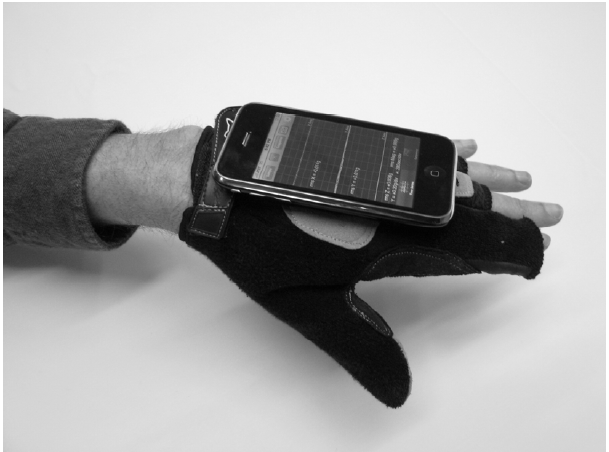
\includegraphics[scale=0.3]{./img/moyne-iphone.png}
  % matrixargseg.png: 296x162 pixel, 100dpi, 7.52x4.11 cm, bb=0 0 213 117
  %\caption{Estágio desenvolvimento de jogos ~\cite{fullerton2008game}}
\caption[Aplicação para \textit{smartphone} com a finalidade de identificar sinais de tremor]{Aplicação para iPhone com a finalidade de identificar sinais de tremor ~\cite{lemoyne2010}}
 %  \caption{Estágio desenvolvimento de jogos}
 \label{fig:iphone-tremor}
\end{figure}


Como apresentado nos trabalhos relacionados, as soluções existentes para~\ac{sms} dos sinais motores utilizam sensores vestíveis (\textit{wearables}), que comumente são incorporados à roupa ou ao corpo do usuário~\cite{classifiersparkinson2014}. De acordo com a perspectiva do usuário, estes sensores são considerados invasivos e estereotipados~\cite{aarhus_negotiating_2010}. Por outro lado, o gerenciamento medicamentoso do~\ac{dp} necessita de um cuidado acurado e diário~\cite{parkself2015,quantitativeparkinson2011}. Por este motivo, é que esta tese pretende prover um mecanismo para quantificar os sinais motores do~\ac{dp} através da indução da execução dos movimentos.


\section{Objetivos}\label{section:objetivos}
Nesta tese, tem-se como objetivo a conceber uma solução computacional que induza o usuário a executar movimentos para avaliação motora. Pretende-se usar jogos eletrônicos como forma de: \textbf{induzir}, \textbf{motivar} e abstrair o monitoramento de dados de saúde de uma maneira \textbf{não invasiva} e longe do \textbf{contexto de tratamento de saúde}.

Nesta tese, foi proposto uma arquitetura de software para o desenvolvimento de jogos eletrônicos integrados a um SMS, onde, demonstrou-se a viabilidade desta arquitetura com a implementação de um jogo capaz de monitorar um sintoma do~\ac{dp}, como estudo de caso.

%Objetivou-se criar um~\ac{sms} integrado à um jogo eletrônico capaz de: induzir a execução de uma avaliação motora que torne possível o processamento dos sinais biomecânicos e consequentemente identificar a presença de sintomas do~\ac{dp}. 

A avaliação da tese foi realizada em duas etapas: na primeira, avaliou-se a capacidade de monitoramento dos indivíduos com \ac{dp} em um estudo analítico de caso-controle; na segunda, avaliou-se a possibilidade de inserir este monitoramento na rotina diária dos pacientes. O estudo analítico de caso-controle, onde foi realizado uma avaliação com 30 sujeitos de pesquisa (15 do grupo controle e 15 diagnosticados com~\ac{dp}). Como resultado, foi identificado e quantificado o sintoma da bradicinesia. Para distinguir os grupos (caso-controle e diagnosticados com~\ac{dp}), utilizamos uma~\ac{svm} para classificação dos dados~\cite{datamining2005}, com a qual obteve-se uma acurácia de 86,66\%. Avaliou-se a adequação da abordagem de monitoramento dos sinais motores na rotina diária usando jogos eletrônicos, aplicando a técnica~\ac{gqm}~\cite{van1999goal}. Nesta avaliação, 90,00\% dos avaliados consideraram a abordagem não-invasiva e incorporável a rotina diária. 

\section{Metodologia}
Esta pesquisa foi submetida à avaliação pelo Comitê de Ética da UFCG (\textbf{CAAE: 14408213.9.1001.5182})~\footnote{Plataforma Brasil, url: http://aplicacao.saude.gov.br/plataformabrasil/} (Apêndice~\ref{sec:comite}), somente depois da aprovação deste é que os dados foram coletados. A metodologia de pesquisa possui aspectos qualitativos e quantitativos. Referente ao aspecto qualitativo, buscou-se identificar a importância desta tese junto à comunidade de especialistas da área de saúde (Seção~\ref{sec:entrevista_semi_estruturada}). Nos aspectos quantitativos, essa pesquisa fez uma análise do sensores de movimento e avaliou a acurácia da aquisição de sinais motores e possibilidade de identificar os sinais do~\ac{dp} baseado na Cinemática Angular do Movimento Humano. Por meio dos dados coletados, pudemos classificar a normalidade e dificuldade na execução de movimentos de abdução e adução dos braços~\cite{mcginnis2013biomechanics}, como será apresentado na Seção~\ref{sec:resultado_svm}. Para avaliar a aceitabilidade da proposta sob a perspectiva do usuário, utilizou-se uma análise~\ac{gqm} a qual é uma abordagem hierárquica que inicia com objetivo principal e o divide em questões mensuráveis~\cite{saraiva2006}, como será apresentado na Seção~\ref{gqm_usuarios}.

Em resumo, três questões foram utilizadas como base para a definição da metodologia do trabalho em três diferentes etapas sequenciais:
	\begin{description}
	\item[QUESTÃO 1] Quais os benefícios de acompanhar os sinais motores do paciente diariamente, do ponto de vista do profissional da saúde?
	\item[QUESTÃO 2] Como melhor adquirir e quantificar sinais motores utilizando sensores de movimento para monitorar os sinais de \ac{dp}?
	\item[QUESTÃO 3] Na perspectiva dos usuários, a abordagem de quantificar os sinais motores é considerada não-invasiva e aplicável à rotina diária?
	\end{description}

As seguintes atividades foram realizadas para a execução do trabalho:

\begin{enumerate}

\item{Realizar revisão bibliográfica e coleta de requisitos junto a profissionais de saúde.}

\item{Definir o conceito da abordagem, denominada \ac{jogue-me}, baseada em captura de sinais motores através de sensores de movimento, utilizando jogos eletrônicos e processamento dos sinais para transformá-los em informações de saúde.}


\item{Analisar a perspectiva dos profissionais de saúde em relação ao acompanhamento dos sinais motores dos pacientes com~\ac{dp} (os profissionais foram indagados sobre a melhora na tomada de decisão quanto ao acompanhamento dos sinais) e verificar se os parâmetros motores, como velocidade angular e amplitude do movimento dos braços, são importantes para realizar o acompanhamento dos sinais do~\ac{dp}. Procurou-se encontrar, junto ao profissional de saúde, a importância do monitoramento dos sinais motores e os benefícios trazidos por este, através de uma abordagem de pesquisa qualitativa. Com esta pesquisa, foi possível validar a \textbf{QUESTÃO 1}, que consiste em verificar a importância do acompanhamento de sinais motores integrados à rotina diária do paciente.}

\item{Validar o uso de sensores para classificação dos dados através do processamento dos sinais motores adquiridos por sensores de movimento utilizados em jogos eletrônicos. A classificação consistiu em aplicar os sinais numa~\ac{svm} para distinguir indivíduos do grupo controle ante indivíduos diagnosticados com~\ac{dp}.
O resultado dessa pesquisa demonstrou a viabilidade da abordagem e, consequentemente, validou a \textbf{QUESTÃO 2} do trabalho.}

\item{Definir a arquitetura de software que viabilizou tecnicamente a abordagem~\ac{jogue-me}. Nesta pesquisa, definimos um arcabouço de software para encapsular o desenvolvimento de jogos com essa abordagem.}

\item{Validar a solução~\ac{jogue-me} do ponto de vista computacional. A solução foi validada através da implementação da arquitetura e do desenvolvimento de jogos. Com esta etapa, demonstrou-se ser possível realizar monitoramento de dados motores de forma não invasiva, ou seja, sem os jogadores perceberem que estão fornecendo dados de saúde.}

\item{Verificar junto ao público alvo (portadores de~\ac{dp}) os requisitos de usabilidade, adequação à rotina diária, segurança física e se a proposta é considerada invasiva na perspectiva do paciente. Com esta avaliação, avaliou-se a \textbf{QUESTÃO 3} da pesquisa.}

\end{enumerate}

\subsection{Termo de Consentimento Livre e Esclarecido (TCLE)}
Antes da realização da coleta dos dados, expomos aos sujeitos da pesquisa as informações necessárias para a realização do estudo. Desta maneira, o indivíduo consentiu com sua participação através da assinatura do Termo de Consentimento Livre e Esclarecido~\footnote{Resolução Nº 196/96, do Conselho Nacional de Saúde, do Ministério da Saúde (CNS/MS).} (Apêndice~\ref{sec:comite}). 

\subsection{Relação Risco Benefício da Pesquisa}
Os riscos inerentes podem decorrer da exposição de dados dos participantes da pesquisa, o que pode acarretar danos morais e/ou psicológicos. Por esse motivo, foram tomados todos os cuidados para que a identidade do indivíduo não fosse revelada, garantindo assim, privacidade e confidência das informações. Todos os dados coletados, estão disponibilizados para pesquisa futura, permitindo o uso para pesquisa a todas instituições envolvidas (UFCG, UFAL e IFAL). No entanto, preservamos a identidade dos participantes da pesquisa e omitimos todos os dados que permitissem sua identificação, conforme descrito no Termo de Consentimento Livre e Esclarecido.

Durante a realização da pesquisa com os participantes da pesquisa, houve uma preocupação referente a possíveis constrangimentos por parte do sujeito da pesquisa. Caso, não conseguisse realizar a pesquisa ou responder alguma pergunta devido ao comprometimento da doença. O pesquisador prestou total assistência, orientando-os adequadamente. Mas, salienta-se que os riscos apresentados justificam-se pelo benefício de monitorar os sinais do~\ac{dp} para um melhor tratamento da doença.


\subsection{Confidencialidade}
Os dados do estudo em questão são considerados propriedade conjunta das partes envolvidas (UFCG, UFAL e IFAL). Porém, sua utilização por terceiros necessita de prévia autorização de todos. No entanto, na submissão do Projeto ao Comitê de Ética da UFCG (\textbf{CAAE: 14408213.9.1001.5182}), expressou-se o comprometimento em tornar público os resultados da pesquisa, sejam estes favoráveis ou não.


\section{Contribuições}
Nas últimas décadas, o monitoramento e quantificação dos sinais motores têm sido objeto de pesquisa recorrente na computação, eletrônica, bioinformática e saúde~\cite{reviewassesenspark2015}. As pesquisas nessa áreas, são fundamentais para a compreensão do progresso de doenças crônicas como o~\ac{dp} e também para auxiliar os médicos no acompanhamento de seus pacientes.

Nesta tese, foi desenvolvida uma arquitetura de software (Capítulo~\ref{arquitetura_captura}) que permite: quantificar, avaliar e identificar o sintoma de bradicinesia do~\ac{dp} induzindo o usuário a executar movimentos de avaliação motora, de uma forma lúdica e integrada a um jogo eletrônico, e longe do contexto de tratamento da saúde.

Do ponto de vista clínico, tornou-se possível identificar como está a saúde do paciente e em que momento o tratamento medicamentoso é eficaz. Atualmente, um detalhamento das flutuações motoras do~\ac{dp} é realizado por auto-relatórios em avaliações diárias dos pacientes que informam em que período do dia a medicação está surtindo efeito~\cite{reviewassesenspark2015}. No entanto, para uma avaliação dos sintomas motores mais acurado, é necessário poder induzir a execução de movimentos para avaliação motora de modo a mensurar quantitativamente os sintomas do~\ac{dp}~\cite{wiiassesspark2016}.

Por estes argumentos apresentados, foi desenvolvido nesta tese um mecanismo quantitativo de avaliação da eficácia do tratamento que utiliza um jogo eletrônico que induz o usuário a executar movimentos de avaliação motora de uma maneira não-invasiva. Esta abordagem de monitoramento, resulta em benefícios aos médicos para um tratamento mais efetivo e acurado da dosagem medicamentosa. Os resultados obtidos, com arquitetura de software desenvolvida, permitiu identificar e estimar a gravidade do sintoma da bradicinesia e das complicações motoras mensuradas num estudo de caso-controle, e isto é um resultado bastante relevante para esta tese.

Como possível cenário de uso da pesquisa, supondo que um paciente de uma doença crônica como o~\ac{dp} faz uso de medicamento antiparkinsoniano e possui um jogo de monitoramento de sinais do~\ac{dp} em sua residência, caso ele utilize o jogo em diferentes momentos do dia, os sinais podem ser quantificados sem a presença de um profissional de saúde, que poderia visualizar a melhora ou piora do estado de saúde do seu paciente ao longo dos dias. A partir da presente abordagem, o médico, ao possuir a informação, poderia gerenciar melhor a dosagem medicamentosa e, consequentemente, prolongar a qualidade de vida do paciente~\cite{abn2010}.

%
%Atualmente, os jogos são aplicados para melhora da saúde em diferentes contextos. No entanto, nenhum dos trabalhos relacionados pretendem identificar sinais para monitorar o estado de saúde. Logo, este trabalho visa desenvolver um ambiente de jogo que motive a execução de movimentos específicos, com o propósito de quantificar os sinais motores dos usuários.
%
%No entanto, alinhar a jogabilidade e a capacidade de monitoramento dos sinais de saúde não é trivial, pois deve ser levado em consideração o uso dos sensores e deve-se definir quais movimentos ou ações permitem a identificação dos sinais motores. Por este motivo, a proposta de um~\ac{sms} dos sinais motores usando jogos necessita de um acompanhamento de um profissional de saúde para supervisionar e auxiliar nas definições dos movimentos e ações dos usuários. 

%Posteriormente, na posse dessas ações, deverá ser testada a execução dessas atividades e sua aquisição para uma possível classificação dos dados conforme proposto nesta tese.
%os trabalhos já existentes~\cite{Ballegaard:2008:HEL:1357054.1357336,patel_monitoring_2009,visionbased2009,bachlin_parkinsons_2009,albanese2012}.
%De posse dos movimentos e da captura dos dados será feito um levantamento de um \textit{game design} que permita executar os movimentos em  um ambiente lúdico e divertido como um jogo para entretenimento ~\cite{sweetser2005-gameflow}.



\section{Organização do Documento}
O restante deste documento está organizado da seguinte forma:
\begin{itemize}
	\item No Capítulo~\ref{chapter:fundamentacao} está descrita a fundamentação teórica relacionada ao trabalho.
	\item No Capítulo~\ref{chapter:abordagem_gahme} está definida a abordagem \ac{jogue-me} para indução e monitoramento dos sinais motores de maneira não invasiva usando jogos eletrônicos.
	\item No Capítulo~\ref{chapter:arquitetura_captura} é apresentada a arquitetura de software da abordagem.
	\item No Capítulo~\ref{chap:avaliacao} são apresentados os experimentos realizados para avaliar a tese.
	\item No Capítulo~\ref{chapter:conclusoes_futuros} são apresentadas as conclusões do trabalho e propostos trabalhos futuros.
\end{itemize}

\chapter{Fundamentação Teórica}\label{chapter:fundamentacao}
Neste capítulo pretende-se oferecer ao leitor uma visão geral das principais áreas nas quais esse trabalho está fundamentado. Mais especificamente, uma explanação sobre o~\ac{dp} seus sinais motores e os estágios da doença; o uso da cinemetria como ferramenta para medição dos parâmetros cinemáticos do movimento humano e os classificadores de dados para a identificação dos padrões presentes num conjunto de dados.


%A classificação mais ampla dos tipos de jogos separa-os em jogos para entretenimento, jogos sérios (serious games) e simuladores. Em (Narayanasamy, 2006) é dado o foco da diferença entre estes três tipos de jogos na forma como são desenvolvidos, ou seja, a diferença esta no foco de seu desenvolvimento, onde jogos de entretenimento seriam jogos desenvolvidos para a diversão do usuário, jogos sérios para aprendizagem de algo especifico e simuladores para o treinamento. Porém em (Johnston e Whitehead, 2009) é apresentada uma proposta um pouco diferente e mais interessante entre estas classificações. É proposto que estes jogos não se diferenciam em sua produção, mas sim pelos jogadores que o jogam. Uma forma de vermos  isto é pensarmos em um simulador de vôo. Se colocarmos uma criança nele, esta irá se divertir e considerar aquilo como um jogo de entretenimento, enquanto um piloto profissional o consideraria um simulador.
%RETIRADO DE - ATHUS



%Para esse trabalho, é considerada a definição estabelecida por Saywer (2004) e Prensky (2001) que definem os serious games como sendo aqueles que não têm como objetivo maior a diversão ou o entretenimento, e sim, o fim educacional ou a aprendizagem sobre determinado fato, informação ou habilidade. A diversão, neste caso, continua existindo como um fator essencial para engajar o jogador no ambiente de aprendizado.
%2.1.1 Classificação dos Serious Games Michael e Chen (2006) afirmam que os serious games se diferenciam dos jogos de entretenimento pelo seu propósito final, dessa forma, eles não representam um gênero específico. Tais jogos podem assumir qualquer gênero já definido da categoria de entretenimento, desde jogos de ação, aventura, corrida, estratégia, habilidade, simulação, treinamento, educacional, entre outros
%Retirado de Sistemas Hápticos em Serious Games

%Os melhores jogos, estimulam o estado de fluxo do jogador, colocando num estado de concentração tão intenso que o mesmo perde a percepção de tempo e espaço ~\cite{kanode2009} %\apudonline{kanode2009}{calele}.
%Jogos de sucesso são mais do que \textit{software}. Um jogo pode entreter um usuário e capturar toda sua atenção, esse é o objetivo que as empresas de jogos tentam atingir ~\cite{kanode2009}.
%This paper discusses the software process of designing and developing entertainment games who enable seamless monitoring and does not attempt to address the issues involved in creative gameplay design.

%\section{Processo de Desenvolvimento de Software}
%Os processos de \textit{software} são complexos em como toda atividade que exige esforço intelectual e criativo, depende de pessoas para tomada de decisões e fazer julgamentos. Não existe um processo ideal, atualmente a maioria das organizações desenvolvem seus próprios processos de \textit{software} baseados em suas necessidades ~\cite{sommerville2011}. Para o desenvolvimento dos jogos eletrônicos é bastante comum fazer uso do modelo em cascata de desenvolvimento ~\cite{flynt2005software}  ~\cite{bethke2003game}. Porém, pesquisas indicam desafios ao aplicar processos de desenvolvimento de software em jogos eletrônicos ~\cite{kanode2009}, uma vez que o componente ``diversão'' do jogo, não pode ser sistematizado e a conseguir uma mecânica de jogo que seja divertida é necessário a execução de vários testes de protótipo até sua evolução por intermédio das iterações dentro do processo de desenvolvimento do jogo.
%
%Um processo de \textit{software} é um conjunto de atividades relacionadas às praticas necessárias para o desenvolvimento e tem como objetivo final a produção de um produto de \textit{software} ~\cite{sommerville2011}. 
%Existem muitos processos de \textit{software} diferentes, mas todos devem incluir quatro atividades fundamentais para a engenharia de \textit{software} ~\cite{sommerville2011}:
  %\begin{itemize}
   %\item \textit{Especificação de \textit{software}}: A funcionalidade do \textit{software} e as restrições a seu funcionamento devem ser definidas.
   %\item \textit{Projeto e implementação de \textit{software}}: O \textit{software} deve ser produzido para atender às especificações.
   %\item \textit{Validação de Software}: O \textit{software} deve ser validado para garantir que atenda às demandas do cliente.
   %\item \textit{Evolução de Software}: O \textit{software} deve evoluir para atender às necessidades de mudança dos clientes.
  %\end{itemize}
  

%Em um estudo, Petrillo ~\cite{petrillo2008}) identificou através de dados do \textit{Standish Group} que apenas 16$\%$ dos projetos são concluídos dentro do orçamento e tempo estabelecidos. 

%Kanode ~\cite{kanode2009}, identificou que as características de diversão são atingidas durante o desenvolvimento e teste dos protótipos. Para o autor, a prototipação deve ser realizada na fase de pré-produção do jogo para definir o que o jogo realmente é. A fase de requisitos poderia tomar lugar no final da pré-produção, uma vez que os \textit{game designers} encontraram o tipo de jogo a ser desenvolvido.

% O processo de desenvolvimento mais usado na produção de jogos é baseado no modelo em cascata ~\apudonline{. Esse processo é composto de fases que são executadas em sequencia, na qual cada fase gera artefatos de software independente dos demais. 





% \section{Processo de Desenvolvimento de Jogos}
% Os processos de desenvolvimento de \textit{software}, são categorizados como: dirigidos a planos e processos ágeis. Processos dirigidos a planos são aqueles em que todas as atividades são planejadas com antecedência, e o progresso é avaliado por comparação com o planejamento inicial. Em processos ágeis, o planejamento é gradativo, e é mais fácil alterar o processo de maneira a refletir as necessidades de mudança do cliente~\cite{sommerville2011}. A indústria de jogos eletrônicos adota processos tradicionais de desenvolvimento como os dirigidos a planos~\cite{flynt2005software,bethke2003game}. Bethke~\cite{bethke2003game} defende a adoção do \textit{The Unified Process}, por ter sido aplicado na indústria e por estar vinculado ao desenvolvimento orientado a objetos desde sua concepção. Porém o processo de desenvolvimento defendido por Bethke é bastante semelhante ao modelo de desenvolvimento em cascata~\cite{sommerville2011}.
% 
% Neste trabalho serão propostas práticas de engenharia de software e de desenvolvimento de jogos que permitam um monitoramento frequente de dados motores de saúde. Essas práticas poderão ser aplicadas em processos de desenvolvimento dirigidos a planos e ágeis, caberá ao desenvolvedor do jogo adequar essas práticas ao próprio processo.	
% %Porém, os jogos sérios com o propósito de reabilitação e monitoramento são baseados em Realidade Virtual exigem a definição dos equipamentos especiais a serem utilizados, avaliando seus benefícios no contexto do jogo. Deste modo, estereoscopia, sensações táteis, vibrações, elementos sobrepostos, monitoramento de movimentos e outras abordagens podem ser utilizados para garantir melhores resultados relacionados ao uso do jogo ~\cite{machado2011}. 
% 
% As empresas de desenvolvimento de jogos desenvolvem seus próprios processos e os aperfeiçoam conforme suas necessidades. Porém, devido a competitividade, não expõem ao público o conhecimento adquirido com a melhoria dos seus processos~\cite{origame-2012}. Por outro lado, algumas produtoras de jogos, disponibilizam  em sites especializados de jogos como o Gamasutra~\footnote{http:$//$www.gamasutra.com} \textit{postmortems} que são relatos do que ocorreu durante o desenvolvimento do projeto, como: práticas utilizadas, pontos positivos, pontos negativos, sucessos e fracassos.
% 
% Para o desenvolvimento de pesquisa na área de jogos~\cite{petrillo2008,kanode2009} os trabalhos recorrem ao uso dos \textit{postmortems} como base de conhecimento para a avaliação das técnicas usadas na indústria de jogos. Petrillo~\cite{petrillo2008}, selecionou as práticas mais utilizadas das metodologias ágeis e comparou com o que foi utilizado no desenvolvimento dos jogos, após a comparação ele analisou quais das práticas utilizadas foram positivas e negativas durante o desenvolvimento. Ao término da fase de análise ele propôs um processo de desenvolvimento ágil de jogos.
% 
% 
% %\subsection{Estágios do Processo de Desenvolvimento de Jogos}
% A indústria de jogos busca melhorar as práticas de engenharia de software para tornar o desenvolvimento de jogos mais eficiente~\cite{kanode2009}. Um dos maiores responsáveis por essas práticas é a divisão das fases de desenvolvimento. Pois cada fase são definidos marcos de desenvolvimento que precisam ser respeitados ~\cite{fullerton2008game,keith2010agile}.
% A maioria dos processos de desenvolvimento de jogos (dirigidos a planos ou ágeis) dividem o desenvolvimento do jogo em quatro fases distintas (Concepção, Pré-Produção, Produção e Pós-Produção)~\cite{kanode2009,keith2010agile,fullerton2008game,moore2011basics}. Como ilustrado nas Figuras (\ref{fig:processoful},~\ref{fig:processoful}) tanto um processo ágil dirigido a planos~\cite{fullerton2008game} quanto um processo ágil~\cite{keith2010agile}, dividem o desenvolvimento de jogos nas mesmas fases.
% 
%  %For many games developed using agile, there is still a need to separate some of the development activities ~\cite{keith2010agile}. 
% \begin{figure}[!htbp]
%  \centering
%  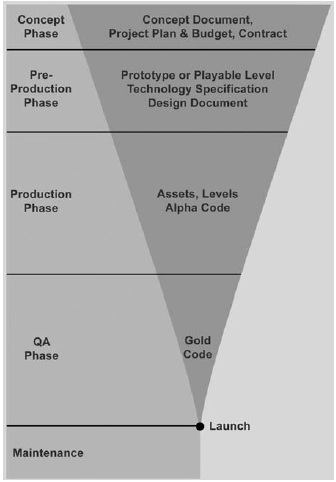
\includegraphics[scale=0.5]{./img/stages-game-development.jpg}
%  % matrixargseg.png: 296x162 pixel, 100dpi, 7.52x4.11 cm, bb=0 0 213 117~\cite{fullerton2008game}
%  %\caption{Estágio desenvolvimento de jogos ~\cite{fullerton2008game}}
% \caption[Fases de um processo de desenvolvimento de jogos dirigido a planos \copyright]{Fases de um processo de desenvolvimento de jogos dirigido a planos \copyright ~\cite{fullerton2008game}}
% %  \caption{Estágio desenvolvimento de jogos}
%  \label{fig:processoful}
% \end{figure}
% 
% Para Fullerton~\cite{fullerton2008game} no início do projeto as possibilidades criativas são grandes e por esse motivo durante essa fase ocorrem suscetíveis mudanças, porém ao longo do projeto devido a convergência de ideias e o progresso do desenvolvimento do jogo existe uma redução natural dessas modificações resultando no produto final~\cite{fullerton2008game} (Figura ~\ref{fig:processoful}).
% 
%  %For many games developed using agile, there is still a need to separate some of the development activities ~\cite{keith2010agile}. 
% \begin{figure}[!htbp]
%  \centering
%  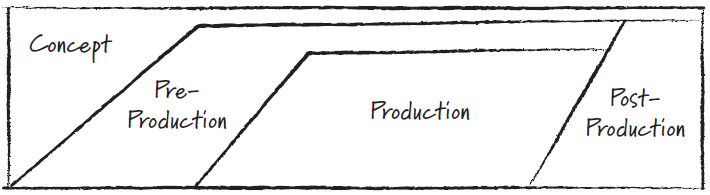
\includegraphics[scale=0.5]{./img/stages-game-development-agil.png}
%  % matrixargseg.png: 296x162 pixel, 100dpi, 7.52x4.11 cm, bb=0 0 213 117
%  %\caption{Estágio desenvolvimento de jogos ~\cite{fullerton2008game}}
% \caption[Fases de um processo de desenvolvimento ágil\copyright] {Fases de um processo de desenvolvimento ágil\copyright ~\cite{keith2010agile}}
% %  \caption{Estágio desenvolvimento de jogos}
%  \label{fig:processokeit}
% \end{figure}
% 
% 
% %inserir figura stages-game-development.png
% 
% %\subsubsection{Conceito}
% %Os requisitos para a concepção dos jogos sérios, o estímulo das funções cognitivas, a motivação e a aquisição de conhecimento são elementos fundamentais que precisam estar presentes ~\cite{machado_serious_2011}.
% 
% %Segundo Machado ~\cite{machado_serious_2011} os jogos sérios necessitam de uma colaboração estreita do especialistas da área de domínio em que o jogo está inserido. Essa colaboração irá permitir que as demais equipes responsáveis pelo desenvolvimento do jogo possam delinear o escopo do jogo e ainda assim inserir o conteúdo específico pertencente ao seu propósito ~\cite{ahn2008}.
% No desenvolvimento de um jogo tradicional, o principal objetivo da fase de conceito é conseguir o consenso entre todos os envolvidos com o primeiro marco de desenvolvimento. Infelizmente, o desenvolvimento de um jogo é uma atividade que possui muitos riscos devido sua complexidade, equipes de desenvolvimento mais experientes são mais indicadas para esses projetos~\cite{fullerton2008game}. No entanto, o desenvolvimento de um jogo com o objetivo de monitoramento de saíde possui um propósito específico logo na fase de conceito é necessário o apoio de profissionais especializados na área em que se pretende atuar. Incorporar esse profissional na equipe de desenvolvimento é necessário por permitir identificar quais serão os instrumentos e movimentos utilizados para a captura dos dados e como a coletado deve ser realizada para permitir uma melhor classificação dos dados.
% 
% Para o sucesso da abordagem deve-se pensar no público alvo e na equipe de desenvolvimento para mitigar os riscos do desenvolvimento de um jogo~\cite{fullerton2008game}. É durante a fase de conceito, em que serão testadas as tecnologias a serem utilizadas durante o desenvolvimento.
% 
% Abordagens tradicionais da engenharia de software sugerem que na fase inicial, sejam desenvolvidos protótipos de software com o objetivo de testar a tecnologia e verificar a viabilidade do projeto.
% 
% %pelo que estou lendo a fase de conceito, é para a escolha da equipe, demonstrar as capacidades técnicas e escolha da plataforma em que será desenvolvida e a habilidade do grupo naquela plataforma
% 
% %para o desenvolvimento do jogo seria interessante na fase de concepção, avaliarmos que enfermidades iríamos monitorar e avaliar as possíveis técnicas de monitoramento e testar as tecnologias que permitisse esse monitoramento.
% 
% 
% %\subsubsection{Pré-Produção}
% Na fase de pré-produção, um time pequeno faz um estudo de viabilidade da ideia. Esse time irá criar normalmente um ambiente jogável, focando nas possibilidades e riscos da tecnologia~\cite{fullerton2008game}.  A entrega de uma versão inicial que demonstre: a relevância da ideia, capacidade técnica da equipe de desenvolvimento  e os elementos de jogabilidade e diversão do jogo  são fatores cruciais para o prosseguimento nas demais etapas do processo de desenvolvimento~\cite{fullerton2008game}.
% Por se tratar de um jogo para o monitoramento, os desenvolvedores devem avaliar a capacidade de aquisição e classificação dos dados de saúde. O jogo deve ser divertido mas com o objetivo principal de adquirir dados de saúde.
% Como o estágio de pré-produção não é uma fase de construção de \textit{software}, é importante refinar o \textit{game design} do jogo, para que a documentação não fique desatualizada reduzindo os riscos potenciais do produto final~\cite{fullerton2008game}.
% 
% %\subsubsection{Produção}
% A fase de produção é a mais demorada e onerosa do desenvolvimento, o  seu objetivo é desenvolver o que foi pré-estabelecido no \textit{game design}. Nesse processo, o refinamento e melhoria do \textit{game design} é inevitável, pois os desenvolvedores passam mais tempo pensando nas soluções e consequentemente as reflete no \textit{game design}~\cite{fullerton2008game}. Nesse estágio os desenvolvedores escrevem o código criando as funcionalidades do jogo, os \textit{art designers} criam as artes e animação e os engenheiros de som criam as músicas e os efeitos sonoros, os responsáveis pelo enredo criam os diálogos e todo o contexto do jogo. A produção do jogo deve trabalhar de forma comunicativa e colaborativa para quer todos percebam o progresso do desenvolvimento do jogo~\cite{fullerton2008game}.
% 
% %\subsubsection{Pós-Produção}
% Na fase final do processo de desenvolvimento de jogos tradicionais a pós-produção é responsável por fazer o refinamento e últimos testes. Essa fase deve garantir que o jogo seja entregue com qualidade e sem erros de execução e que venha a impactar na jogabilidade. Nesse momento o jogo será testado nas diferentes plataformas para aprovar e e por fim disponibilizá-lo~\cite{keith2010agile}.

\section{Doença de Parkinson}\label{section:doenca_parkinson}
O termo Parkinsonismo é genérico e designa uma série de doenças com causas diferentes e que têm em comum a presença de sinais frequentemente encontrados no~\ac{dp}. Esta doença é uma das muitas formas de parkinsonismo, correspondendo a cerca de 75$\%$ dos casos. Os sinais associados com o~\ac{dp}~\cite{protpar010} são causados pela degeneração dos neurônios dopaminérgicos presentes na substância negra. O~\ac{dp} é mais comum em idosos, porém existem casos precoces de início da doença em indivíduos antes dos 40 anos ou até mesmo abaixo dos 21~\cite{menezes2003}. A incidência da doença é estimada de 100 a 200 casos por 100.000 habitantes e com o avanço da idade populacional o contingente de pessoas diagnosticadas com ~\ac{dp} tende a aumentar. Por ser uma doença progressiva de evolução incapacitante após os 10 a 15 anos de tratamento proporciona um enorme impacto social e financeiro. Por esse motivo, estima-se que o custo anual mundial com medicamentos antiparkinsonianos esteja em torno de 11 bilhões de 
dólares, sendo o tratamento cerca de 3 a 4 vezes mais caro para pacientes na fase avançada da doença~\cite{protpar010}. Outro fator crucial para a escolha da doença como objeto de estudo é a variação dos sinais parkinsonianos ao longo do dia em virtude da resposta ao tratamento medicamentoso. Portanto, a abordagem de monitorar os sinais em diferentes momentos do dia, permite um melhor gerenciamento da doença e como consequência uma melhora na qualidade de vida dessa população.


Atualmente, o levodopa é o tratamento medicamentoso mais utilizado para o tratamento de redução dos sinais do~\ac{dp}. Porém, sua efetividade é reduzida ao longo do tempo, requerendo um aumento progressivo das dosagens ou uso de outros tratamentos associados. Isto acarreta num gerenciamento complexo entre drogas e seus respectivos efeitos colaterais. Portanto, buscando prolongar a qualidade de vida dos pacientes no uso deste tratamento é recomendável um gerenciamento medicamentoso com uma dosagem mínima para que consiga reduzir os sinais e prolongar a qualidade de vida do paciente. O gerenciamento medicamentoso é de responsabilidade do neurologista, que faz o devido ajuste de acordo com as visitas clínicas do paciente, quando estes ou seus cuidadores fazem relatos sobre a rotina diária do paciente. Contudo, essa avaliação clínica é realizada de forma esporádica durante as consultas clínicas e de maneira subjetiva pois carece de uma avaliação tanto do paciente quanto do neurologista. 

Com o surgimento do tratamento para o \ac{dp} é possível manter uma mobilidade funcional durante anos além de aumentar a expectativa de vida dos pacientes tratados~\cite{rodrigues2006}. Os fármacos do grupo dos antiparkinsonianos como a levodopa permitem restaurar a atividade dopaminérgica que se encontra reduzida, desta maneira as drogas aliviam os sinais característicos da doença. Entretanto, devido aos efeitos colaterais frequentes induzidos pelos fármacos, é preciso iniciar o tratamento com esses medicamentos somente quando os sinais estiverem prejudicando o desempenho profissional ou nas atividades diárias do paciente~\cite{rodrigues2006}. A natureza progressiva do~\ac{dp} e suas manifestações clínicas (motoras e não motoras), estão associadas a efeitos colaterais precoces e tardios da intervenção terapêutica, o que torna o tratamento da doença bastante complexo~\cite{protpar010}. Estima-se que a taxa de morte dos neurônios dopaminérgicos da substância negra situa-se 
ao redor de 10$\%$ ao ano~\cite{national2006parkinson}. Consequentemente, com o passar do tempo, a sintomatologia parkinsoniana tende a evoluir o que aumenta a necessidade de uma maior dosagem medicamentosa, pois a resposta aos medicamentos decresce com o progresso da doença~\cite{protpar010}.

%Na evolução da doença e pela tomada do medicamento pode existir alternância entre momentos em que a medicação surte efeito e momentos em que se torna ineficaz são os chamados estados \textit{on} e \textit{off}. Alternar entre os estados \textit{on} (''normal'') e \textit{off} (``com os sinais parkisonianos'') podem depender do horário da ingestão do medicamento que tornará previsível a mudança para o estado \textit{on}. Contudo, alguns pacientes podem ter mudanças abruptas para o estado \textit{off}, sem qualquer correlação com o tempo em que a medicação foi ingerida. Essa irregularidade indetermina o momento em que o paciente entrará no estado \textit{on} ou \textit{off} e esse efeito causa impacto direto nas avaliações objetivas do profissional~\cite{patel_monitoring_2009,kostek12}.

%%Outro efeito colateral no uso do medicamento bastante conhecido é o surgimento da discinesia (movimentos involuntários de contorção) em 80$\%$ dos pacientes que recebem a levodopa como tratamento prolongado. Esse sintoma pode ser aliviado com a diminuição da dose, por outro lado, os sinais da doença tendem a retornar. Com o surgimento de discinesia intensa é necessário otimizar o gerenciamento do tratamento medicamentoso, levando a adicionar novos medicamentos para reduzir os sinais incapacitantes a longo prazo ~\cite{rodrigues2006}. 
 
\subsection{Diagnóstico}
Os mais característicos do ~\ac{dp} e que são frequentemente usados para diagnosticar a doença são~\cite{rowlandtratado}: tremor em repouso (que diminui durante movimentos voluntários); bradicinesia ou hipocinesia (lentidão e escassez de movimentos, além de dificuldade na marcha), rigidez muscular (aumento da resistência ao movimento passivo dos membros), perda de reflexos posturais que leva a alteração da marcha e aumenta a ocorrência de queda~\cite{rodrigues2006,tolosa06}. 

A evolução da doença, a gravidade e a progressão dos sinais variam de um paciente para outro. No momento não existe teste diagnóstico estabelecido para a doença e os estudos comprovam dificuldade na diferenciação clínica entre o~\ac{dp} e outras formas de parkinsonismo. A maioria dos neurologistas concordam que o diagnóstico do~\ac{dp} requer a identificação de alguma combinação de sinais motores cardinais como :tremor de repouso, bradicinesia, rigidez tipo roda denteada e alterações posturais. No entanto, uma classificação clínica padrão ainda não foi obtida ~\cite{protpar010}. Além do mais, um diagnóstico auxiliar importante é a resposta dos pacientes aos medicamentos antiparkinsonianos tal como a levodopa~\cite{protpar010}. Os protocolos clínicos sugerem que os pacientes com~\ac{dp}~\cite{protpar010} quase sempre apresentam uma resposta satisfatória a esse medicamento, e no caso de não responder satisfatoriamente à levodopa, é provável que o diagnóstico seja de outra forma de parkinsonismo. Porém, na 
literatura~\cite{rowlandtratado} uma resposta à levodopa não confirma o diagnóstico do~\ac{dp} porque existem muitos casos de parkinsonismo sintomático e muitas formas de síndrome de Parkinson em seus estágios iniciais que também respondem à levodopa. 

Atualmente, os critérios estabelecidos pelo Banco de Cérebros da Sociedade de Parkinson do Reino Unido são os mais utilizados para diagnosticar a doença~\cite{protpar010} (Apêndice \ref{apendice:diagnostico_parkinson}). 

%Como pouemos perceber ao longo desta seção, os estudos demonstram as dificuldades na diferenciação clínica entre o ~\ac{dp} e outros tipos de parkinsonismos. No entanto, através da revisão de diagnósticos patológicos e clínicos, um grupo de neurologistas especializados em distúrbios de movimento do \textit{National Hospital for Neurology and Neurosurgery} de Londres, conseguiu um valor preditivo de diagnóstico da doença em 98,6$\%$. 


\subsection{Principais Sinais do Parkinson}
Nesta seção serão descritos sintomas motores mais frequentes do~\ac{dp}~\cite{protpar010} e que foram objetos deste estudo. %\subsubsection{Prevenção de Flutuações Motoras e Discinesias}
%Um dos benefícios teóricos dos agonistas dopaminérgicos sobre a dopamina é uma meia-vida longa, resultando em menor estimulação pulsátil dos receptores de dopamina, o que poderia reduzir o risco do desenvolvimento de flutuações motoras e discinesias ~\cite{protpar010}.
%
%Os pacientes tratados com levodopa apresentam maior número de flutuações motoras e discinesias do que os tratados com pramipexol e cabergolina ~\cite{rasc2000,rinne98}. No entanto, estas diferenças entre agonistas e levodopa parecem desaparecer a longo prazo, pois estudos com mais de uma década de seguimento sugerem que os pacientes acabam tendo a mesma frequência de complicações motoras independentemente do tratamento que receberam nos primeiros anos da doença ~\cite{haus07,katzen08}. Com base nestes dados, tem sido recomendado que indivíduos mais jovens iniciem o tratamento sintomático com os agonistas da dopamina, por apresentarem maior risco das complicações motoras com levodopa ~\cite{silv98,acaneuro02,koll02}. Porém, se os sinais motores não forem bem controlados com doses adequadas de agonistas dopaminérgicos, levodopa deve ser logo adicionada a eles.

\subsubsection{Tremor}\label{sec:tremor}
O tremor é o sintoma mais frequente e mais perceptível~\cite{limongi2002} do~\ac{dp}, embora não seja o mais incapacitante. No entanto, para a maioria dos pacientes este sinal é o principal motivo que os leva a procurar ajuda médica. Apresentando-se de forma característica: rítmico, relativamente lento quando comparado com outros tipos de tremor (4 a 7 ciclos por segundo) onde sua maior frequência é quando o membro está em repouso sendo denominado de tremor de repouso. No início da enfermidade, o tremor ocorre em um lado (tremor assimétrico) e assim permanece por diferentes período de tempo. Situações de estresse emocional, ou a sensação de ser observado aumentam visivelmente a intensidade do tremor~\cite{jankovic2008}. 

Por ser um sinal relacionado ao repouso do membro os usuários cessavam o sinal assim que eram confrontados com um jogo eletrônico desenvolvido para quantificação do tremor. Desta forma, não foi possível desenvolver um jogo para celular com o objetivo de quantificar este sinal.


\subsubsection{Bradicinesia}\label{section:analise_bradicinesia}
Enquanto que o sintoma de tremor é mais visível do~\ac{dp}, a bradicinesia é o sintoma mais incapacitante da doença. A bradicinesia consiste numa lentidão do movimento voluntário e num comprometimento de todos os movimentos associados a ele. A acinesia é uma progressão da bradicinesia e implica na ausência completa do movimento voluntário sem a perda da força muscular~\cite{do2007parkinson}.

A bradicinesia pode estar presente nos sinais iniciais do~\ac{dp}, em diferentes partes do corpo: olhos com a redução do movimento de piscar, face com a redução das expressões faciais, voz pela redução da velocidade dos músculos das cordas vocais e membros~\cite{do2007parkinson}. Normalmente nos estágios iniciais da doença a bradicinesia é acompanhada de uma rigidez dos músculos, apresentando uma assimetria dos movimentos entre os membros, ocasionando dificuldade em levantar de uma cadeira, virar na cama ou andar. Os sinais bradicinéticos são avaliados por intermédio da parte motora da tabela de avaliação UPDRS~\cite{updrs87}, através de exercícios como tocar as pontas dos dedos, pronação e supinação do antebraço. 

\subsection{Escalas e os Estágios da Doença}\label{section:escalas_avaliacao}
A partir dos tratamentos para a~\ac{dp}, foram criadas escalas de avaliação do progresso da doença~\cite{updrs87,Hoehn_Yahr_2001}. Essas escalas permitem avaliar: a condição clínica geral, incapacidades, funções motoras, mentais e até mesmo a qualidade de vida dos pacientes. Esses instrumentos são importantes tanto no nível clínico quanto no científico, pois permitem monitorar a progressão da doença e a eficácia do tratamento medicamentoso~\cite{updrs87,goul05}.  Por conseguinte, foi criada em 1987 a Escala Unificada de Avaliação da  Doença de Parkinson (\textit{Unified Parkinson’s Disease Rating Scale – UPDRS})~\cite{updrs87} que é amplamente utilizada para monitorar o progresso da doença e a eficácia do tratamento. Segundo Goulart~\cite{goul05} as escalas de estágios de incapacidade representadas por: \textit{Hoehn/Yahr}~\cite{Hoehn_Yahr_2001} e a \textit{UPDRS}~\cite{updrs87}, são consideradas as de maior confiabilidade, podendo ser usadas por fisioterapeutas para melhor avaliação do estado clínico-
funcional do  paciente.% 
% Atualmente a evolução da \ac{dp} é avaliada através de escalas, que permitem avaliar a eficácia do tratamentos e sua aplicabilidade nas práticas fisioterápicas. Segundo um trabalho de Goulart ~\cite{goul05} as escalas de estágios de incapacidade representadas por Hoehn/Yahr ~\cite{Hoehn_Yahr_2001} e a UPDRS ~\cite{updrs87} são consideradas as de maior confiabilidade, podendo ser usadas por fisioterapeutas para melhor avaliação do estado clínico-funcional do  paciente.

Segundo a \textit{UPDRS} a evolução do~\ac{dp} é classificada nas seguintes fases ~\cite{updrs87}:
  \begin{itemize}
    \item \textbf{ESTÁGIO 0:} Nenhum sinal da doença;
    \item \textbf{ESTÁGIO 1:} Doença unilateral;
    \item \textbf{ESTÁGIO 1,5:} Envolvimento unilateral e axial;
    \item \textbf{ESTÁGIO 2:} Doença bilateral sem déficit de equilíbrio;
    \item \textbf{ESTÁGIO 2,5:} Doença bilateral leve, com recuperação no “teste do empurrão”;
    \item \textbf{ESTÁGIO 3:} Doença bilateral leve a moderada; alguma instabilidade postural; capacidade para viver independente;
    \item \textbf{ESTÁGIO 4:} Incapacidade grave, ainda capaz de caminhar ou permanecer de pé sem ajuda;
    \item \textbf{ESTÁGIO 5:} Confinado à cama ou cadeira de rodas a não ser que receba ajuda.
  \end{itemize}

A \textit{UPDRS} é composta por 42 itens, divididos em quatro partes (atividade mental, comportamento e humor, atividades de vida diária e exploração motora e complicações da terapia medicamentosa) e através da avaliação desses sinais, por intermédio do auto-relato e da observação clínica, é possível classificar em que estágio da doença o paciente se encontra. Contudo, justamente por ser baseada em auto-relato e observação clínica a qual é realizada eventualmente com a presença de um profissional, pesquisadores questionam a efetividade da análise do estágio da doença e propõem alternativas para avaliação dos itens motores de forma quantitativa através de sensores, os quais permitem monitorar o estágio do paciente~\cite{kostek12,synnott_wiipd_2012,patel_monitoring_2009}.

%Alguns sinais parkisonianos são consequências do longo período do uso da medicação seja ela levodopa ou dopaminérgicos~\cite{protpar010}. No início do tratamento, o levodopa irá melhorar consideravelmente a qualidade de vida do paciente e poderá permanecer nesse estado por anos. Mas com o passar dos anos a efetividade do levodopa diminuirá e o paciente irá alternar entre os estados \textit{on} e \textit{off}. Por esse motivo, a detecção das alterações dos estágios da doença dentro de curtos períodos é complicada, em particular porque os testes a partir das escalas são aplicados de forma objetiva por um profissional, que avalia  evolução do quadro periodicamente de três a seis meses. Isso se torna um obstáculo tanto para o paciente quanto a disponibilidade do profissional, deve ser mencionado também que a precisão da avaliação dependerá das capacidades motoras e do tempo em que o medicamento foi ingerido.
% (``com os sinais parkisonianos''). As mudanças dos estados \textit{on} para \textit{off} dependerá do agendamento da ingestão do medicamento que tornará previsível a mudança para o estado \textit{on}. Contudo, alguns pacientes, podem ter mudanças abruptas para o estado \textit{off}, sem qualquer correlação com o tempo em que a medicação foi ingerida, isso é chamado do fenômeno \textit{on-off} e mudanças do estado \textit{on} ou \textit{off} podem ocorrer [~\cite{patel_monitoring_2009}. Essa irregularidade de não conseguir determinar o momento em que o paciente entrará no estado \textit{on} ou \textit{off} impacta diretamente nas avaliações objetivas do profissional que irá avaliar os estágios da doença fazendo uma avaliação errada ~\cite{patel_monitoring_2009}.

A identificação dos sinais do~\ac{dp} durante a rotina diária permite um diagnóstico mais precoce da doença e consequentemente obter seus benefícios de um tratamento mais duradouro. Além disso, o monitoramento dos efeitos da medicação junto ao paciente permite um melhor gerenciamento medicamentoso e consequentemente reduz os efeitos colaterais do tratamento e prolonga sua qualidade de vida~\cite{rowlandtratado}.


\section{Cinemetria}
A \textbf{Cinemetria} consiste de um conjunto de métodos para medição dos parâmetros cinemáticos do movimento como: posição, orientação, velocidade e aceleração~\cite{biomecanica99}. Os instrumentos básicos das medidas cinemáticas podem ser adquiridos por câmeras de vídeo durante a análise das imagens e dos movimentos por meio de software específico os quais calculam as variáveis cinemáticas de interesse. Atualmente, com o uso de câmeras infravermelho, é possível reconhecer o movimento humano e calcular as grandezas cinemáticas das características do movimento com precisão e robustez~\cite{gabel2012}.

A cinemetria relaciona técnicas e métodos para o processamento de grandezas cinemáticas, entre elas destacamos as técnicas de medição direta~\cite{biomecanica99}, utilizadas para: 
\begin{enumerate}
	\item medidas de tempo;
	\item medidas de ângulos;
	\item medidas de amplitude;
	\item medidas de velocidade angular.
\end{enumerate}

% \subsection{Movimento Cinético}
% Movimento Cinético é o estudo das forças e momentos que resultam no movimento do corpo e seus segmentos, incluindo a mensuração da \ac{fvrs} e análise cinética. A Medição Cinética é realizada das forças presentes entre o pé e o solo, a qual é medida por intermédio de sensores de força que permitem adquirir a pressão do pé em relação ao solo. Estudos indicam que por meio da análise do movimento cinético é possível avaliar o desempenho do corpo durante a execução das atividades diárias~\cite{gaitusingsensorsreview2012}.
% 
% Nos últimos anos com os sensores de movimento vestíveis, foi possível evoluir os estudos sobre a análise de marcha em ambientes que não fossem somente os laboratórios e clínicas, os quais possuíam placas de força e esteiras eletrônicas que permitem realizar o estudo~\cite{gaitusingsensorsreview2012}. Pode ser salientado também, que por meio destes dispositivos o monitoramento contínuo da marcha pode ser possível mensurar e quantificar os ciclos de movimento de cada usuário na sua rotina diária e consequentemente identificar sinais relativos a marcha.


%==========================
% Sensores
%==========================
%In gait analysis using wearable sensors, motion sensors are worn or attached to various parts of the patient’s body, such as the foot and waist. These sensors, which may be accelerometers, gyrosensors, force sensors, strain gauges, inclinometers, goniometers, and so on, can measure various characteristics of the human gait [20,21]. The movement signal recorded by these sensors can be used to perform the gait analysis ~\cite{gaitusingsensorsreview2012}.

%-------------------------------
%2.2.1. Accelerometer, Gyroscope, and Magnetoresistive Sensors
%-------------------------------
%An accelerometer is a type of inertial sensor that can measure acceleration along its sensitive axis. The common operation principle of accelerometers is based on a mechanical sensing element that comprises a proof mass attached to a mechanical suspension system, with respect to a reference frame.
%The mass proof can be forced to deflect by the inertial force because of acceleration or gravity according to Newton’s second Law (force = mass × acceleration). Based on this principle, the acceleration can be measured electrically using the physical changes in the displacement of the proof mass, with respect to the reference frame.
%Three common types of accelerometers are available, namely, piezoelectric, piezoresistive, and capacitive accelerometers [35]. Piezoresistive and capacitive accelerometers can provide dual acceleration components and have higher stability. Thus, these types of accelerometers are suitable for measuring the motion status in the human gait [36]. By attaching these accelerometers to the feet or legs, the acceleration/velocity of the feet or legs in the gait can be determined to perform the gait analysis [37].
%~\cite{gaitusingsensorsreview2012}

%Force Sensors
----------------------------
%----------------------------------
% Attention here he talks about vertical ground reaction forces
%----------------------------------
%Slavelberg and Forner-Cordero reported on estimates of the three-dimensional (3D) ground reaction forces (GRFs) from the insole based on foot pressure data [28,29]. With the development of motion-sensing technology, an increasing number of wearable sensors will be developed for gait analysis in the future. Gait analysis using wearable sensors will thus be widely used in the clinical field.
%~\cite{gaitusingsensorsreview2012}

%Force sensors can be embedded into footwear to realize ambulatory measurements of GRF during the gait. This GRF is a 3D vector, with the actual direction depending on the nature of the interface between the foot and the ground. In the development of wearable force sensors, various implementations of the force transducer, including piezoelectrics [68,69], strain gauged [70,71] and capacitive transducerd [72–74], are feasible. In addition, Hessert et al. designed a type of wearable force sensor based on a photoelastic triaxial force transducer to measure GRF in gait analysis [75]. Force sensors based on the optical fiber matrix were developed to detect the shear and compressive force during human walking [76,77].
%~\cite{gaitusingsensorsreview2012}

%---------------------------
% Kinnect
%---------------------------
%We propose a low-cost, non-intrusive system that can accurately measure a wide range of gait parameters using the Kinect sensor and Software Development Kit (SDK). Kinect is an array of sensors, including a camera and a depth sensor. In addition to the raw depth image, Kinect extracts a 3D virtual skeleton of the body [17]. These capabilities, packed in an affordable and compact device, already led several researchers to propose its use for home monitoring and gait analysis [18], [19].
%We apply a supervised learning approach to automatically and accurately extract lower and upper body gait parameters, using the 3D virtual skeleton. This allows us to go beyond standard foot stride parameters. For example, we extract arm kinematics using the same sensor. We show that our method is accurate and robust to attributes such as sensor position. Moreover, our method can be extended to measure other properties such as leg kinematics.
%In this work we have presented a novel method for full body gait analysis using the Kinect sensor. Using the virtual skeleton as the input to a learned model, we demonstrated accurate and robust measurements of a rich set of gait features.In this work we have presented a novel method for ful body gait analysis using the Kinect sensor. Using the virtual skeleton as the input to a learned model, we demonstrated accurate and robust measurements of a rich set of gait features.
%~\cite{gabel2012}


%===========================
%Dificuldades
%==========================


%===========================
%4. Application of Gait Analysis Using Wearable Sensors
%===========================
%With the development of sensor technology and gait data analyzing techniques, gait analysis using wearable sensors has become a widespread and useful tool for both clinical practice and biomechanical research. Using small, low-power, and low cost wearable sensors, ambulatory gait analysis can be used conveniently in sports, rehabilitation, and clinical diagnostics, as summarized in the following. %~\cite{gaitusingsensorsreview2012}

% 4.3. Clinical Diagnosis and Healthcare Monitoring
%In the clinical diagnosis of patients with Parkinson’s or knee osteoarthritis disease, the ambulatory estimation of lower extremity movement in the gait is usually necessary [172]. Based on the estimation results of the lower extremities, the disease and its severity can be determined, and clinicians can establish a proper treatment scheme for the patients. In healthcare monitoring, gait analysis based on wearable sensors can also be applied in various occasions, such as in the detection of gait abnormalities, the assessment of recovery, fall risk estimation, and so on. In the healthcare environment, gait information is used to detect walking behavior abnormalities that may indicate the onset of adverse health problems or the progression of neurodegenerative diseases [173]. The presence of gait abnormalities in elderly persons is often a significant predictor of the risk of the development of dementia, especially non-Alzheimer’s dementia [174].
%~\cite{gaitusingsensorsreview2012}

%Passos para análise

\subsection{Movimento Angular}
O movimento angular ocorre quando todas as partes do corpo se movem pelo mesmo ângulo mas não realizam o mesmo deslocamento linear. A subdivisão da cinemática que trata com o movimento angular é chamada de cinemática angular, que permite examinar o movimento angular a partir de segmentos de um movimento, divididos em partes identificáveis que aumentam a compreensão do movimento humano~\cite{hamill1999bases}. 

Quase todos os movimentos humanos envolvem as rotações de segmentos do corpo, os segmentos giram sobre os centros articulares que formam os eixos de rotação para esses segmentos~\cite{hamill1999bases}. No movimento angular, a unidade de medida utilizada é o grau (º) e a unidade de tempo é o segundo (s). Logo as velocidades angulares calculadas são medidas em °/s.

A anatomia funcional consiste no estudo dos componentes do corpo necessários desempenhar um movimento ou função humana como por exemplo a abdução ou adução do braço (Figura \ref{fig:movabducaoaducao}).

\begin{figure}
 \centering
 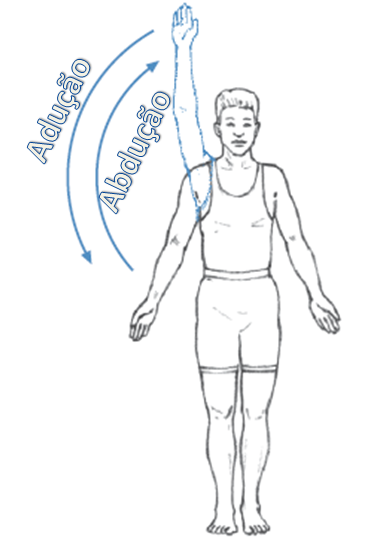
\includegraphics[scale=0.5]{./img/abducao.png}
 % matrixargseg.png: 296x162 pixel, 100dpi, 7.52x4.11 cm, bb=0 0 213 117
 %\caption{Estágio desenvolvimento de jogos ~\cite{fullerton2008game}}
\caption[Movimentos de Abdução e Adução do Braço]{\copyright Movimentos de Abdução e Adução do Braço~\cite{mcginnis2013biomechanics}}
%  \caption{Estágio desenvolvimento de jogos}
 \label{fig:movabducaoaducao}
\end{figure}

Na análise biomecânica do movimento humano, são calculados dois tipos de ângulos:
	\begin{itemize}
		\item Ângulo Relativo: este ângulo é formado entre os eixos longitudinais de segmentos corporais adjacentes~\cite{hamill1999bases}. Logo, os ângulos relativos, não descrevem a posição de segmentos ou os lados do ângulo no espaço. Se um indivíduo tem um ângulo relativo de 90º no cotovelo e esse ângulo é mantido, o braço pode ficar em qualquer posição. A interpretação dada a cada segmento irá determinar o tipo de movimento realizado. 
		\item Ângulo Absoluto: este ângulo identifica a orientação angular de um segmento corporal em relação a uma linha fixa de referência~\cite{hamill1999bases}. Logo, os ângulos absolutos devem ser medidos na mesma direção a partir de uma única referência seja ela horizontal ou vertical.
	\end{itemize}


%A interpretação correta de flexionar o braço pode ser levantar todo o braço, já que braço refere-se ao úmero, não ao rádio e à ulna. Uma revisão dos nomes dos segmentos é indispensável no preparo para o uso mais extensivo deles no estudo da biomecânica ~\cite{hamill1999bases}.

\section{Máquinas de Vetor de Suporte (SVM)}\label{sec:svm_linear}
A teoria da aprendizagem estatística, fornece um conjunto de técnicas para a análise de dados a qual permite a aquisição de conhecimento ~\cite{vapnik95}. As máquinas ~\ac{svm}, fazem uso de um conjunto de métodos de aprendizagem supervisionada para classificação de dados. Ou seja,~\ac{svm} é uma ferramenta de predição de classificação que usa a teoria da aprendizagem de máquina que busca maximizar a acurácia. Normalmente, a~\ac{svm} é aplicada para classificação binária, ou seja permite classificar os dados em duas classes, porém essa técnica pode ser aplicada para em dados e que possuam mais de duas classes.

Um classificador ~\ac{svm} foi inicialmente desenvolvido para problemas de aprendizagem linearmente separáveis. Utilizando vetores de separação através de uma técnica de hiperplano de separação ótima ~\cite{vapnik95}. O hiperplano tenta separar as diferentes classes, maximizando a margem entre os pontos extremos de cada classe~\cite{valt2010}. O melhor hiperplano de uma~\ac{svm} significa é aquele que possui a maior margem entre as duas classes como pode ser visto na Figura ~\ref{fig:hiperplano}.  

\begin{figure}
 \centering
 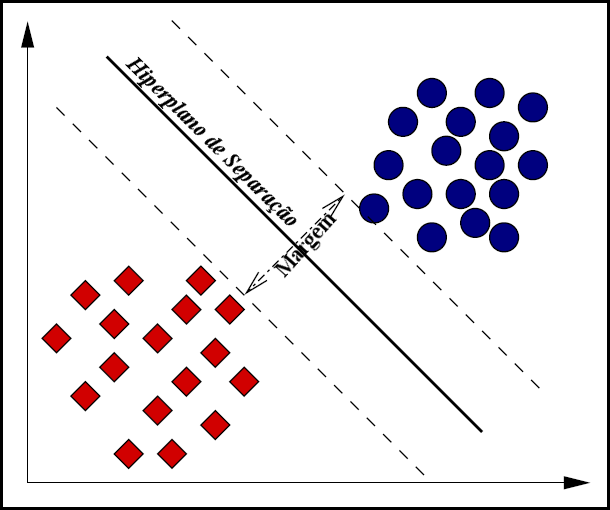
\includegraphics[scale=0.4]{./img/svmhyperplane.png}
 % matrixargseg.png: 296x162 pixel, 100dpi, 7.52x4.11 cm, bb=0 0 213 117
 %\caption{Estágio desenvolvimento de jogos ~\cite{fullerton2008game}}
\caption{Hiperplano de Separação Linear Para Duas Classes}
%  \caption{Estágio desenvolvimento de jogos}
 \label{fig:hiperplano}
\end{figure}


Para entender o funcionamento da ~\ac{svm} é necessário conhecer a notação:
\begin{math}
R^{n}
\end{math}
é um número real n-dimensional no espaço de vetores. Onde os pontos \textbf{u}, \textbf{v}, \textbf{w} e \textbf{x} serão utilizados para denotar pontos em 
\begin{math}
R^{n}
\end{math}.
Estes pontos são chamados de vetores ou padrões na literatura de Aprendizagem de Máquina.

Cada ponto possui $x_{i}$ e um rótulo $y_{i}$ que denota a qual classe $x_{i}$ pertence. Logo, se $y_{i} = + 1$ e $x_{i}$ pertencer a classe 1 e $y_{i} = - 1$ caso o $x_{i}$ pertencer a classe 2. A classificação binária como o nome sugere, significa classificar os dados em duas classes. Para tanto, primeiramente os dados do grupo de treinamento são usados para preencher os espaços com pontos. E depois um segundo grupo de teste é aplicado para verificar a hipótese de qual classe aquele ponto pertence. Formalmente, dado um conjunto de pontos $x_{i}$ qual será os valores $y_{i}$ correspondentes. Dado que o classificador possui os padrões adquiridos do grupo de treinamento além dos rótulos associados a sua classe. A~\ac{svm} irá usar o hiperplano de separação para tentar dividir os dados de treinamento em duas classes. Logo, o resultado da classificação dos dados de teste dependerá da localização da projeção desses dados.

Formalmente, classificadores que separam os dados por meio de um hiperplano utilizam um discriminante linear~\cite{valt2010} de Equação~\ref{eq:hiperplano}. Um hiperplano é considerado de Margem Máxima (ou de Separação Ótima) quando separa um conjunto de vetores sem erro e a distância entre os vetores (das classes opostas) mais próximas ao hiperplano é máxima por intermédio de uma função discriminante. Uma função é discriminante quando consegue discriminar os valores em diferentes padrões. 

O produto escalar $ w.x $ entre os vetores $ w $ e $ x $, $ w $ é o vetor normal ao hiperplano descrito e o vetor \textbf{w} é denominado de peso e a constante parâmetro \textbf{b} é chamada de \textit{bias} ou desvio.
\linebreak
\begin{equation}
f(x)=w^Tx+b=0
\label{eq:hiperplano}
\end{equation}

Se \textbf{u} e \textbf{v} são dois padrões e \textit{f()} é a função discriminante, então os valores de \textit{f(\textbf{u})} e \textit{f(\textbf{v})} irá auxiliar em determinar se os valores de \textbf{u} e \textbf{v} pertencem a classe, logo a regra para a predição da classe está no Código~\ref{codepredicaoclasse}. 

\begin{lstlisting}[frame=single, caption=Código de Predição da Classes, label=codepredicaoclasse]  % Start your code-block

classificacao = 0;
if (w^t.x + b > = 0)
	classificacao = 1
else
	classificacao = -1;
endif
\end{lstlisting}
A partir desse método de separação de dados lineares é que a~\ac{svm} foi aplicada para classificar indivíduos diagnosticados com ~\ac{dp} ante indivíduos sem o diagnóstico estabelecido. Na Seção~\ref{sec:processador_bio}, será explicado como são extraídos os pontos usando os vetores de características para obtenção da classificação exposta na Seção~\ref{sec:resultado_svm}.


%\chapter{Processo de Desenvolvimento do \textit{GAHME Component}}
A engenharia de software baseada em reúso de software é uma estratégia em que o processo de desenvolvimento é orientado para reúso de \textit{softwares} existentes ~\cite{sommerville2011}. Uma abordagem de reúso bastante adota é fazer uso de componentes de \textit{software}que são entidades desenvolvidas com o propósito de serem reutilizadas, incorporando seus comportamentos e funcionalidades no desenvolvimento de novos \textit{softwares}. Essa é uma abordagem é eficaz para esconder a complexidade de um conhecimento especializado que pode ser encapsulado por intermédio do uso dos componentes de software ~\cite{sommerville2011}.

Levando em consideração que os o desenvolvimento de componentes de software para monitoramento de dados de saúde aplicados a jogos eletrônicos (\textit{GAHME Component}), possuem uma complexidade inerente ao domínio em que são aplicados (Saúde). Domínio esse, que necessita de um especialista de domínio (Profissionais de Saúde) para a sua concepção, elaboração e desenvolvimento. Outro grande problema desse contexto é a verificação da eficácia do monitoramento junto aos seres humanos, pois de acordo com as normas regulamentadoras previstas para pesquisa envolvendo seres humanos segundo a Resolução 196/96 ~\cite{conselho2000normas}, qualquer atividade de pesquisa que envolva seres humanos é necessário a submissão a um Comitê de Ética que permita a coleta dos dados. Esse processo leva tempo e pode impactar na produção dos jogos eletrônicos com propósito de monitoramento dos dados de saúde. Logo, se for possível encapsular o conhecimento de domínio em um componente e verificar sua eficácia ~\cite{kato12} junto a seres humanos então os softwares produzidos com o uso destes componentes irão incorporar esse comportamento e não precisarão passar por todo processo de concepção, elaboração e validação da pesquisa em saúde.

Corroborando com esse contexto, Sommerville ~\cite{sommerville2011} cita benefícios do reúso de software que se encaixam perfeitamente neste trabalho:
	\begin{itemize}
		\textbf{Confiança aumentada:} Os softwares reusados, experimentados e testados em sistemas em funcionamento provavelmente são mais confiáveis do que um novo software. Os defeitos podem ser encontrados corrigidos e incorporados novamente nos sistemas melhorando-o continuamente.
		\textbf{Uso Eficaz de especialistas:} Em vez de fazer o levantamento do domínio a ser estudado, os especialistas podem desenvolver \textit{softwares} reusáveis que encapsulam o seu conhecimento;
		\textbf{Desenvolvimento acelerado:} O reúso de um software pode acelerar a produção de um sistema, pois reduz o tempo de desenvolvimento e validação.
	\end{itemize}

A \ac{cbse} surgiu na década de 1990 como uma abordagem para softwares de desenvolvimento de sistemas com base no reúso de componentes de software ~\cite{sommerville2011}. Os componentes são abstrações de nível mais alto do que objetos definidos por usas interfaces. Geralmente eles são maiores que objetos individuais e todos os detalhes de implementação são escondidos de outros componentes ~\cite{sommerville2011}.

Utilizando as técnicas \ac{cbse}, é possível definir, implementar, integrar ou compor componentes independentes, e de fraco acoplamento facilitando o reúso do software ~\cite{bezerra2007}. Essa abordagem facilitou o desenvolvimento de \textit{softwares} cada vez mais complexos, pois por intermédio do reúso e do encapsulamento proporcionado pelos componentes, é possível desenvolve-los e implanta-los com mais agilidade e robustez.  

De acordo com Sommerville ~\cite{sommerville2011}, o desenvolvimento baseado em componentes faz uso de boas práticas de Engenharia de Software, por esse motivo os componentes eles possuem:
	\begin{itemize}
		\item \textbf{Encapsulamento :} como os componentes são especificados por suas interfaces, eles possuem separação entre a definição (interface) e sua implementação. Detalhes de implementação estão encapsulados, podendo ser alterados, modificados sem afetar todo o sistema;
		\item \textbf{Comunicação :} Os componentes comunicam-se por meio de interfaces bem definidas. Se estas interfaces forem mantidas, um componente poderá ser substituído por outro, que forneça melhores resultados;
		\item \textbf{Reúso :} Os componentes devem ser passíveis de composição, todas as interações externas devem ter lugar por meio de interfaces publicamente definidas, permitindo o reúso de software reduzindo o esforço e o tempo gasto de desenvolvimento.		
		\item \textbf{Documentação :} Os componentes devem ser completamente documentados para que os desenvolvedores, possam verificar sua especificação e sua aplicabilidade.
	\end{itemize}

\section{Processo CBSE}
Os processos CBSE são processos de software que oferecem suporte a engenharia de software baseada em componentes. Nesses processos são considerados as possibilidades de reúso e as atividades envolvidas no desenvolvimento e uso de componentes de \textit{software} reusáveis.
Segundo Sommerville ~\cite{sommerville2011}, num nível mais alto existem dois tipos de processo CBSE:
	\begin{enumerate}
		\item \textbf{Desenvolvimento para reúso:} Esse processo está interessado no desenvolvimento de componentes ou serviços que serão reusados em outras aplicações. Esse processo busca generalizar os componentes existentes facilitando o reúso.
		\item \textbf{Desenvolvimento com reúso:} Esse é o processo de desenvolvimento de novas aplicações usando o componentes existentes.
	\end{enumerate}  

O processo básico de um \ac{cbse} (Figura \ref{fig:process-cbse}) com e para reúso apoiam os processos que estão preocupados com a aquisição do componente, gerenciamento de componente e certificação de componente ~\cite{sommerville2011}:

\begin{itemize}
	\item \textbf{Aquisição de componente :} é o processo de aquisição de componentes para reúso ou desenvolvimento em um componente reusável;
	\item \textbf{Certificação de componente :} é o processo de verificação e certificação de que um componente atende a sua certificação.
\end{itemize}

Os componentes podem ser disponibilizados em um repositório, que incluirá as documentações e especificações para o seu uso.

\begin{figure}
 \centering
 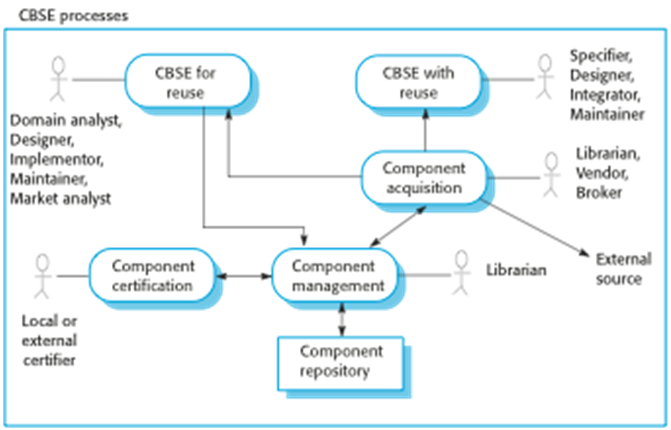
\includegraphics[scale=0.8]{./img/cbse-kot.png}
 % matrixargseg.png: 296x162 pixel, 100dpi, 7.52x4.11 cm, bb=0 0 213 117
 %\caption{Estágio desenvolvimento de jogos ~\cite{fullerton2008game}}
\caption{Processo CBSE}
%  \caption{Estágio desenvolvimento de jogos}
 \label{fig:process-cbse}
\end{figure}

Para a elaboração deste processo foi realizada uma revisão da literatura sobre desenvolvimento de jogos tradicionais (Capítulo \ref{cap:desenvolvimento_jogos}) ~\cite{keith2010agile,moore2011basics,rucker2003,kanode2009} software e das necessidades encontradas no desenvolvimento de jogos voltados para saúde como ~\cite{Suhonen_2010,herber2011,bartolome11,sinclair07,Hardy2011,kato12}. O objetivo desta seção definir um processo de desenvolvimento voltado para reúso que permite desenvolver componentes de \textit{software} a serem integrados em  jogos para entretenimento. Nossa proposta é que esses componentes permitem o monitoramento de dados de saúde de modo não invasivo e integrado a rotina da vida diária.

%Para a elaboração desse processo foram utilizados estudos empíricos através de técnicas de pesquisa qualitativa com o uso de entrevista semi-estruturada \cite{FLI04} e observação participativa em um estudo de caso \cite{Yin05}. O resultado dessas avaliações estã descritos na \secref{section:analise_entrevista_semi_estruturada}. Como resultado dessa análise foram extraídos requisitos (\secref{section:requisitos_entrevista} e \secref{section:requisitos_estudo_caso}) que definiram algumas características e problemas de ambientes distribuídos de desenvolvimento, os quais requerem maior atenção em relação ao desenvolvimento presencial, como: uso de ferramentas colaborativas, meios de comunicação e coordenação das equipes distribuídas. 
%Como procuramos propor um processo completo para ser customizado a toda e qualquer aplicação, é importante que a equipe de desenvolvimento faça uma análise inicial do processo como um todo e de acordo com suas necessidades avalie que atividades e artefatos devem ser instanciados para o projeto.

A modelagem deste processo fez uso da semântica do meta-modelo \ac{spem} na Versão 2.0 \cite{spem08} que permite modelar métodos, atividades de processos de software através da notação gráfica UML. O SPEM 2.0 é usado para definir processos de desenvolvimento de software, sistemas e seus respectivos componentes. O escopo da SPEM se restringe aos elementos necessários para definir qualquer processo de desenvolvimento de software, sem adicionar funcionalidades específicas para domínios particulares (como por exemplo, desenvolvimento de um jogo).

Como pode ser visto na Figura \ref{fig:spem20}, o meta-modelo está estruturado em sete pacotes de meta-modelos. A estrutura divide o modelo em unidades lógicas com responsabilidades bem definidas e cada unidade compartilha informações gerando dependências entre elas sendo capaz de suportar diferentes variedades de clico de vida, como: em cascata, iterativo e incremental, evolucionário e assim por diante.

\begin{figure}
 \centering
 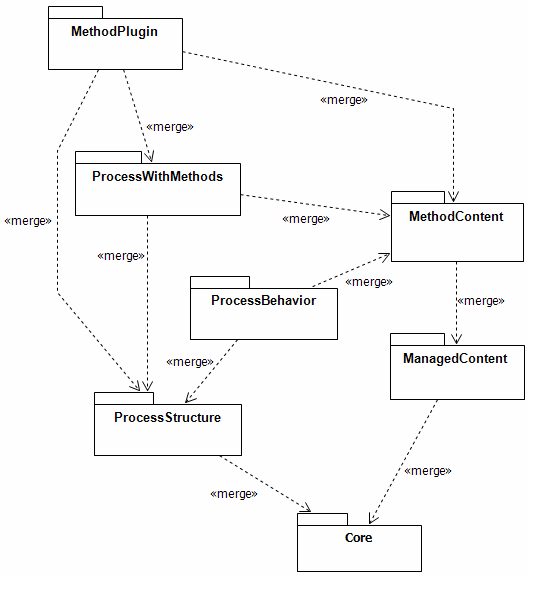
\includegraphics[scale=0.5]{./img/spem20.png}
 % matrixargseg.png: 296x162 pixel, 100dpi, 7.52x4.11 cm, bb=0 0 213 117
 %\caption{Estágio desenvolvimento de jogos ~\cite{fullerton2008game}}
\caption{Estrutura do meta-modelo SPEM 2.0}
%  \caption{Estágio desenvolvimento de jogos}
 \label{fig:spem20}
\end{figure}

Esse processo foi modelado a partir da ferramenta \ac{epf} \cite{epf13}, essa ferramenta é utilizada para autoria de processos através da notação de descrição de processos \ac{spem} \cite{spem08}. A partir dela é possível criar, customizar e publicar os processos de desenvolvimento.

\section{Visão Geral}
O processo proposto, chamado \textbf{GAme Health Monitor Embedded-UFCG Process} (\textit{GAHME Process}), aborda o desenvolvimento componente de software para jogos eletrônicos, com o objetivo monitorar dados de saúde. 

Com o desenvolvimento da proposta, procuramos criar um processo que fosse genérico o suficiente para atender diversos tipos de jogos, mas que contemplasse a capacidade de monitoramento dos dados de modo que o jogo pudesse: capturar dados de saúde, identificar sintomas e validar a proposta do jogo com a ocorrência dos sintomas a serem monitorados. Desta forma, podemos dizer que a principal contribuição deste processo é fornecer um conjunto coerente de atividades e artefatos direcionados para o Desenvolvimento de Jogos Com a Capacidade de Monitorar Dados de Saúde, mas que mantém a generalidade de um processo de desenvolvimento de software podendo ser aplicado no contexto de desenvolvimento de jogos.

\begin{figure}
 \centering
 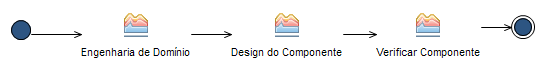
\includegraphics[scale=0.8]{./img/visaogeral.png}
 % matrixargseg.png: 296x162 pixel, 100dpi, 7.52x4.11 cm, bb=0 0 213 117
 %\caption{Estágio desenvolvimento de jogos ~\cite{fullerton2008game}}
\caption{Visão Geral \textit{\ac{gahme} Process}}
%  \caption{Estágio desenvolvimento de jogos}
 \label{fig:visaogeral}
\end{figure}

\begin{figure}
 \centering
 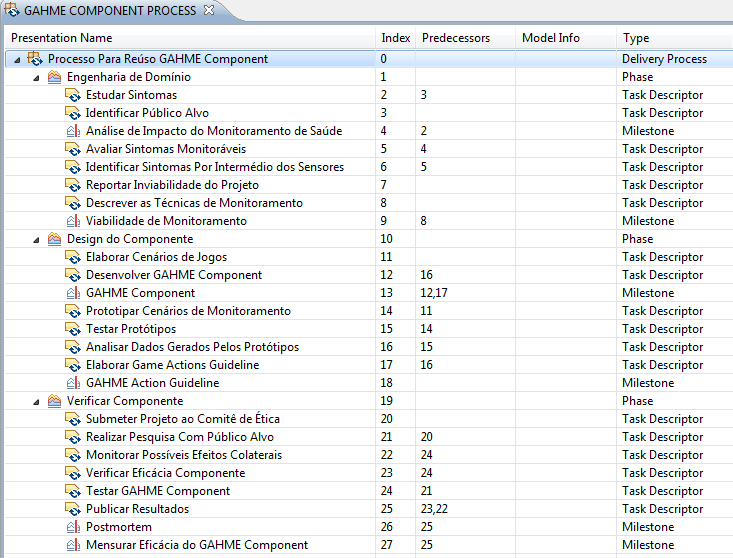
\includegraphics[scale=0.8]{./img/wbs2.png}
 % matrixargseg.png: 296x162 pixel, 100dpi, 7.52x4.11 cm, bb=0 0 213 117
 %\caption{Estágio desenvolvimento de jogos ~\cite{fullerton2008game}}
\caption{Estrutura Analítica do Processo Para Reúso \ac{gahme} Component}
%  \caption{Estágio desenvolvimento de jogos}
 \label{fig:visaogeral}
\end{figure}

\section{Papéis e Responsabilidades}
%Nesta seção serão descritoos os papéis previstos no processo, bem como a descrição de suas principais habilidades e atribuições.

O \textit{GAHME Process} é um processo de jogos eletrônicos que permitem realizar o monitoramento de dados de saúde, a descrição dos papéis presentes no processo se faz importante para um melhor entendimento das atividades realizadas em cada fase do processo.

\subsection{\textit{Game Designer}}\label{subsec:game_designer}
O projeto de um jogo eletrônico requer a contribuição de diversos perfis e habilidades. O \textit{Game Designer} deve trabalhar em colaboração com todos os membros da equipe de desenvolvimento como Engenheiro de Software, \textit{Art Designer} e conhecer também o que o jogador espera encontrar em um jogo ~\cite{schell2008art}. Um bom \textit{Game Designer} está disposto a escutar as diferentes opiniões e sugestões e selecionar aquelas que venham melhorar a experiência do jogo ~\cite{moore2011basics}. Esse papel é responsável pela concepção do jogo, passando por atividades de análise, melhoramento do documento e verificação do resultado final do jogo.

\subsubsection{Habilidades}
Para desempenhar este papel é necessário que o integrante tenha o perfil com as seguintes habilidades:
  \begin{itemize}
	  \item Entender dos anseios e ponto de vista do jogador em relação ao jogo a ser desenvolvido ~\cite{schell2008art};
		\item compreender as ações monitoráveis que o jogador poderá executar definidos no \textit{Game Actions Design} (Seção \ref{subsec:game_actions_guide});
		\item conceber o jogo o que confere a narrativa, regras e objetivos do jogo ~\cite{schell2008art,moore2011basics,bethke2003game}
  \end{itemize}

\subsubsection{Abordagens de Atribuição}
O \textit{Game Designer} deve ter conhecimento sobre as capacidades técnicas da equipe e da \textit{engine} de jogos selecionada para o desenvolvimento do jogo. É essencial que o \textit{Game Designer} conheça sobre as ações que os jogadores precisem desempenhar para serem monitorados. Essa habilidade poderá ser obtida através do \textit{GAHME Actions Guideline}, que conterá a descrição dessas ações.

\subsection{\textit{Game Health Designer}}
O \textit{Game Health Designer} tem um papel bem parecido com o do \textit{Game Designer} (Seção \ref{subsec:game_actions_guide}) contudo deverá trabalhar em colaboração maior com o Profissional de Saúde e do Engenheiro de Software na fase de \textit{Iniciação} onde serão verificadas a viabilidade de um jogo com objetivo de monitoramento de saúde e na elaboração do \textit{Game Actions Design} (\ref{subsec:game_actions_guide}) artefato que fará um mapeamento das ações passíveis de monitoramento e sua relação com os dados de saúde que serão monitorados durante o jogo. Esse último artefato, deverá ser utilizado pelo \textit{Game Designer} para a elaboração do enredo e cenários do jogo.

\subsubsection{Habilidades}
Para desempenhar este papel é necessário que o integrante tenha o perfil com as seguintes habilidades:
  \begin{itemize}
	  \item Compreender as diretrizes médicas (Seção \ref{subsec:diretrizes_medicas}) e conseguir extrair sintomas monitoráveis com o auxílio do Profissional de Saúde;
		\item analisar as possibilidades de monitoramento por intermédio dos sensores disponíveis e com o auxílio do Engenheiro de Software que irá verificar a viabilidade do monitoramento;
		\item verificar a viabilidade do monitoramento dos dados de saúde por intermédio de um jogo eletrônico;
		\item conceber um artefato de \textit{Game Actions Design} que auxilie na concepção do jogo por parte do \textit{Game Design}.
  \end{itemize}

\subsubsection{Abordagens de Atribuição}
O \textit{Game Health Designer} deve ter conhecimento tanto da área de saúde quanto das tecnologias utilizadas no desenvolvimento dos jogos.


% In the last few months of production, the focus shifts from producing new code and features to making certain that what has already been built functions as expected and that the levels and artwork are complete and polished. The team shrinks down in size because the majority of production artists and outside talent such as sound designers and writers are no longer needed ~\cite{fullerton2008game}.


\section{Fase: Engenharia de Domínio}
O objetivo da iteração de Engenharia de Domínio é identificar o impacto que o jogo para o monitoramento de dados de saúde trará e avaliar se será possível desenvolver esse jogo com a tecnologia atual.

\begin{figure}
 \centering
 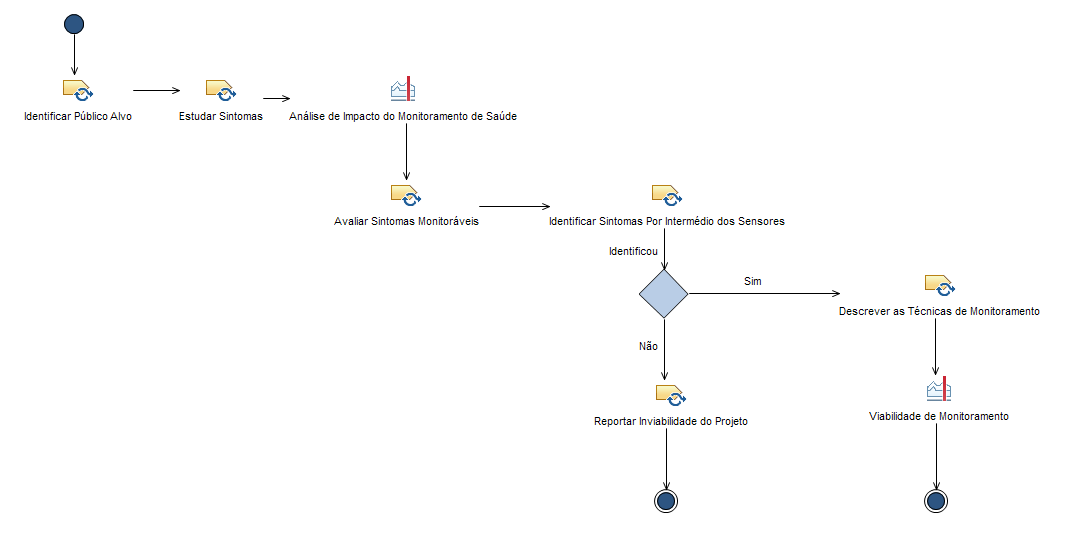
\includegraphics[scale=0.55]{./img/engenhariadominio.png}
 % matrixargseg.png: 296x162 pixel, 100dpi, 7.52x4.11 cm, bb=0 0 213 117
 %\caption{Estágio desenvolvimento de jogos ~\cite{fullerton2008game}}
\caption{Fase: Engenharia de Domínio do \textit{GAHME Process} Orientado à Reúso}
%  \caption{Estágio desenvolvimento de jogos}
 \label{fig:iniciacao}
\end{figure}

\subsection{Atividade: Identificar Público Alvo}
Primeiramente o \textit{Game Health Designer} deverá encontrar qual é o perfil do jogador, essa é uma questão importante, pois irá definir o público alvo do jogo. Se será destinado a um público que já possui o hábito de jogar jogos eletrônicos ou a um público com um nível de habilidade menor. Se haverá sistema de balanceamento de dificuldades tentando atender os dois públicos ~\cite{brathwaite2009challenges}. É necessário também avaliar a faixa etária a que se destina o jogo, pois jogos desenvolvidos para um público infantil tem um perfil bastante diferente dos voltados para adultos ~\cite{brathwaite2009challenges}, e isso irá impactar diretamente na elaboração do \texit{Game Design} do projeto, pois deve-ser levado em consideração que as crianças preferem ambientes mais lúdicos ~\cite{yannakakis06}, e pessoas idosas devem e precisam de jogos não os ponha em situação de risco de saúde como quedas ou fadiga muscular ~\cite{brox11,arntzen2011}.
Para a execução desta atividade o \textit{Game Health Designer} deverá fazer uso do Documento de Diretrizes Médicas (Seção \ref{subsec:diretrizes_medicas}) para identificar a necessidade de monitoramento dos sintomas, juntamente com o Profissional de Saúde, deverão selecionar sintomas que identifique problemas de saúde e que sejam mensuráveis por intermédio de sensores. Durante a execução desta atividade também deve ser coletado as informações a respeito da importância, impactos e benefícios ao tratamento de saúde o público alvo terá ao ter esses sintomas monitorados.

\subsubsection{Papéis Responsáveis}
\begin{itemize}
	\item \textit{Game Health Designer};
	\item Profissional de Saúde.
\end{itemize}

\subsubsection{Passos para Execução da Atividade}
\begin{itemize}
	\item Avaliar faixa etária;
	\item avaliar necessidade de monitoramento;
	\item avaliar sintomas a ser monitorados.
\end{itemize}

\subsubsection{Artefatos de Entrada}
\begin{itemize}
	\item Diretrizes Médicas.
\end{itemize}

\subsubsection{Artefatos de Saída}
\begin{itemize}
	\item Documento de Análise de Impacto.
\end{itemize}


\subsection{Atividade: Estudar Sintomas}
O objetivo principal dessa atividade é identificar sintomas passíveis de monitoramento por meio das Diretrizes Médicas que servirão de base científica para a execução desta atividade. Nessa atividade não deve ser levada em consideração a existência ou especificações técnicas dos sensores, isso será realizado posteriormente na atividade de Viabilidade do Monitoramento. O estudo dos sintomas será baseado nas diretrizes médicas, por meio destas o \textit{Game Health Design} irá mapear os sintomas e valores que identifiquem a sua ocorrência.
%No artefato de saída dessa atividade (Documento de Sintomas Passíveis de Monitoramento) deverão estar presentes os sintomas e possíveis valores para cada sintoma coletado.

\subsubsection{Papéis Responsáveis}
\begin{itemize}
	\item \textit{Game Health Designer};
	\item Profissional de Saúde.
\end{itemize}

\subsubsection{Passos para Execução da Atividade}
\begin{itemize}
	\item Estudar sintomas monitoráveis;
	\item Descrever sintomas passíveis de monitoramento;
	%\item Especificar valores que identifiquem os sintomas;	
\end{itemize}

\subsubsection{Artefatos de Entrada}
\begin{itemize}
	\item Diretrizes Médicas.
\end{itemize}

\subsubsection{Artefatos de Saída}
\begin{itemize}
	\item Documento de Sintomas Passíveis de Monitoramento.
\end{itemize}


\subsection{Atividade: Pesquisar População Beneficiada}
\subsubsection{Papéis Responsáveis}
\begin{itemize}
	\item \textit{Game Health Designer};
	\item Profissional de Saúde.
\end{itemize}

\subsubsection{Passos para Execução da Atividade}
\begin{itemize}
	\item Identificar público alvo
	\item 
\end{itemize}

\subsubsection{Artefatos de Entrada}
\begin{itemize}
	\item Diretrizes Médicas.
\end{itemize}

\subsubsection{Artefatos de Saída}
\begin{itemize}
	\item Documento de Sintomas Passíveis de Monitoramento.
\end{itemize}

\section{Fase: Verificar Componente}
Nos últimos anos houve um crescimento de jogos voltados para saúde, contudo muito desses jogos não foram validados efetivamente ou foi realizado um estudo para verificar os seus resultados ~\cite{kato12}. Os estudos realizados por muitos desses jogos, foram mal projetados e suas conclusões não podem se consideradas validas ou eficazes. Por esse motivo Kato ~\cite{kato12}, sugeriu diretrizes para a realização de estudos de eficácia para ser aplicados em jogos para saúde. 
Como a iteração de "Verificação" é responsável por avaliar a eficácia do monitoramento dos dados de saúde a partir do jogo desenvolvido, as sugestões definidas por Kato ~\cite{kato12} estarão presentes no decorrer da iteração.

Para Kato ~\cite{kato12}, os jogos para saúde precisam passar por pesquisa entre seres humanos e testado com grupo de controle para verificar sua eficácia. Deste modo, os jogos para monitoramento de saúde devem ser submetidos a testes com usuários para verificar se os sinais dos jogadores estão sendo capturados corretamente durante a execução de uma partida. Com o sucesso da execução desta etapa pode ser afirmado que foi desenvolvido um jogo com o propósito de monitoramento de dados de saúde.

\begin{figure}
 \centering
 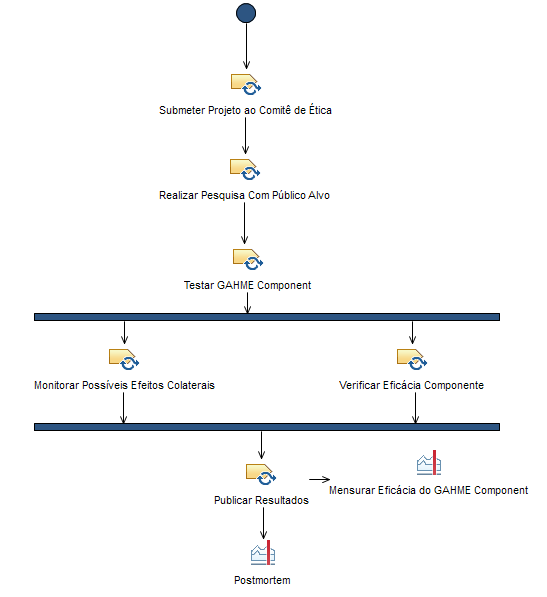
\includegraphics[scale=0.55]{./img/verificar-componente.png}
 % matrixargseg.png: 296x162 pixel, 100dpi, 7.52x4.11 cm, bb=0 0 213 117
 %\caption{Estágio desenvolvimento de jogos ~\cite{fullerton2008game}}
\caption{Iteração: Verificação do \textit{GAHME Process}}
%  \caption{Estágio desenvolvimento de jogos}
 \label{fig:verificação}
\end{figure}

\subsection{Submeter Projeto ao Comitê de Ética}
O objetivo dessa atividade é submeter o jogo às normas regulamentadoras previstas para a pesquisa envolvendo seres humanos segundo a Resolução 196/96 ~\cite{conselho2000normas}. Segundo o Conselho Nacional de Saúde ~\cite{conep2002}, o \ac{cep} é um colegiado interdisciplinar e independente,  que deve existir nas instituições que realizam pesquisas envolvendo seres humanos no Brasil, criado para defender os interesses dos sujeitos da pesquisa em sua integridade e dignidade e para contribuir no desenvolvimento da pesquisa dentro de padrões éticos (Normas e Diretrizes Regulamentadoras da Pesquisa Envolvendo Seres Humanos - Res. CNS 196/96 ~\cite{conselho2000normas}). 

O \ac{cep} é responsável pela avaliação e acompanhamento dos aspectos éticos de todas as pesquisas envolvendo seres humanos. Este papel está bem estabelecido nas diversas diretrizes éticas internacionais (Declaração de Helsinque, Diretrizes Internacionais para as Pesquisas Biomédicas envolvendo Seres Humanos – CIOMS) e Brasileiras (Res. CNS 196/96 e complementares~\cite{conselho2000normas}), diretrizes estas que ressaltam a necessidade de revisão ética e científica das pesquisas envolvendo seres humanos, visando a salvaguardar a dignidade, os direitos, a segurança e o bem-estar do sujeito da pesquisa ~\cite{conep2002}.

Nessa atividade deve ser elaborado um Protocolo de Pesquisa, contemplando a descrição da pesquisa, estabelecer critérios de inclusão e exclusão dos sujeitos da pesquisa, a qualificação dos pesquisadores e todas instâncias responsáveis pelo projeto. Devem fazer presentes no projeto Instituições de pesquisa, legitimamente constituída e habilitada que permita realizar as investigações científicas. 

Os pesquisadores, deverão elencar os riscos da pesquisa, principalmente danos físicos, psíquicos, moral, intelectual, cultural do ser humano em qualquer fase de uma pesquisa dela decorrente ~\cite{conselho2000normas}. Sendo necessária a anuência do sujeito da pesquisa ou de um representante por intermédio do Consentimento livre e esclarecido, onde será explicado a natureza da pesquisa, seus objetivos, métodos, benefícios previstos, potenciais riscos e o incômodo que esta possa acarretar, formulada em um termo de consentimento, autorizando sua participação voluntária na pesquisa ~\cite{conselho2000normas}. Caso o sujeito da pesquisa se enquadre nos critérios estabelecidos para interromper a pesquisa, essa deverá ser finalizada assegurando a integridade do mesmo.

Atualmente no Brasil para poder testar o jogo com monitoramento de dados de saúde junto a pacientes e testar de fato a eficácia do jogo é necessário passar por esse processo e obter a aprovação de um \ac{cep}. Esse é um processo demorado e pode impactar bastante a entrega final.


\subsection{Realizar Pesquisa com Público Alvo}
Durante a pesquisa com o público alvo, o pesquisador deverá ter a preocupação com a integridade do sujeito da pesquisa.
Para isso deverá obedecer o que ficou definido nos "Critérios Para Interromper a Pesquisa" no projeto aprovado pelo \ac{cep}. Segundo a Resolução 196/96 ~\cite{conselho2000normas} caso o pesquisador identifique risco ou dano à saúde do sujeito participante da pesquisa e que não esteja presente no termo de consentimento, o pesquisador é obrigado a suspender a pesquisa. Do mesmo modo, caso haja um método mais seguro para realizar a pesquisa, o projeto deverá ser suspenso, oferecendo a todos os sujeitos os benefícios do melhor regime ~\cite{conselho2000normas}.

Na seção de Riscos e Benefícios da Resolução 196/96 ~\cite{conselho2000normas}, fica fadado ao pesquisador,patrocinador e a instituição devem assumir a responsabilidade de dar assistência integral às complicações e danos decorrentes dos riscos previstos. Os sujeitos da pesquisa que vierem a sofrer qualquer tipo de dano previsto ou não no termo de consentimento e resultante de sua participação, além do direito à assistência integral, têm direito à indenização. Jamais poderá ser exigido do sujeito da pesquisa, sob qualquer argumento, renúncia ao direito à indenização por dano. O formulário do consentimento livre e esclarecido não deve conter nenhuma ressalva que afaste essa responsabilidade ou que implique ao sujeito da pesquisa abrir mão de seus direitos legais, incluindo o direito de procurar obter indenização por danos eventuais.

\subsection{Monitorar Possíveis Efeitos Colaterais}
Durante a execução da pesquisa possíveis efeitos colaterais devem ser monitorados como: risco de queda, fadiga, tendinite. 
s avaliações de jogos para a saúde devem tentar controlar o uso de seu jogo para efeitos colaterais negativos. possível negativo efeitos colaterais dos jogos, embora rara, pode incluir convulsões, devido à fotossensibilidade e tendinites.

\subsection{Verificar Eficácia do Jogo}
A eficácia do jogo será verificada através de um estudo analítico de caso-controle ~\cite{menezes2001epidemiologia}, dentro de um ambiente aprovado pelo \ac{cep} que permitirá recrutar sujeitos de pesquisa. Uns sujeitos deverão apresentar os sintomas a serem monitorados e outros não terão tais sintomas. Os dados serão coletados e ao final deverá ser verificado se os sintomas foram corretamente identificados.

Kato ~\cite{kato12}, defende que para essa verificação é necessário obter um número adequado de participantes para conseguir avaliar o impacto do jogo. Contudo, determinados sintomas possuem poucos sujeitos de pesquisa disponíveis reduzindo a abrangência da pesquisa.

Em uma revisão sistemática sobre a eficácia dos jogos existes e que promovem a atividade física para adolescentes ~\cite{foley-active-game2010}, segundo a revisão a abordagem de jogos se mostrou eficaz ao motivar a execução de atividade física dos usuários. Os jogos estudaram envolveram tanto os membros superiores quanto inferiores do corpo melhorando a atividade de forma prazerosa e com qualidade inclusive em grupos de deficiência e de alto risco.

%Verificar essa referencia ~\cite{Primack2012630}

\subsection{Publicar Resultados}
\section{Artefatos}

Os documentos para o desenvolvimento de jogos tem dois propósitos principais: histórico do projeto e comunicação ~\cite{schell2008art}. O desenvolvimento de um jogo requer a tomada de decisões a todo o momento, que definem o funcionamento do jogo. Contudo, existe uma grande probabilidade de que os envolvidos do projeto não se recordem dos motivos que as decisões forma tomadas. Se a equipe de desenvolvimento tiver o hábito de armazenar todas as tomadas de decisões e documentá-las nos artefatos utilizados no desenvolvimento do software então não será necessário rediscutir as decisões já tomadas ~\cite{schell2008art}.
Os artefatos de software são importantes para comunicar sobre as decisões tomadas durante a concepção do projeto a todos os participantes do mesmo. É importante salientar que em um processo de software os artefatos servem como documentos de entrada e saída da execução de atividades dentro do próprio processo ~\cite{sommerville2011}.

\subsection{Diretrizes Médicas}\label{subsec:diretrizes_medicas}
O principal propósito da atividade médica é o cuidado do paciente, e isso traz enormes desafios de forma coletiva ou individual. Com o intuito de auxiliar na tomada de decisões, a comunidade médica mundial tem elaborado e divulgado um extenso número de informações ~\cite{nhs2013,neozeland-guide-2013}, muito mais acessíveis do que era no passado, redefinindo o universo do conhecimento médico, tornando-o livre e acessível para críticas e demais propósitos científicos ~\cite{proj-diretriz2013}.

Neste contexto, a Associação Médica Brasileira e o Conselho Federal de Medicina, também com o objetivo de auxiliar na decisão médica e, consequentemente, otimizar o cuidado aos pacientes, desencadearam um processo junto às Sociedades de Especialidade para a elaboração de Diretrizes Médicas baseadas nas evidências científicas disponíveis na atualidade ~\cite{proj-diretriz2013}.
Nesse processo, formou-se por uma Comissão Técnica responsável em construir as bases de sustentação das recomendações de conduta médica, utilizando os meios da ciência atual, de forma crítica e desprovida de interesse se não aquele que resulte na melhoria do tratamento do médico com o paciente. 

Partindo do princípio que o conhecimento médico atual está presente nas diretrizes médicas e que através do seu conteúdo é possível 	extrair informações que permitam identificar e avaliar a presença e evolução de sintomas de doenças, esse artefato será de extrema importância para o desenvolvimento de um jogo eletrônico com o objetivo de realizar o monitoramento de dados de saúde.
%Nas diretrizes médicas estão descritos mecanismos de diagnósticos, prognóstico, tratamento, dosagem medicamentosa, riscos e benefícios. Além de definir questões mais relacionadas à prática clínica e descrevendo as possíveis opções para a tomada de decisão sobre o tratamento da doença .a ser monitorada como por exemplo a Doença de Parkinson que servirá como estudo de caso do presente trabalho ~\cite{protpar010}.
%evidências através dos dados sobre a doença bem como mecanismos de diagnósticos, prognóstico, tratamento, dosagem medicamentosa, riscos e benefícios. Além de definir questões mais relacionadas à prática clínica e descrevendo as possíveis opções para a tomada de decisão sobre o tratamento da doença .a ser monitorada como por exemplo a Doença de Parkinson que servirá como estudo de caso do presente trabalho ~\cite{protpar010}.
\subsubsection{Propósito}
As diretrizes médicas permitem identificar sintomas passíveis de monitoramento, bem como parâmetros  relevantes a esses sintomas. As diretrizes médicas são documentos produzidos por sólidas bases científicas, sendo escrita pela própria comunidade médica que determina seus representantes. Por esse motivo, esse documento passa por rigorosas revisões e em constantes atualizações, sendo uma das principais referências para os profissionais da saúde. Para o \textit{GAHME Process} este artefato servirá de base científica para fundamentar quais sintomas serão monitorados e de que forma serão avaliados.


%\subsection{Estudos Epidemiológicos}\label{subsec:estudos_epidemiologicos}
%A Epidemiologia é a ciência que estuda ocorrência de doenças em populações humanas e seus fatores determinantes das doenças ou condições relacionadas à saúde em populações especificadas no estudo ~\cite{menezes2001epidemiologia,lima-costa-2003}. Inicialmente a epidemiologia restringia-se a estudo de epidemias de doenças transmissíveis, contudo atualmente a epidemiologia trata qualquer evento relacionado à saúde (ou doença) da população ~\cite{menezes2001epidemiologia}.
%
%%\subsubsection{Tipos de Estudos epidemiológicos}
%Os estudos epidemiológicos podem ser classificados em observacionais e experimentais, para o este trabalho serão utilizados estudos epidemiológicos observacionais descritivos têm por objetivo determinar a distribuição de doenças ou condições relacionadas à saúde, segundo o tempo, o lugar e/ou as características dos indivíduos ~\cite{lima-costa-2003}. Ou seja, responder à pergunta: quando, onde e quem adoece? Logo, as respostas dessas perguntas serão fundamentais para avaliar o impacto de possíveis tratamentos, medicamentos trabalho ou em nosso caso do desenvolvimento de um jogo que permita o monitoramento de dados de saúde.
%
%A epidemiologia descritiva pode fazer uso de dados secundários (dados pré-existentes de mortalidade e hospitalizações, por exemplo) e primários (dados coletados para o desenvolvimento do estudo) ~\cite{lima-costa-2003}. No Brasil, existem importantes bancos de dados secundários com abrangência nacional que podem ser usados para estudo epidemiológicos como: Sistema de Informações sobre Mortalidade (SIM-SUS) ~\cite{sis2013}, Pesquisa Nacional de Amostra Domiciliar (PNAD) ~\cite{pnad2008} bem como os estudos epidemiológicos realizados no Brasil e disponibilizados em Bases de estudo em saúde como Scielo ~\cite{scielo2013}.

%\subsubsection{Propósito}
%O propósito deste artefato é identificar a população beneficiada como o monitoramento dos dados de saúde por intermédio dos jogos eletrônicos.

\subsection{Documento de Sintomas Passíveis de Monitoramento}
Baseado nas Diretrizes Médicas (Seção \ref{subsec:diretrizes_medicas}) e na Especificação dos Sensores existentes o \textit{GAHME Designer} irá identificar e descrever quais sintomas são passíveis de monitoramento. Para a elaboração deste artefato faz-se necessária a colaboração do Engenheiro de Software devido a seu perfil tecnológico e este entender as especificação do sensor. Como também, do Profissional de Saúde para definir qual sintoma deve ser monitorado e como esse monitoramento deve ser realizado.

É de extrema importância que o \textit{Game Health Designer} participe das discussões tanto de saúde quanto tecnológicas, pois ele é que irá conceber as ações realizadas pelo Jogador durante o jogo, logo ele deverá saber tanto das limitações técnicas dos sensores quanto os movimentos que o jogador deverá efetuar quando estiver jogando. Esse artefato é o \textit{milestone} da fase de \textit{Iniciação}, será através dele que será decidida a viabilidade do desenvolvimento do jogo nas fases seguintes do processo de desenvolvimento. Contudo, mesmo sendo um artefato elaborado na primeira fase do desenvolvimento do jogo (Iniciação), este não será descartado nas demais fases de desenvolvimento. Pois este servirá como entrada para a elaboração do \textit{GAHME Actions Guideline} (Seção \ref{subsec:game_actions_guide}) que conterá as ações monitoráveis dos jogadores.

\subsection{Cenário de Jogo}
A fase de concepção do cenário do jogo para muito autores é definida como crucial para conseguir um jogo de sucessos e atingir elementos difíceis de ser mensurados como por exemplo a diversão. É sabido que a utilização de protótipos nas etapas iniciais do processo de desenvolvimento permitem anteceder o comportamento do jogo e auxiliar na definição do mesmo durante a elaboração do \textit{Game Design}, pois os jogadores poderão ter uma noção da experiência do jogo nas etapas iniciais e permitirão que estes possam tecer seus comentários livremente e sugerir modificações ~\cite{prototipgames2007}.
 
Para conceber os cenários iniciais, não precisa necessariamente desenvolver um jogo para esse propósito. Estudos indicam que mecanismos de prototipagem rápida ou de baixo custo ~\cite{prototipgames2007,fullerton2008game} permitem o entendimento da ideia proposta e habilita aos participantes da discussões propor sugestões que venham melhorar a proposta logo no início reduzindo o custo com modificações em fases mais adiantadas do desenvolvimento. Fullerton ~\cite{fullerton2008game}, defende que a prototipação física permite que os participante se concentrem nos mecanismos do jogo sem se preocupar com os aspectos tecnológicos do mesmo, possibilitando que membros da equipe que não tem perfil técnico possam mostrar sua perspectiva e consequentemente contribuir no \textit{game design}. Como pode ser visto na Figura \ref{fig:proto-fps}um exemplo de protótipo físico de um cenário de jogo de um FPS, essa abordagem permite a compreensão sobre a estratégia do jogo, visualização de possíveis cenários e até mesmo a alteração do mesmo de forma rápida, contrastando com a dificuldade de alterar um ambiente 3D digital ~\cite{fullerton2008game}. 

\begin{figure}
 \centering
 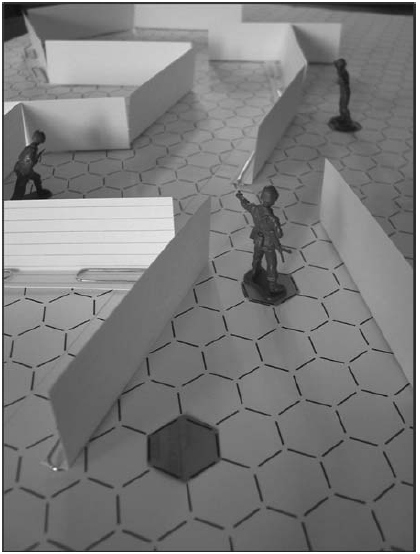
\includegraphics[scale=0.55]{./img/fps-fisical-prototype.png}
 % matrixargseg.png: 296x162 pixel, 100dpi, 7.52x4.11 cm, bb=0 0 213 117
 %\caption{Estágio desenvolvimento de jogos ~\cite{fullerton2008game}}
\caption{Prototipação Física de um \ac{fps} ~\cite{fullerton2008game}}
%  \caption{Estágio desenvolvimento de jogos}
 \label{fig:proto-fps}
\end{figure}

%Uma das etapas do planejamento do designer passa pela concretização da suas ideias através de modelos que consigam certificar de que a concepção é realmente divertida e através de protótipos será possível demonstrá-la para os demais membros da equipe, garantindo que será dada continuidade ao projeto para a produção definitiva ~\cite{prototipgames2007}. Os benefícios do uso de protótipos rápidos é que ele permite testes rápidos de componentes separadamente sem necessariamente implementar o sistema completo como também encoraja usuários a comentar livremente e sugerir modificações (contrário a um produto bem acabado que pode parecer já terminado). Porém, como ponto negativo, temos muitas vezes componentes individuais devem ser re-testados no produto finalizado ~\cite{prototipgames2007}.


%
%
%
%
%\subsection{Protótipo Jogável}
%Game prototypes, while playable, usually include only a rough approximation of the artwork, sound, and features. They are very much like sketches whose purpose is to allow you to focus on a small set of the game’s ~\cite{fullerton2008game}. There are many types of prototypes, including physical prototypes, visual prototypes, video prototypes, software prototypes, etc. 
%
%Prototyping lies at the heart of good game design. Prototyping is the creation of a working model of your idea that allows you to test its feasibility and make improvements to it ~\cite{fullerton2008game}. 
%
%%Buskirk e Moroney [2003] afirmam que o uso da técnica de prototipagem pode ser estendido para outras fases do ciclo de vida do produto além dos testes de usabilidade. Sendo usado na validação dos requisitos junto aos consumidores, na fase de especificação do projeto, desenvolvimento dos manuais do produto, suporte ao marketing, execução de testes funcionais, ajuda no serviço de atendimento aos clientes ~\cite{prototipgames2007}.O público-alvo dessa avaliação inicial inclui publishers, engenheiros de software, artistas, e outros membros da equipe. Como “palavras são fundamentalmente uma maneira terrível de comunicar interatividade” [Waugh 2006], podemos tomar o desenvolvimento de protótipos como meio para ajudar a educar a equipe de como alguns componentes do jogo deveriam se comportar, esclarecendo de forma mais amigável os conceitos abstratos e poder transmitir como o jogo deve funcionar ~\cite{prototipgames2007}.
%If you try to design the entire game at once, you might become confused and overwhelmed. There are so many elements in a typical game that it is diffi cult to know where and how to start. What we recommend is that you isolate the core gameplay mechanisms and build out from there ~\cite{fullerton2008game}.
%
%
%
%\subsection{GAHME Actions Guideline}\label{subsec:game_actions_guide}
%
%Para elaboração deste artefato o \textit{Game Health Designer}, utilizará como irá utilizar as Diretrizes Médicas como base científica de conhecimento e das especificações dos sensores de captura que poderão ser utilizados.
%
%Para elaboração deste artefato o 
%
%Para a sua elaboração o responsável Os artefatos de entrada para elaboração
%
%O responsável pela elaboração do GAHME Actions Design é o que deverá se basear nas Diretrizes Médicas, para fazer uma avaliação dos mPara elaboração do GAHME Actions Design, o autor 
%
%Nesse artefato é levado em consideração o sensor utilizado, o sintoma a ser monitorado e a eficácia do monitoramento sendo comprovada por intermédio de testes efetuados na atividade \textit{Testar Protótipos} da fase de \textit{Prototipação}.
%
%The core gameplay mechanism, or “coremechanic,” can be defi ned as the actions that a player repeats most o en while striving to achieve the game’s overall goal. Games are repetitive by nature. While the meaning and consequences of what a player does can change over the course of game, the core actions tend to remain the same from beginning to end ~\cite{fullerton2008game}.
%
%Creating a physical prototype is a critical step in the design of your original game concept. It will save your team tremendous amounts of time because everyone will have a clear understanding of the game you are making. In addition, a physical prototype will enable you to focus your creative energy on the game mechanics without becoming distracted by the production and programming process ~\cite{fullerton2008game}. 
%
%
%
%\subsection{GAHME Actions Design}
%O objetivo deste artefato é definir quais são os movimentos efetuados pelo jogador dentro do jogo que são passíveis de monitoramento. Para elaboração deste artefato o \textit{GAHME Designer}, irá utilizar as Diretrizes Médicas como base científica de conhecimento e das especificações dos sensores de captura que poderão ser utilizados.
%
%Por promover atividades físicas, ou ações que possam trazer injúria ao jogador, como movimentos de equilíbrio, movimentos repetitivos ou rápidos. O game design do jogo deve ter a preocupação de desenvolver o jogo de acordo com o público-alvo. Isso significa dizer que a faixa etária e limitações físicas e cognitivas em decorrência da idade ou enfermidade devem ser levadas em consideração. Os jogadores devem ter a segurança de usarem o jogo e ter a certeza que o seu uso não acarretará em injúria ~\cite{arntzen2011}.
%
%
%
%
%
%Para elaboração deste artefato o 
%
%Para a sua elaboração o responsável Os artefatos de entrada para elaboração
%
%O responsável pela elaboração do GAHME Actions Design é o que deverá se basear nas Diretrizes Médicas, para fazer uma avaliação dos mPara elaboração do GAHME Actions Design, o autor 
%
%Nesse artefato é levado em consideração o sensor utilizado, o sintoma a ser monitorado e a eficácia do monitoramento sendo comprovada por intermédio de testes efetuados na atividade \textit{Testar Protótipos} da fase de \textit{Prototipação}.
%




\chapter{Abordagem \textit{GAHME}}\label{chapter:abordagem_gahme}
A abordagem \textit{GAHME} é um modelo de monitoramento de dados motores de saúde por meio de jogos eletrônicos. Para essa abordagem tornar-se viável, é necessário primeiramente realizar um estudo sobre quais os movimentos e ações o usuário deve exercer para que os sinais motores sejam capturados corretamente e torne possível a identificação dos sintomas. De posse dos movimentos, estes devem ser testados junto a indivíduos portadores da deficiência a ser monitorada e indivíduos como grupo de controle para avaliar a detecção do sintoma.


\section{Definição de Requisitos da Solução}\label{section:requisitos_solucao}
Com base no levantamento bibliográfico e em entrevistas preliminares com profissionais de saúde, os seguintes requisitos funcionais foram definidos para a solução \textit{GAHME}:

\begin{description}
	\item[REQ-GAHME-01 - Pontuação e Taxa de Acerto]: O jogador percebe os objetivos e visualiza o sucesso ou fracasso alcançado. O jogo pontua o jogadora de acordo com seus seus erros e acertos~\cite{Suhonen:2008:SFE:1457199.1457204,sinclair07}.
	\item[REQ-GAHME-02 - Progresso e Evolução do Jogador e dos Desafios]: O jogador percebe seu progresso e evolução no jogo. Os desafios tonam-se mais complexos no decorrer do tempo ~\cite{Suhonen:2008:SFE:1457199.1457204}.
	\item[REQ-GAHME-03 - Estado de Fluxo]: Um dos grandes desafios de um jogo eletrônico é levar o usuário a um ``Estado de Fluxo'' ou escapismo passando a executar a atividade proposta pelo jogo de uma forma autotélica, ou seja o usuário não vislumbra um benefício imediato ou futuro ~\cite{sweetser2005-gameflow}. 
	\item[REQ-GAHME-04 - Preocupação com Integridade Física do Jogador]: Promover atividades físicas, ou ações que venham a trazer injúria ao jogador, como movimentos de equilíbrio, movimentos repetitivos ou bruscos ~\cite{sinclair07,arntzen2011}.
		\item[REQ-GAHME-05 - Captura e Armazenamento de Sinais Motores]: O jogo deve realizar a captura dos sinais motores do usuário usando sensores de movimento. Os dados capturados são enviados à um servidor para tornar possível o acompanhamento da saúde motora.
	\item[REQ-GAHME-06 - Mecanismo de Identificação de Sintomas Motores]: Baseados em algoritmos de aprendizagem de máquina o servidor acompanha todos os usuários do sistema e identifica qual deles está com distúrbio motor, em caso afirmativo envia-se a informação ao profissional de saúde.
	\item[REQ-GAHME-07 - Mecanismo de Visualização dos Parâmetros Motores do Usuário]: O profissional de saúde poderá visualizar os dados identificados pela máquina de aprendizagem para realizar a tomada de decisão sobre o estado de saúde do usuário.
\end{description}

\section{Visão geral da solução}

A abordagem \textit{GAHME} faz uso de jogos eletrônicos como interface de captura, tornando os usuários mais motivados a fornecer os dados motores, em comparação ao uso dos dispositivos vestíveis. Desta forma, o profissional de saúde poderá visualizar os dados motores capturados em um momento em que o usuário está descontraído sem a preocupação de estar participando de um exame motor. 

\begin{figure}[!htb]
     \centering
     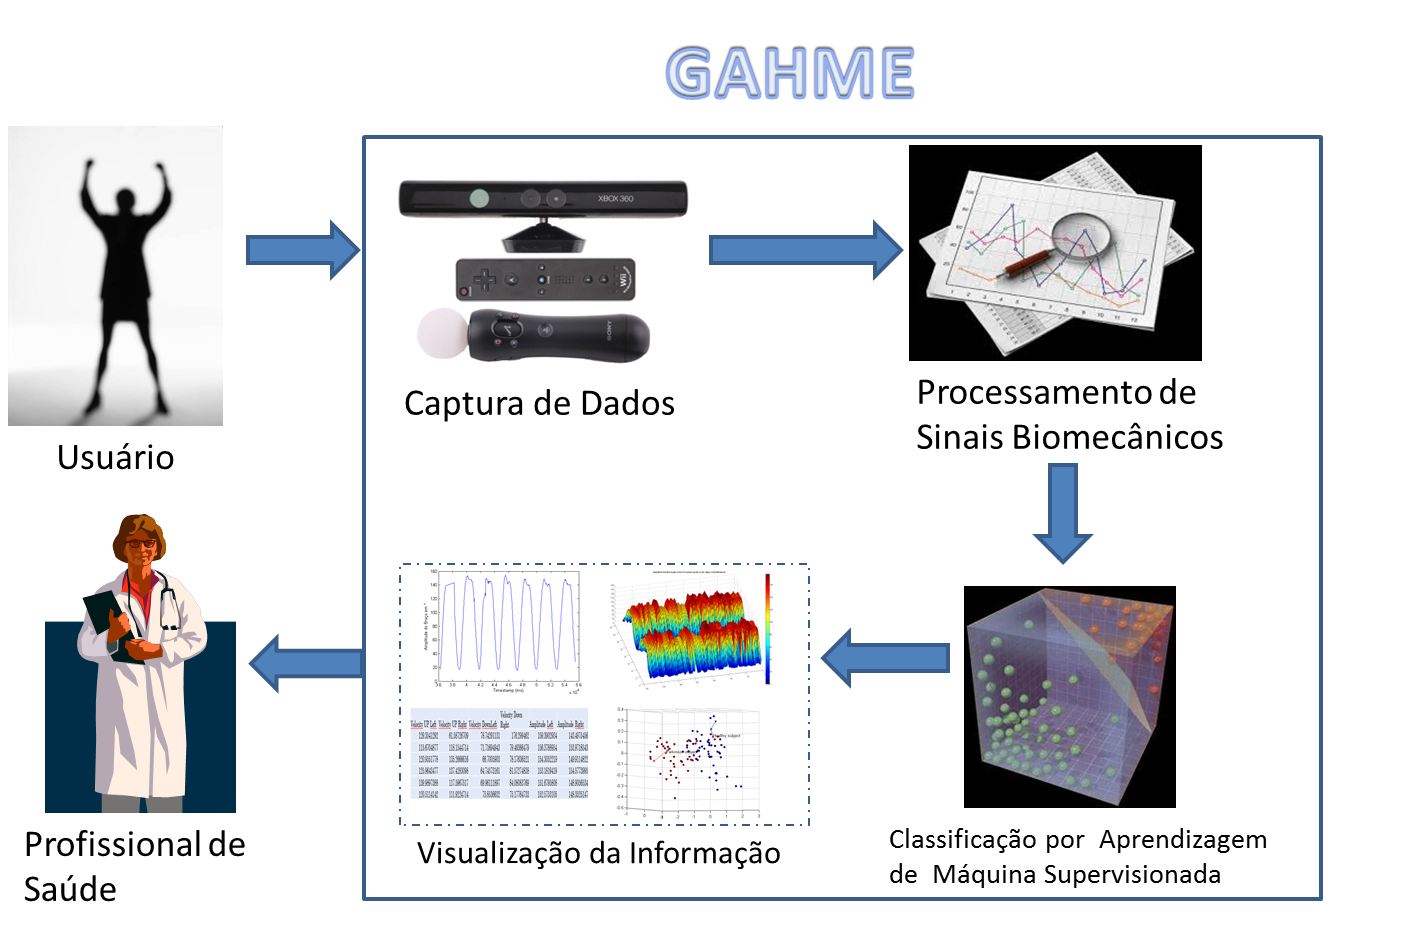
\includegraphics[width=1\textwidth]{./img/systemoverview.png}
     \caption{Visão Geral da Abordagem \textit{GAHME}}
     \label{img:visaogeral}
\end{figure}

Com o uso dos jogos eletrônicos é possível alcançar requisitos de pervasividade e não invasividade. Pois através dos dispositivos de sensores de movimento usados nesses ambientes, é possível desenvolver um jogo que motive o usuário a executar ações específicas que permitam o monitoramento de dados motores. A partir de uma interface com o usuário que permite enviar os dados capturados a um servidor, este fará o armazenamento dos dados para um possível acompanhamento da saúde motora.

Baseado em técnicas de processamento de sinais e reconhecimento de padrões, será possível identificar sintomas motores. Esta abordagem consiste em realizar o processamento dos dados com o objetivo de filtrar ciclos de movimento que permitam identificar sinais motores e como consequência seja possível extrair as características desse movimento. Após a extração das características, os dados são repassados para Máquinas de Aprendizagem que classificam os dados por meio das evidências estatísticas. Caso a máquina identifique algum usuário com distúrbio motor, ela poderá notificar o Profissional de Saúde e este poderá visualizar os dados para uma melhor tomada de decisão, como pode ilustrado na Figura~\ref{img:visaogeral}.

%A abordagem \textit{GAHME} pode ser vista como uma caixa preta que recebe como entrada os dados motores de indivíduos e tem como saída técnicas de aprendizagem de máquina para identificar a ocorrência sintomas motores. Caso a máquina de aprendizagem identifique algum problema motor em um indivíduo o Profissional de saúde poderá visualizar os dados e realizar a tomada de decisão sobre o tratamento.

%O Processamento de Sinais Biomecânicos e a Aprendizagem Supervisionada usam classificadores de dados. Esses módulos realizam o processamento dos dados com o objetivo de filtrar ciclos de movimento que possibilitem a identificação de sinais de motores de saúde e como consequência possam extrair as características desse movimento. Após a extração das características, os dados são repassados para Máquinas de Aprendizagem que classificam os dados por intermédio das evidências estatísticas encontradas neles como iremos explicar no decorrer deste capítulo.

O funcionamento da abordagem pode ser descrito como uma composição de quatro passos: captura dos sinais através de sensores, processamento de sinais biomecânicos, classificação dos dados e visualização.

\section{Aquisição de Dados}
O propósito de um \textit{GAHME} é coletar informações do estado motor dos indivíduos de forma não invasiva. Por este motivo, foi apresentada uma abordagem de jogos eletrônicos como infraestrutura de captura de dados motores por meio dos sensores de movimento utilizados.

O cliente \textit{GAHME} é um jogo com funcionalidades de aquisição de dados motores de movimentos específicos. Logo, ele realiza a captura e envio de dados para um servidor que recebe requisições para efetuar o recebimento e armazenamento das informações. Tornando possível armazenar o histórico do usuário para um acompanhamento dos sinais motores por um longo período. Desta maneira um profissional de saúde poderá visualizar a evolução da saúde motora do usuário.

\section{Processamento de Dados Biomecânicos}\label{sec:processador_bio}
O módulo de Processamento de Dados Biomecânicos é responsável por: filtrar, remover ruídos e identificar ciclos de movimento para uma posterior extração dos vetores de características. A partir dos dados processados, aplicam-se técnicas de aprendizagem de máquina para obter a classificação dos dados e consequentemente testar as hipóteses apresentadas nesta proposta.

\subsection{Identificação de Ciclos de Movimento}\label{section:identificao_ciclos}

Os sinais adquiridos por sensores de movimento possuem bastante ruído, o que dificulta na identificação dos ciclos de movimento, pois eles possuem uma posição que inicia o ciclo de movimento como na Figura~\ref{img:exsinalposicaopunho} e o ruído existente pode cruzar por essa linha e consequentemente gerar falsas identificações. Métodos que fazem uso de filtros de passa baixa podem ser aplicados para suavizar a curva e diminuir a ocorrência do ruído, contudo isso implica numa alteração no tempo do sinal o que impacta diretamente no cálculo das características do movimento e como consequência na acurácia do resultado final ~\cite{peakdetect}.

\begin{figure}[!htb]
     \centering
     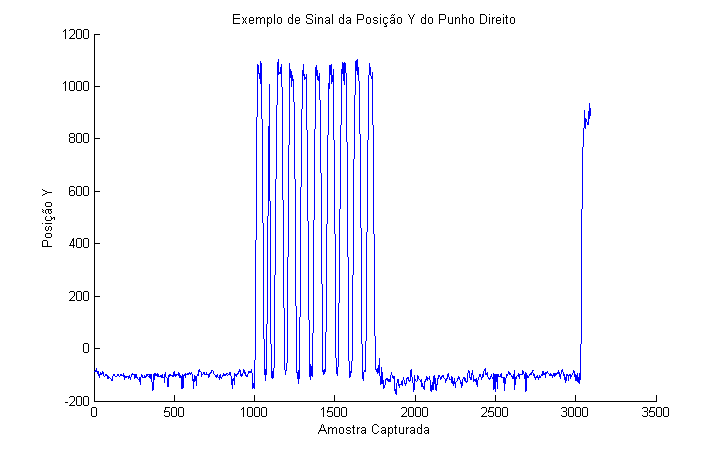
\includegraphics[width=1\textwidth]{./img/exsinalposicaoypunhodireito.png}
     \caption{Exemplo de Sinal Capturado da Articulação do Punho do Direito Usando MS-Kinnect na Posição Y}
     \label{img:exsinalposicaopunho}
\end{figure}

Em casos de análise de dados biomecânicos da amplitude do movimento é possível aplicar a técnica de detecção de picos e vales do sinal. Esta técnica consiste em usar um valor de referência $\delta$\ (\textit{delta}) para identificação dos picos e descartar valores menores que são considerados ruídos. O pico é o ponto mais alto entre os 2 pontos mais baixos que são considerados os vales do ciclo~\cite{peakdetect}. A técnica é aplicada no sinal da Figura~\ref{img:exsinalposicaopunho} com um $\delta$\ de 500 e teve como resultado os picos e os vales identificados como pode ser visto na Figura~\ref{img:expicosvales}.

\begin{figure}[!htb]
     \centering
     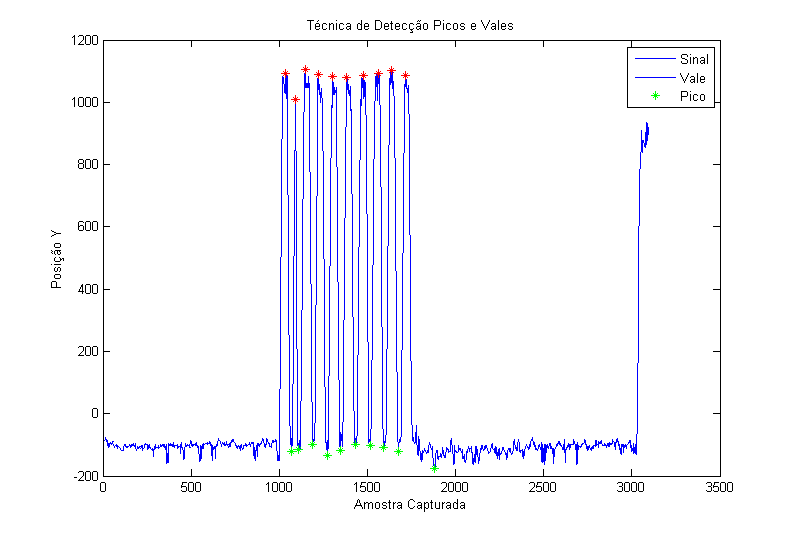
\includegraphics[width=1\textwidth]{./img/deteccaopicosvales.png}
     \caption{Exemplo da Aplicação da Técnica de Detecção de Picos e Vales no Sinal}
     \label{img:expicosvales}
\end{figure}


%\subsubsection{Redução de Ruídos no Sinal}
O processo de Identificação de Ciclos de Movimento é realizado em 3 etapas distintas:
\begin{itemize}
	\item Identificar ciclos de movimentos;
	\item calcular movimento angular realizado durante o ciclo de movimento;
	\item remover ciclos de movimentos incompletos.
\end{itemize}

Para identificar os ciclos de movimento de adução e abdução dos braços é necessário utilizar uma das articulações como referência. Neste movimento a articulação do punho (Figura~\ref{img:remocaoruidossinal}) é a que possui o sinal como maior amplitude entre as demais, por esse motivo esta é a escolhida para identificar os ciclos. Realiza-se a técnica de picos e vales no sinal do pinho para identificar o início e o fim do movimento de adução e abdução dos braços. Depois de identificado, onde começa e termina o movimento calcula-se o movimento angular através do produto escalar entre as articulações do punho, ombro e bacia(Seção~\ref{section:movimento_abducao}). Neste momento, o sinal irá conter ciclos de movimentos angulares, onde realiza-se uma nova eliminação de ruídos, ao extrair os ciclos de movimento identificados no sinal. Essa é a primeira etapa da filtragem dos dados, a qual seleciona o início e o fim dos ciclos de movimento. Depois desta etapa, realiza-se a extração de cada ciclo e identifica sua completude para que as características extraídas dos ciclos de movimento sejam semelhantes para cada indivíduo e torne possível a classificação dos dados.

\begin{figure}[!htb]
     \centering
     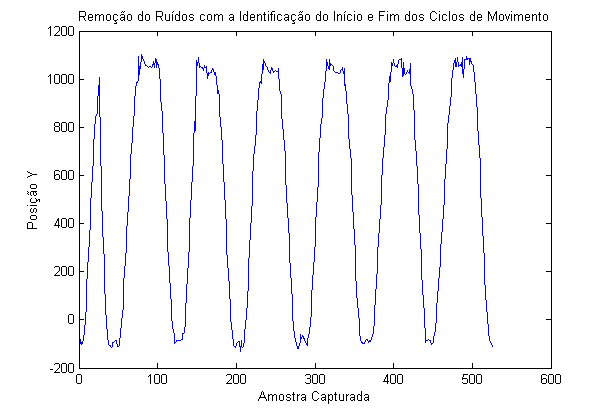
\includegraphics[width=1\textwidth]{./img/remocaoruidociclo.png}
     \caption{Remoção de Ruídos}
     \label{img:remocaoruidossinal}
\end{figure}


\subsection{Extração das Características do Movimento} \label{sec:extracao_caracteristcas}
As características do sinal a ser obtido é baseada na cinemática do movimento angular. Logo, é necessário um estudo da biomecânica do movimento humano nos ciclos de movimento ~\cite{hamill1999bases}. De posse do tempo de ocorrência de cada ciclo (\textit{Timestamp}) e das articulações do \textbf{punho}, \textbf{bacia} e \textbf{ombro} deve-se calcular o ângulo relativo do movimento de abdução e adução do braço através da aplicação do teorema do produto escalar (Equação~\ref{eq:produto_escalar}) que encontra o ângulo entre dois vetores dentro do intervalo de $0 \leq \theta \leq 180º$.

\subsubsection{Cálculo do Ângulo Relativo do Movimento de Abdução e Adução}\label{section:movimento_abducao}
O produto escalar é uma operação entre dois vetores cujo resultado é um escalar ~\cite{algebra90}. Então, o ângulo entre dois vetores é definido como ``o menor'' ângulo entre eles. Desta forma, este ângulo está dentro do intervalo de $0 \leq \theta \leq 180º $. O produto escalar é o ângulo de $ \theta$ formado entre os vetores $ v $ e $ w $ (Figura~\ref{img:produto_escalar}).


\begin{equation}
cos(\theta) = (v . w) /  (||v|| ||w||) 
\label{eq:produto_escalar}
\end{equation}


\begin{figure}[!htb]
     \centering
     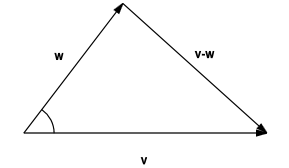
\includegraphics[width=0.5\textwidth]{./img/produtoescalar.png}
     \caption{Produto Escalar Entre 2 Vetores}
     \label{img:produto_escalar}
\end{figure}

No movimento de abdução e adução do braço (Figura \ref{fig:movabducaoaducao}), o ângulo relativo pode ser calculado com as Posições ($ x $\ ,  $ y $\ , $ z $\ ) das articulações (\textit{bacia}, \textit{ombro} e \textit{punho}). O código fonte em \textit{Matlab} ~\cite{matlab2011} realiza o cálculo do Produto Escalar dessas articulações e converte o valor escalar em °, para podermos extrair as características do movimento nessa unidade.

%O ângulo relativo podem ser calculados usando a Lei dos Cossenos. Essa lei é simplesmente um caso mais geral do Teorema de Pitágoras e descreve a relação entre os lados de um triângulo. Para nossos propósitos, o triângulo é constituído por dois segmentos (b e c) e uma linha (a) unindo a ponta distai de um segmento com a ponta proximal do outro ~\cite{hamill1999bases}.

\begin{figure}[!htb]
     \centering
     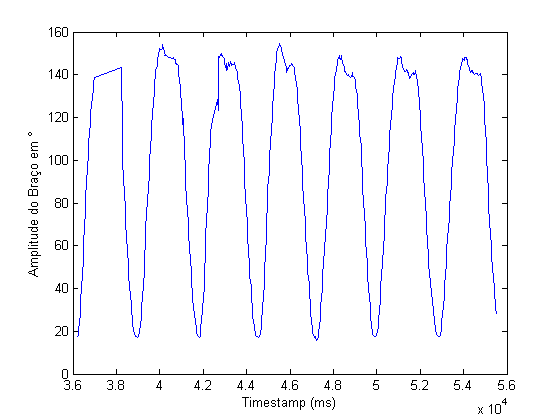
\includegraphics[width=1\textwidth]{./img/amplitude-braco.png}
     \caption{Amplitude do Movimento de Abdução e Adução}
     \label{img:amplitude_braco}
\end{figure}

Com o cálculo do produto escalar (Código Fonte~\ref{code:produto_escalar}) usando as três articulações, quantifica-se em °/ms o movimento de adução e abdução do braço em relação ao tempo criando o sinal desse movimento como na Figura~\ref{img:amplitude_braco}.

\lstset{language=Matlab}          % Set your language (you can change the language for each code-block optionally)
\begin{lstlisting}[frame=single, caption=Código do Ângulo Relativo por Produto Escalar, label=code:produto_escalar]  % Start your code-block
Bacia = [articulacaoBacia(PosicaoX), articulacaoBacia(PosicaoY), articulacaoBacia(Posicaoz)];
Ombro = [articulacaoOmbro(PosicaoX), articulacaoOmbro(PosicaoY), articulacaoOmbro(Posicaoz)];
Punho = [articulacaoPunho(PosicaoX), articulacaoPunho(PosicaoY), articulacaoPunho(Posicaoz)];

w = Bacia-Ombro;
v = Punho-Ombro;

CosTheta = dot(w,v)/(norm(w)*norm(v));
ThetaEmGraus = acos(CosTheta)*180/pi;
\end{lstlisting}

\subsubsection{Cálculo da Velocidade Angular do Movimento de Abdução e Adução}
O pico da amplitude do movimento irá conter a amplitude máxima desse movimento. O tempo gasto entre 1° vale até o pico em cada ciclo de movimento será o tempo gasto para a abdução do braço e o tempo gasto entre o pico e o 2° vale de cada ciclo será o tempo gasto para a adução do braço. Logo, com a amplitude máxima e o tempo gasto nesses movimentos podem ser calculadas as velocidades angulares de abdução e adução dos braços como na Figura~\ref{img:amplitude_braco_picos_vales}.
\begin{figure}[!htb]
     \centering
     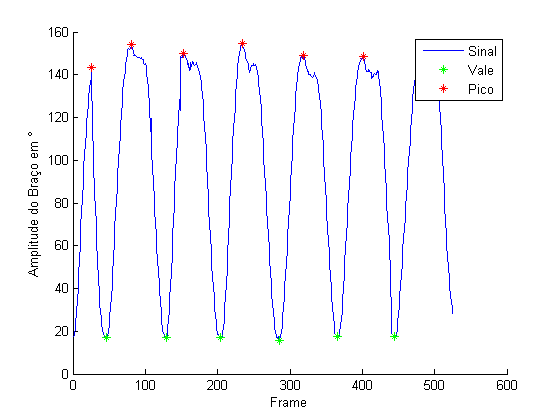
\includegraphics[width=1\textwidth]{./img/amplitude-braco-picos.png}
     \caption{Detecção de Picos e Vales da Amplitude do Movimento de Abdução e Adução do Braço}
     \label{img:amplitude_braco_picos_vales}
\end{figure}

\subsection{Filtragem de Dados}\label{section:filtro_dados}

A filtragem dos dados consiste na realização das seguintes etapas nos ciclos de movimento:
\begin{description}
	\item [Escalonar os ciclos]: O conjunto de dados deve possuir a distribuição de \textbf{M} amostras de vetores de dimensão \textbf{n}. Como os dados a serem analisados são sinais, deve-se então escalonar o sinal para uma dimensão \textbf{n} para poder realizar o cálculo matricial quadrático de (\textbf{M} x \textbf{n}).		
	\item [Normalizar os ciclos]: Em estatística o termo normalização possui diferentes significados ~\cite{statisticterms2006}. Neste trabalho, a normalização consiste no ajuste dos valores dos dados em torno do valor máximo. Ou seja o máximo valor obtido dos dados terá o valor 1 e os demais será o resultado pela divisão do valor máximo. A normalização se faz necessária para que a variação dos dados seja mantida além de facilitar a identificação de similaridades ~\cite{vicini2005}. 	
	\item [Calcular Vetor Médio dos Ciclos]: Para definir a completude de um ciclo de movimento deve-se inicialmente calcular a média entre todos os ciclos de movimento que é o vetor médio dos ciclos escalonados e normalizados (Figura ~\ref{img:ciclos_normalizado_escalonado}). O \textbf{vetor médio}, Equação (\ref{eq:vetormedio}), chamado de $\bar{X}$\ consiste na média aritmética de todos os ciclos de movimento ou seja calcula a centralização dos dados ~\cite{statisticshandbook2009}. 	
		\begin{equation}
			\bar{X}=\frac{\sum_{i=1}^{n}(Xi)}{(n)}
			\label{eq:vetormedio}
		\end{equation}
	\item [Calcular Variância de Cada Ciclo ao Vetor Médio]: A variância é uma medida de dispersão estatística, que indica o quão longe os estão de um valor esperado~\cite{statisticshandbook2009}. Neste caso o  valor esperado é o vetor médio dos ciclos ($\bar{X}$) e a variância, Equação (~\ref{eq:variancia}), irá nos informar o quão distante cada ciclo ($C$) está em relação a média.
		\begin{equation}
			var(C) = (C - \bar{X} )^2
			\label{eq:variancia}
		\end{equation}
		
		
	\item [Definir limiar para remoção de ciclos]: Essa etapa do processo de filtragem não é trivial, pois deve-se definir uma constante $ filtro $\ que será comparada à variância do ciclo, se esta for menor será aceita, caso contrário removida. Contudo,	balancear entre o limiar de dispersão do ciclo de movimento em relação a média é complexo, pois existe uma grande variabilidade de movimento. Logo, um limiar muito alto pode acarretar na remoção de uma grande quantidade de ciclos. Por outro lado, um limiar baixo pode colocar na base ciclos com ruídos e consequentemente impactar na classificação dos dados.	
	\lstset{language=Matlab}
	\begin{lstlisting}[frame=single, caption=Filtro dos Ciclos]  % Start your code-block
		
    filtro = 1;
    vetorMedio = mean(ciclos);
    varianciaCiclo = sum(ciclo - (vetorMedio).^2);
    remocao = varianciaCiclo>filtro;
	\end{lstlisting}
	
	\begin{figure}
     \centering
     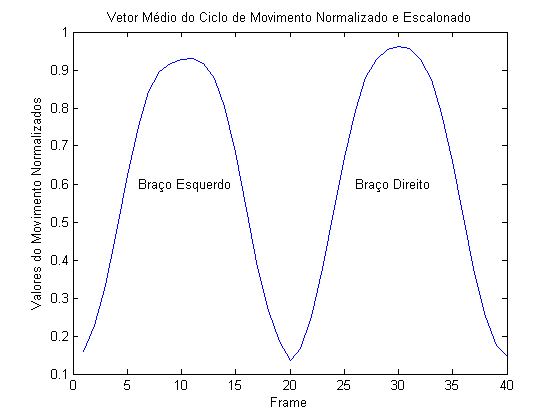
\includegraphics[width=1\textwidth]{./img/vetormedionormalozadoescalonado.png}
     \caption{Ciclos de Movimento Normalizados e Escalonados}
		 \label{img:ciclos_normalizado_escalonado}
	\end{figure}
\end{description}


%\lstset{language=Matlab}
%\begin{lstlisting}
	%normalizarCiclos(ciclos);
	%escalonarCiclos(ciclos, CONSTANTE_ESCALONAMENTO);
	%vetormedio = mean(ciclos);
	%
	%
%\end{lstlisting}

%%Média

Como exemplo, temos um ciclo de movimento filtrado (Figura~\ref{img:ciclo_filtrado}) (\textit{valor do filtro = 1}) e o (\textit{valor da variância = 2,3078}).

\begin{figure}[!htb]
     \centering
     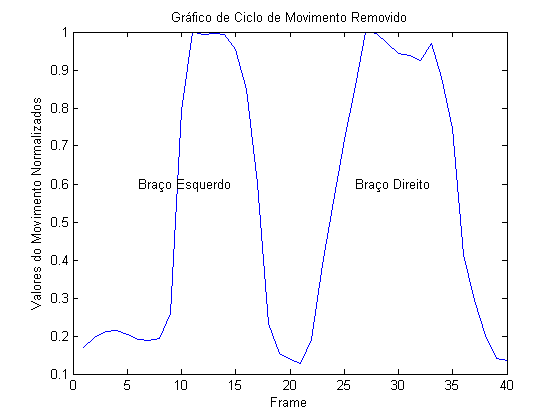
\includegraphics[width=1\textwidth]{./img/ciclomovimentoremovido.png}
     \caption{Ciclo de Movimento Removido}
		 \label{img:ciclo_filtrado}
\end{figure}





%Para filtrar os dados baseado na distância dos mesmos em relação a média, devemos realizar uma subtração de cada ciclo normalizado e escalonado (\textit{cne}) pelo vetor médio (\textit{vetormedio}). Em seguida deve ser realizada uma exponenciação por dois de modo que teremos um valor positivo que possa quantificar essa discrepância Eq.~\ref{eq:filtro}. O limiar para remoção dos dados irá depender do resultado dessa quantificação como explicado anteriormente.




%\begin{equation}
%filtro = (\sum (\left[ cne\right] - \left[\bar{X} \right])^2) > limiar
%\label{eq:filtro}
%\end{equation}


%\subsubsection{Rotular ciclos de movimento}\label{section:rotular_ciclos}

%\subsubsection{Normalizar os ciclos}\label{section:normalizar_ciclos}


%\subsubsection{Escalonar os ciclos}\label{section:escalonar_ciclos}

%\subsubsection{Definir limiar}\label{section:escalonar_ciclos}

\section{Classificação de Dados por Máquina de Aprendizagem}\label{section:class_dados}
O objetivo de todo esse processo de identificação de ciclos, extração de características e filtragem é justamente facilitar a separação dos dados por máquinas de aprendizagem. O resultado desta etapa resulta num conjunto de ciclos de movimento processados onde podemos visualizar na Figura ~\ref{fig:ciclos_movimento_processados_filtrados}. Percebam na mesma figura a grande variabilidade de movimento existente entre os indivíduos diagnosticados com a Doença de Parkinson e Indivíduos sem o diagnóstico da doença. A normalização dos ciclos, ficou sendo o resultado do cálculo do Produto Escalar que nos retorna valores entre $ 0° $\ a $ 180° $\ do movimento de abdução e adução. O escalonamento de cada ciclo de movimento ficou com 20 \textit{frames} como temos o movimento do braço esquerdo e depois o do direito temos um total de 40 \textit{frames} por ciclo. O motivo que decidimos juntar os ciclos do braço esquerdo e direito lado a lado foi justamente para facilitar a identificação da assimetria do movimento 
existente nos estágios iniciais da ~\ac{dp}.

\begin{figure}[!htbp]
 \centering
 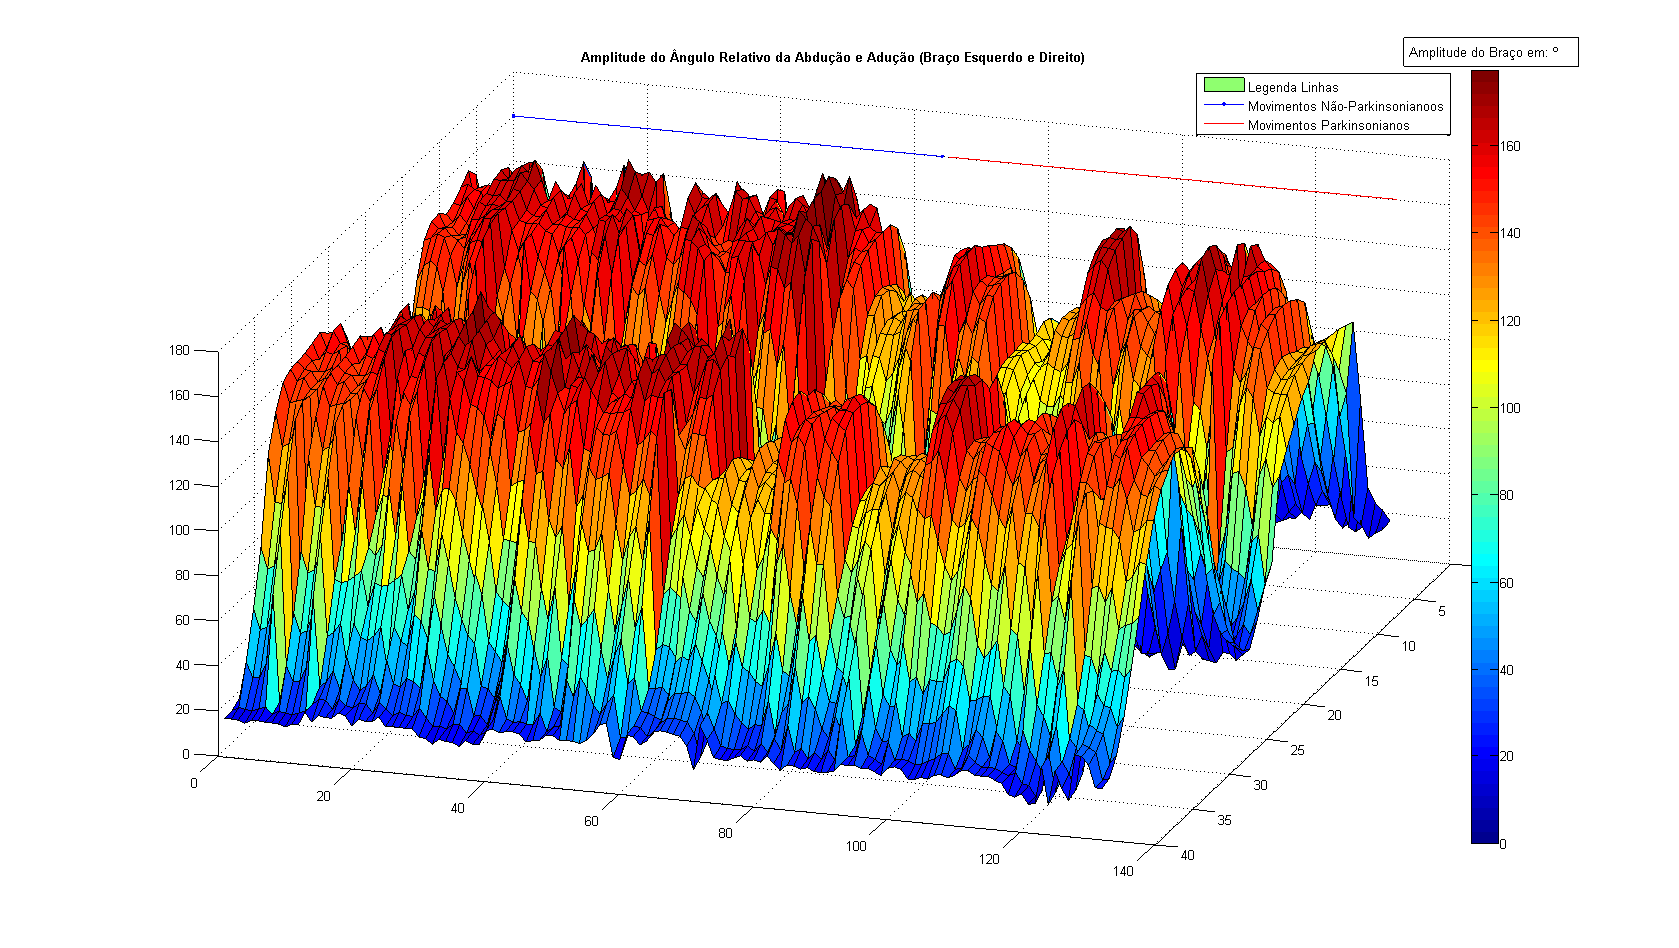
\includegraphics[scale=0.38]{./img/ciclosmovimentokinnect.png}
 \caption{Ciclos de Movimento Abdução e Abdução Usados na Classificação}
 \label{fig:ciclos_movimento_processados_filtrados}
\end{figure}


O vetor de características é composto dos ciclos de movimento e das características extraídas de cada ciclo conforme explicado na Seção~\ref{sec:extracao_caracteristcas}. Ou seja, terá além do ciclo de movimento, os valores da velocidade angular de abdução e adução do braço esquerdo e direito. De posse desse vetor de características e do rótulo sobre a classe do ciclo de movimento (indivíduo diagnosticado com a ~\ac{dp} e indivíduo sem o diagnóstico estabelecido) esses dados serão repassados juntamente como entrada-saída para o classificador de dados que irá dividir entre grupos de treinamento e teste para realizar sua classificação.

Utiliza-se então o classificador de dados como um identificador de possíveis usuários com problemas motores. Logo, o classificador irá auxiliar o profissional de saúde no acompanhamento de seus pacientes. Pois, supondo um profissional de saúde o qual possui um grande número de pacientes que são usuários da abordagem \textit{GAHME} para monitorar seus dados. Um classificador de dados por máquina de aprendizagem seria utilizado para identificar sintomas motores nos indivíduos. Caso um indivíduo fosse identificado com um sintoma pelo classificador, o profissional de saúde poderia visualizar os dados quantificados para realizar a sua tomada de decisão. Logo a responsabilidade da tomada de decisão é do profissional, por esse motivo é que a abordagem \textit{GAHME} serve como apoio ao diagnóstico e acompanhamento dos sintomas motores.


\section{Visualização dos Dados}
O acompanhamento de sintomas motores se faz necessário, principalmente para doenças crônicas de impacto motor e que tenham melhoria nos sintomas. Pois desta forma, auxilia-se o médico no acompanhamento motor e consequentemente permite tratar o paciente de acordo com a resposta ao tratamento.

Como exemplo da abordagem , o profissional de saúde poderia visualizar as características do movimento que serviram como dados de entrada para a máquina de aprendizagem. Nesse caso, podemos ver duas tabelas em que é possível identificar as diferenças motoras de uma pessoa diagnostica com a ~\ac{dp} (Tabela \label{table:extracao_caracterisca_parkinsoniano}) e um indivíduo sem o diagnóstico da doença (Tabela ~\ref{table:extracao-caracteristica}).

\begin{table}[h]
\begin{tabular}{|r|r|r|r|r|r|}
\hline
\multicolumn{4}{|l}{Velocidades º/S}                                                                                                                                                                                                                                                                                         & \multicolumn{2}{|l|}{Amplitudes}     \\ \hline
\multicolumn{1}{|l}{\textbf{\begin{tabular}[c]{@{}c@{}}Abdução\\ Esquerda\end{tabular}}} & \multicolumn{1}{|l|}{\textbf{\begin{tabular}[c]{@{}c@{}}Abdução\\ Direita\end{tabular}}} & \textbf{\begin{tabular}[c]{@{}c@{}}Adução\\ Esquerda\end{tabular}} & \textbf{\begin{tabular}[c]{@{}c@{}}Adução\\ Direita\end{tabular}} & \textbf{Esquerda} & \textbf{Direita} \\ \hline
78,95                                                                                    & 77,82                                                                                    & 83,06                                                              & 106,42                                                            & 130,00            & 124,72           \\ \hline
79,94                                                                                    & 34,68                                                                                    & 104,69                                                             & 39,98                                                             & 131,50            & 132,44           \\ \hline
81,05                                                                                    & 47,05                                                                                    & 107.38                                                             & 56,52                                                             & 132,22            & 123,66           \\ \hline
74,73                                                                                    & 47,09                                                                                    & 109,05                                                             & 47,75                                                             & 132,33            & 122,20           \\ \hline
72,01                                                                                    & 56,02                                                                                    & 102,36                                                             & 76,00                                                             & 131,40            & 119.75      \\ \hline
\end{tabular}
\caption{Extração das Características de Indivíduo Com Diagnóstico da ~\ac{dp}}
\label{table:extracao-caracteristica}
\end{table}

\begin{table}[h]
\begin{tabular}{|r|r|r|r|r|r|}
\hline
\multicolumn{4}{|l}{Velocidades º/S}                                                                                                                                                                                                                                                                                         & \multicolumn{2}{|l|}{Amplitudes}       \\ \hline
\multicolumn{1}{|l}{\textbf{\begin{tabular}[c]{@{}c@{}}Abdução\\ Esquerda\end{tabular}}} & \multicolumn{1}{|l|}{\textbf{\begin{tabular}[c]{@{}c@{}}Abdução\\ Direita\end{tabular}}} & \textbf{\begin{tabular}[c]{@{}c@{}}Adução\\ Esquerda\end{tabular}} & \textbf{\begin{tabular}[c]{@{}c@{}}Adução\\ Direita\end{tabular}} & \textbf{Esquerda} & \textbf{Amplitude} \\ \hline
129,35                                                                                   & 61,59                                                                                    & 78,74                                                              & 176,30                                                            & 159,39            & 143,50             \\ \hline
115,67                                                                                   & 118,15                                                                                   & 71,72                                                              & 79.46                                                             & 156,37            & 153,97             \\ \hline
120.96                                                                                   & 135,27                                                                                   & 66,70                                                              & 78,17                                                             & 154,30            & 149,91             \\ \hline
125.96                                                                                   & 137,43                                                                                   & 64,75                                                              & 81,57                                                             & 153,18            & 154,58             \\ \hline
139.99                                                                                   & 117,60                                                                                   & 69,96                                                              & 84,08                                                             & 151,68            & 148,90             \\ \hline
120,51                                                                                   & 111,92                                                                                   & 75,85                                                              & 75,18                                                             & 152,58            & 148,35             \\ \hline
\end{tabular}
\caption{Extração das Características de Indivíduo Sem Diagnóstico da ~\ac{dp}}
\label{table:extracao_caracterisca_saudavel}
\end{table}

Como pode ser visto nesses dados a amplitude de de um indivíduo diagnosticado com a~\ac{dp} esta bem menor do que um indivíduo sem o diagnóstico estabelecido. Um valor importante também pode ser identificado na velocidade de adução esquerda do indivíduo com ~\ac{dp} possui uma velocidade muito maior do que o indivíduo sem o diagnóstico. Possivelmente porque um paciente da ~\ac{dp} perde um pouco o controle sobre o membro fazendo-o descer abruptamente ~\cite{protpar010}. Desta maneira pretende-se com a abordagem, auxiliar o profissional de saúde com o fornecimento dessa informação para que este venha efetuar o acompanhamento e perceba a evolução do quadro clínico do paciente.

%O produto escalar é uma operação entre dois vetores cujo resultado é um escalar e pode ser descrito na forma:
%$ u.v = |u| |v| cos(\theta) $\ onde $ \theta $\ é o ângulo formado entre $ u $\ e $ v $\ dentro do intervalo de $0 \leq \theta \leq 180º $\.

%Se
%\begin{math}
%v.w = \left \| v \right \|\left \| w \right \|\cos \theta
%\end{math}
%, onde $ \theta $\ é o ângulo entre esses vetores. Então o \textbf{ângulo} entre dois vetores é definido como o menor ângulo entre eles.
%
%Portanto, o ângulo dentro do intervalo de $0 \leq \theta \leq 180º $\ será o resultado do produto interno
%\newline
%\begin{math} \cos \theta = (v.w)/(\left \| v \right \| \left \| w \right \|)\end{math} .

%\subsubsection{Pontos Utilizados no \textit{Ms-Kinnect} Para o Cálculo do Produto Escalar}
%A descrição da posição de um segmento ou movimento articular é tipicamente expressa com relação a uma posição inicial designada. A posição anatômica é uma referência padronizada usada por muitos anos por anatomistas, biomecânicos e médicos ~\cite{hamill1999bases}.



%\begin{figure}
 %\centering
 %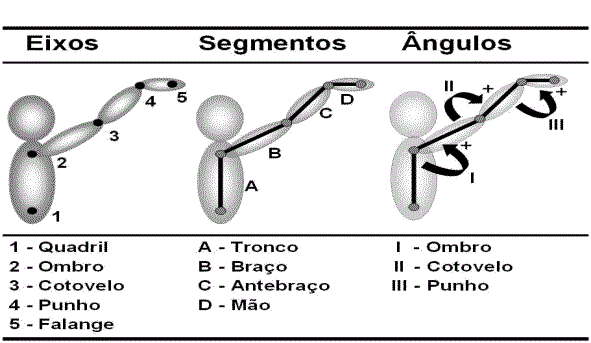
\includegraphics[scale=0.5]{./img/eixossegmentos.png}
 %% matrixargseg.png: 296x162 pixel, 100dpi, 7.52x4.11 cm, bb=0 0 213 117
 %%\caption{Estágio desenvolvimento de jogos ~\cite{fullerton2008game}}
%\caption{Eixos Segmentos e Ângulos da Biomecânica}
%%  \caption{Estágio desenvolvimento de jogos}
 %\label{fig:eixossegmentos}
%\end{figure}

%\chapter{Metodologia de Pesquisa}
A metodologia de pesquisa utilizada nesse trabalho, possui aspectos qualitativos que permitem identificar a importância deste trabalho junto à comunidade de especialistas da área de saúde e também possui aspectos quantitativos que demonstram que a abordagem utilizada consegue diferenciar indivíduos com portadores da doença de parkinson perante indivíduos que não desenvolveram a doença por intermédio de sensores de movimento e de força. O desfecho da pesquisa se fará com o resultado tanto da pesquisa qualitativa quanto da pesquisa quantitativa.

\section{Desenho da Pesquisa} \label{sec:desenho_pesquisa}
Para uma melhor compreensão da pesquisa temos o Desenho da Pesquisa a ser realizada na Figura \ref{figure:desenho_pesquisa} e a descrição de cada um dos passos.


A Problemática desse trabalho, já foi descrita na Seção \ref{section:problematica}. A revisão da literatura irá consistir de uma descrição sobre a doença estudada como estudo de caso (Doença de Parkinson) que está descrito no Capítulo \ref{section:doenca_parkinson}, bem como da possibilidade de integrar o monitoramento da doença de Parkinson por intermédio de jogos eletrônicos. 


\begin{figure}[!htbp]
    \centering
    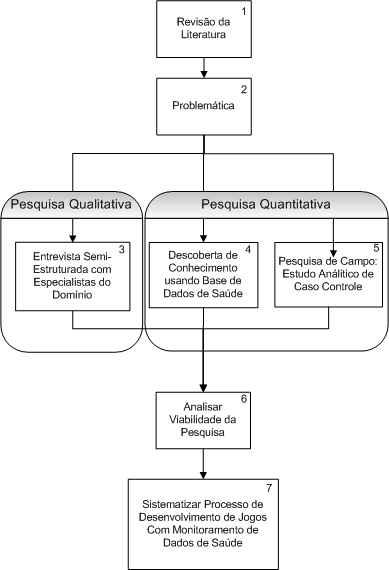
\includegraphics[width=.7\textwidth]{./img/metodologia-pesquisa.png}
    \caption{Desenho da Pesquisa}
    \label{figure:desenho_pesquisa}
\end{figure}

\section{Pesquisa Qualitativa}
Essa pesquisa tem como objetivo identificar a importância de realizar o monitoramento de dados de saúde por intermédio jogos eletrônicos. Em um primeiro momento, serão verificados junto a comunidade médica a relevância desse trabalho e se este poderia auxiliar no monitoramento dos sintomas parkinsonianos. 

Os pesquisadores que adotam a abordagem da pesquisa qualitativa a fazem por sua flexibilidade, sem regras rígidas, aplicáveis a uma ampla gama de casos e formalizações pré-definidas, possibilitando a construção de modelos abrangentes \cite{Gom00}. 
Nesse estudo a pesquisa qualitativa está orientada a um estudo de caso, partindo da análise das expressões e comportamento das pessoas. Na busca por entender os fenômenos sociais complexos, o estudo de caso permite uma investigação significativa nas mudanças desses processos\cite{Yin05}.

Por se tratar de um estudo empírico, utilizamos a pesquisa qualitativa por envolver uma grande variedade de técnicas para levantamento de informações (entrevistas, observações, histórico, interações, artefatos e ferramentas utilizadas) \cite{FLI04}.

%Partindo da problemática da pesquisa \ref{section:problematica}, essa pesquisa busca identificar por intermédio de uma técnica de pesquisa qualitativa de Entrevista Semi-Estruturada junto a profissionais de saúde a importância do monitoramento dos dados de saúde

%esse texto abaixo está repetido na problemática



%Nessa seção iremos descrever a metodologia de pesquisa adotada no
%estudo. Na seção 1 apresenta-se o desenho da pesquisa com suas
%respectivas etapas. Na seção 2 apresenta os aspectos metodológicos
%do estudo. Na seção 3 apresenta-se a operacionalização das
%variáveis. Por último, na seção 4, é apresentada a base metodológica
%do estudo.
\subsection{Entrevista Semi-Estruturada Com Especialistas do Domínio (3)}\label{section:entrevista_semi-estruturada}

O objetivo deste procedimento foi entender como é feito o acompanhamento dos sintomas da doença de parkinson juntamente aos profissionais de saúde (neurologistas que prescrevem a dosagem medicamentosa e fisioterapeutas que fazem o acompanhamento motor do paciente ao longo de seu tratamento). Os mesmos foram indagados se poderia haver melhora na tomada de decisão caso eles pudessem acompanhar o surgimento dos sintomas em diferentes momentos do dia por intermédio de um monitoramento frequente dos sintomas. Procurou-se encontrar dentro do contexto de estudo, a importância do monitoramento de dados de saúde e os benefícios trazidos por este.

\subsubsection{Perfil dos participantes}

O público alvo da pesquisa são profissionais de saúde especialistas em doenças neurológicas e acompanhamento motor que realizam acompanhamento de pacientes com a doença de parkinson. Devido a sua formação, esses profissionais são aptos a fornecer subsídios para o desenvolvimento da solução proposta neste trabalho.

Logo no início da entrevistas devem ser obtidas informações sobre a formação acadêmica, tempo de experiência e área de atuação.

%, de modo auxiliar na visualização do contexto da pesquisa uma tabela foi elaborada com o perfil de cada participante. %COLOCAR REFERENCIA DE TABELA%


As entrevistas foram realizadas de maneira presencial, onde primeiramente fez-se perguntas não estruturadas e havendo uma maior estruturação no decorrer da entrevista com a preocupação de que seja evitada a referência do entrevistador seja sobre os pontos de vista do entrevistado conforme prega o método científico \cite{FLI04}. Durante a pesquisa foi utilizado recursos de gravação, de modo a facilitar a transcrição dos dados coletados. %[Uma tabela resumindo as principais características das pessoas]

\subsubsection{Entrevista com Profissionais de Saúde Especialistas em Neurologia} 
Essa etapa da pesquisa foi baseada num conjunto de questões/guia vide Apêndice \ref{apendice:entrevista-semi-estruturada}, onde nem todas as perguntas elaboradas foram utilizadas.

Para a construção do questionário foi realizada uma análise sobre a doença de parkinson e sintomas que pudessem ser monitorados usando sensores, para a construção do questionário foram utilizadas diretrizes médicas da Doença de Parkinson ~\cite{protpar010,national2006parkinson} e da tabela UPDRS ~\cite{updrs87} usada para avaliação do progresso da doença ~\cite{updrs87}.

A entrevista semi-estruturada realizada teve um total de 15 perguntas agrupadas em 3 seções, com os seguintes temas: sintomas da doença de parkinson, monitoramento da saúde motora e os benefícios advindos do monitoramento. Devido as diferenças existentes na abordagem utilizada por cada profissional o entrevistador poderá selecionar as questões de acordo com suas características.

%\section{Analisar Viabilidade da Pesquisa (6)} A análise de resultados servirá de base para o desenvolvimento do processo proposto. Dando o suporte necessário para a seleção de um conjunto de ferramentas a serem incorporadas na execução do processo. 
%A análise do resultado está descrita no \chapref{chapter:analise_resultados}.

\subsection{Análise da Entrevista Semi-Estruturada}

Como o método de pesquisa da entrevista Semi-Estruturada é qualitativo. Será realizada uma pesquisa qualitativa assistida por computador utilizando-se o \textit{software} QDA Miner \cite{qda13}. Este \textit{software} permite a análise qualitativa das informações obtidas em modo texto. Software dessa natureza auxiliam o pesquisador na organização dos registros da pesquisa e das interpretações dos mesmos. A escolha dessa ferramenta é justificada pela dificuldade de classificar e analisar os dados obtidos. Nessa análise somente foram levadas em consideração as atividades referentes ao acompanhamento dos sintomas motores em pacientes de parkinson e como um possível cenário que permitisse o monitoramento desses sintomas por intermédio de jogos eletrônicos poderia auxiliar os pacientes e também os profissionais de saúde.

\subsubsection{Instrumento de Análise dos Dados da Pesquisa Qualitativa} \label{section:analise_dados} 

A interpretação de dados é o cerne da pesquisa qualitativa. Tem como função desenvolver a teoria, servindo ao mesmo tempo de base para a decisão sobre quais dados adicionais devem ser coletados \cite{FLI04}.

É importante que seja realizada a codificação seletiva, para que seja elaborada a categorização essencial sobre todas as categorias envolvidas \cite{FLI04}. O pesquisador precisa decidir quais os fenômenos salientes e ponderá-los de forma a ter como resultado uma categoria central juntamente com as categorias a ela relacionadas.

O procedimento da interpretação dos dados, assim como a integração de material adicional, é encerrado quando atinge a "saturação teórica", quando o avanço da codificação não atinge mais novos conhecimentos \cite{FLI04}.

Para análise dos textos provenientes da pesquisa (transcrição da entrevista com os Neurologistas e Fisioterapeutas especialistas em Neurologia) foi utilizada a codificação seletiva através de criação de categorias a \emph{posteriori}. As categorias foram criadas e organizadas de acordo com o conteúdo de cada texto. As respostas de cada participante foram analisadas e a partir da identificação das categorias, incluídas na árvore de categorias do QDA Miner \cite{qda13}, que possui a transcrição de cada questionário e interação ocorrida. Admitindo-se que uma classificação, para ser adequada não pode ser feita arbitrariamente, a categorização da árvore será criada e reformulada várias vezes, durante o processo de análise de acordo com \cite{FLI04}.

Por fim, com base na análise do texto, foram verificados dificuldades, necessidade, importância e viabilidade da pesquisa do ponto de vista dos profissionais de saúde.
 
\section{Descoberta de Conhecimento usando Base de Dados de Saúde}
Para esse estudo, foram utilizados dados do \textit{PhysioBank} ~\cite{physionet}. O \textit{PhysioBank} armazena sinais fisiológicos e dados relacionados a comunidade de pesquisa biomédica, incluindo sinais vitais, motores de indivíduos saudáveis e de pacientes com uma variedade de sintomas como distúrbios neurológicos ou envelhecimento. 

\subsection{Materiais}
Para a presente pesquisa, foi utilizada a base de dados "\textit{Parkinson´s Disease Database}" ~\cite{physionet} a qual contém as medidas da marcha de 93 pacientes com doença de Parkinson idiopática (idade média: 66,3 anos, 63$\%$ homens) e 73 controles saudáveis ​​(com idade média de 66,3 anos, 55$\%$ homens). Esse banco de dados inclui os registros da \ac{fvrs} de indivíduos enquanto eles caminhavam normalmente em seu próprio ritmo por aproximadamente 2 minutos em um terreno plano. Debaixo de cada pé foram postos oito sensores (Figura \ref{fig:posicaosensores}) (\texit{Ultraflex Computer Dyno Graphy} da \texit{Infotronic Inc.} ~\cite{dyno}) (Figura \ref{fig:dynography}) que captavam a força desempenhada pelo corpo sobre o solo, essa força foi medida em Newtons sobre o tempo. 

\begin{figure}[!htbp]
 \centering
 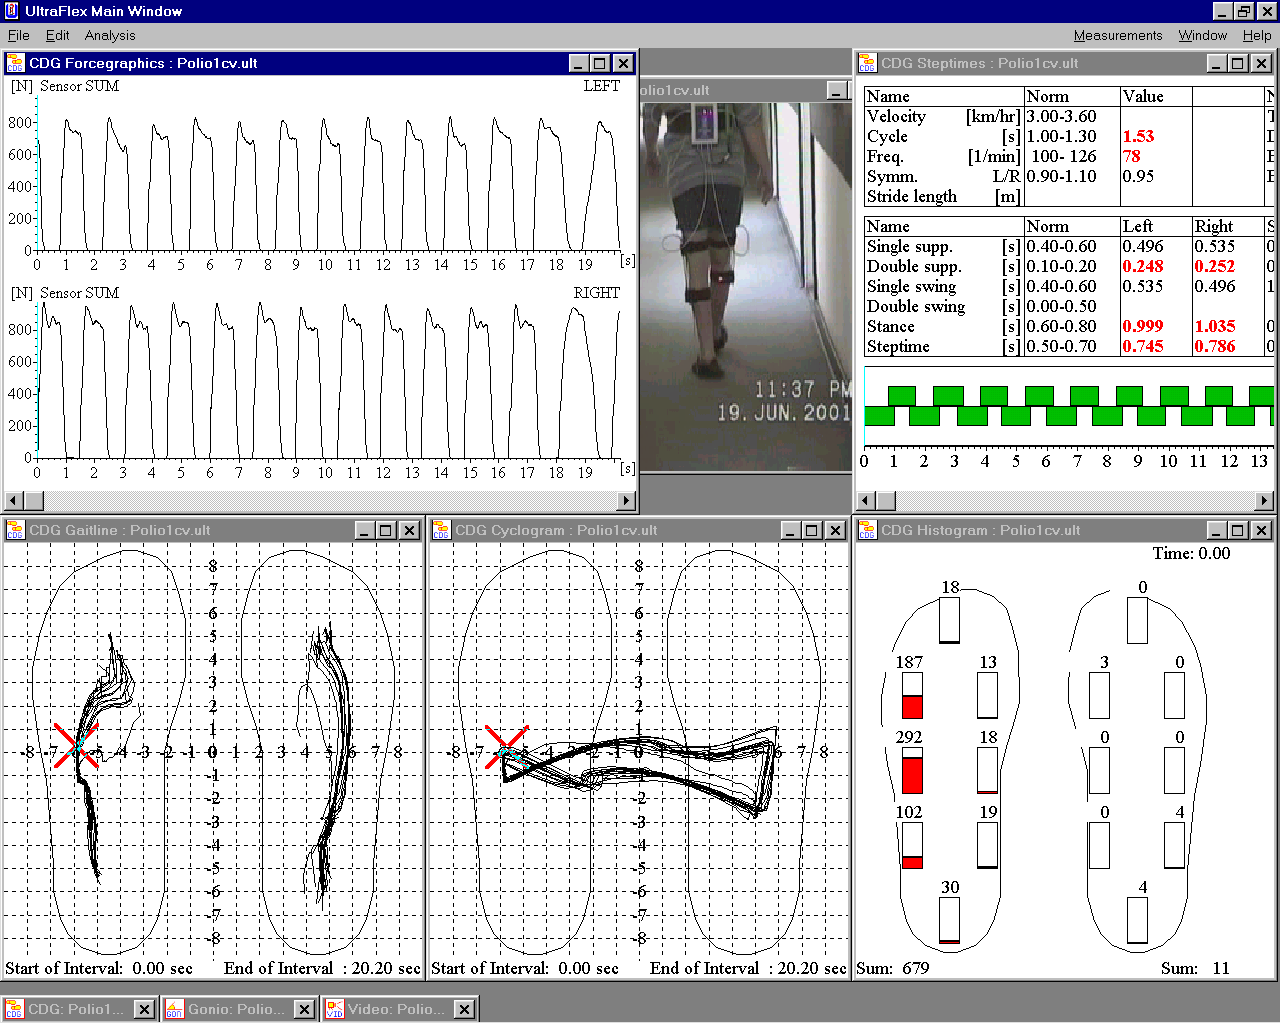
\includegraphics[scale=0.4]{./img/ultraflexdinografia.png}
 % matrixargseg.png: 296x162 pixel, 100dpi, 7.52x4.11 cm, bb=0 0 213 117
 %\caption{Estágio desenvolvimento de jogos ~\cite{fullerton2008game}}
\caption{\texit{Ultraflex Computer Dyno Graphy}}
%  \caption{Estágio desenvolvimento de jogos}
 \label{fig:dynography}
\end{figure}

\begin{figure}[!htbp]
 \centering
 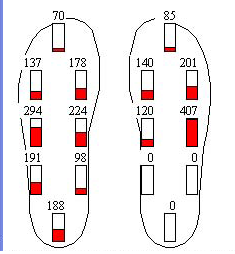
\includegraphics[scale=0.7]{./img/ultraflexposition.png}
 % matrixargseg.png: 296x162 pixel, 100dpi, 7.52x4.11 cm, bb=0 0 213 117
 %\caption{Estágio desenvolvimento de jogos ~\cite{fullerton2008game}}
\caption{Posição dos Sensores}
%  \caption{Estágio desenvolvimento de jogos}
 \label{fig:posicaosensores}
\end{figure}

A saída de cada um destes 16 sensores foi armazenada e gravada em 100 amostras por segundo, nesses registos estão inclusos dois sinais que refletem a soma da medição dos oito sensores para cada um dos pés sendo denominada de \ac{fvrs} do pé Esquerdo e Direito respectivamente ~\cite{gaitusingsensorsreview2012}, para esse trabalho foi utilizado o resultado desta soma para realizar a análise de movimento.

\subsection{Método}\label{section:metodo_parkinson_database}
Para a análise desses dados, foi utilizado um método de reconhecimento de faces bem estabelecido chamado de \textit{eigenfaces}~\cite{eigenfaces91}. Nós criamos o  método \textit{eigengaits} ~\cite{medeiros2013} para identificar características e padrões que pudesse classificar pessoas diagnosticadas com a doença de parkinson ante indivíduos sem o diagnóstico estabelecido.

A análise dos dados da \textit{Parkinson Disease Database} ~\cite{physionet}, incluiu 50 pacientes de Parkinson e 50 indivíduos que não possuíam desenvolvido a doença (segundo as informações fornecidas pela própria base de dados). Foram calculados, normalizados e escalonados em 80 \textit{frames} um total de 120 ciclos de marcha (Seção \ref{section:analise_marcha}) que foram usados para efetuar a técnica de aplicar a técnica \textit{eigengaits} ~\cite{medeiros2013} que é uma adaptação da Análise dos Componentes Principais que será explicada na Seção \ref{section:analise_marcha_pca}. 


\section{Estudo analítico de caso-controle}\label{section:estudo_caso_controle}
Esta etapa da pesquisa foi pautada pelo protocolo de pesquisa submetido à avaliação do Comitê de Ética da UFCG, somente após a aprovação deste (\textbf{CAAE: 14408213.9.1001.5182}) é que os dados foram coletados. 
Os resultados que se desejou alcançar com a pesquisa foi o descobrimento de mecanismos para a identificação e classificação de pessoas saudáveis ante os portadores de doença de parkinson. Durante a pesquisa também analisou-se o sensor de movimento MS-Kinnect ~\cite{kinnect2013} para avaliar a possibilidades de aquisição de dados de saúde baseada na Cinemática Linear do Movimento Humano.  

Através dos resultados obtidos pretendemos avaliar e classificar a normalidade e dificuldade na execução de movimentos como levantar um braço por exemplo.

A coleta de dados foi realizada nas seguintes instituições (Hospital Universitário UFAL, Fundação Pestalozzi - Maceió) sob a tutela da Profa. e Neurologista Dra. Cícera Pontes; e na Clínica de Fisioterapia do CESMAC sob a tutela do Prof. de Fisioterapia Jean Charles Santos, ambas realizadas em local reservado e de forma individual com a anuência do sujeito pesquisado através da assinatura do Termo de Consentimento.

\subsection{Amostra}
A técnica de amostragem utilizada para seleção, foi por conveniência onde foi composta por indivíduos 15 indivíduos diagnosticados com ~\ac{dp} e 12 indivíduos sem o diagnóstico como grupo de controle. 

\subsection{Recrutamento dos Sujeitos e Aquisição do Consentimento Livre e Esclarecido}
A forma de recrutamento deste protocolo será Circunscrita por intermédio de um profissional de saúde. O profissional deverá conhecer a história clínica do paciente e obterá a permissão do mesmo para que a equipe de pesquisa possa entrar em contato.
A equipe de pesquisa deverá explicitar os riscos e benefícios da participação da pesquisa buscando a espontaneidade da decisão e depois fornecer o Termo De Consentimento Livre E Esclarecido.

\subsection{Critérios de Inclusão}
Os indivíduos do grupo diagnosticados a \ac{dp} precisam estar no estágio 3 segundo a UPDRS ~\cite{updrs87}, sem distinção de sexo ou raça, que estejam dentro das facilidades da Clínica onde a coleta esteja sendo realizada e que aceitem participar do estudo.
Os indivíduos sem o diagnóstico da \ac{dp}, precisam informar que não possuem o diagnóstico da doença e aceitem a participar do estudo como grupo controle.

\subsection{Critérios de Exclusão}
Pessoas com sintomas motores e que tenham problemas em equilíbrio, questionamento de dores ao executar os procedimentos além daqueles que por qualquer motivo se negaram a participar do estudo.

\subsection{Materiais}
Para a presente pesquisa foi coletados movimentos de abdução e adução dos braços, que pudessem ser incorporados em um jogo eletrônico. Foi utilizado um jogo com o arcabouço de software de captura de dados desenvolvido por um aluno de Mestrado da Universidade Federal de Campina Grande ~\cite{antonio2013} juntamente com um aluno de iniciação científica do IFAL. Os dados foram coletados e depois processados e classificados com a abordagem apresentada nessa Proposta de Tese. 

Durante a execução desta coleta, houve uma preocupação com a integridade física dos participantes, muitos possuíam receio de quedas, logo os movimentos utilizados no jogo foram apenas de adução e abdução dos braços ~\cite{mcginnis2013biomechanics}, trazendo segurança aos participantes do grupo de indivíduos com \ac{dp}. 

\subsubsection{Infra-Estrutura}
A pesquisa será realizada na Clínica em que o paciente está em tratamento, onde são realizados tratamentos fisioterápicos ou consultas. O espaço físico forneceu condições favoráveis e adequadas para aplicação dos jogos. Para a realização da pesquisa foram utilizados:

\begin{itemize}
	\item Jogo (\textit{Catch the Spheres} rodando em notebook com Sistema Operacional Windows 7.0 e Unity 3d 3.0;
	\item Projetor (Epson Lcd Powerlite X14 3000l Hdmi) para projetar o jogo na parede e facilitar a visualização;
	\item Sensor de movimento Ms-Kinnect ~\cite{kinnect2013}.
\end{itemize}

\subsection{Métodos}
Essa pesquisa também fez uma análise de um sensor de movimento utilizados em jogos eletrônicos e avaliou a possibilidades de aquisição de dados de saúde baseada na Cinemática Angular do Movimento Humano ~\cite{hamill1999bases}.  Através dos resultados obtidos pretendemos avaliar e classificar a normalidade e dificuldade na execução de movimentos como abdução e adução dos braços.

A coleta de dados foi realizada no próprio espaço de tratamento do indivíduo em local reservado e de forma individual e permitindo sua participação por meio do Termo de Consentimento. Devido as restrições de tempo (1 minuto e 30 segundos) e a execução de um mesmo movimento por todos os participantes, foi solicitados que cada voluntário da pesquisa executassem os seguintes procedimentos:
\begin{enumerate}
	\item O voluntário se posiciona a uma distância de 2 metros do sensor de movimento, de modo a conseguir capturar toda a extensão superior do braço durante o movimento de abdução; 	
	\item O voluntário inicia o jogo \textit{Catch the Spheres} usando a mão esquerda conforme a interface da aplicação;
	\item O voluntário levanta 10 vezes o braço esquerdo e depois o braço direito o mais alto e mais rápido que consegue, de modo a permitir que fosse capturados a amplitude de movimento e a velocidade angular do mesmo. 
	\item O voluntário fecha a aplicação e esta realiza o armazenamento dos dados.
\end{enumerate}

\begin{figure}[!htbp]
 \centering
 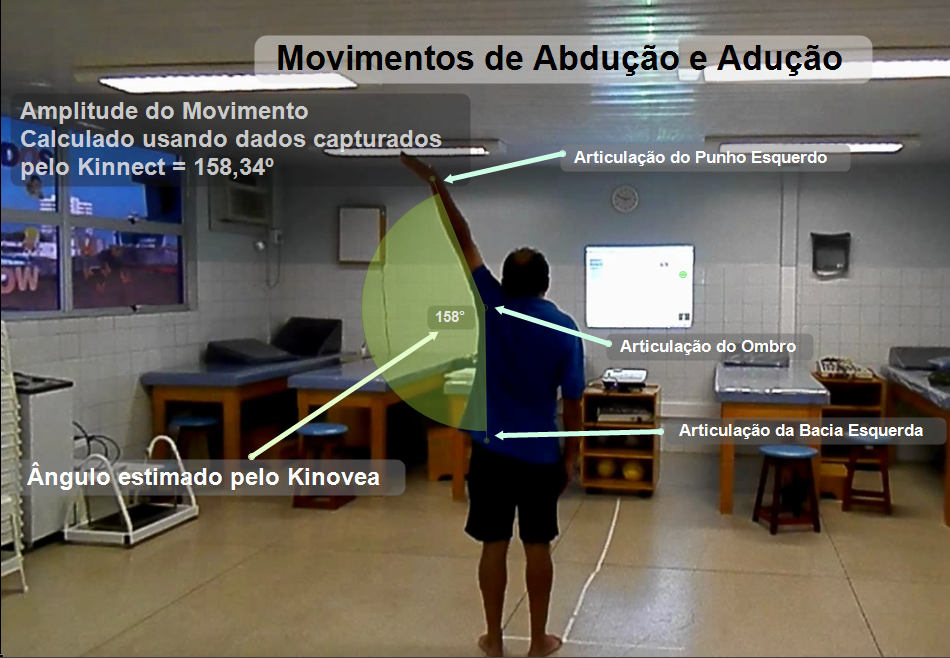
\includegraphics[scale=0.5]{./img/capturaducaokinnect.png}
 % matrixargseg.png: 296x162 pixel, 100dpi, 7.52x4.11 cm, bb=0 0 213 117
 %\caption{Estágio desenvolvimento de jogos ~\cite{fullerton2008game}}
\caption{Movimentos de Abdução e Adução}
%  \caption{Estágio desenvolvimento de jogos}
 \label{fig:movabducaomet}
\end{figure}

Durante a análise foram comparados os Ângulos Relativos do Tronco e do Levantamento de Braços dos Indivíduos. As grandezas cinemáticas coletadas nesses estudo foram:
\begin{enumerate}
	\item Do movimento de Abdução Figura \ref{fig:movabducaomet}, calculamos a amplitude máxima atingida por cada voluntário membros esquerdo e direito;
	\item Velocidade Angular de Abdução membros esquerdo e direito;
	\item Velocidade Angular de Adução membros esquerdo e direito.
\end{enumerate}

Esses dados biomecânicos foram coletados com o objetivo de identificar a bradicinesia nos indivíduos diagnosticados com a \ac{dp}ante os indivíduos sem o dianóstico da doença.
Pelo quantitativo da pesquisa ter sido de 27 indivíduos a abordagem de aprendizagem de máquina usando \ac{svm} ~\cite{vapnik95} foi utilizada juntamente com a técnica de validação-cruzada \textit{Leave One Out Cross-Validation} que será explicado com mais detalhes na \ref{chap:avaliacao}.


\subsection{Relação Risco e Benefício da Pesquisa}
Os riscos inerentes podem decorrer da exposição de dados dos sujeitos da pesquisa, o que pode acarretar danos morais e/ou psicológicos.

Assim, foram tomados todos os cuidados para que a identidade do sujeito da pesquisa não seja revelada, garantindo assim, privacidade e confidência das informações. Assim todos os dados do estudo foram manipulados apenas pelos principais pesquisadores, todos os dados serão armazenados sob criptografia, mitigando a possibilidade de vazamento da informação.

Caso ocorresse algum constrangimento por parte do sujeito da pesquisa, ao não conseguir realizar a pesquisa ou responder alguma pergunta devido ao comprometimento da doença. Os pesquisadores prestaram total assistência, orientando adequadamente os sujeito da pesquisa.

%Os presentes riscos fazem jus aos benefícios que a pesquisa venha a trazer com a possibilidade de monitoramento dos sintomas da \ac{dp}. A identificação dos sintomas motores e classificação desses dados através do computador podem permitir avanços para um melhor acompanhamento da evolução da doença além de possibilitar que os pacientes venham a ser monitorados de forma não invasiva através de um jogo eletrônico. Os pacientes deverão ter o seu estágio da \ac{dp} previamente diagnosticada por um médico para ser possível comparar os dados do monitoramento com a classificação obtida.




%\chapter{Entrevista Semi-Estruturada com Profissionais de Saúde}\label{chapter:entrevista_semi_estruturada}

A interpretação de dados é o cerne da pesquisa qualitativa. Esse método, tem como função desenvolver a teoria, servindo ao mesmo tempo de base para a decisão sobre quais dados adicionais devem ser coletados \cite{FLI04}. É importante que seja realizada a codificação seletiva, para que seja elaborada a categorização essencial sobre todas as categorias envolvidas \cite{FLI04}. O pesquisador precisa decidir quais os fenômenos salientes e ponderá-los de forma a ter como resultado uma categoria central juntamente com as categorias a ela relacionadas. O procedimento da interpretação dos dados, assim como a integração de material adicional, é encerrado quando atinge a "saturação teórica", quando o avanço da codificação não atinge mais novos conhecimentos \cite{FLI04}.

Para análise dos textos provenientes da pesquisa (transcrição da entrevista com os Neurologistas e Fisioterapeutas especialistas em Neurologia) foi utilizada a codificação seletiva através de criação de categorias a \emph{posteriori}. As categorias foram criadas e organizadas de acordo com o conteúdo de cada texto. As respostas de cada participante foram analisadas e a partir da identificação das categorias, incluídas na árvore de categorias do QDA Miner \cite{qda13}, que pode armazenar a transcrição de cada entrevista. Admitindo-se que uma classificação, para ser adequada não pode ser feita arbitrariamente, a categorização da árvore será criada e reformulada várias vezes, durante o processo de análise de acordo com o método de pesquisa\cite{FLI04}.


\subsubsection{Instrumento de Análise dos Dados da Pesquisa Qualitativa} \label{section:analise_dados} 
A pesquisa qualitativa assistida por computador \textit{software} permite a análise qualitativa das informações obtidas em modo texto
por intermédio do \textit{software} QDA Miner \cite{qda13}. Software dessa natureza auxiliam o pesquisador na organização dos registros da pesquisa e das interpretações dos mesmos. A escolha dessa ferramenta é justificada pela dificuldade de classificar e analisar os dados obtidos. Nessa análise somente foram levadas em consideração as atividades referentes ao acompanhamento dos sintomas motores em pacientes de parkinson e como um possível cenário que permita o monitoramento desses sintomas por intermédio de jogos eletrônicos poderia auxiliar os pacientes e também os profissionais de saúde.

Detalhamos a entrevista semi-estruturada realizada, descrevendo a opinião dos entrevistados e coletando requisitos baseado nas necessidades expostas pelos mesmos. Essa etapa da pesquisa é importante para testar a Hipótese \textbf{H1} usando pesquisa qualitativa para sua avaliação, que realizou uma análise do ponto de vista do profissional da saúde para a comprovação da hipótese:

	\begin{description}
	\item[H1] O acompanhamento de sintomas motores integrados à rotina diária do paciente, traz benefícios ao tratamento e qualidade de vida do mesmo, do ponto de vista do profissional da saúde.
	\end{description}
	
\subsection{Análise da Entrevista Semi-Estruturada}
Nesta seção são apresentados os resultados da Entrevista Semi-Estruturada como exposto na Figura \ref{figure:desenho_pesquisa}}.
A análise qualitativa ~\cite{FLI04} permitirá identificar as práticas dos profissionais de saúde referentes ao acompanhamento dos sintomas motores em pacientes de parkinson e como essas práticas podem ser aperfeiçoadas num cenário em que haja o monitoramento dos sintomas.

A identificação dos requisitos de um sistema representa o início da aquisição das necessidades da solução a ser proposta. Os requisitos definem quais serão os serviços que o sistema deverá prover além de um conjunto de restrições existentes na operação do mesmo \cite{sommerville2011}. Para Nuseibeh \cite{bas00}  a Engenharia de Requisitos é o processo de descobrir o propósito do software, identificando os principais envolvidos do sistema com suas respectivas necessidades e documentando a análise realizada para uma implementação posterior. Contudo, é um processo que deve ser continuamente repetido para que a necessidades dos envolvidos sejam satisfeitas. As técnicas para identificação de requisitos são derivadas principalmente das ciências sociais, que se baseiam em pesquisa qualitativa onde são analisados a teoria do objeto de estudo com a experiência prática dos envolvidos na pesquisa ~\cite{zowghi2005}. Uma das técnicas de identificação de requisitos baseada em pesquisa qualitativa é a entrevista semi-estruturada em que o entrevistador possui um conjunto de perguntas pré-definidas e guia a entrevista de acordo com a opinião do entrevistado ~\cite{FLI04}.


\section{Perfil dos Participantes}
Os participantes da pesquisa foram 4 profissionais de saúde onde 2 são Fisioterapeutas com especializações em Neurologia e 2 são médicos especialistas em Neurologia. A escolha do diferente perfil desses profissionais se fez necessária porque os ambos os profissionais desempenham funções distintas para o tratamento e acompanhamento dos pacientes da ~\ac{dp}. Os neurologistas realizam o diagnóstico e acompanham os sintomas motores juntamente com as informações obtidas do paciente ou cuidador realizando assim o gerenciamento da dosagem medicamentosa da doença. Por outro lado, os fisioterapeutas fazem o acompanhamento dos sintomas motores em sessões de fisioterapia promovendo a aprendizagem motora desses pacientes. Logo esses profissionais possuem visões e preocupações distintas inerentes a sua profissão. 


Para manter a confidencialidade de informação, os entrevistados irão receber uma Legenda que possa identificar unicamente o profissional sem revelar sua identidade como descrito na Tabela~\ref{table:perfil_analise_participantes}.

\begin{table}[h]
\caption{Perfil dos Participantes}
\label{table:perfil_analise_participantes}
\begin{tabular}{|l|l|c|c|}
\hline
\textbf{LEGENDA} & \textbf{PROFISSÃO}             & \multicolumn{1}{|l}{\textbf{IDADE (ANOS)}} & \multicolumn{1}{|l|}{\textbf{EXPERIÊNCIA (ANOS)}} \\ \hline
FIS\_01          & Fisioterapia em Neurologia & 40                                         & 10                                                \\ \hline
FIS\_02          & Fisioterapia em Neurologia     & 39                                         & 10                                                \\ \hline
NEU\_01          & Médico Neurologista            & 42                                         & 15                                                \\ \hline
NEU\_02          & Médico Neurologista            & 67                                         & 30                                                \\ \hline
\end{tabular}

\end{table}

\subsection{Questionário de Pesquisa}
Para a construção do questionário foi realizada uma análise sobre a doença de parkinson e sintomas que pudessem ser monitorados usando sensores, para a construção do questionário foram utilizadas diretrizes médicas da Doença de Parkinson ~\cite{protpar010,national2006parkinson} e da tabela UPDRS ~\cite{updrs87} usada para avaliação do progresso da doença ~\cite{updrs87}. Foram elaboradas 15 perguntas agrupadas em 3 seções Apêndice \ref{apendice:entrevista-semi-estruturada}, com os seguintes temas: sintomas da doença de parkinson, monitoramento da saúde motora e os benefícios advindos do monitoramento. Devido as diferenças existentes na abordagem utilizada por cada profissional o entrevistador pôde selecionar as questões de acordo com as habilidades e responsabilidades do entrevistado.

\section{Análise}
Durante a análise dos textos, alguns foram extraídos para demonstrar os fragmentos encontrados durante esta análise. A nomenclatura utilizada nos fragmentos encontrado nessa análise contém o prefixo \textbf{FRAGMENTO} mais um número sequencial identificando o mesmo. Esse procedimento visou identificar \textbf{requisitos} que orientem a proposta de monitoramento de dados motores por intermédio de jogos eletrônicos, no que se refere a definir parâmetros importantes para o monitoramento motor e a perspectiva do profissional de saúde em relação a abordagem apresentada nesta Proposta de Tese. Para a captura do requisito, ficou estabelecido que ele deve ser importante para os entrevistados onde cada requisito extraído das entrevistas será citado como \textbf{REQ-ENTREVISTAS}, seguido por um número correspondente à sequencia de sua apresentação.

\subsection{Diagnóstico}\label{section:analise_diagnostico}
Inicialmente durante a entrevista com os Médicos Neurologistas que são responsáveis pelo diagnóstico da \ac{dp} como é realizado o diagnóstico da \ac{dp}. Foi identificado tanto na literatura ~\cite{tolosa06,vedolin2003} quanto nas entrevistas a dificuldade de se obter um diagnóstico da \ac{dp}, pois atualmente ainda não existe um diagnóstico estabelecido da doença ~\cite{national2006parkinson,protpar010}. 

Todos os profissionais informaram que o sintoma mais comum é o tremor de repouso, que normalmente é unilateral e seguido de uma bradicinesia como podemos ver em ([FRAGMENTO-01][FRAGMENTO-02]). Ainda no ([FRAGMENTO-01]), existe uma ocorrência que a \textbf{[NEU\_01]} reforça em mais 4 oportunidades durante a entrevista, ressaltando a importância da técnica de \textit{Finger Taps} ~\cite{updrs87} para avaliação da bradicinesia sintomas na \ac{dp}.


\begin{quote}
\textbf{[FRAGMENTO-01][NEU\_01]} -
\emph{O diagnóstico da doença de Parkinson é quando o paciente chega se queixando de tremor. Esse sintoma começa com um tremor unilateral, geralmente pelas mãos, lentamente progressivo e de repouso. Além do tremor esse paciente exibe também uma lentidão que a gente consegue detectar pelo \textit{Finger Taps}. Que é colocando o polegar o primeiro e segundo dedo simultaneamente para ver se há ou não lentidão e comparando sempre com o outro lado você vai ver que há uma diferença. E existe também uma rigidez, quando você colocar o braço e faz uma flexão e extensão e você vê o tônus desse paciente comparado com o outro lado há uma diferença.}
\end{quote}

\begin{quote}
\textbf{[FRAGMENTO-02][NEU\_02]} -
\emph{
O diagnóstico da doença de Parkinson é feito com uma das queixa iniciais do paciente é um tremor de repouso geralmente associado a uma dificuldade na marcha. Os pacientes reclamam de uma perna presa e um tremor de repouso. 
}
\end{quote}

Um ponto que deve ser ressaltado no  ([FRAGMENTO-03]), é o que o entrevistado referiu como ``\textit{boa resposta ao prolopa}''. Essa ocorrência é chamado de diagnóstico diferencial da \ac{dp} ~\cite{protpar010}. Possivelmente com a abordagem utilizada nesta Proposta de Tese, poderíamos avaliar essa ocorrência e fornecer subsídios para que o profissional de saúde venha a decidir se a resposta à medicação foi efetiva e consequentemente realizar o diagnóstico diferencial.

\begin{quote}
\textbf{[FRAGMENTO-03][NEU\_01]} - 
\emph{
Então os sintomas é o tremor em repouso, a lentidão e a rigidez. De um lado só, por exemplo começa no braço direito e depois vai para a perna direita, depois para o braço esquerdo e depois a perna esquerda. Isso lentamente progressivo. E a gente faz a exclusão com outras doenças através de outros exames como tomografia, ressonância e com uma boa resposta ao prolopa.
}
\end{quote}

\subsection{Sintomas}
Nesta seção estão expostos a importância dos sintomas para o acompanhamento da sintomatologia da doença de parkinson do ponto de vista dos profissionais de saúde participantes da pesquisa.

\subsubsection{Tremor}
O sintoma de tremor além de ter sido referenciado durante o diagnóstico da doença ~\ref{section:analise_diagnostico} por todos os entrevistados. Contudo, este sintoma possui particularidades como a dificuldade de controlar o sintoma por intermédio do tratamento medicamentoso ([FRAGMENTO-04]). Outra aspecto que deve ser levado em consideração também nesse sintoma é que ele não é tão incapacitante quanto a bradicinesia ~\ac{dp} ([FRAGMENTO-05]), neste fragmento o [NEU\_01] reforça da importância de controlar os sintomas de lentidão do movimento ante os de tremor ~\cite{do2007parkinson}.

\begin{quote}
\textbf{[FRAGMENTO-04][NEU\_01]} - 
\emph{
Mas a gente tem que ver, porque as vezes o tremor é muito mais difícil de você controlar. Porque tem muito haver com a parte emocional. Quanto mais emocionalmente desequilibrado o paciente tiver, mais tremor ele tem.
}
\end{quote}

\begin{quote}
\textbf{[FRAGMENTO-05][NEU\_01]} - 
\emph{
O controle do tremor é um pouco complicado porque é um dos sintomas mais difíceis de ser controlado com as medicações  que temos hoje.  Então você poderia ver, principalmente nos seus exames seria a lentidão. Porque o paciente quer tremer mas ele não quer ficar lento.
}
\end{quote}


\subsubsection{Bradicinesia}\label{section:analise_bradicinesia}

O pesquisador indagou se o sintoma da bradicinesia era considerado o mais debilitante da ~\ac{dp} e como resposta ele obteve a afirmação que a bradicinesia impacta diretamente na qualidade de vida do paciente, privando-o de realizar as atividades diárias ([FRAGMENTO-06]).

\begin{quote}
\textbf{[FRAGMENTO-06][NEU\_01]} - 
\emph{
É ele atrapalha né, principalmente no levantar no andar, para você se levantar, pentear o cabelo e o tremor é prejudicial, mas mais prejudicial ainda é a lentidão do movimento.
}
\end{quote}


Ao indagar ao [NEU\_01] se o movimento de adução e abdução do braço, seria relevante para a identificação da~\ac{dp}, o profissional informou que a bradicinesia é um sintoma que traz lentidão em todo o corpo e possivelmente iria afetar nesse movimento também devido à redução dos movimentos automáticos ([FRAGMENTO-07]) que corrobora com a afirmação do [FIS\_01] que explica os impactos físicos de um paciente com a ~\ac{dp} ([FRAGMENTO-08]).

\begin{quote}
\textbf{[FRAGMENTO-07][NEU\_01]} - 
\emph{
Na verdade o movimento em si, vai ver o quão lento está. Porque você não tem um déficit motor. O comprometimento na doença de Parkinson está no comprometimento piramidal, o comprometimento extra-piramidal não vai estar alterando a força motora. O que vai estar vai ser exatamente a lentidão. A lentidão e o quão mais específico é que o paciente vai pegar naquele lugar. Por exemplo, é um paciente que está andando você que os movimentos dele automáticos estão reduzidos, principalmente no balançar dos braços. Você vai andando, vai andando, você vê aquele paciente que está com a força, ele está com toda a estrutura piramidal tudo normal. Mas ela anda lento em consequência da lentidão do movimento porque os movimentos automáticos estão reduzidos.
}
\end{quote}


\begin{quote}
\textbf{[FRAGMENTO-08][FIS\_01]} - 
\emph{
Os sintomas mais frequentes a gente tem a bradicinesia que é a lentificação do movimento, a gente tem um padrão postural que começa a ficar bem nítido que o paciente apresentar o Parkinson que é uma perda da movimentação automática da cintura escapular e aí ele começa a apresentar uma diminuição no volume da voz que é uma dipofonia e ele começa a apresentar uma maior rigidez muscular, que eles reclamam bastante e a bradicinesia que tornam os movimentos cada vez mais lentos.
}
\end{quote}



\subsubsection{Marcha}

Encontramos uma menção à dificuldade de andar do paciente de ~\ac{dp}, quando o [NEU\_01] cita no ([FRAGMENTO-07]) (``\textit{Você vai andando, vai andando, você vê aquele paciente que está com a força, ele está com toda a estrutura piramidal tudo normal. Mas ela anda lento em consequência da lentidão do movimento ...}''. O [NEU\_02] corrobora com a mesma opinião ao citar a dificuldade de iniciar a marcha no ([FRAGMENTO-09]).
Por outro lado, o fisioterapeuta tem o papel de realizar o acompanhamento da marcha nas sessões de fisioterapia além de fornecer um aprendizado motor para a melhora da qualidade de vida do paciente de acordo com suas limitações devido a sintomatologia da doença como podemos ver no ([FRAGMENTO-10]).

\begin{quote}
\textbf{[FRAGMENTO-09][NEU\_02]} - 
\emph{
Problema na marcha. Dificuldade de iniciar a marcha, certa dificuldade de um lado comprometido. Mesmo quando o sintoma está unilateral eles sentem dificuldade para iniciar a marcha.
}
\end{quote}

\begin{quote}
\textbf{[FRAGMENTO-10][FIS\_01]} - 
\emph{
Numa marcha, o doente de Parkinson tem a tendência de estar olhando para o chão. Mas a gente sabe que isso não é compatível com uma boa marcha a tendência é cair, para piorar eles têm os passos miúdos e também um passo arrastado, então esse passo favorece a queda. Então, ele perdeu a marcha automática que é aquele que a gente adquire na infância. A gente vai evoluindo vai levando as nossas quedas  corrige.  O doente, ele perde isso. O que a gente faz nas sessões de fisioterapia é tentar aplicar auto-correções para adaptar o paciente à nova realidade para que ele tenha uma aprendizado motor e no futuro um automatismo do movimento.
}
\end{quote}

Devido a essa recorrência de opiniões sobre a importância da análise da marcha ~\ref{section:analise_marcha} para o acompanhamento dos sintomas da doença de Parkinson, esse trabalho que realizou um estudo mais aprofundado desse movimento na Seção~\ref{section:analise_marcha_pca}. Um detalhe importante que tem haver com a integridade física dos sujeitos da pesquisa é a possibilidade de queda como encontrado no [FRAGMENTO-10] \textit{``Mas a gente sabe que isso não é compatível com uma boa marcha a tendência é cair ...''} que vai além do do custo financeiro para a aquisição dos sensores de que capturam a~\ac{fvrs} ~\cite{dyno}) e reforça a importância de bases de dados motoras como a Physionet~\cite{physionet} com o intuito de preservar a integridade física dos pacientes.



\subsection{Monitoramento Motor}
Nesta seção estão expostos a importância do monitoramento dos sinais capturados durante a pesquisa no estudo analítico de caso controle exposto no Método de Pesquisa na Seção ~\ref{section:estudo_caso_controle}. Nesse estudo também pretendemos identificar características dos movimentos que possam ser extraídos desses sinais e que venham fornecer subsídios para diferenciar indivíduos diagnosticados com a ~\ac{dp} ante indivíduos sem o diagnóstico da doença.

\subsubsection{Amplitude do Movimento dos Braços}

Ao indagar ao [FIS\_02] se o movimento de adução e abdução do braço seria relevante para a identificação da ~\ac{dp} o fisioterapeuta informou que mesmo não sendo um teste específico para a identificação da doença, existiam diferenças significativas encontradas em indivíduos diagnosticados com parkinson [FRAGMENTO-11].
\begin{quote}
\textbf{[FRAGMENTO-11][FIS\_02]}-
\emph{
Sim. Existe alterações sim, mas eu nunca vi especificamente esse teste como sendo usado para diagnóstico da doença. Mas que realmente existem mudanças no movimento de adução e abdução de uma pessoa normal ante a um parkinsoniano.
}
\end{quote}

O [FIS\_01], explicou os motivos que levam a perda da mobilidade no movimento de adução e abdução ([FRAGMENTO-12]) e consequentemente, reforça que esse movimento poderia ser monitorado para verificarmos o comprometimento da doença. Em um outro fragmento ([FRAGMENTO-13]) o mesmo fisioterapeuta reforça da importância de monitorar a amplitude do movimento, pois permite visualizar a resposta do paciente ao tratamento oferecido.

\begin{quote}
\textbf{[FRAGMENTO-12][FIS\_01]}-
\emph{
Têm, porque uma das grandes perdas que eles apresentam é na cintura escapular e consequentemente é pegando a parte de ombro. Pois caso ela seja mais fixa, porque geralmente o paciente de Parkinson abduz o ombro. O ombro fica abduzido junto ao tronco e ai ele perde a mobilidade do cotovelo e punho e também o movimento fica comprometido por conta disso.
}
\end{quote}

\begin{quote}
\textbf{[FRAGMENTO-13][FIS\_01]}-
\emph{
Mesmo sabendo que a tendência é uma lentificação (bradicinesia).  As outras doenças também, porque um dos objetivos nossos é o aumento da amplitude. Então é um meio interessante para a gente conseguir visualizar se o tratamento está dando certo ou não.
}
\end{quote}



\subsubsection{Velocidade do Movimento De Adução e Abdução dos Braços}
Um ponto de convergência entre os profissionais foi a importância de monitorar a velocidade angular dos pacientes. Pois os profissionais tentam convergir o tratamento fisioterápico e medicamentoso para a melhora do sintoma da bradicinesia, então para os profissionais a melhora está condicionada a um aumento na velocidade do movimento ([FRAGMENTO-14],[FRAGMENTO-15])

\begin{quote}
\textbf{[FRAGMENTO-14][NEU\_01]} - 
\emph{
É como eu falei para mim seria melhor se capturássemos se ele está mais lento. Se através dessa amplitude você conseguir por intermédio do computador identificar que ele está mais lento de um lado do que do outro. Conseguir visualizar a velocidade de um lado e do outro, então isso é interessante.
}
\end{quote}


\begin{quote}
\textbf{[FRAGMENTO-15][FIS\_01]} - 
\emph{
É e consequentemente a velocidade, porque nesse caso o tratamento é diretamente relacionado a isso quanto mais veloz o parkinsoniano é melhor para a gente melhor prognóstico a gente pode ter lá na frente. Mesmo sabendo que a tendência é uma lentificação.
}
\end{quote}




\subsubsection{Assimetria do Movimento}

A assimetria do movimento acomete os pacientes que estão nos estágios iniciais da doença. Por esse motivo, geralmente ele é  identificado durante o diagnóstico [FRAGMENTO-03]. Porém, alguns pacientes parkinsonianos persistem com a assimetria do movimento em que um dos lados é mais comprometido que o outro. Por esse motivo é que o [NEU\_01] afirmou \textit{``Se através dessa amplitude você conseguir por intermédio do computador identificar que ele está mais lento de um lado do que do outro.}. Porque a tendência natural da evolução da doença de parkinson é que haja redução na assimetria do movimento conforme a opinião do [NEU\_01] no [FRAGMENTO-16] e a Tabela UPDRS em sua escala de avaliação do progresso da doença ~\cite{updrs87} (Seção ~\ref{section:escalas_avaliacao}).

\begin{quote}
\textbf{[FRAGMENTO-16][NEU\_01]}-
\emph{
No início. Geralmente o paciente se queixa de uma diminuição de força de um lado do corpo. Mas na progressão, ele vai sentir dificuldade global. Mas aqueles parkinsonianos iniciais geralmente eles se queixam na diminuição do movimento de um dos lados.
}
\end{quote}

\subsection{Benefícios Advindos do Monitoramento}


\subsubsection{Quantificação dos Sintomas}
As perguntas relacionadas à quantificação dos sintomas como amplitude de movimento, velocidade angular e se seria válido acompanhar esses valores para o monitoramento dos sintomas. Nos trouxe dois grupos de respostas, uma que reconhecia da importância da quantificação dos dados para poder mensurar a melhora ou piora do paciente de forma quantitativa como está no [FRAGMENTO-17]. E outra resposta é que esses valores teriam mais validade científica do que prática, pois na prática os profissionais já monitoram esses sintomas manualmente [FRAGMENTO-18]. Todavia, se esses profissionais tivessem acesso a um sistema que permitisse o monitoramento motor e consequentemente conseguissem perceber os seus benefícios. Esses mesmos profissionais poderiam modificar a prática atual de forma manual e adotar uma nova proposta.

\begin{quote}
\textbf{[FRAGMENTO-17][FIS\_02]}-
\emph{
É preciso ter parâmetros sim. Pois atualmente usamos muito o olho clínico e ai vai de cada profissional. Se tivermos números facilitam bastante porque se tornam fatos e basearmos nossas conclusões em números é bem melhor.
}
\end{quote}

\begin{quote}
\textbf{[FRAGMENTO-18][FIS\_01]}-
\emph{
É interessante em termos de pesquisa. Em termos de clínica a geralmente a gente vai no geral. Por exemplo: Eu faço uma flexão de ombro com bastão e anotei no meu exame que ele ia até mais ou menos 70º e após 15 dias eu vejo que ele está levantando acima de 90º. Então está marcado a minha evolução. Então eu faço a avaliação nesse sentido. Então esse sistema seria bom para pesquisa mesmo.
}
\end{quote}



\subsubsection{Gerenciamento da Dosagem Medicamentosa}
O monitoramento dos dados motores poderia ser bastante utilizado no gerenciamento da dosagem medicamentosa. Os profissionais sentem a necessidade de visualizar a eficácia de seu tratamento junto ao paciente. O [FIS\_01] no [FRAGMENTO-19] cita a importância de avaliar tanto o tratamento medicamentoso quanto se a sua atividade fisioterápica está trazendo benefícios ao paciente. Os Neurologistas citam ([NEU\_01] e [NEU\_01]), citam a importância de reajustar a dosagem medicamentosa e que poderiam visualizar se o medicamento estaria surtindo efeito no paciente. Outra opinião bastante pertinente é que o agravamento da ~\ac{dp} é bastante sutil segundo a [NEU\_01] no [FRAGMENTO-21], logo se houvesse fosse possível mostrar a evolução da doença em períodos mais longos o tratamento poderia ser mais efetivo e consequentemente melhoraria a qualidade de vida dos pacientes.


\begin{quote}
\textbf{[FRAGMENTO-19][FIS\_01]} - 
\emph{
 É interessante porque teremos uma ideia de até que ponto a medicação está sendo efetiva, até quando a patologia está progredindo e também avaliar se o nosso tratamento fisioterápico está dando resultados ao tentar frear a evolução da doença.
}
\end{quote}


\begin{quote}
\textbf{[FRAGMENTO-20][NEU\_02]} - 
\emph{
Sim. Dentro do que você propõe. Com certeza sim. Essa avaliação desses movimentos. Porque a gente consegue visualizar se a medicação está surtindo efeito, se precisa ser reajustada.
}
\end{quote}

\begin{quote}
\textbf{[FRAGMENTO-21][NEU\_01]} - 
\emph{
Se esse mecanismo acontecesse. Você poderia avaliar a dosagem de um paciente por exemplo. Veja avalie durante uma semana, não melhorou. Então a gente poderia fazer um teste com tremor, lentidão e a rigidez, se houvesse esse aspecto.  A gente poderia aumentar a dosagem e visualizaria a eficácia da dosagem com o decorrer do tempo, com o decorrer da evolução. E verificaria se realmente o paciente está melhorando. Porque o paciente da doença de Parkinson ele piora lentamente, as vezes é tão sutil que o próprio paciente não consegue. Então é como eu disse, cada paciente a evolução é diferente num existe. Mas poderia assim, se você conseguisse detectar as amplitudes do tremor por exemplo.
}
\end{quote}






\section{Requisitos Identificados}


%O uso do termo "Engenharia" implica que técnicas sistemáticas e repetidas devem ser aplicadas para certificar que os requisitos de um sistema estejam completos, consistentes e relevantes \cite{sommerville2011}. O emprego correto da Engenharia de Requisitos é um passo fundamental para o desenvolvimento de um bom  produto, onde a satisfação do usuário deve ser o principal objetivo a ser atingido \cite{zowghi2005}.
Os requisitos obtidos durante as fases de análise que compõem o processo de pesquisa descrito neste trabalho indicam a importância de monitorar os dados motores para uma avaliação posterior do profissional de saúde.
Para demonstrar a relevância do requisito identificado confrontamos a teoria com o que é aplicado na prática pelos profissionais de saúde. Por isso ao lado dos requisitos iremos citar referências científicas que corroboram com esses requisitos. 

\begin{description}
	\item[REQ-ENTREVISTAS-01 :] Identificar e quantificar o tremor parkinsonianno ~\cite{tolosa06,keijsers2006,lemoyne2010}.
	\item[REQ-ENTREVISTAS-02 :] Identificar a bradicinesia ~\cite{patel_monitoring_2009}. %Para identificar a bradicinesia pode ser calculada a velocidade angular do movimento de abdução e adução do braço.
	\item[REQ-ENTREVISTAS-03 :] Avaliar bradicinesia usando ~\textit{finger-tapping} ~\cite{finger2012}.
	\item[REQ-ENTREVISTAS-04 :] Considerar e identificar a assimetria do movimento nos estágios iniciais ~\cite{national2006parkinson}.	%Além da velocidade angular podemos calcular a amplitude do movimento, assim identificarems a assimetria do movimento com mais clareza.
	\item[REQ-ENTREVISTAS-05 :] Fornecer mecanismos para possibilitar o Diagnóstico Diferencial \cite{protpar010} da Doença de Parkinson. %caso os sintomas de bradicinesia e marcha sejam identificados. Caso os indivíduos venham a surtir efeito ao medicamento e consequentemente reduzir a gravidade do sintoma, então foi possível realizar um diagnóstico diferencial.
	\item[REQ-ENTREVISTAS-06 :] Analisar a Marcha ~\cite{gaitusingsensorsreview2012}. Medir a marcha e comparar o padrão do movimento com indivíduos com e sem o diagnóstico da ~\ac{dp} para classificar a marcha como saudável ou parkinsoniana.
	\item[REQ-ENTREVISTAS-07 :] Calcular e armazenar a amplitude do movimento de adução e abdução dos braços. Para realizar o monitoramento da saúde motora e poder acompanhar o tratamento.
	\item[REQ-ENTREVISTAS-08 :] Calcular e armazenar a velocidade angular do movimento de adução e abdução dos braços. Para poder avaliar o sintoma da bradicinesia.
	\item[REQ-ENTREVISTAS-09 :] Avaliar estado emocional e avaliar o comprometimento do tremor. 
\end{description}



\subsection{Inviabilidade Técnica}
Algumas requisitos identificados, atualmente devido a tecnologia do sensor de movimento utilizado atualmente é inviável sua implementação como:
\begin{itemize}
  \item O \textbf{REQ-ENTREVISTAS-01}, o tremor de repouso é um dos principais sintomas da doença de parkinson. Sabíamos da sua importância e desenvolvemos até um jogo para \textit{Smartphone} para tentar quantificar o tremor. Porém, ao testar junto aos usuários percebemos que ao usarem o jogo eles paravam de tremer inviabilizando a quantificação do tremor. 
	Contudo, ao realizar a coleta dos dados com pacientes de parkinson identificamos que alguns deles tremiam a mão que não estava em movimento. Ou seja, quando solicitávamos para abduzir o braço direito em alguns pacientes a mão esquerda tremia. Devido o tempo e o objeto de estudo que era o próprio movimento não avaliamos ainda o sinal produzido do braço parado.
	\item O \textbf{[REQ-ENTREVISTAS-03]}, a técnica de \textit{finger-tapping} não pode ser avaliadas utilizando o MS-Kinnect 1.0, pois nessa versão não existe a captura do movimento dos dedos conforme na Figura~\ref{fig:articulacoeskinnect} e consequentemente inviabiliza o seu monitoramento.
	\item O \textbf{REQ-ENTREVISTAS-09}, por envolver estado emocional e parâmetros que não estamos levando em consideração nesse trabalho esse requisito está fora do escopo deste trabalho. Porém com mecanismos de detecção de batimentos cardíacos presente em versões mais atuais do MS-Kinnect poderia averiguar a relação dos batimentos cardíacos com o tremor em trabalhos futuros.
\end{itemize}

\subsection{Matriz Rastreabilidade - Fragmento x Requisitos}
Essa Matriz de Rastreabilidade (Fragmento x Requisitos) vai mapear os \textbf{REQUISITOS} aos \textbf{FRAGMENTOS} que de forma direta ou indireta estejam correlacionados (Tabela \ref{table:matrix_rastreabilidade}). Ao final da matriz, temos um campo de Quantidade de Ocorrências que conta quantas vezes aquele requisito foi citado nos fragmentos.

%\begin{center}
\begin{table}[!htbp]
\caption{Matriz Rastreabilidade: Fragmento x Requisitos}
\label{table:matrix_rastreabilidade}
\begin{tabular}{||p{6.06cm}||ccccccccc|}
\hline
 \multicolumn{1}{|p{6.06cm}|}{\centering \textbf{FRAGMENTOS / REQUISITOS}} &  01 &  02 &  03 &  04 &  05 &  06 &  07 &  08 & 09 \\ 
\hline 
 \multicolumn{1}{|p{6.06cm}|}{\centering 01} &  x &  x &  x &  x &   &   &   &   &  \\ 
 \multicolumn{1}{|p{6.06cm}|}{\centering 02} &  x &   &   &   &   &  x &   &   &  \\ 
 \multicolumn{1}{|p{6.06cm}|}{\centering 03} &  x &  x &   &  x &  x &   &   &   &  \\ 
 \multicolumn{1}{|p{6.06cm}|}{\centering 04} &  x &   &   &   &   &   &   &   & x \\ 
 \multicolumn{1}{|p{6.06cm}|}{\centering 05} &  x &  x &   &   &   &   &   &   &  \\ 
 \multicolumn{1}{|p{6.06cm}|}{\centering 06} &   &  x &   &   &   &  x &   &   &  \\ 
 \multicolumn{1}{|p{6.06cm}|}{\centering 07} &   &  x &   &   &   &  x &  x &  x &  \\ 
 \multicolumn{1}{|p{6.06cm}|}{\centering 08} &   &  x &   &   &   &  x &  x &  x &  \\ 
 \multicolumn{1}{|p{6.06cm}|}{\centering 09} &   &   &   &  x &   &  x &   &   &  \\ 
 \multicolumn{1}{|p{6.06cm}|}{\centering 10} &   &   &   &   &   &  x &   &   &  \\ 
 \multicolumn{1}{|p{6.06cm}|}{\centering 11} &   &   &   &   &   &   &  x &   &  \\ 
 \multicolumn{1}{|p{6.06cm}|}{\centering 12} &   &  x &   &   &   &   &  x &  x &  \\ 
 \multicolumn{1}{|p{6.06cm}|}{\centering 13} &   &   &   &   &   &   &  x &   &  \\ 
 \multicolumn{1}{|p{6.06cm}|}{\centering 14} &   &  x &   &   &   &   &   &   &  \\ 
 \multicolumn{1}{|p{6.06cm}|}{\centering 15} &   &  x &   &  x &   &   &   &  x &  \\ 
 \multicolumn{1}{|p{6.06cm}|}{\centering 16} &   &   &   &  x &   &   &   &   &  \\ 
 \multicolumn{1}{|p{6.06cm}|}{\centering 17} &   &   &   &   &   &   &   &   &  \\ 
 \multicolumn{1}{|p{6.06cm}|}{\centering 18} &  x &   &  x &  x &   &  x &  x &  x & x \\ 
 \multicolumn{1}{|p{6.06cm}|}{\centering 19} &  x &   &   &   &  x &  x &  x &  x &  \\ 
 \multicolumn{1}{|p{6.06cm}|}{\centering 20} &  x &   &   &   &  x &  x &  x &  x &  \\ 
 \multicolumn{1}{|p{6.06cm}|}{\centering 21} &  x &   &   &   &  x &  x &  x &  x &  \\ 
\hline 
 \multicolumn{1}{|p{6.06cm}|}{\centering \textbf{QTD. OCORRÊNCIAS}} &  9 &  9 &  2 &  6 &  4 &  10 &  9 &  8 & 2 \\ 
\hline 
\end{tabular}
\end{table}
%\end{center}

\subsection{Matriz Rastreabilidade - Requisitos x Implementação}
Essa Matriz de Rastreabilidade (Requisitos x Implementaçao) vai mapear os \textbf{REQUISITOS} ao trabalho desenvolvido nessa Proposta de Tese. Isso demonstra o \textit{status} do trabalho e pode direcionar também os trabalhos futuros.

% Please remember to add \use{multirow} to your document preamble in order to suppor multirow cells
% Please remember to add \use{multirow} to your document preamble in order to suppor multirow cells
\begin{table}[!htbp]
\center
\begin{tabular}{|l|c|c|c|}
\hline
\multirow{\textbf{REQUISITO}} & \multicolumn{1}{|l}{\multirow{\textbf{SIM}}} & \multicolumn{1}{|l}{\multirow{\textbf{NÃO}}} & \multicolumn{1}{|l|}{\multirow{\textbf{\begin{tabular}[c]{@{}c@{}}AVERIGUAÇÃO\\ FUTURA\end{tabular}}}} \\
                                    & \multicolumn{1}{|l}{\textbf{}}                     & \multicolumn{1}{|l}{\textbf{}}                     & \multicolumn{1}{|l|}{\textbf{}}                                                                              \\ \hline
REQ-ENTREVISTA-01                   &                                                    &                                                    & X                                                                                                            \\ \hline
REQ-ENTREVISTA-02                   & X                                                  &                                                    &                                                                                                              \\ \hline
REQ-ENTREVISTA-03                   &                                                    & X                                                  &                                                                                                              \\ \hline
REQ-ENTREVISTA-04                   & X                                                  &                                                    &                                                                                                              \\ \hline
REQ-ENTREVISTA-05                   & X                                                  &                                                    &                                                                                                              \\ \hline
REQ-ENTREVISTA-06                   & X                                                  &                                                    &                                                                                                              \\ \hline
REQ-ENTREVISTA-07                   & X                                                  &                                                    &                                                                                                              \\ \hline
REQ-ENTREVISTA-08                   & X                                                  &                                                    &                                                                                                              \\ \hline
REQ-ENTREVISTA-09                   &                                                    & X                                                  &                                                                                                              \\ \hline
\end{tabular}
\end{table}

%\subsection{Requisitos de Jogos Com o Propósito de Monitoramento de Dados Motores}
%Nessa seção serão apresentados requisitos identificados durante a análise qualitativa da Entrevista Semi-Estruturada realizada com os profissionais de saúde conforme a metodologia de pesquisa. Para uma melhor análise dos resultados as considerações identificadas durante a análise foi confrontada com as diretrizes médicas ~\cite{protpar010,Jankovic_2008,ambulatoryparkinson2010} e a revisão da literatura sobre jogos para saúde \ref{section:jogos_saude} que serviram de base científica para esse trabalho.
%
%\subsubsection{Requisitos Essenciais}
%\begin{description}
	%\item[RE-001: – Progresso do jogo]
	%\item[RE-002: 
%\end{description}

%Requisitos Essenciais
%[RE-001] – Progresso do jogo
%Segundo Suhonnen, a característica mais atrativa de um jogo é perceber o progresso do mesmo. É o usuário conseguir visualizar o progresso do jogo [8].
%[RE-002] – Estado de Fluxo ou Escapismo
%O jogador tem que sentir relaxado e com desejo de repetir a atividades em outras oportunidades [8], o jogo tem que permitir que o usuário entre num estágio de fluxo [20] e execute as atividades sem perceber a noção de tempo e espaço. O usuário deverá jogar pelo próprio prazer.
%[RE-003] – Pontuação e Taxas de Acerto
%O jogador deve visualizar suas ações positivas e negativas. O jogo deverá pontuar as atividades do jogador de acordo com seus acertos. O jogador deve visualizar claramente os objetivos e perceber o sucesso ou fracasso alcançado [8], [15].
%[RE-004] – Preocupação física do jogador
%Por promover atividades físicas, ou ações que possam trazer injúria ao jogador, como movimentos de equilíbrio, movimentos repetitivos ou rápidos. O game design do jogo deve ter a preocupação de desenvolver o jogo de acordo com o público-alvo. Isso significa dizer que a faixa etária e limitações físicas e cognitivas em decorrência da idade ou enfermidade devem ser levadas em consideração. Os jogadores devem ter a segurança de usarem o jogo e ter a certeza que o seu uso não acaarretará em nenhum dano físico [1].
%[RE-004] – Monitoramento dos sinais vitais
%O jogo poderá monitorar os sinais vitais através dos sensores usados como interface do jogo. Sensores de movimento, podem ser aplicados para movimentar o personagem. Monitores cardíacos para controlar a intensidades dos exercícios físicos. Eletroencefalograma podem ser usados para acompanhar o nível de concentração do jogador [15]. A partir dos dados capturados, estes podem ser armazenados para uma avaliação a posteriori por um profissional de saúde. Desta maneira teremos um monitoramento dos dados de saúde de maneira não invasiva e presente na rotina do usuário.
%Requisitos Secundários
%[RS-001] – Motivar atividade física
%Os jogos para monitoramento de saúde que fazem uso de sensores de movimento, normalmente mootivam a prática de exercícicio físico [1], [8], [15]. Logo, esse requisito pode ocorrer de forma secundária sem ser o propósito principal do jogo.
%[RS-002] – Promover Reabilitação
%Para alguns tipos de usuário o jogo poderá ser usado para reabilitação. Usuários que tenham passado por acidentes vascular cerebral, cirurgia recente em algum membro. Estudos indicam que os jogos para exercício físico podem ser aplicados para auxiliar a reabilitação do usuário. Então como requisito secundário poderia atender a esse fim.
%[RS-003] – Adequação ao Tratamento
%Através da abordagem do jogo será possível influenciar o jogador a uma maior aderência ao tratamento[13], [14]. Contudo essa abordagem é difícil de ser adequada para um jogo voltado ao entretenimento.

\section{Conclusão}
Como dito no início do capítulo, buscamos nessa entrevista semi-estruturada avaliar a Hipótese \textbf{H1} da presente Proposta de Tese. Com este intuito, verificamos junto aos profissionais de saúde que um sistema de monitoramento de dados motores traria benefícios a qualidade de vida dos pacientes

Segundo o acompanhamento de sintomas motores integrados trazem benefícios no tratamento dos pacientes e como consequência uma melhora na qualidade de vida, do ponto de vista do profissional da saúde. Com base na rastreabilidade dos fragmentos da entrevista e a respectiva identificação dos requisitos. Pudemos concluir que houve muitas ocorrências nos requisitos de Identificação de sintomas como : tremores ([\textbf{REQ-ENTREVISTAS-01}]), bradicinesia [\textbf{REQ-ENTREVISTAS-02}] e análise da marcha [\textbf{REQ-ENTREVISTAS-06}]; para o acompanhamento e monitoramento da doença os profissionais de saúde também citaram da importância de calcular tanto a amplitude dos movimentos ([\textbf{REQ-ENTREVISTAS-07}]) quanto a velocidade angular da abdução e adução dos braços ([\textbf{REQ-ENTREVISTAS-08}]). Baseado nessas considerações, podemos validar qualitativamente a Hipótese \textbf{H1} como propõe o método de pesquisa utilizado nesta Proposta de Tese (Seção \ref{sec:desenho_pesquisa}).

\chapter{Arquitetura de Software para \textit{GAHME}}\label{chapter:arquitetura_captura}

A arquitetura do sistema faz uso de diferentes tecnologias conforme a Figura~\ref{fig:arquitetura}. Essa arquitetura facilita o desenvolvimento de um jogo para monitoramento de dados por criar uma camada de \textit{software} integrada a uma \textit{engine} de jogos bem conhecida e bastante utilizada pelas desenvolvedoras de jogos. Com o propósito de facilitar a programação de jogos para saúde e ser aplicados em outros contextos, foi criado um Componente de \textit{Software} sobre a \textit{engine} de jogos Unity 3D~\cite{unity3d}. Desta maneira, desenvolvedores de jogos podem criar \textit{GAHMEs} usando esse arcabouço (Seção~\ref{sec:cliente_game}) abstraindo da complexidade existente no processamento do sinal dos dados e na identificação dos sintomas motores. 

\begin{figure}[!htbp]
 \centering
 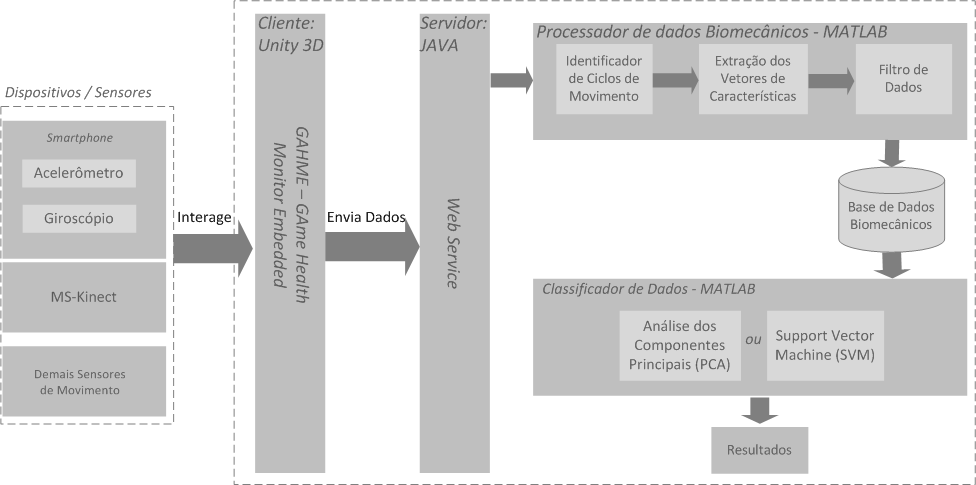
\includegraphics[scale=0.4]{./img/arquitetura}
 % matrixargseg.png: 296x162 pixel, 100dpi, 7.52x4.11 cm, bb=0 0 213 117
 %\caption{Estágio desenvolvimento de jogos ~\cite{fullerton2008game}}
\caption[Extensão da Arquitetura do Sistema Proposta por Santos Jr.]{Extensão da Arquitetura do Sistema Proposta por Santos Jr. ~\cite{antonio2013}}
%  \caption{Estágio desenvolvimento de jogos}
 \label{fig:arquitetura}
\end{figure}

\section{Aquisição de Dados}
A arquitetura Cliente e Servidor do \textit{GAHME} foi realizada com a colaboração de um ex-aluno de Mestrado da UFCG  Antônio Santos Jr. ~\cite{antonio2013} esta seção contém parte de seu trabalho.

\subsection{Arquitetura do Cliente \textit{GAHME}}\label{sec:cliente_game}
O Unity3D ~\cite{unity3d} é um ambiente de desenvolvimento de jogos multi-plataforma. Isso permite que os desenvolvedores possam abstrair aspectos do Hardware em que o jogo será executado tendo a preocupação somente com o desenvolvimento do jogo, após desenvolvido eles podem ser portados para \textit{Web}, \textit{Desktop},PCs, \textit{Smartphone} e até mesmo consoles de jogos eletrônicos ~\cite{unitysue}.

Atualmente, desenvolvedores independentes de jogos utilizam Unity3D como ferramenta de desenvolvimento, pois esse ambiente facilita a criação de: cenários dos jogos, terrenos, interação com os objetos usando uma linguagem de \textit{Script}. Desta maneira, nos últimos anos ocorreu uma popularização do desenvolvimento de jogos eletrônicos independentes.  Contudo, o desenvolvimento com propósito de monitorar dados motores possui desafios que não necessariamente precisam ser repassados para os desenvolvedores de jogos. Por esse motivo, criou-se um Arcabouço de \textit{software} herdando de um componente do Unity3D chamado Zigfu~\cite{zigfu} que permite integrar o Ms-Kinnect ~\cite{kinnect2013} como controlador do jogo. 

Os jogos eletrônicos que fazem uso dos movimentos do corpo permitem a liberdade de movimento, logo o movimento exercido nestes possibilitam muita variabilidade. Logo, é necessário que o desenvolvedor tenha a informação de quais ações o jogador precisa executar para que estas sejam monitoráveis. As ações de um \textit{GAHME} devem estar descritas no \textit{GAHME Action Design} (Seção~\ref{subsec:game_actions_guide}) como estabelecido no processo de desenvolvimento proposto no Capítulo~\ref{chap:processo_desenvolvimento}.

O Ms-Kinnect ~\cite{kinnect2013} é um sensor de captura de movimentos utilizado tanto para o console MS-XBOX 360 quanto para \textit{PCs}. Ele consegue capturar o movimento do corpo humano, e identificar as articulações por meio da posição anatômica do corpo humano~\cite{hamill1999bases}, como pode ser visto na Figura~\ref{fig:articulacoeskinnect}.

\begin{figure}[!htbp]
 \centering
 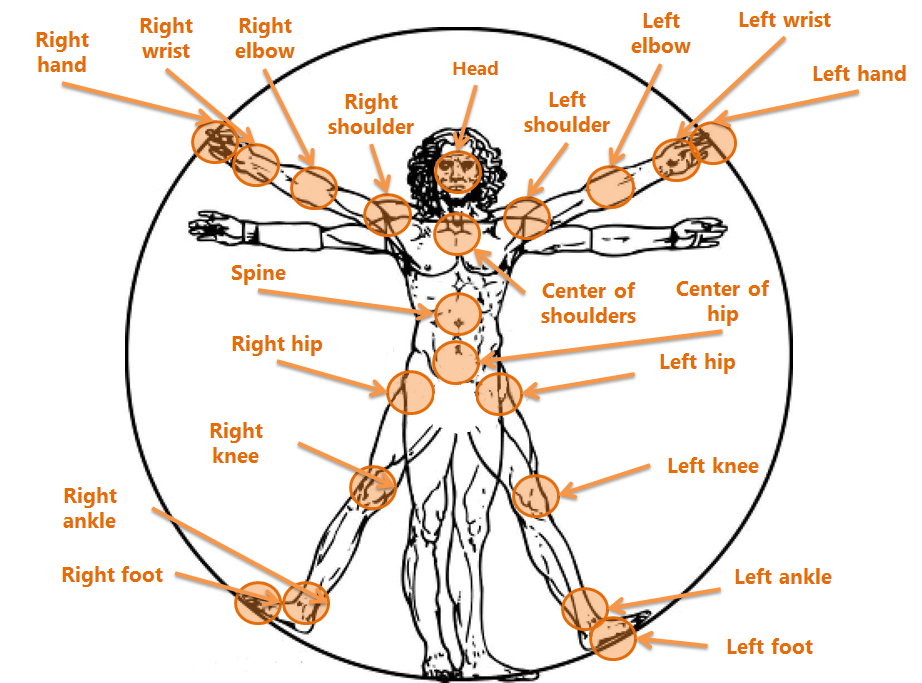
\includegraphics[scale=0.4]{./img/articulacoes.png}
 % matrixargseg.png: 296x162 pixel, 100dpi, 7.52x4.11 cm, bb=0 0 213 117
 %\caption{Estágio desenvolvimento de jogos ~\cite{fullerton2008game}}
\caption[Posições das Articulações do Corpo Humano Adquiridas Pelo MS-Kinnect]{\copyright Posições das Articulações do Corpo Humano Adquiridas Pelo MS-Kinnect ~\cite{kinnect2013}}
%  \caption{Estágio desenvolvimento de jogos}
 \label{fig:articulacoeskinnect}
\end{figure}

O Zigfu ~\cite{zigfu} é um componente de Software que permite integrar o Ms-Kinnect ao Unity3D. O Zigfu faz um mapeamento das articulações adquiridas pelo Ms-Kinnect (Figura~\ref{fig:articulacoeskinnect}) para uma classe chamada \textit{ZigSkeleton} com todas as articulações como podemos ver no Diagrama de Classe (Figura~\ref{fig:diagramaclassezigfu}). No entanto, para adquirir os sinais motores é necessário armazenar os valores das posições das articulações durante as ações dos usuários. Por esse motivo, criamos uma extensão do Zigfu que possa armazenar as posições das articulações além de um mecanismo para habilitar ou desabilitar o monitoramento de modo a reduzir ruídos e sinais não utilizados (métodos \textit{logOn() e logOff()} da Classe \textit{ZigSkeletonHealth}).

\begin{figure}[!htbp]
 \centering
 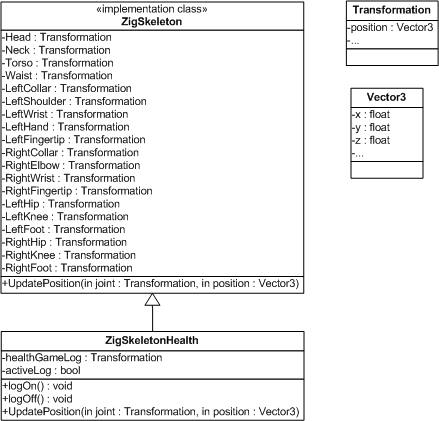
\includegraphics[scale=0.8]{./img/diagclasszigfu.png}
 \caption{Diagrama Classe ZigSkeleton e ZigSkeletonHealth}
 \label{fig:diagramaclassezigfu}
\end{figure}
%
%\begin{figure}[!htbp]
 %\centering
 %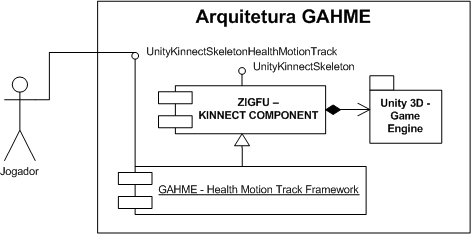
\includegraphics[scale=0.8]{./img/Unity3DArquitetura.png}
 %% matrixargseg.png: 296x162 pixel, 100dpi, 7.52x4.11 cm, bb=0 0 213 117
 %%\caption{Estágio desenvolvimento de jogos ~\cite{fullerton2008game}}
%\caption{Arquitetura do Jogo: Módulo Cliente de Captura de Dados}
%%  \caption{Estágio desenvolvimento de jogos}
 %\label{fig:arquitetura_cliente}
%\end{figure}

\subsubsection{Jogo: \textit{Catch the Spheres}}\label{jogo_catch}
Criamos o jogo \textit{Catch the Spheres} com a abordagem \textit{GAHME}. Seu desenvolvimento seguiu os Requisitos da Solução definidos na Seção~\ref{section:requisitos_solucao}.  

O \textit{Catch the Spheres} é em terceira pessoa e o jogador, por meio de seu personagem, deverá tocar ou desviar das bolas que vêm em sua direção. Se o jogador tocar as bolas azuis receberá uma pontuação por isso e caso seja atingido pelas bolas vermelhas  haverá uma penalização([REQ-GAHME-01]). Com o progresso do usuário as bolas tornam-se mais rápidas, exigindo uma maior agilidade nos movimentos ([REQ-GAHME-02]). Este é o principal mecanismo de fluxo do jogo que tem o intuito de atrair a atenção do jogador baseado nos desafios propostos ([REQ-GAHME-03]). 

Houve uma preocupação com a integridade física do jogador ([REQ-GAHME-04]), mas com numa análise com os usuários foi identificado que o mecanismo de desvio das bolas não é indicado para usuários com problemas de equilíbrio (Seção \ref{gqm_usuarios}) e este será removido em versões posteriores.

\begin{figure}[!htb]
     \centering
     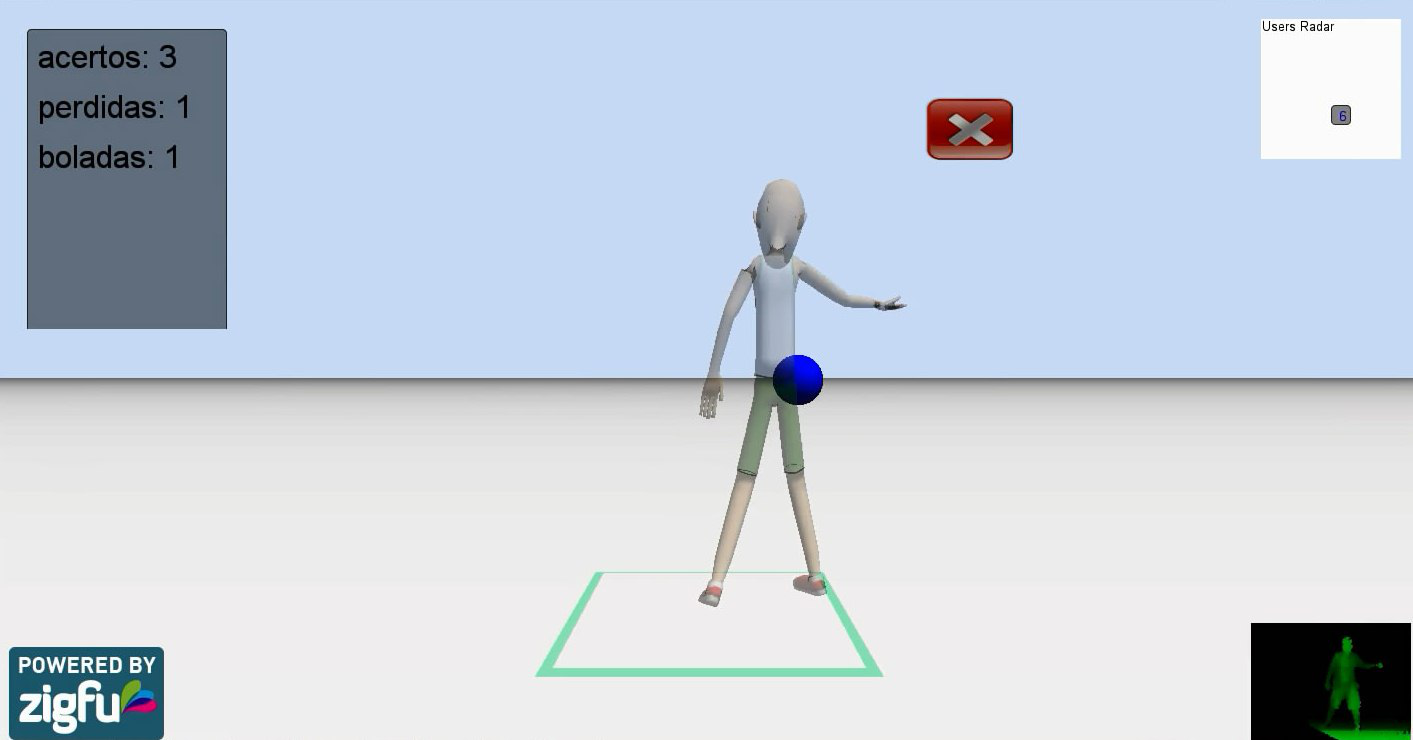
\includegraphics[width=.6\textwidth]{./img/catch-the-spheres.png}
     \caption{O jogo \emph{Catch the Spheres}}
     \label{img:catch}
\end{figure}

\subsection{Arquitetura do \textit{JOGUE-ME Webservice}}
O mecanismo de aquisição e armazenamento dos sinais motores ([REQ-GAHME-05]) torna possível a análise dos dados motores do usuário no qual o jogo armazena as informações e as envia para o servidor de dados. 

O \textit{GAHME Webservice} foi desenvolvido em colaboração com Antônio Santos Jr. em sua dissertação de mestrado ~\cite{antonio2013}. Do serviço de \textit{webservice} definido em seu trabalho (Figura~\ref{img:classd}), foram aproveitados os módulos de criação de usuário, recebimento de dados, gerenciador de arquivos e o módulo de escrita para gerar os arquivos a serem exportados e processados no MATLAB 2011 ~\cite{matlab2011} conforme a Arquitetura exposta na Figura~\ref{fig:arquitetura}.

\begin{figure}[!htb]
     \centering
     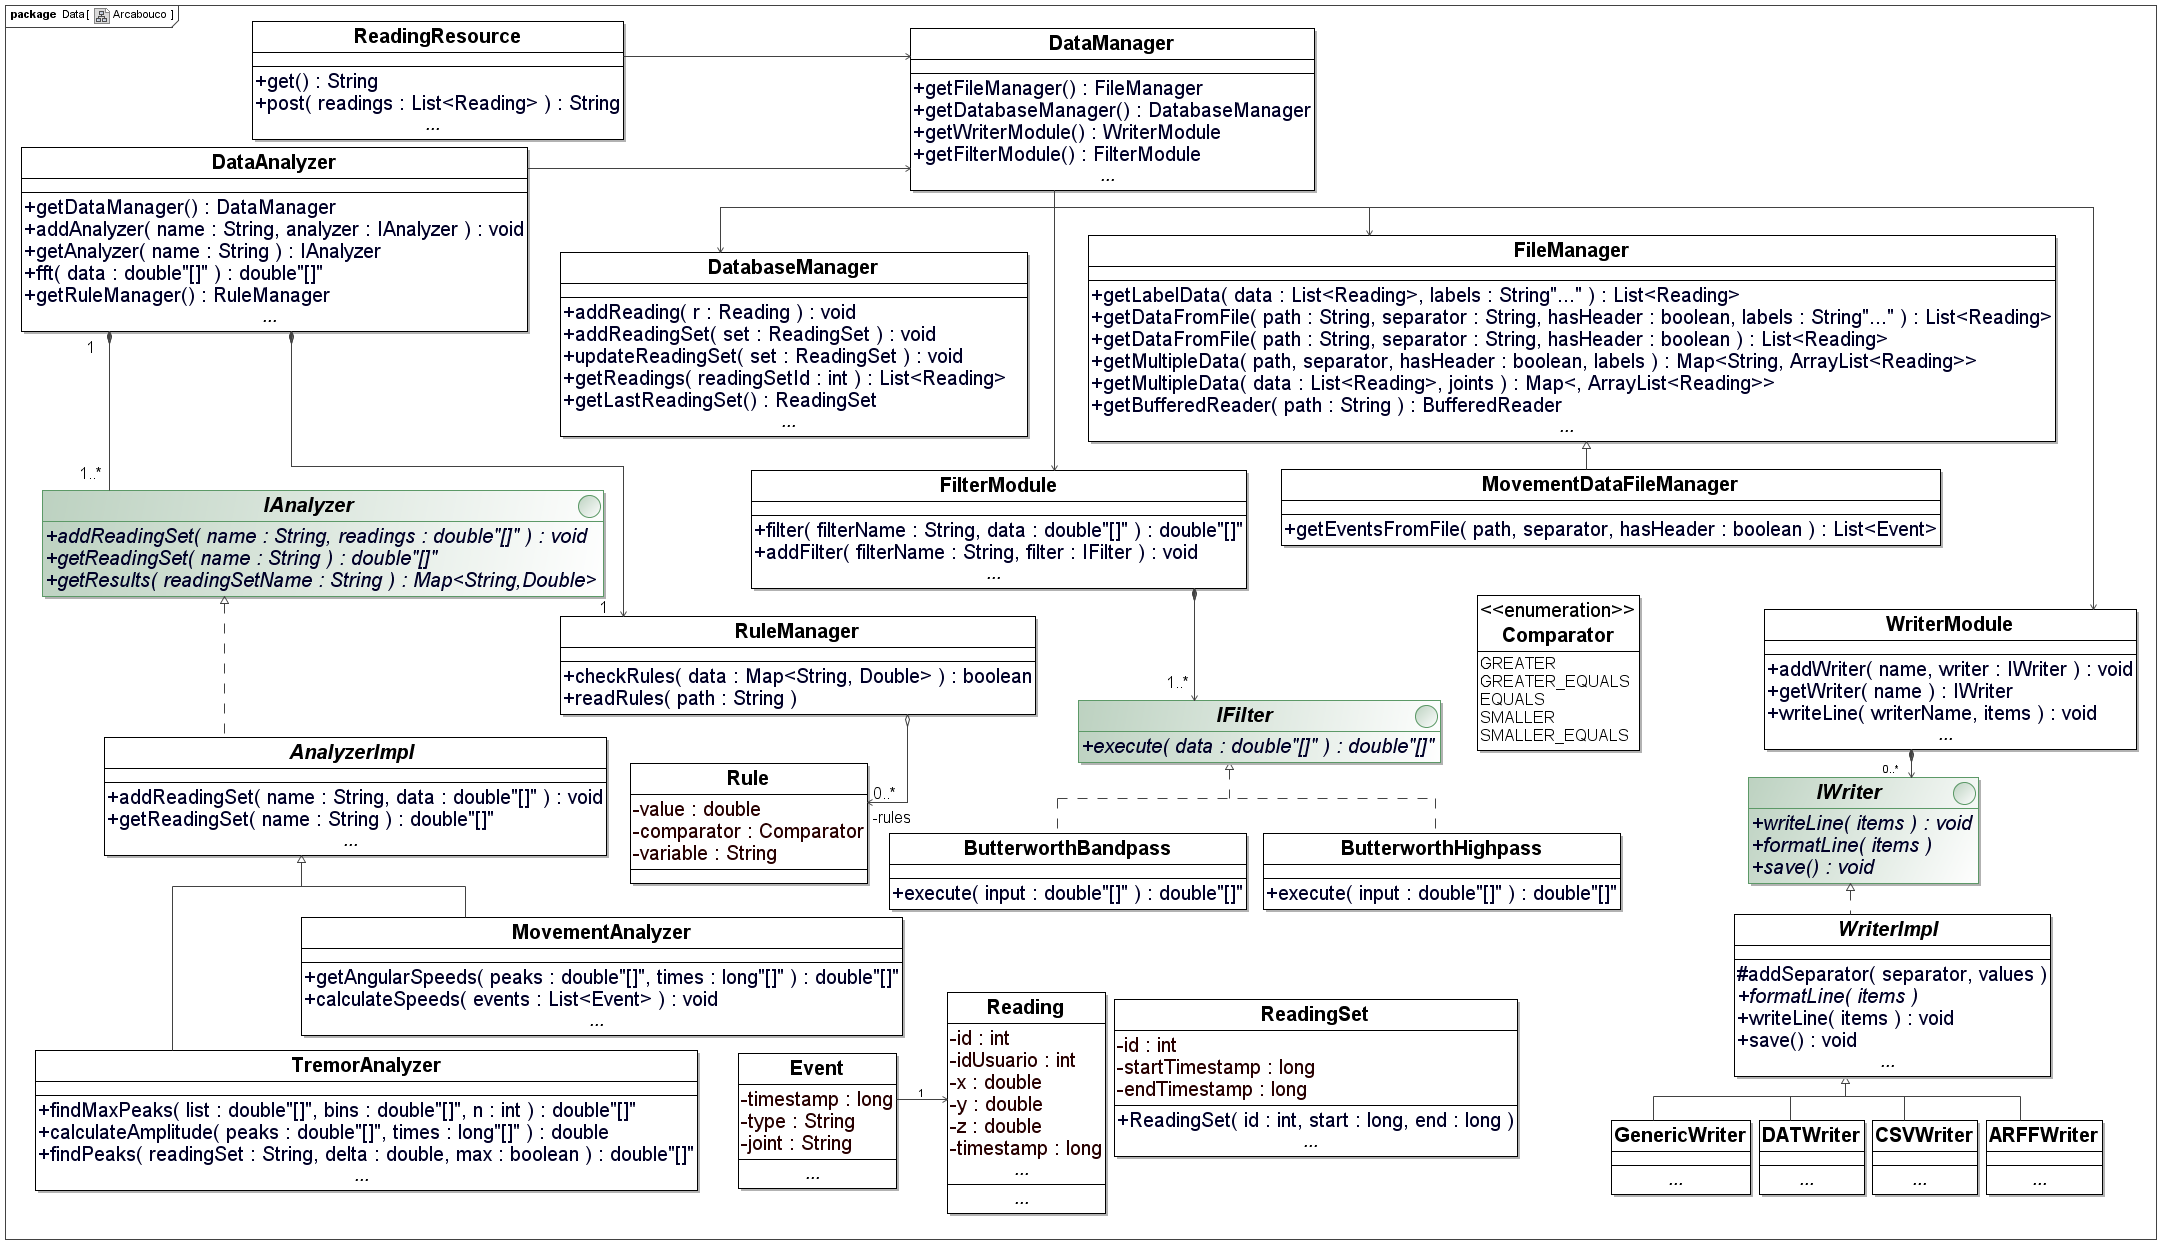
\includegraphics[width=1\textwidth]{./img/class_diagram.png}
     \caption[Diagrama de Classes do Arcabouço]{Diagrama de Classes do Arcabouço ~\cite{antonio2013}}
     \label{img:classd}
\end{figure}

O processo inicia com a aquisição dos dados dos sensores, que podem ser enviados para o \emph{webservice} e processados pela classe \texttt{ReadingResource} ou enviados por arquivos e processados pela classe \texttt{FileManager}, acessada através do \texttt{DataManager}. O \texttt{ReadingResource} envia os dados recebidos para o \texttt{DatabaseManager}, também acessado através do \texttt{DataManager}, para armazená-los no \emph{banco de dados} ~\cite{antonio2013}. Na Tabela~\ref{tab:operations}, ilustram-se as operações disponibilizadas pelo \textit{webservice} e um exemplo de como os dados devem ser estruturados para cada operação.

O envio dos dados dos usuários coletados com os dispositivos é feito através de uma requisição POST para o \textit{web service}. Os dados devem ser coletados durante uma sessão completa do jogo, que dura de alguns segundos a alguns minutos, para depois serem estruturados e enviados para o \textit{webservice}. O formato aceito pelas operações é o JSON (JavaScript Object Notation). 

\begin{table} 
\centering 
\caption{Operações disponibilizadas pelo \textit{web service}}
\begin{center}
    \begin{tabular}{ | l | c | l | }
        \hline
        Operação & Método & Exemplo \\ \hline
        cadastrarUsuario & POST & 
		\begin{minipage}{7cm}\begin{verbatim}
		
		{"id":2,"nome":"Ana",
		"masculino":false,
		"nascimento":"2012-11-28"}
		
		\end{verbatim}\end{minipage} \\ \hline
        obterToken & GET & - \\ \hline
        enviarDados & POST & 
		\begin{minipage}{7.5cm}\begin{verbatim}

		{"leitura":[{"id":0, 
		"idUsuario":1, "x":2.9097333, 
		"y":6.770132, "z":2.0355952, 
		"timestamp":1336134935706}, 
		{"id":0, "idUsuario":1, 
		"x":4.5565815, "y":4.9461093, 
		"z":1.4911331, 
		"timestamp":1336134935706}]}
		
		\end{verbatim}\end{minipage} \\ \hline
    \end{tabular}
\end{center}
\label{tab:operations}
\end{table}

\subsubsection{Gerenciador de Dados}
O \emph{Gerenciador de Dados} possui submódulos responsáveis por fazer leitura, separação e filtragem dos dados, além do gerenciamento destes no Banco de Dados com a escrita dos resultados disponibilizados pelo \emph{Analisador de Dados}. A classe \texttt{DataManager} implementa as funcionalidades do \emph{Gerenciador de Dados}, referenciando os quatro módulos: \emph{Gerenciador de Arquivos}, \emph{Módulo de Escrita}, \emph{Módulo de Filtragem} e \emph{Gerenciador do Banco de Dados}. Estes módulos serão explicados nas subseções a seguir. A classe \texttt{DataManager} possui um construtor \texttt{DataManager(DatabaseManager, FileManager, WriterModule, FilterModule)}, que recebe como parâmetros os quatro módulos. Dessa forma, é possível aumentar a funcionalidade de cada um dos módulos estendendo suas respectivas classes por herança e adicionando a elas novos métodos. A classe \texttt{MovementDataFileManager}, tratada mais adiante, é um exemplo de extensão do \texttt{FileManager}.

O \emph{webservice}, implementado utilizou a biblioteca Jersey\footnote{Disponível em: http://jersey.java.net/}, que facilita o desenvolvimento de \textit{RESTful webservices}. As requisições são enviadas para serem processadas pela classe \texttt{ReadingResource}, que é um \textit{web resource}, uma entidade que recebe requisições HTTP e envia respostas. Esta classe possui dois métodos, o \texttt{get()} que trata requisições \emph{GET}, retornando o identificador do último conjunto de leituras para controle do armazenamento no banco de dados; e o método \texttt{post(List<Reading> readings)} processa os dados das leituras enviados através de requisições \emph{POST}, e convertidos de JSON para objetos Java pela biblioteca Jersey. A classe \texttt{ReadingResource} está acoplada à classe \texttt{DataManager} e, através dela, tem acesso ao \emph{Gerenciador do Banco de Dados}. O \emph{webservice} pode ser instalado em qualquer \textit{web container}, como o Apache Tomcat\footnote{Disponível em: http://tomcat.apache.org/} e o GlassFish\footnote{Disponível em: http://glassfish.
java.net/}.

\subsubsection{Gerenciador de Arquivos}

A classe \texttt{FileManager} implementa o módulo \emph{Gerenciador de Arquivos}, que processa as operações de abertura de arquivos de dados delegadas pelo \emph{Gerenciador de Dados}. Esse módulo processa os dados recebidos, armazenando-os em dados estruturados para serem processado posteriormente pelo \emph{Analisador de Dados}. O dado estruturado aceito pelo \emph{Analisador de Dados} é composto por um rótulo identificador do dado, uma marca de tempo com precisão de milissegundos, e coordenadas x, y e z, cujo significado depende do tipo de sensor que as gera.

Os métodos da classe \texttt{FileManager} são:
\begin{enumerate}
	\item \texttt{getLabelData(List<Reading> data, String... labels)} filtra os dados da lista de leituras \texttt{data}, retornando uma nova lista \texttt{List<Reading>} contendo apenas os dados com os rótulos definidos em \texttt{labels}.
	\item \texttt{getDataFromFile(String path, String separator, boolean hasHeader)} lê os dados de um arquivo localizado no caminho \texttt{path}, cujos dados estão separados pelo separador \texttt{separator} e definidos linha a linha. O parâmetro \texttt{hasHeader} indica se o método deve procurar por uma linha de cabeçalho na primeira linha do arquivo. Retorna uma \texttt{List<Reading>} com os dados.
	\item \label{getdatamethod} \texttt{getDataFromFile(String path, String separator, boolean hasHeader, String... labels)} estende a funcionalidade do método anterior, retornando uma \texttt{List<Reading>} com os dados que possuem os rótulos definidos em \texttt{labels}.
	\item \texttt{getMultipleData(String path, String separator, boolean hasHeader, String... labels)} possui a mesma função que o método~\ref{getdatamethod}, mas, diferente deste, retorna um \texttt{Map<String, List<Reading>>} onde cada chave do mapa é um rótulo e indexa uma lista de eventos identificados pelo rótulo.
	\item \texttt{getBufferedReader(String path)} retorna um \texttt{BufferedReader} para manipular o arquivo cujo caminho é especificado dem \texttt{path}.
\end{enumerate}

A classe \texttt{MovementDataFileManager} estende as funcionalidades do \texttt{FileManager}, adicionando um método para leitura de eventos oriundos de jogos. Os eventos marcam o início ou fim de um momento específico do jogo no qual o jogador estará executando um movimento que será enviado para análise.

\subsection{Módulo de Escrita}

O \emph{Módulo de Escrita} é implementado pela classe \texttt{WriterModule}, que é responsável pela saída dos dados processados pelo \emph{Analisador de Dados}. Os dados podem ser estruturados para serem mostrados em um programa de plotagem de gráficos, como o GNUPlot\footnote{Disponível em: http://www.gnuplot.info/}, ou para servirem como entrada para mecanismos de aprendizado de máquina. Os dados são escritos em CSV (\textit{Comma-separated Values}) ou em qualquer outro formato definido pelo usuário do arcabouço. O módulo de escrita também suporta a escrita de arquivos ARFF, para serem processados pelo Weka\footnote{Disponível em: http://www.cs.waikato.ac.nz/ml/weka/}. O \emph{Módulo de Escrita} é extensível para permitir a geração de um formato de arquivo específico. A criação de um novo arquivo de dados é feita através da extensão da classe \texttt{WriterImpl} pela classe que se está criando.

A interface \texttt{IWriter} define três métodos para manipular arquivos de dados:

\begin{enumerate}
	\item \label{formatlinemethod} \texttt{formatLine(Object... items)} formata os itens \texttt{items} adicionando separadores ou qualquer outra formatação adicional definida na classe específica de escrita que implementa \texttt{IWriter} ou estende \texttt{WriterImpl}.
	\item \texttt{writeLine(Object... items)} escreve uma nova linha no arquivo, seguindo a formatação definida pelo método~\ref{formatlinemethod}.
	\item \texttt{save()} fecha a \textit{stream} de escrita dedicada ao arquivo e salva o arquivo em disco.
\end{enumerate}

A classe \texttt{WriterImpl} implementa os métodos comuns a todas as classes de escrita, definidos pela interface \texttt{IWriter}, fornecendo um método adicional para incluir separadores entre os elementos de uma linha. Para definir um comportamento diferente daquele implementado por \texttt{WriterImpl}, deve-se implementar diretamente a interface \texttt{IWriter}.

\section{Processador de Dados Biomecânicos}
O Processador de Dados Biomecânicos, foi implementado em MATLAB 2011~\cite{matlab2011} e como definido na ~\ref{sec:processador_bio} consiste de três passos: Identificação dos Ciclos, Extração de Características e Filtragem de Dados.

\subsection{Identificação dos Ciclos de Movimento} 
A identificação dos ciclos de movimento foi baseada na identificação de picos e vales do sinal motor como explicado na Seção~\ref{section:identificao_ciclos}. 

Para implementar o mecanismo de detecção de ciclos fez-se o uso da biblioteca \textit{Peak Detection in Matlab} ~\cite{peakdetect}. Essa biblioteca possui uma função chamada \textit{peakdet()} que recebe como parâmetros um vetor contendo o sinal a ser processado, e um valor de limiar para remoção do ruído do sinal. A função retorna dois vetores onde um possui os valores das máximas (picos) e o outro retorna os valores das mínimas (vales).

Usando a função \textit{peakdet()} criou-se a função \textit{cycleperiodic()} que tem o objetivo de identificar os ciclos periódicos de um sinal. Foram adicionados dois parâmetros a essa função para justamente levar em consideração o mínimo e o máximo a amplitude permitida do sinal.

\begin{lstlisting}[frame=single, caption=Função de Ciclo Periódico]  % Start your code-block

function [cycleIndex]=cycleperiodic(v, delta, maxAmplitude, minAmplitude)
[peaks, valey] = peakdet(v, delta);
j = 1;
for (i=1:(size(valey,1)-1))    
    initialIndex = valey(i,1);
    endIndex = valey(i+1,1);
    amplitude = endIndex - initialIndex;
    if ((maxAmplitude >= amplitude) & (minAmplitude <= amplitude))
        cycleIndex(j) = valey(i);
        j = j +1;
    end
end
\end{lstlisting}

De posse dos ciclos pode ser identificado quando começam e onde terminam os movimentos periódicos (Código Fonte~\ref{lst:identifyCycles}) como por exemplo os ciclos de marcha (Seção~\ref{section:analise_marcha} ou movimentos sucessivos de adução e abdução do braço (Seção ~\ref{fig:movabducaoaducao}). 

\begin{lstlisting}[frame=single, caption=Identificar Início e Tamanho do Movimento Periódico, label=lst:identifyCycles]  % Start your code-block

function [WindowBeginLeft, WindowLengthLeft, WindowBeginRight, WindowLengthRight] = identifyCycles(leftWristJoint, rightWristJoint)
    signalLeft = leftWristJoint(:,3);
    signalRight = rightWristJoint(:,3);

    cycleIndexLeft = cycleperiodic(signalLeft, 500, 200, 40);
    cycleIndexRight = cycleperiodic(signalRight, 500, 200, 40);

    WindowBeginLeft = cycleIndexLeft(1);
    WindowLengthLeft = cycleIndexLeft(size(cycleIndexLeft,2));
    WindowBeginRight = cycleIndexRight(1);
    WindowLengthRight = cycleIndexRight(size(cycleIndexRight,2));
\end{lstlisting}

\subsection{Extração das Características do Movimento}
Supondo que os ciclos de movimento foram identificados através da posição do punho, é necessário agora extrair as características do movimento. Para isso, o primeiro passo é calcular os ângulos relativos do movimento angular usando os pontos das articulações como pode ser visto no Código Fonte~\ref{lst:calculate_angle}. A função \textit{ArmRelativeAngleTorso()} realiza o cálculo do produto escalar entre as três articulações (Código Fonte:~\ref{code:produto_escalar}).

\begin{lstlisting}[frame=single, caption=Calcular ângulos relativos do movimento, label=lst:calculate_angle]
leftShoulderJoint = leftShoulderJoint(WindowBeginLeft:WindowLengthLeft,:);
leftWristJoint = leftWristJoint(WindowBeginLeft:WindowLengthLeft,:);  
leftHipJoint = leftHipJoint(WindowBeginLeft:WindowLengthLeft,:);  

for (j=1:size(leftHipJoint,1))
leftArmAngle(j,1) = leftHipJoint(j,1);
        

leftArmAngle(j,2) = ArmRelativeAngleTorso(leftHipJoint,leftShoulderJoint,leftWristJoint, j);    
end
\end{lstlisting}

De posse do sinal dos ângulos relativos do movimento, serão extraídos os picos e os vales desse sinal para  extrair a velocidade angular do movimento de abdução e adução do braço (Código Fonte: ~\ref{lst:angular_velocity}).
    
\begin{lstlisting}[frame=single, caption=Calcular Velociodade Angular Adução e Abdução, label=lst:angular_velocity]	
distanceup = cycle(peak) - cycle(1);
amplitude(identifiedCycles,1) = cycle(peak);
    
timestampupsec = (abs(timestampcycle(1) - timestampcycle(peak)))/1000;
velocityUp(identifiedCycles,1) = distanceup/timestampupsec;

distancedown = abs(cycle(end) - cycle(peak));
timestampdownsec = (abs(timestampcycle(peak) - timestampcycle(end)))/1000;
velocityDown(identifiedCycles,1) = distancedown/timestampdownsec;
\end{lstlisting}	
		
\subsection{Filtragem de Dados}
O filtro de dados tem o objetivo de remover os ciclos de movimento incompletos ou com problemas na aquisição dos dados, como explicado na Seção~\ref{section:filtro_dados}. Nessa etapa os ciclos são: normalizados, escalonados e rótulos do usuário (\textit{labels}). 
De posse de todos os dados é calculado um vetor médio dos ciclos normalizados para que seja possível definir um limiar (\textit{threshold}) de remoção dos ciclos (Código Fonte:~\ref{code:filtercycles}).

	\begin{lstlisting}[frame=single, caption=Calcular Velociodade Angular Adução e Abdução, label=code:filtercycles]
function [ KinnectData, processedCycles, labels ] = filterCyclesAndLabels (T, labels, otherFeatures, scaledLength)

    normalization = T;
    for i=1:size(T,1)
       normalization(i,1:scaledLength) = T(i,1:scaledLength)./max(T(i,1:scaledLength));
       normalization(i,scaledLength+1:scaledLength*2) = T(i,scaledLength+1:scaledLength*2)./max(T(i,scaledLength+1:scaledLength*2));
       normalization(isnan(normalization(i,1:scaledLength*2))) = min(normalization(i,1:scaledLength*2));
    end
    
    normalization(isnan(normalization)) = 0;
    
    if(size(T,2) > scaledLength*2) 
       normalization(:,scaledLength*2 + 1:end) =  T(:,scaledLength*2+1 : end)./max(T(:,scaledLength*2 + 1:end));
    end
    
    threshold = 1;
    meanOfNormalization = mean(normalization);
    u = ones(size(normalization,1),1);
    filterTestVector = sum((normalization - (u*meanOfNormalization)).^2,2);
    filterVector = filterTestVector<threshold;
    
       
    KinnectData = [T(filterVector,:) otherFeatures(filterVector,:)];
    processedCycles = T(filterVector,:);
    labels = labels(filterVector,:);    
end
\end{lstlisting}	


\section{Classificador de Dados}
Para avaliar os requisitos de identificação dos sintomas motores ([REQ-GAHME-06]) é necessário um teste com seres humanos para avaliar a aquisição e classificação dos sinais. A abordagem de classificação dos dados é baseada em máquinas de aprendizagem como explicado na Seção~\ref{section:class_dados}. O Código Fonte~\ref{code:classification} demonstra como fazer a classificação dos dados utilizando o \textit{Matlab Statistics Toolbox}~\cite{matlab2011}, o qual possui uma máquina de vetor de suporte disponível em sua biblioteca.

Primeiramente, separa-se o grupo de treinamento para realizar a aprendizagem da máquina utilizando o método \textit{svmtrain()}; depois utiliza-se o método \textit{svmclassify()} para predizer os valores usando a máquina de aprendizagem  e por fim calculam-se as diferenças entre os valores reais e os que foram classificados. Então, é calculada a taxa de erro para poder avaliar o resultado do classificador.

\begin{lstlisting}[frame=single, caption=Uso de Máquina de Vetor de Suporte para Classificação dos Dados, label=code:classification]
realValues; %Classe Atual
SVMStruct = svmtrain(trainingData,trainningClassification,'Kernel_Function', 'linear',	'BoxConstraint', 0.10);
class = svmclassify(SVMStruct, testData, 'showplot',true); %Classe Preditiva
classificationRate = sum(class~=realValues);
errorRate = classificationRate/size(classereal,2);
\end{lstlisting}
	
\chapter{Processo de Desenvolvimento de Jogos Eletrônicos Com Monitoramento de Dados de Saúde}\label{chap:processo_desenvolvimento}

Para a elaboração deste processo foi realizada uma revisão da literatura sobre processos de desenvolvimento de jogos tradicionais ~\cite{keith2010agile,moore2011basics,rucker2003software,kanode2009}, com o objetivo de identificar necessidades inerentes ao desenvolvimento de jogos voltados para saúde como pode ser visto em ~\cite{Suhonen_2010,herber2011,bartolome11,sinclair07,Hardy2011,kato12}. Este capítulo define um processo de desenvolvimento de jogos para entretenimento que permita o monitoramento de dados de saúde de modo não invasivo. 

%Para a elaboração desse processo foram utilizados estudos empíricos através de técnicas de pesquisa qualitativa com o uso de entrevista semi-estruturada \cite{FLI04} e observação participativa em um estudo de caso \cite{Yin05}. O resultado dessas avaliações estã descritos na \secref{section:analise_entrevista_semi_estruturada}. Como resultado dessa análise foram extraídos requisitos (\secref{section:requisitos_entrevista} e \secref{section:requisitos_estudo_caso}) que definiram algumas características e problemas de ambientes distribuídos de desenvolvimento, os quais requerem maior atenção em relação ao desenvolvimento presencial, como: uso de ferramentas colaborativas, meios de comunicação e coordenação das equipes distribuídas. 
O processo proposto, pode ser customizado posteriormente em outros contextos, desde quea equipe de desenvolvimento faça uma análise do processo e o instancie de acordo com suas necessidades.

A modelagem deste processo utiliza a semântica do meta-modelo \ac{spem} na Versão 2.0 \cite{spem08}, que permite modelar: métodos, atividades de processos de software através da notação gráfica UML. 

\section{Visão Geral}
O processo proposto chamado de \textit{GAHME Process}, tem como objetivo principal guiar o desenvolvimento de jogos eletrônicos com o objetivo monitorar dados de saúde (\textit{GAHME}). Desta maneira, pode-se dizer que a principal contribuição deste processo é fornecer um conjunto coerente de atividades e artefatos direcionados para o desenvolvimento de um \textit{GAHME}, mas que mantém a generalidade de um processo de desenvolvimento de \textit{software}, e pode ser aplicado no contexto de desenvolvimento de jogos.
%
%\begin{figure}
 %\centering
 %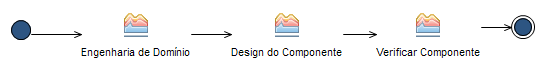
\includegraphics[scale=0.8]{./img/visaogeral.png}
 %% matrixargseg.png: 296x162 pixel, 100dpi, 7.52x4.11 cm, bb=0 0 213 117
 %%\caption{Estágio desenvolvimento de jogos ~\cite{fullerton2008game}}
%\caption{Visão Geral \textit{GAHME Process}}
%%  \caption{Estágio desenvolvimento de jogos}
 %\label{fig:visaogeral}
%\end{figure}
%
Atualmente, o \textit{GAHME Process} contempla duas fases distintas com responsabilidades definidas:
	%\begin{enumerate}
		%\item \textbf{Viabilidade:} A primeira fase deverá ser realizado um estudo sobre o público alvo, sintomas a serem monitorados, técnicas e tecnologias que permitam o monitoramento e a viabilidade de realizar o monitoramento dos dados de saúde por intermédio dos jogos eletrônicos.		
		%\item \textbf{Desenvolvimento:} A segunda fase utilizará os artefatos de software produzidos durante a primeira fase do processo para desenvolver um jogo eletrônico que permita realizar o monitoramento dos dados de saúde. No final da fase deverá ser realizada uma pesquisa com o público alvo do sistema para comprovar a eficácia do monitoramento.
	%\end{enumerate}
	
	\begin{enumerate}
	\item \textbf{Conceito:} responsável em definir o público alvo do jogo, identificar a população beneficiada, e avaliar o impacto do desenvolvimento do jogo. É de responsabilidade desta fase avaliar os sintomas monitoráveis bem como a existência de sensores capacitados. O término da fase será um estudo da viabilidade do monitoramento dos sintomas por meio dos jogos eletrônicos.
	\item \textbf{Pré-Produção:} definir as tecnologias utilizadas para o desenvolvimento do jogo, e testar a aquisição do sinal pelos sensores utilizando um protótipo desenvolvido. 
	Na Pré-Produção são elaborados cenários de jogos que permitam o monitoramento de dados, depois faz-se testes com os protótipos para a elaborar um artefato que define as ações monitoráveis dos jogadores (\textit{GAHME Action Design} Seção~\ref{subsec:game_actions_guide}).
\end{enumerate}

\section{Papéis e Responsabilidades}
A descrição dos papéis presentes no processo é importante para um melhor entendimento das atividades realizadas no processo. Nesta seção serão descritos os papéis previstos assim como suas principais habilidades e atribuições.


\subsection{\textit{Game Designer}}\label{subsec:game_designer}
O projeto de um jogo eletrônico é uma atividade multidisciplinar e requer a contribuição de diversos perfis e habilidades. O \textit{Game Designer} deve trabalhar em colaboração com todos os membros da equipe de desenvolvimento como Engenheiro de Software, \textit{Art Designer} e saber dos anseios do jogador ~\cite{schell2008art}. Um bom \textit{Game Designer} está disposto a escutar as diferentes opiniões e sugestões, para selecionar aquelas que melhorem a experiência do jogo ~\cite{moore2011basics}. Esse papel é responsável pela concepção, passando por atividades de: análise, melhorar o \textit{game design} e verificar o produto final.

\subsubsection{Habilidades}
Para desempenhar este papel é necessário que o integrante tenha as seguintes habilidades:
  \begin{itemize}
	  \item Entender dos anseios e ponto de vista do jogador em relação ao jogo ~\cite{schell2008art};
		\item compreender as ações monitoráveis do jogador definidos no \textit{GAHME Action Design} (Seção \ref{subsec:game_actions_guide});
		\item conceber o jogo o que confere narrativa, regras e objetivos~\cite{schell2008art,moore2011basics,bethke2003game}.
  \end{itemize}

\subsubsection{Abordagens de Atribuição}
O \textit{Game Designer} precisa conhecer as capacidades técnicas da equipe e das ações que monitoráveis do jogo, documentadas no \textit{GAHME Action Design}.

\subsection{\textit{Game Health Designer}}
O \textit{Game Health Designer} tem um papel bem parecido com o do \textit{Game Designer} (Seção \ref{subsec:game_designer}), mas com a responsabilidade de trabalhar em colaboração com o Profissional de Saúde e com o Engenheiro de Software para verificar a viabilidade do jogo. 

O \textit{Game Health Designer} elabora o \textit{GAHME Action Design} (Seção \ref{subsec:game_actions_guide}) que é o artefato que faz o mapeamento das ações monitoráveis e sua relação com os dados de saúde. 

\subsubsection{Habilidades}
Para desempenhar este papel é preciso:
  \begin{itemize}
	  \item Compreender as diretrizes médicas (Seção \ref{subsec:diretrizes_medicas});
		\item extrair sintomas monitoráveis com o auxílio do Profissional de Saúde;
		\item analisar as possibilidades de monitoramento por meio dos sensores disponíveis com o auxílio do Engenheiro de Software;
		\item verificar a viabilidade do monitoramento dos dados de saúde por meio de um jogo eletrônico;
		\item conceber um artefato de \textit{GAHME Action Design} que auxilie na concepção de um jogo.
  \end{itemize}

\subsubsection{Abordagens de Atribuição}
O \textit{Game Health Designer} deve ter conhecimento tanto da área de saúde quanto das tecnologias utilizadas no desenvolvimento dos jogos.

\subsection{Engenheiro de \textit{Software}}\label{subsec:engenheiro_software}
Esse papel é responsável por desenvolver o sistema. Os engenheiros de software utilizam como entrada o \textit{GAME Design} e o \textit{GAHME Action Guideline} gerado pelos \text{Designers}. É de extrema importância que esse perfil compreenda o \textit{GAME Design} para que o jogo desenvolvido esteja de acordo com sua especificação.

\subsubsection{Habilidades}
Para desempenhar este papel é preciso:

\begin{itemize}
    \item Definir e criar soluções técnicas através das tecnologias utilizadas no projeto.
		\item Comunicar e repassar a arquitetura da aplicação para os demais integrantes.
\end{itemize}

\subsubsection{Abordagens de Atribuição}
O perfil do engenheiro de software é mais técnico. Esse profissional deve dominar a tecnologia de desenvolvimento de jogos utilizada além de compreender da capacidade dos sensores utilizados no projeto.

\subsection{Profissional de Saúde}\label{subsec:profissional_saude}
O profissional de saúde representa o grupo interessado em receber os dados dos usuários, os quais serão monitorados. O compreendimento das necessidades e interesses desse profissional são elementos chave para o desenvolvimento de uma solução efetiva.

\subsubsection{Habilidades}
O papel de Profissional de Saúde detém o expertise da doença e dos sintomas monitorados.

\subsubsection{Abordagens de Atribuição}
O Profissional de Saúde, presente no processo de desenvolvimento, deve fornecer o conhecimento sobre os sintomas referentes a sua especialidade de formação. Auxiliando na compreensão dos sintomas e das ações dos usuários, que devem possibilitar o monitoramento.

Algumas doenças são acompanhadas por diferentes Profissionais de Saúde, sejam médicos e fisioterapeutas ou até mesmo médicos com diferentes especializações. Nestes casos, é necessário a participação dos diferente perfis de profissionais de saúde para que sejam colhidas informações com mais detalhes e possa envolver a opinião dos diferentes profissionais.




\section{Fase: Conceito}\label{sec:conceito}
A fase de Conceito tem como papéis principais para sua execução o \textit{Game Health Designer} e o \textit{Profissional de Saúde}. Estes perfis fazem a análise da viabilidade do monitoramento. Terminada essa atividade, o \textit{Game Designer} elabora cenários de jogos que permitem o monitoramento. Baseado nos cenários, o Engenheiro de \textit{Software} implementa protótipos de jogos para testar a abordagem. 

Por se tratar de um jogo voltado para o monitoramento da saúde, as diretrizes médicas possibilitará o suporte científico para interpretação dos dados. Podem ser analisados e reproduzidos os trabalhos científicos da área, para verificar a viabilidade de um jogo a ser desenvolvido.

\begin{figure}[!htb]
 \centering
 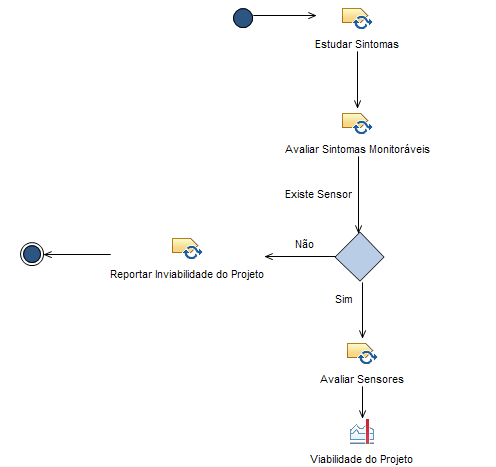
\includegraphics[scale=0.8]{./img/gahme-fase-conceito.png}
 % matrixargseg.png: 296x162 pixel, 100dpi, 7.52x4.11 cm, bb=0 0 213 117
 %\caption{Estágio desenvolvimento de jogos ~\cite{fullerton2008game}}
\caption{Fase de Conceito do \textit{GAHME Process}}
%  \caption{Estágio desenvolvimento de jogos}
 \label{fig:faseviabilidade}
\end{figure}


\subsection{Atividade: Identificar Público Alvo}
O \textit{Game Health Designer} define o perfil do jogador, essa é uma questão importante, pois define o público alvo do jogo. Isso ocasiona em avaliar a faixa etária a que se destina o jogo, pois jogos desenvolvidos para um público infantil tem um perfil bastante diferente dos voltados para adultos ~\cite{brathwaite2009challenges}. Por isso, o público alvo impacta diretamente na elaboração do \textit{Game Design} do projeto, pois o perfil do usuário pode necessitar de ambientes mais lúdicos em caso de crianças ~\cite{yannakakis06}, ou uma maior preocupação com situações de risco para caso o jogo seja direcionado para os idosos ~\cite{brox11,arntzen2011}.


\subsubsection{Papéis Responsáveis}
\begin{itemize}
	\item \textit{Game Health Designer};
	\item Profissional de Saúde.
\end{itemize}

\subsubsection{Passos para Execução da Atividade}
\begin{itemize}
	\item Avaliar faixa etária;
	\item avaliar necessidade de monitoramento;
	\item avaliar sintomas a serem monitorados.
\end{itemize}

\subsubsection{Artefatos de Entrada}
\begin{itemize}
	\item Diretrizes Médicas.
\end{itemize}

\subsubsection{Artefatos de Saída}
\begin{itemize}
	\item Seção de Análise de Impacto do documento de \textit{GAHME Design}.
\end{itemize}


\subsection{Atividade: Estudar Sintomas}
O objetivo principal dessa atividade é identificar sintomas monitoráveis usando as Diretrizes Médicas como base científica para a execução desta atividade e a opinião do Profissional de Saúde para melhor entendimento do sintoma e das práticas exercidas para a sua identificação. O \textit{Game Health Designer} faz um mapeamento dos sintomas e possíveis valores que identifiquem a sua ocorrência. 

O objetivo dessa atividade é identificar os sintomas monitoráveis sem levar em consideração a existência ou as especificações técnicas dos sensores que possibilite o monitoramento dos dados. 

\subsubsection{Papéis Responsáveis}
\begin{itemize}
	\item \textit{Game Health Designer};
	\item Profissional de Saúde.
\end{itemize}

\subsubsection{Passos para Execução da Atividade}
\begin{itemize}
	\item Identificar sintomas;
	\item avaliar necessidade de monitoramento dos sintomas;
	\item Descrever sintomas passíveis de monitoramento.
	%\item Especificar valores que identifiquem os sintomas;	
\end{itemize}

\subsubsection{Artefatos de Entrada}
\begin{itemize}
	\item Diretrizes Médicas.
\end{itemize}

\subsubsection{Artefatos de Saída}
\begin{itemize}
	\item Seção de Sintomas Passíveis de Monitoramento do documento de \textit{GAHME Design}.
\end{itemize}

\subsection{Avaliar Sintomas Monitoráveis}
Baseado na Seção de Sintomas Passíveis de Monitoramento do documento de \textit{GAHME Design} e na Especificação dos Sensores existentes o \textit{Game Health Designer} irá identificar e descrever quais são os sintomas monitoráveis. Para a elaboração deste artefato faz-se necessária a colaboração do Engenheiro de \textit{Software} por ter habilidades em tecnologia e este ser mais habilitado a compreender as especificação do sensor. O Profissional de Saúde tem papel auxiliar para esclarecer dúvidas sobre os sintomas e como o monitoramento deve ser efetuado.

O \textit{Game Health Designer} participa das discussões de saúde e tecnológicas, pois ele irá conceber quais serão as ações executadas pelo jogador, logo ele necessita entender tanto das limitações técnicas dos sensores quanto dos movimentos que o jogador efetua. 

%Para a execução desta atividade o \textit{Game Health Designer} deverá fazer uso do Documento de Diretrizes Médicas (Seção \ref{subsec:diretrizes_medicas}) para identificar a necessidade de monitoramento dos sintomas, juntamente com o Profissional de Saúde, deverão selecionar sintomas que identifique problemas de saúde e que sejam mensuráveis por intermédio de sensores. Durante a execução desta atividade também deve ser coletado as informações a respeito da importância, impactos e benefícios ao tratamento de saúde o público alvo terá ao ter esses sintomas monitorados.

\subsubsection{Papéis Responsáveis}
\begin{itemize}
	\item \textit{Game Health Designer};
	\item Engenheiro de \textit{Software};
	\item Profissional de Saúde.
\end{itemize}

\subsubsection{Passos para Execução da Atividade}
\begin{itemize}
	\item Analisar os sintomas monitoráveis;
	\item coletar sensores que possibilitem o monitoramento;
	\item estudar os principais sensores;
	\item mapear sintomas e sensores que possibilitem o monitoramento dos dados.
\end{itemize}

\subsubsection{Artefatos de Entrada}
\begin{itemize}
	\item Seção de Sintomas Monitoráveis do documento de \textit{GAHME Design}
\end{itemize}

\subsubsection{Artefatos de Saída}
\begin{itemize}
	\item Seção de Sintomas Monitorados do documento de \textit{GAHME Design}
\end{itemize}

%\subsection{Criar Arcabouço de \textit{Software} Para Captura de Dados}
%%Caso a equipe de desenvolvimento não tenha conhecimento ou experiência sobre uma \textit{engine} de jogos que atendam as necessidades do jogo para monitoramento de dados de saúde, 
%Essa atividade consiste em desenvolver um Arcabouço de \textit{Software}, que consiga adquirir dados dos sintomas passíveis de monitoramento conforme o \textit{GAHME Design}.
%
%O Engenheiro de \textit{Software} irá analisar as \textit{engine} de jogos existentes e os mecanismos que permitam integrar essa \textit{engine} com os sensores utilizados no jogo. Sensores como o acelerômetro do celular já possuem suporte nativo dentro das \textit{engine} de jogos para esses dispositivos ~\cite{unity3d}. Outros sensores como o MS-Kinnect ~\cite{kinnect2013} que é uma câmera que permite adquirir os movimentos do corpo, necessitam da instalação de \text{Device Drivers} e \textit{Componentes} de software a serem instalados dentro da \textit{engine} ~\cite{zigfu} para permitir a integração. Como referência a essa atividade podemos citar o trabalho de mestrado de Santos Jr.~\cite{antonio2013} que criou um arcabouço de software para monitoramento de dados de saúde com as tecnologias de acelerômetro presentes em celulares Android e do MS-Kinnect~\cite{kinnect2013}. 
%
%Nessa atividade também o Engenheiro de \textit{Software} pode identificar barreiras tecnológicas que inviabilizem o monitoramento dos sintomas. Nesse caso ele deve reportar a inviabilidade do projeto e terminar o ciclo de desenvolvimento. 
%
%\subsubsection{Papéis Responsáveis}
%\begin{itemize}
	%\item Engenheiro de \textit{Software};
%\end{itemize}
%
%\subsubsection{Passos para Execução da Atividade}
%\begin{itemize}
	%\item Analisar os sintomas passíveis de monitoramento;
	%\item coletar sensores que possibilitem o monitoramento dos sintomas;
	%\item estudar os principais sensores coletados;
	%\item mapear sintomas e sensores que possibilitem o monitoramento dos dados.
%\end{itemize}
%
%\subsubsection{Artefatos de Entrada}
%\begin{itemize}
	%\item Seção de Sintomas Passíveis de Monitoramento do documento de \textit{GAHME Design}
%\end{itemize}
%
%\subsubsection{Artefatos de Saída}
%\begin{itemize}
	%\item Arcabouço de \textit{Software} Para Captura de Dados..
%\end{itemize}

\subsection{Reportar Inviabilidade do Projeto}
A inviabilidade do projeto pode ter diferentes fatores, essa atividade ficará a cargo do Engenheiro de \textit{Software}, para a tomada de decisão, ele faz a captura dos sinais e verifica se o sensor tem a precisão necessária para identificar os sintomas. Caso o sensor ou as ações não sejam monitoráveis o Engenheiro de \textit{Software} elabora um documento justificando a inviabilidade do projeto.
%Existem casos que os sensores são capazes de adquirir os dados dos sintomas mas as ações dos usuários não podem ser utilizadas em um jogo eletrônico. Como por exemplo o sintoma de Tremor da ~\ac{dp} que é de repouso ~\cite{patel_monitoring_2009}. A \textit{priori}, não existe barreira tecnológica para identificar o sintoma de tremor usando os acelerômetros de um aparelho de celular e logicamente identificar o sintoma parkinsoniano. Mas, pacientes com essa patologia ao interagir com o dispositivo usando a mão, entram num estado ativo do membro cessando assim o tremor naquele momento inviabilizando o monitoramento e como consequência o projeto.

\subsubsection{Papéis Responsáveis}
\begin{itemize}
	\item Engenheiro de \textit{Software}.
\end{itemize}

\subsubsection{Papéis Auxiliares}
\begin{itemize}
	\item Profissional de Saúde.
\end{itemize}

\subsubsection{Passos para Execução da Atividade}
\begin{itemize}
	\item Analisar precisão dos sensores e comparar com os sintomas monitoráveis;
	\item explicar motivos que tornaram o monitoramento inviável.
\end{itemize}

\subsubsection{Artefatos de Entrada}
\begin{itemize}
	\item Seção de Sintomas Monitorados do documento de \textit{GAHME Design};
\end{itemize}

\subsubsection{Artefatos de Saída}
\begin{itemize}
	\item Seção de Inviabilidade de Monitoramento do documento de \textit{GAHME Design}
\end{itemize}



\section{Fase: Pré-Produção}
Os jogos para saúde precisam passar por pesquisa entre seres humanos e testado com grupo de controle para verificar sua eficácia~\cite{kato12}. Na pré-produção (Figura~\ref{fig:fasedesenvolvimento}), deve ser desenvolvido um protótipo do jogo para verificar sua viabilidade. Logo, se o protótipo desenvolvido for testado com seres humanos e os dados forem testados com uma boa eficácia finaliza-se a pré-produção. De posse dos artefatos deste processo, pode-se executar o ciclo de desenvolvimento de um jogo tradicional como definido em ~\cite{fullerton2008game}.

A fase de Pré-Produção tem como papéis principais para sua execução o \textit{Game Designer} e o Engenheiro de \textit{Software} e como resultado final a comprovação da eficácia do protótipo do jogo em relação ao monitoramento dos dados de saúde. 
\begin{figure}[!HTB]
 \centering
 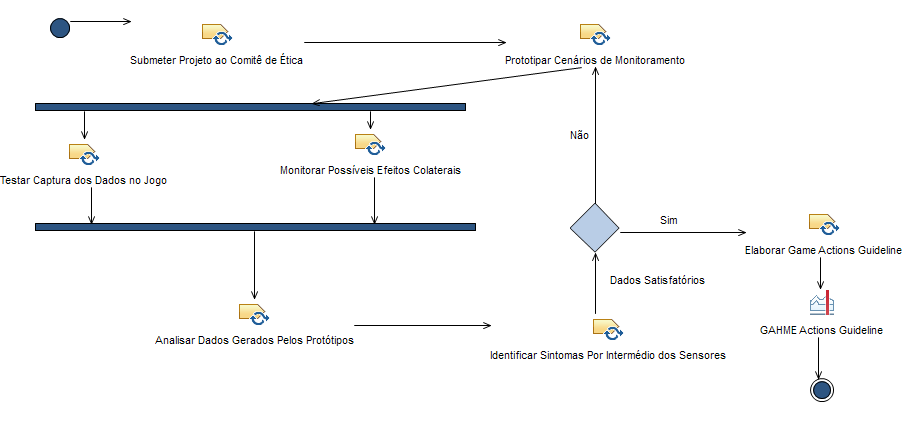
\includegraphics[scale=0.6]{./img/gahme-fase-pre-producao.png}
 % matrixargseg.png: 296x162 pixel, 100dpi, 7.52x4.11 cm, bb=0 0 213 117
 %\caption{Estágio desenvolvimento de jogos ~\cite{fullerton2008game}}
\caption{Fase de Pré-Produção do \textit{GAHME Process}}
%  \caption{Estágio desenvolvimento de jogos}
 \label{fig:fasedesenvolvimento}
\end{figure}
\FloatBarrier



%Nos últimos anos houve um crescimento de jogos voltados para saúde, contudo muito desses jogos não foram validados efetivamente ou foi realizado um estudo para verificar os seus resultados ~\cite{kato12}. Os estudos realizados por muitos desses jogos foram mal projetados e suas conclusões não podem se consideradas válidas ou eficazes. Por esse motivo Kato ~\cite{kato12} sugeriu diretrizes para a realização de estudos de eficácia para ser aplicados em jogos para saúde. 
%Como a iteração de "Verificação" é responsável por avaliar a eficácia do monitoramento dos dados de saúde a partir do jogo desenvolvido, as sugestões definidas por Kato ~\cite{kato12} estarão presentes no decorrer da iteração.






%

%
%\begin{enumerate}
	%\item \textbf{Desenvolvimento:} A iteração de implementação será bem semelhante a uma fase de produção de um jogo tradicional ~\cite{fullerton2008game}, tendo como produto final da fase o jogo desenvolvido. Contudo, o \textit{Game Design} deverá levar em consideração as ações do jogador que permitem monitoramento (\textit{GAHME Actions Guideline}). No término desta fase, o jogo deverá ser testado com o objetivo de identificar se os mecanismos de captura de dados de saúde do jogo foram desenvolvidos corretamente.
	%\item \textbf{Verificação:} 	O desenvolvimento de um jogo por si só é uma tarefa multidisciplinar ~\cite{fullerton2008game} e esta quando aplicada num contexto de saúde necessita de mecanismos para verificar a eficácia da abordagem adotada ~\cite{kato12}. Nessa fase, a proposta do jogo deverá ser submetida para a avaliação do conselho de ética médica, para que possa ser testado com seres humanos e verificar se os sintomas monitorados foram corretamente identificados.
%\end{enumerate}

\subsection{Submeter Projeto ao Comitê de Ética}
O objetivo dessa atividade é submeter o protótipo do jogo às normas regulamentadoras previstas para a pesquisa envolvendo seres humanos segundo a Resolução 196/96 ~\cite{conselho2000normas}. Segundo o Conselho Nacional de Saúde ~\cite{conep2002}, o ~\ac{cep} é um colegiado interdisciplinar e independente,  que deve existir nas instituições que realizam pesquisas envolvendo seres humanos no Brasil, criado para defender os interesses dos sujeitos da pesquisa em sua integridade e dignidade e para contribuir no desenvolvimento da pesquisa dentro de padrões éticos (Normas e Diretrizes Regulamentadoras da Pesquisa Envolvendo Seres Humanos - Res. CNS 196/96 ~\cite{conselho2000normas}). 

O \ac{cep} é responsável pela avaliação e acompanhamento dos aspectos éticos de todas as pesquisas envolvendo seres humanos. Este papel está bem estabelecido nas diversas diretrizes éticas internacionais (Declaração de Helsinque, Diretrizes Internacionais para as Pesquisas Biomédicas envolvendo Seres Humanos – CIOMS) e Brasileiras (Res. CNS 196/96 e complementares~\cite{conselho2000normas}), diretrizes estas que ressaltam a necessidade de revisão ética e científica das pesquisas envolvendo seres humanos, visando a salvaguardar a dignidade, os direitos, a segurança e o bem-estar do sujeito da pesquisa ~\cite{conep2002}.
%
%Nessa atividade deve ser elaborado um Protocolo de Pesquisa, contemplando a descrição da pesquisa, estabelecer critérios de inclusão e exclusão dos sujeitos da pesquisa, a qualificação dos pesquisadores e todas instâncias responsáveis pelo projeto. Estão presentes no projeto Instituições de pesquisa, legitimamente constituída e habilitada que permita realizar as investigações científicas. 

Os pesquisadores elegem os riscos da pesquisa, principalmente danos físicos, psíquicos, moral, intelectual, cultural do ser humano em qualquer fase de uma pesquisa dela decorrente ~\cite{conselho2000normas}. Sendo necessária a anuência do sujeito da pesquisa ou de um representante por intermédio do Consentimento livre e esclarecido, onde será explicado a natureza da pesquisa, seus objetivos, métodos, benefícios previstos, potenciais riscos e o incômodo que esta possa acarretar, formulada em um termo de consentimento, autorizando sua participação voluntária na pesquisa ~\cite{conselho2000normas}. Caso o sujeito da pesquisa se enquadre nos critérios estabelecidos para interromper a pesquisa, essa deverá ser finalizada assegurando a integridade do mesmo. Como o Profissional de Saúde possui em sua formação a natureza da pesquisa além de conhecer os métodos que serão aplicados durante a pesquisa ele possui o perfil mais habilitado para desempenhar essa atividade.


Atualmente no Brasil para poder testar o jogo com monitoramento de dados de saúde junto a pacientes, e consequentemente testar sua eficácia, é necessário passar por esse processo e obter a aprovação de um \ac{cep}. Este é um processo demorado e pode impactar a entrega final.

\subsubsection{Papéis Responsáveis}
\begin{itemize}
	\item Profissional de Saúde.
\end{itemize}

\subsubsection{Passos para Execução da Atividade}
\begin{itemize}
	\item Analisar os sintomas a serem monitorados;
	\item Identificar objetivo da pesquisa;
	\item Identificar potenciais riscos e estabelecer critérios para interromper a pesquisa;
	\item Identificar benefícios previstos.
\end{itemize}

\subsubsection{Artefatos de Entrada}
\begin{itemize}
	\item Diretrizes Médicas;
	\item Seção de Sintomas Monitorados do documento de \textit{GAHME Design}.
\end{itemize}

\subsubsection{Artefatos de Saída}
\begin{itemize}
	\item Projeto Submetido ao Comitê de Ética Médica;
	\item Termo de Consentimento Livre e Esclarecido.
\end{itemize}

%\subsection{Identificar Sintomas Por Intermédio dos Sensores}
%Baseado nos

 

%\subsection{Monitorar Possíveis Efeitos Colaterais}
%Durante a execução da pesquisa possíveis efeitos colaterais devem ser monitorados como: risco de queda, fadiga, tendinite. 
%As avaliações de jogos para a saúde devem tentar controlar o uso de seu jogo para efeitos colaterais negativos, outro possível efeitos colateral negativo dos jogos é a ocorrência de convulsões, devido à fotossensibilidade.








\subsection{Verificar Eficácia do Jogo}
A eficácia do jogo será verificada através de um estudo analítico de caso-controle ~\cite{menezes2001epidemiologia}, dentro de um ambiente aprovado pelo \ac{cep} que permitirá recrutar sujeitos de pesquisa. Uns sujeitos deverão apresentar os sintomas a serem monitorados e outros não terão tais sintomas. Os dados serão coletados e ao final deverá ser verificado se os sintomas foram corretamente identificados.

Kato ~\cite{kato12} defende que para essa verificação é necessário obter um número adequado de participantes para conseguir avaliar o impacto do jogo. Contudo, determinados sintomas possuem poucos sujeitos de pesquisa disponíveis reduzindo a abrangência da pesquisa.

%Em uma revisão sistemática sobre a eficácia dos jogos existes e que promovem a atividade física para adolescentes ~\cite{foley-active-game2010}, segundo a revisão a abordagem de jogos se mostrou eficaz ao motivar a execução de atividade física dos usuários. Os jogos estudaram envolveram tanto os membros superiores quanto inferiores do corpo melhorando a atividade de forma prazerosa e com qualidade inclusive em grupos de deficiência e de alto risco.

%Verificar essa referencia ~\cite{Primack2012630}

%\subsection{Atividade: Publicar Resultados}


\subsection{Atividade: Elaborar \textit{GAHME Design}}
De posse dos movimentos e da captura dos dados descritos no \textit{Game Action Guideline}. ´É elaborado um \textit{game design} inclui os movimentos no contexto do jogo eletrônico ~\cite{sweetser2005-gameflow}, este jogo possui mecanismos de monitoramento dos dados de saúde embutidos. Para a execução desta atividade, leva-se em consideração um processo iterativo, que precisa é: protipar, testar e refinar continuamente até concluir~\cite{brathwaite2009challenges}.



%\section{Iteração: Prototipação}
%O objetivo desta iteração é desenvolver um protótipo que permita capturar dados de saúde e ao término desta iteração deverá ser elaborado o \textit{GAHME Actions Guideline} (Seção \ref{subsec:game_actions_guide}) que conterá as ações executadas pelo jogador que possam ser monitoráveis e que venham a ser utilizadas pelo \textit{Game Designer} durante a fase de Desenvolvimento. 
%
%Alinhar a jogabilidade e a possibilidade de monitoramento frequente dos dados de saúde não é uma tarefa trivial. Pois deve ser levado em consideração o uso dos dispositivos e pensar na execução de movimentos ou ações que permitam esse monitoramento. Para propor um jogo com monitoramento de dados de saúde deve ser realizado um estudo sobre quais os movimentos e ações que o usuário deve executar. De posse dessas ações, deve ser desenvolvidos protótipos que permitam testar a execução dessas atividades e capturar os dados com o objetivo de estudar mecanismos que permitam identificar esses sintomas conforme os trabalhos já existentes e que possuem tal propósito ~\cite{Ballegaard:2008:HEL:1357054.1357336,albanese2012,bachlin_wearable_2010,visionbased2009,patel_monitoring_2009}. 
%
%\begin{figure}
 %\centering
 %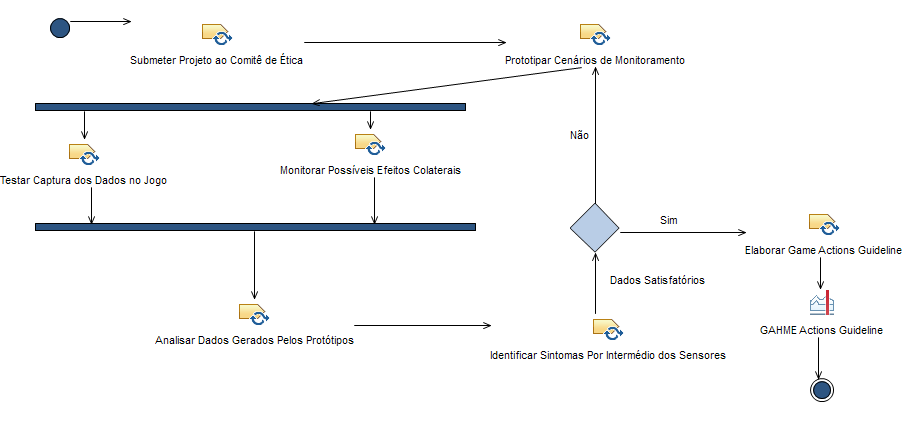
\includegraphics[scale=0.55]{./img/gahme-fase-pre-producao.png}
 %% matrixargseg.png: 296x162 pixel, 100dpi, 7.52x4.11 cm, bb=0 0 213 117
 %%\caption{Estágio desenvolvimento de jogos ~\cite{fullerton2008game}}
%\caption{Iteração: Prototipação do \textit{GAHME Process}}
%%  \caption{Estágio desenvolvimento de jogos}
 %\label{fig:prototipaccao}
%\end{figure}


%Os movimentos não podem ser repetitivos pois, levaria o usuário jogar por um curto período e como consequência abandonaria o monitoramento ~\cite{Suhonen:2008:SFE:1457199.1457204}. 



 

%\subsection{Engenheiro de Software}
%Esse papel é responsável por desenvolver o sistema. Os engenheiros de
%software devem utilizar como entrada o \useacronym{DER} gerado pelos engenheiros de requisitos. É
%de extrema importância que os engenheiros de software entendam o
%\useacronym{DER} para que o produto desenvolvido esteja de acordo com sua
%especificação.
%
%\textbf{Habilidades}
%
%Para desempenhar este papel é necessário que o integrante tenha o
%perfil com as  seguintes habilidades:
%
%\begin{compactenum}
    %\item Definir e criar soluções técnicas através das tecnologias utilizadas no projeto.
    %\item Identificar e construir casos de teste que venham cobrir o
%comportamento requerido pelos componentes do sistema.
    %\item Comunicar e repassar a arquitetura da aplicação para os
    %demais integrantes.
%\end{compactenum}
%
%\textbf{Abordagens de Atribuição}
%Mesmo em equipes pequenas, os indivíduos devem trabalhar em grupo no
%desenvolvimento de soluções técnicas.
%
%Cada integrante pode executar tarefas especificas de acordo com suas
%habilidades, porém é desejável que as demais tecnologias utilizadas
%no projeto sejam do conhecimento de todos, para que haja uma maior
%troca de auxilio técnico entre os integrantes.




\section{Artefatos}

%Os documentos para o desenvolvimento de jogos tem dois propósitos principais: histórico do projeto e comunicação ~\cite{schell2008art}. O desenvolvimento de um jogo requer a tomada de decisões a todo o momento, que definem o funcionamento do jogo. Contudo, existe uma grande probabilidade de que os envolvidos do projeto não se recordem dos motivos que as decisões foram tomadas. Se a equipe de desenvolvimento tiver o hábito de armazenar todas as tomadas de decisões e documentá-las nos artefatos utilizados no desenvolvimento do software então não será necessário rediscutir as decisões já tomadas ~\cite{schell2008art}.
Os artefatos de software servem como documentos de entrada e saída da execução de atividades dentro do próprio processo ~\cite{sommerville2011}.

\subsection{Diretrizes Médicas}\label{subsec:diretrizes_medicas}
O principal propósito da atividade médica é o cuidado com o paciente, e isso traz enormes desafios de forma coletiva ou individual. Com o intuito de auxiliar na tomada de decisões, a comunidade médica mundial tem elaborado e divulgado um extenso número de informações ~\cite{nhs2013,neozeland-guide-2013}, muito mais acessíveis do que era no passado, redefinindo o universo do conhecimento médico, tornando-o livre e acessível para críticas e demais propósitos científicos ~\cite{proj-diretriz2013}.

%Neste contexto, a Associação Médica Brasileira e o Conselho Federal de Medicina, com o objetivo de auxiliar na tomada de decisão médica e, consequentemente, otimizar o cuidado aos pacientes, desencadearam um processo junto às Sociedades de Especialidade para a elaboração de Diretrizes Médicas baseadas nas evidências científicas disponíveis na atualidade ~\cite{proj-diretriz2013}.
%
%Nesse processo, formou-se uma Comissão Técnica responsável em construir as bases de sustentação das recomendações de conduta médica, utilizando os meios da ciência atual, de forma crítica e desprovida de interesse se não aquele que resulte na melhoria do tratamento do médico com o paciente. 

Partindo do princípio que o conhecimento médico atual está presente nas diretrizes médicas e que através do seu conteúdo é possível extrair informações que permitam: identificar, avaliar a presença e evolução de sintomas de doenças. 
%Nas diretrizes médicas estão descritos mecanismos de diagnósticos, prognóstico, tratamento, dosagem medicamentosa, riscos e benefícios. Além de definir questões mais relacionadas à prática clínica e descrevendo as possíveis opções para a tomada de decisão sobre o tratamento da doença .a ser monitorada como por exemplo a Doença de Parkinson que servirá como estudo de caso do presente trabalho ~\cite{protpar010}.
%evidências através dos dados sobre a doença bem como mecanismos de diagnósticos, prognóstico, tratamento, dosagem medicamentosa, riscos e benefícios. Além de definir questões mais relacionadas à prática clínica e descrevendo as possíveis opções para a tomada de decisão sobre o tratamento da doença .a ser monitorada como por exemplo a Doença de Parkinson que servirá como estudo de caso do presente trabalho ~\cite{protpar010}.
\subsubsection{Propósito}
As diretrizes médicas permitem identificar sintomas monitoráveis, bem como parâmetros relevantes a esses sintomas. Este documento é escrito pela comunidade médica e é considerado como base científica sobre o tema abordado. Para o \textit{GAHME Process} este artefato servirá de artefato de entrada para fundamentar quais sintomas serão monitorados e de que forma serão avaliados.


%\subsection{Estudos Epidemiológicos}\label{subsec:estudos_epidemiologicos}
%A Epidemiologia é a ciência que estuda ocorrência de doenças em populações humanas e seus fatores determinantes das doenças ou condições relacionadas à saúde em populações especificadas no estudo ~\cite{menezes2001epidemiologia,lima-costa-2003}. Inicialmente a epidemiologia restringia-se a estudo de epidemias de doenças transmissíveis, contudo atualmente a epidemiologia trata qualquer evento relacionado à saúde (ou doença) da população ~\cite{menezes2001epidemiologia}.
%
%%\subsubsection{Tipos de Estudos epidemiológicos}
%Os estudos epidemiológicos podem ser classificados em observacionais e experimentais, para o este trabalho serão utilizados estudos epidemiológicos observacionais descritivos têm por objetivo determinar a distribuição de doenças ou condições relacionadas à saúde, segundo o tempo, o lugar e/ou as características dos indivíduos ~\cite{lima-costa-2003}. Ou seja, responder à pergunta: quando, onde e quem adoece? Logo, as respostas dessas perguntas serão fundamentais para avaliar o impacto de possíveis tratamentos, medicamentos trabalho ou em nosso caso do desenvolvimento de um jogo que permita o monitoramento de dados de saúde.
%
%A epidemiologia descritiva pode fazer uso de dados secundários (dados pré-existentes de mortalidade e hospitalizações, por exemplo) e primários (dados coletados para o desenvolvimento do estudo) ~\cite{lima-costa-2003}. No Brasil, existem importantes bancos de dados secundários com abrangência nacional que podem ser usados para estudo epidemiológicos como: Sistema de Informações sobre Mortalidade (SIM-SUS) ~\cite{sis2013}, Pesquisa Nacional de Amostra Domiciliar (PNAD) ~\cite{pnad2008} bem como os estudos epidemiológicos realizados no Brasil e disponibilizados em Bases de estudo em saúde como Scielo ~\cite{scielo2013}.

%\subsubsection{Propósito}
%O propósito deste artefato é identificar a população beneficiada como o monitoramento dos dados de saúde por intermédio dos jogos eletrônicos.


\subsection{\textit{GAHME Action Design}}\label{subsec:game_actions_guide}
\subsubsection{Documento de Sintomas Monitoráveis}
Esse artefato é o princial artefato da fase de \textit{Concepção}, é através dele que será decidida a viabilidade do desenvolvimento do jogo nas fases seguintes do processo de desenvolvimento. Contudo, mesmo sendo um artefato elaborado na primeira fase do processo de desenvolvimento, este não será descartado nas demais fases pois deverá ser testado e refinado nas fases seguintes do processo.


\subsubsection{Cenário de Jogo}
A fase de conceito do cenário do jogo para muito autores é definida como crucial para conseguir um jogo de sucesso e atingir elementos difíceis de ser mensurados como por exemplo a diversão. O uso de protótipos nas etapas iniciais do processo de desenvolvimento permitem anteceder o comportamento do jogo e auxiliar na definição do mesmo durante a elaboração do \textit{Game Design}, pois os jogadores podem experimentar o jogo nas etapas iniciais e permite que estes teçam suas opiniões~\cite{prototipgames2007}.
 
Para conceber os cenários iniciais, não precisa necessariamente desenvolver um jogo. Estudos indicam que mecanismos de prototipagem rápida ou de baixo custo ~\cite{prototipgames2007,fullerton2008game} permitem o entendimento da ideia proposta e habilita aos participantes a discussões logo no início do projeto, reduzindo o custo com modificações em fases mais adiantadas do desenvolvimento. 

%Fullerton ~\cite{fullerton2008game}, defende que a prototipação física permite que os participante se concentrem nos mecanismos do jogo sem se preocupar com os aspectos tecnológicos do mesmo, possibilitando que membros da equipe que não tem perfil técnico possam mostrar sua perspectiva e consequentemente contribuir no \textit{game design}. 


%Como pode ser visto na Figura \ref{fig:proto-fps}um exemplo de protótipo físico de um cenário de jogo de um FPS, essa abordagem permite a compreensão sobre a estratégia do jogo, visualização de possíveis cenários e até mesmo a alteração do mesmo de forma rápida, contrastando com a dificuldade de alterar um ambiente 3D digital ~\cite{fullerton2008game}. 

%\begin{figure}
 %\centering
 %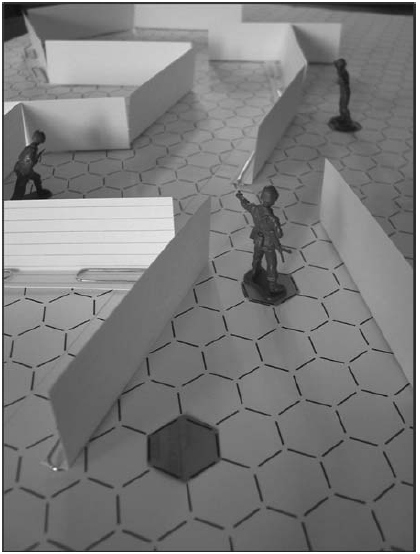
\includegraphics[scale=0.55]{./img/fps-fisical-prototype.png}
 %% matrixargseg.png: 296x162 pixel, 100dpi, 7.52x4.11 cm, bb=0 0 213 117
 %%\caption{Estágio desenvolvimento de jogos ~\cite{fullerton2008game}}
%\caption{Prototipação Física de um \ac{fps} ~\cite{fullerton2008game}}
%%  \caption{Estágio desenvolvimento de jogos}
 %\label{fig:proto-fps}
%\end{figure}

%Uma das etapas do planejamento do designer passa pela concretização da suas ideias através de modelos que consigam certificar de que a concepção é realmente divertida e através de protótipos será possível demonstrá-la para os demais membros da equipe, garantindo que será dada continuidade ao projeto para a produção definitiva ~\cite{prototipgames2007}. Os benefícios do uso de protótipos rápidos é que ele permite testes rápidos de componentes separadamente sem necessariamente implementar o sistema completo como também encoraja usuários a comentar livremente e sugerir modificações (contrário a um produto bem acabado que pode parecer já terminado). Porém, como ponto negativo, temos muitas vezes componentes individuais devem ser re-testados no produto finalizado ~\cite{prototipgames2007}.


%
%
%
%
%\subsection{Protótipo Jogável}
%Game prototypes, while playable, usually include only a rough approximation of the artwork, sound, and features. They are very much like sketches whose purpose is to allow you to focus on a small set of the game’s ~\cite{fullerton2008game}. There are many types of prototypes, including physical prototypes, visual prototypes, video prototypes, software prototypes, etc. 
%
%Prototyping lies at the heart of good game design. Prototyping is the creation of a working model of your idea that allows you to test its feasibility and make improvements to it ~\cite{fullerton2008game}. 
%
%%Buskirk e Moroney [2003] afirmam que o uso da técnica de prototipagem pode ser estendido para outras fases do ciclo de vida do produto além dos testes de usabilidade. Sendo usado na validação dos requisitos junto aos consumidores, na fase de especificação do projeto, desenvolvimento dos manuais do produto, suporte ao marketing, execução de testes funcionais, ajuda no serviço de atendimento aos clientes ~\cite{prototipgames2007}.O público-alvo dessa avaliação inicial inclui publishers, engenheiros de software, artistas, e outros membros da equipe. Como “palavras são fundamentalmente uma maneira terrível de comunicar interatividade” [Waugh 2006], podemos tomar o desenvolvimento de protótipos como meio para ajudar a educar a equipe de como alguns componentes do jogo deveriam se comportar, esclarecendo de forma mais amigável os conceitos abstratos e poder transmitir como o jogo deve funcionar ~\cite{prototipgames2007}.
%If you try to design the entire game at once, you might become confused and overwhelmed. There are so many elements in a typical game that it is diffi cult to know where and how to start. What we recommend is that you isolate the core gameplay mechanisms and build out from there ~\cite{fullerton2008game}.
%
%
%
%\subsection{GAHME Actions Guideline}\label{subsec:game_actions_guide}
%
%Para elaboração deste artefato o \textit{Game Health Designer}, utilizará como irá utilizar as Diretrizes Médicas como base científica de conhecimento e das especificações dos sensores de captura que poderão ser utilizados.
%
%Para elaboração deste artefato o 
%
%Para a sua elaboração o responsável Os artefatos de entrada para elaboração
%
%O responsável pela elaboração do GAHME Actions Design é o que deverá se basear nas Diretrizes Médicas, para fazer uma avaliação dos mPara elaboração do GAHME Actions Design, o autor 
%
%Nesse artefato é levado em consideração o sensor utilizado, o sintoma a ser monitorado e a eficácia do monitoramento sendo comprovada por intermédio de testes efetuados na atividade \textit{Testar Protótipos} da fase de \textit{Prototipação}.
%
%The core gameplay mechanism, or “coremechanic,” can be defi ned as the actions that a player repeats most o en while striving to achieve the game’s overall goal. Games are repetitive by nature. While the meaning and consequences of what a player does can change over the course of game, the core actions tend to remain the same from beginning to end ~\cite{fullerton2008game}.
%
%Creating a physical prototype is a critical step in the design of your original game concept. It will save your team tremendous amounts of time because everyone will have a clear understanding of the game you are making. In addition, a physical prototype will enable you to focus your creative energy on the game mechanics without becoming distracted by the production and programming process ~\cite{fullerton2008game}. 
%
%
%
%\subsection{GAHME Actions Design}
%O objetivo deste artefato é definir quais são os movimentos efetuados pelo jogador dentro do jogo que são passíveis de monitoramento. Para elaboração deste artefato o \textit{GAHME Designer}, irá utilizar as Diretrizes Médicas como base científica de conhecimento e das especificações dos sensores de captura que poderão ser utilizados.
%
%Por promover atividades físicas, ou ações que possam trazer injúria ao jogador, como movimentos de equilíbrio, movimentos repetitivos ou rápidos. O game design do jogo deve ter a preocupação de desenvolver o jogo de acordo com o público-alvo. Isso significa dizer que a faixa etária e limitações físicas e cognitivas em decorrência da idade ou enfermidade devem ser levadas em consideração. Os jogadores devem ter a segurança de usarem o jogo e ter a certeza que o seu uso não acarretará em injúria ~\cite{arntzen2011}.
%
%
%
%
%
%Para elaboração deste artefato o 
%
%Para a sua elaboração o responsável Os artefatos de entrada para elaboração
%
%O responsável pela elaboração do GAHME Actions Design é o que deverá se basear nas Diretrizes Médicas, para fazer uma avaliação dos mPara elaboração do GAHME Actions Design, o autor 
%
%Nesse artefato é levado em consideração o sensor utilizado, o sintoma a ser monitorado e a eficácia do monitoramento sendo comprovada por intermédio de testes efetuados na atividade \textit{Testar Protótipos} da fase de \textit{Prototipação}.
%


%\input{Processo de Desenvolvimento}
%\input{Arquitetura da Solucao}
%\chapter{Identificação de Padrões da Análise de Movimento}\label{sec:analise_movimento_identificacao_padroes}
%O reconhecimento dos padrões de movimento de Parkinsonianos é bastante importante para o diagnóstico da \ac{dp}. Entretanto, existem poucos métodos  que identificam esses padrões específicos da doença. 



%O que é ..
%Para que serve
%Como funciona9
%Importância para Identificação de Padrões


\section{}
%Para a avaliação dos resultados do trabalho é necessário  realizar os testes juntamente com Pacientes de Parkinson e Voluntários como grupo de controle. A presente pesquisa teve o projeto aprovado junto ao conselho de ética médica aprovado pelo Comitê de Ética em Pesquisa (CAAE: 14408213.9.1001.5182) e os pacientes foram informados sobre os procedimentos e assinaram um termo de consentimento livre e esclarecido. 
%Contudo, o número de voluntários é insuficiente para testar a abordagem com máquinas de aprendizagem (11 voluntários, 5 pacientes com AVC e 6 diagnosticados com Doença de Parkinson). Por esse motivo recorremos a base de dados da Physionet para avaliarmos o presente trabalho e consequentemente aumentarmos nosso espaço amostral.




%\subsection{Avaliação dos Resultados}
%Para a avaliação dos resultados do trabalho é necessário  realizar os testes juntamente com Pacientes de Parkinson e Voluntários como grupo de controle, no momento esta sendo aguardado o parecer de ética médica.
%Contudo, foi a abordagem de processamento de sinal, reconhecimento de padrões e classificação usando SVM a ser usada no trabalho está sendo testada com a base de dados de paciente de Parkinson da Physionet. Essa base de dados contêm a\ac{fvrs}, capturada através de 8 sensores em cada pé.
%Uma etapa importante para a aprendizagem de máquina é a seleção dos dados. Baseados nas diretrizes médicas dos sintomas parkinsonianos,  como entrada para a SVM foram processados os ciclos de movimento e para cada ciclo foram calculados: 
%A média da VGRF: Informará se existe muita mudança na força do movimento como consequência alteração no equilíbrio
%SwingPhase/Stance Phase (Figura 2.) e a diferença da média da força do pé esquerdo sobre o pé direito, o parkinsoniano tem um passo mais curto logo a Fase de Balanço será mais curta.
%Diferença da força do pé da esquerda sobre o da direita: A partir da fase 2 da \ac{dp} existe uma assimetria do movimento logo o parkinsoniano demonstraria essa diferença.




\chapter{Avalia\c{c}\~{a}o Experimental} \label{chap:avaliacao}
Neste capítulo são descritos os experimentos realizados para a validação deste trabalho.

A realização do monitoramento dos sinais motores de uma maneira não-invasiva é um desafio, logo esta tese fornece uma forma lúdica de monitorar os dados de saúde por meio de jogos eletrônicos que podem ser integrados à rotina diária dos usuários. %Pois, a partir de um \textit{HGMS-E} é possível capturar, processar e classificar os movimentos cinéticos exercidos pelos usuários.

%Sabendo que o acompanhamento de sinais motores, integrados à rotina diária do paciente traz benefícios ao tratamento e qualidade de vida do mesmo do ponto de vista do profissional da saúde. Por intermédio desse trabalho, conseguimos capturar dados motores utilizando sensores de movimento. Esses dados permitem auxiliar no acompanhamento de doenças com comprometimento motor tal como o~\ac{dp}. Então, neste trabalho nós desenvolvemos um mecanismo de de captura de dados motores embutidos num jogo eletrônico, o qual permite monitorar e quantificar os sinais motores de uma forma lúdica e não-invasiva.




\section{ETAPA 1 - Entrevista Semiestruturada com Profissionais de Saúde}\label{chapter:entrevista_semi_estruturada}

A interpretação de dados é o cerne da pesquisa qualitativa, esse método tem como função desenvolver a teoria, servindo ao mesmo tempo de base para a decisão sobre quais dados adicionais devem ser coletados, por meio de codificação seletiva~\cite{FLI04}. Esta técnica, permite elaborar uma categorização nos dados, demonstrando ao pesquisador quais são os fenômenos mais preponderantes da pesquisa. O procedimento da interpretação dos dados, assim como a integração de material adicional são encerrados quando se atinge a "saturação teórica", ou seja quando o avanço na codificação não resulta na aquisição de novos conhecimentos~\cite{FLI04}.

Para análise dos textos provenientes da pesquisa foram transcritos as entrevistas com: neurologistas e fisioterapeutas especialistas em neurologia. Com  a codificação seletiva foi possível categorizar os as ocorrências de acordo com o conteúdo de cada texto. Ou seja, as respostas de cada participante foram analisadas incluídas na árvore de categorias como sugere o método de pesquisa~\cite{FLI04}. 

Para auxiliar no processo de: análise, seleção e codificação. Foi utilizado uma ferramenta de suporte à pesquisa qualitativa (\textit{QDA Miner}~\cite{qda13}), por meio desta, foi possível categorizar e reformular a árvore de categorias~\cite{FLI04} diversas vezes durante o processo de análise~\cite{FLI04}.


\subsection{Objetivo da Pesquisa}
O objetivo da entrevista semiestruturada~\cite{FLI04} foi entender como é feito o acompanhamento do paciente com sintomatologia do~\ac{dp}, juntamente aos profissionais de saúde: neurologistas que prescrevem a dosagem medicamentosa e fisioterapeutas que fazem o tratamento  de reabilitação e acompanhamento motor do paciente. Esse profissionais de saúde, foram indagados se haveria melhora na tomada de decisão caso estes pudessem acompanhar os sinais motores em diariamente. Procurou-se encontrar dentro do contexto de estudo, a importância do monitoramento de dados de saúde e os benefícios trazidos por este.

As entrevistas foram realizadas presencialmente, com perguntas não estruturadas e, com uma maior estruturação no decorrer da entrevista preocupando-se em evitar a referência do entrevistador sobre os pontos de vista do entrevistado, conforme sugere o método científico~\cite{FLI04}. 

\subsubsection{Instrumento de Análise dos Dados da Pesquisa Qualitativa} \label{section:analise_dados} 
A pesquisa qualitativa assistida por computador permite uma melhor categorização das informações obtidas em modo texto. O \textit{software} QDA Miner~\cite{qda13} auxilia o pesquisador na organização dos registros da pesquisa e das interpretações dos mesmos, justificando-se o uso da ferramenta devido a dificuldade de classificar e analisar os dados obtidos. Nessa análise, foram consideradas as atividades referentes ao acompanhamento dos sinais motores em pacientes com~\ac{dp}. Buscou-se durante a pesquisa avaliar se um cenário de monitoramento dos sinais motores por meio de jogos eletrônicos auxiliaria os profissionais de saúde quanto ao tratamento de seus pacientes.

Nesta seção, faz-se um detalhamento do resultado da entrevista semiestruturada, descrevendo a opinião dos entrevistados e coletando requisitos baseado nas necessidades expostas pelos mesmos. Por meio desta etapa da pesquisa foi avaliada a \textbf{ETAPA 1} da pesquisa: \textit{Quais os benefícios de acompanhar diariamente os sinais motores do paciente do ponto de vista do profissional da saúde}.

%	\begin{description}

%	\item[H1] O acompanhamento de sinais motores integrados à rotina diária do paciente, traz benefícios ao tratamento e na qualidade de vida do mesmo, do ponto de vista do profissional da saúde.
% 	\end{description}
	
%\subsubsection{Análise da Entrevista Semi-Estruturada}
%A análise qualitativa ~\cite{FLI04} permite identificar as práticas dos profissionais de saúde referentes ao acompanhamento dos sinais motores em pacientes de parkinson e como essas práticas podem ser aperfeiçoadas num cenário em que haja o monitoramento dos sinais. 


\subsection{Perfil dos Participantes}
O perfil dos participantes é composto por quatro profissionais da saúde, dos quais: dois são fisioterapeutas com especialização em neurologia, e dois são médicos neurologistas. A escolha desse perfil se fez de acordo com seus ofícios e responsabilidades e complementaridade quanto ao tratamento do paciente. Os neurologistas realizam o diagnóstico e acompanham os sinais motores juntamente com as informações obtidas do paciente ou de seu cuidador, e baseado nas informações realiza o gerenciamento da dosagem medicamentosa da doença. Por outro lado, os fisioterapeutas fazem o acompanhamento dos sinais motores em sessões de fisioterapia promovendo a aprendizagem motora desses pacientes. Logo, esses profissionais possuem visões e preocupações distintas e inerentes a seu ofício. 

Para manter a confidencialidade de informação, os entrevistados receberam uma \textbf{LEGENDA} que identifica o perfil profissional seguido por um número sequencial, o qual identifica o entrevistado mas preserva sua identidade (Tabela~\ref{table:perfil_analise_participantes}).

\begin{table}[h]
\caption{Perfil dos Participantes}
\label{table:perfil_analise_participantes}
\begin{tabular}{|l|l|c|c|}
\hline
\textbf{LEGENDA} & \textbf{PROFISSÃO}             & \multicolumn{1}{|l}{\textbf{IDADE (ANOS)}} & \multicolumn{1}{|l|}{\textbf{EXPERIÊNCIA (ANOS)}} \\ \hline
FIS\_01          & Fisioterapia em Neurologia & 40                                         & 10                                                \\ \hline
FIS\_02          & Fisioterapia em Neurologia     & 39                                         & 10                                                \\ \hline
NEU\_01          & Médico Neurologista            & 42                                         & 15                                                \\ \hline
NEU\_02          & Médico Neurologista            & 67                                         & 30                                                \\ \hline
\end{tabular}

\end{table}

\subsubsection{Questionário de Pesquisa}
Para a formulação do questionário foram realizadas análises nas diretrizes médicas ~\cite{protpar010,national2006parkinson} e na tabela UPDRS ~\cite{updrs87} sobre o progresso da ~\ac{dp} e dos sinais monitoráveis por sensores de movimento. Para a entrevista foram elaboradas 15 perguntas agrupadas em 3 seções (Apêndice \ref{apendice:entrevista-semi-estruturada}) com os seguintes temas: sinais do~\ac{dp}, monitoramento da saúde motora e os benefícios advindos do monitoramento. Onde o entrevistador selecionou as questões de acordo com o perfil profissional.

\subsection{Análise}
Durante a análise das entrevistas foram extraídos fragmentos, e a nomenclatura utilizada contém o prefixo \textbf{FRAGMENTO} mais um número sequencial identificando o mesmo. Esse procedimento permite identificar \textbf{requisitos} que orientem a proposta de monitoramento de dados motores por intermédio de jogos eletrônicos. Logo, os requisitos extraídos nesta abordagem foram obtidos a partir da perspectiva do profissional de saúde em relação ao tratamento e acompanhamento da~\ac{dp}. 

\subsubsection{Diagnóstico}\label{section:analise_diagnostico}

Na entrevista junto aos neurologistas, foi indagado como o diagnostico da~\ac{dp} é realizado.  A entrevista corroborou com a literatura médica~\cite{tolosa06,vedolin2003} em relação ao diagnóstico de exclusão do \ac{dp}~\cite{protpar010,national2006parkinson}.  

Todos os profissionais informaram que o sintoma mais comum é o tremor de repouso, e que este inicialmente é unilateral e seguido de uma bradicinesia como podemos perceber nos ([FRAGMENTO-01][FRAGMENTO-02]). Ainda no ([FRAGMENTO-01]), existe uma ocorrência do \textbf{[NEU\_01]} em que o mesmo evoca sobre a importância da técnica de \textit{Finger Taps} ~\cite{updrs87} para avaliação da bradicinesia.


\begin{quote}
\textbf{[FRAGMENTO-01][NEU\_01]} - 
\emph{
O diagnóstico da doença de Parkinson é quando o paciente chega se queixando de tremor. Esse sintoma começa com um tremor unilateral geralmente pelas mãos, lentamente progressivo e de repouso. Além do tremor esse paciente exibe também uma lentidão que a gente consegue detectar pelo \textit{Finger Taps}. Essa técnica consiste em tocar o polegar ao primeiro e segundo dedo simultaneamente para ver se há ou não lentidão. Faz-se uma comparação sempre com o outro lado para visualizar possíveis diferenças. 
Existe também uma rigidez no braço, quando faz-se uma flexão e extensão do membro e percebe-se que o tônus desse paciente comparado com o outro lado exibe uma diferença.
}
\end{quote}

\begin{quote}
\textbf{[FRAGMENTO-02][NEU\_02]} -
\emph{
O diagnóstico da doença de Parkinson é feito com uma das queixa iniciais do paciente é um tremor de repouso, geralmente associado a uma dificuldade na marcha. Então normalmente os pacientes reclamam de uma perna presa e um tremor de repouso. 
}
\end{quote}

Uma ocorrência no ([FRAGMENTO-03]) que deve ser ressaltado, é o que o entrevistado referiu como ``\textit{boa resposta ao prolopa}''. Essa ocorrência é denominada de diagnóstico diferencial da \ac{dp} ~\cite{protpar010}, consiste na redução dos sinais parkinsonianos em decorrência da resposta ao tratamento medicamentoso. 

\begin{quote}
\textbf{[FRAGMENTO-03][NEU\_01]} - 
\emph{
Então os sinais é o tremor em repouso, a lentidão e a rigidez. Inicialmente apenas de um lado, por exemplo começa no braço direito e depois vai para a perna direita, depois para o braço esquerdo e depois a perna esquerda. Isso lentamente progressivo, a gente faz a exclusão com outras doenças através de outros exames como tomografia, ressonância ou a uma boa resposta ao prolopa.
}
\end{quote}

\subsubsection{Sintomas}
Nesta seção estão expostos sinais para o acompanhamento da sintomatologia da ~\ac{dp}.

%\subsubsection{Tremor}
O sintoma de tremor, além de ter sido referenciado durante o diagnóstico da doença na Seção ~\ref{section:analise_diagnostico} por todos os entrevistados, possui particularidades como a dificuldade de controlar o sintoma por intermédio do tratamento medicamentoso ([FRAGMENTO-04]), e não é tão incapacitante quanto a bradicinesia ~\ac{dp}. No ([FRAGMENTO-05]) o [NEU\_01] reforçou sobre a importância de controlar os sinais de lentidão do movimento ante os de tremor ~\cite{do2007parkinson}.

\begin{quote}
\textbf{[FRAGMENTO-04][NEU\_01]} - 
\emph{
Mas a gente tem que ver, porque as vezes o tremor é muito mais difícil de você controlar. Porque está relacionada ao emocional do paciente. Quanto mais emocionalmente desequilibrado o paciente tiver, mais tremor ele tem.
}
\end{quote}

\begin{quote}
\textbf{[FRAGMENTO-05][NEU\_01]} - 
\emph{
O controle do tremor é um pouco complicado porque é um sintoma mais difícil de ser controlado com as medicações que temos hoje.  Então você poderia ver nesse seu projeto a lentidão. Porque o paciente quer tremer mas ele não quer ficar lento.
}
\end{quote}


%\subsubsection{Bradicinesia}\label{section:analise_bradicinesia}

O pesquisador indagou se o sintoma da bradicinesia era considerado o mais debilitante da ~\ac{dp} e como resposta ele obteve a afirmação de que a bradicinesia impacta diretamente na qualidade de vida do paciente, privando-o de realizar atividades diárias ([FRAGMENTO-06]).

\begin{quote}
\textbf{[FRAGMENTO-06][NEU\_01]} - 
\emph{
É ele atrapalha né, principalmente no levantar no andar, para você se levantar, pentear o cabelo o tremor é prejudicial. Porém mais prejudicial ainda é a lentidão do movimento.
}
\end{quote}

Ao indagar se o movimento de adução e abdução do braço seria relevante para a identificação da~\ac{dp}, o [NEU\_01] informou que a bradicinesia é um sintoma que traz lentidão em todo o corpo e possivelmente seria afetada por este movimento. Pois, devido à redução dos movimentos automáticos ([FRAGMENTO-07]), traz outros impactos físicos ao paciente ([FRAGMENTO-08]).

\begin{quote}
\textbf{[FRAGMENTO-07][NEU\_01]} - 
\emph{
Na verdade o movimento em si, vai ver o quão lento está. Porque você não tem um déficit motor. O comprometimento na doença de Parkinson está no comprometimento piramidal, o comprometimento extra-piramidal não vai estar alterando a força motora. O que vai estar vai ser exatamente a lentidão. Por exemplo, é um paciente que está andando você que os movimentos dele automáticos estão reduzidos, principalmente no balançar dos braços. Você vai andando, vai andando, você vê aquele paciente que está com a força, ele está com toda a estrutura piramidal tudo normal. Mas ela anda lento em consequência da lentidão do movimento porque os movimentos automáticos estão reduzidos.
}
\end{quote}


\begin{quote}
\textbf{[FRAGMENTO-08][FIS\_01]} - 
\emph{
Os sinais mais frequentes a gente tem a bradicinesia que é a lentificação do movimento, a gente tem um padrão postural que começa a ficar bem nítido que o paciente apresentar o Parkinson. Você percebe uma perda da movimentação automática da cintura escapular e aí ele começa a apresentar uma diminuição no volume da voz que é uma diplofonia, e apresenta uma maior rigidez muscular. Eles reclamam bastante e a bradicinesia que tornam os movimentos cada vez mais lentos.
}
\end{quote}

%\subsubsection{Marcha}
% Foi identificada uma ocorrência na dificuldade do andar do paciente de~\ac{dp}, quando o [NEU\_01] cita no ([FRAGMENTO-07]) (``\textit{Você vai andando, vai andando, você vê aquele paciente que está com a força, ele está com toda a estrutura piramidal tudo normal. Mas ela anda lento em consequência da lentidão do movimento ...}''. O [NEU\_02] corrobora com a mesma opinião ao citar a dificuldade de iniciar a marcha no ([FRAGMENTO-09]). O fisioterapeuta no papel de realizar o acompanhamento da marcha nas sessões fisioterápicas, fornece um aprendizado motor para a melhora da qualidade de vida do paciente de acordo com suas limitações ([FRAGMENTO-10]).
% 
% \begin{quote}
% \textbf{[FRAGMENTO-09][NEU\_02]} - 
% \emph{
% Problema na marcha. Dificuldade de iniciar a marcha, certa dificuldade de um lado comprometido. Mesmo quando o sintoma está unilateral eles sentem dificuldade para iniciar a marcha.
% }
% \end{quote}
% 
% \begin{quote}
% \textbf{[FRAGMENTO-10][FIS\_01]} - 
% \emph{
% Numa marcha, o doente de Parkinson tem a tendência de estar olhando para o chão. Mas a gente sabe que isso não é compatível com uma boa marcha a tendência é cair, para piorar eles têm os passos miúdos e também um passo arrastado. Então esse passo favorece a queda, poise ele perdeu a marcha automática que é aquela que a gente adquire na infância. O que a gente faz nas sessões de fisioterapia é tentar aplicar auto-correções para adaptar o paciente à nova realidade para que ele tenha uma aprendizado motor e no futuro um automatismo do movimento.
% }
% \end{quote}
% 
% Devido a quantidade de ocorrências sobre a análise da marcha para o acompanhamento da ~\ac{dp}, e a possibilidade da ocorrência de quedas dos indivíduos. Esses, dois fatos corroboraram com o uso de base de dados contendo dados sobre a marcha, pois isto vai além do custo financeiro para a aquisição dos sensores que capturam a ~\ac{fvrs}. Logo, ao usar bases contendo esses dados para a pesquisa, preserva-se a integridade física dos pacientes.



\subsubsection{Monitoramento Motor}
Nesta seção está exposta a importância do monitoramento dos sinais capturados no estudo analítico de caso controle definido no método de pesquisa na Seção~\ref{section:estudo_caso_controle}. Nesse estudo também pretende-se identificar as características dos movimentos que possam ser extraídos desses sinais, e que venham fornecer subsídios para diferenciar indivíduos diagnosticados com~\ac{dp} ante indivíduos sem o diagnóstico.

%\subsubsection{Amplitude do Movimento dos Braços}

Ao indagar ao [FIS\_02] se o movimento de adução e abdução do braço seria relevante para a identificação da~\ac{dp}, este informou que mesmo não sendo um teste específico para a identificação da doença, existem diferenças significativas encontradas em indivíduos diagnosticados com parkinson [FRAGMENTO-11].
\begin{quote}
\textbf{[FRAGMENTO-11][FIS\_02]}-
\emph{
Sim. Existe alterações sim, mas eu nunca vi especificamente esse teste como sendo usado para diagnóstico da doença. Mas que realmente existem mudanças no movimento de adução e abdução de uma pessoa normal ante a um parkinsoniano.
}
\end{quote}

O [FIS\_01], explicou os motivos que levam a perda da mobilidade no movimento de adução e abdução ([FRAGMENTO-12]) e consequentemente, reforça que esse movimento poderia ser monitorado para verificar o comprometimento da doença. Em um outro fragmento ([FRAGMENTO-13]) o mesmo fisioterapeuta menciona a importância de monitorar a amplitude do movimento, pois permite visualizar a resposta do paciente ao tratamento oferecido.

\begin{quote}
\textbf{[FRAGMENTO-12][FIS\_01]}-
\emph{
Têm, porque uma das grandes perdas que eles apresentam é na cintura escapular e consequentemente é pegando a parte de ombro. Pois caso ela seja mais fixa, porque geralmente o paciente de Parkinson abduz o ombro. O ombro fica abduzido junto ao tronco e ai ele perde a mobilidade do cotovelo e punho e também o movimento fica comprometido por conta disso.
}
\end{quote}

\begin{quote}
\textbf{[FRAGMENTO-13][FIS\_01]}-
\emph{
Mesmo sabendo que a tendência é uma lentificação (bradicinesia).  As outras doenças também, porque um dos objetivos nossos é o aumento da amplitude. Então é um meio interessante para a gente conseguir visualizar se o tratamento está dando certo ou não.
}
\end{quote}



\subsubsection{Velocidade do Movimento De Adução e Abdução dos Braços}
Um ponto de convergência, entre os profissionais entrevistados, é a importância de monitorar a velocidade angular dos pacientes. Os profissionais tentam associar o tratamento fisioterápico e medicamentoso para a melhora da bradicinesia. Logo, para estes profissionais a melhora está condicionada a um aumento na velocidade do movimento ([FRAGMENTO-14],[FRAGMENTO-15])

\begin{quote}
\textbf{[FRAGMENTO-14][NEU\_01]} - 
\emph{
É como eu falei para mim seria melhor se capturássemos se ele está mais lento. Se através dessa amplitude você conseguir por intermédio do computador identificar que ele está mais lento de um lado do que do outro, e conseguir visualizar a velocidade de um lado e do outro. Então isso é interessante.
}
\end{quote}


\begin{quote}
\textbf{[FRAGMENTO-15][FIS\_01]} - 
\emph{
É e consequentemente a velocidade, porque nesse caso o tratamento é diretamente relacionado a isso quanto mais veloz o parkinsoniano é melhor para a gente melhor prognóstico a gente pode ter lá na frente. Mesmo sabendo que a tendência é uma lentificação.
}
\end{quote}

%\subsubsection{Assimetria do Movimento}

A assimetria do movimento acomete os pacientes que estão nos estágios iniciais da doença. Por esse motivo, geralmente ela é identificada durante o diagnóstico [FRAGMENTO-03]. Porém, alguns pacientes parkinsonianos apresentam a assimetria do movimento quando um dos lados é mais comprometido que o outro. Por essa razão é que o [NEU\_01] afirmou \textit{``Se através dessa amplitude você conseguir por intermédio do computador identificar que ele está mais lento de um lado do que do outro''}. Pois, a tendência natural da evolução da ~\ac{dp} é a redução na assimetria do movimento conforme a opinião do [NEU\_01] no [FRAGMENTO-16] e na tabela UPDRS ~\cite{updrs87} em sua escala de avaliação do progresso da doença (Seção ~\ref{section:escalas_avaliacao}).

\begin{quote}
\textbf{[FRAGMENTO-16][NEU\_01]}-
\emph{
No início. Geralmente o paciente se queixa de uma diminuição de força de um lado do corpo. Mas na progressão, ele vai sentir dificuldade global. Mas aqueles parkinsonianos iniciais geralmente eles se queixam na diminuição do movimento de um dos lados.
}
\end{quote}

\subsubsection{Benefícios Advindos do Monitoramento}


%\subsubsection{Quantificação dos Sintomas}
Em relação aos benefícios advindo do monitoramento pudemos identificar: a quantificação dos sinais motores, amplitude de movimento de adução e abdução do braço,  velocidade angular destes movimentos. Essa análise trouxe dois grupos de respostas: o primeiro reconhecia da importância da quantificação dos dados para identificar a melhora ou piora do paciente [FRAGMENTO-17], e outro relatava que essa informação tinha mais validade científica do que prática [FRAGMENTO-18]. Todavia, caso esses profissionais tivessem acesso a um sistema que permitisse o monitoramento motor, possivelmente eles iriam perceber os benefícios da abordagem e modificar sua prática atual ao adotar uma nova proposta.

\begin{quote}
\textbf{[FRAGMENTO-17][FIS\_02]}-
\emph{
É preciso ter parâmetros sim. Pois atualmente usamos muito o olho clínico e ai vai de cada profissional. Se tivermos números facilitam bastante porque se tornam fatos e basearmos nossas conclusões em números é bem melhor.
}
\end{quote}

\begin{quote}
\textbf{[FRAGMENTO-18][FIS\_01]}-
\emph{
É interessante em termos de pesquisa. Em termos de clínica a geralmente a gente vai no geral. Por exemplo: Eu faço uma flexão de ombro com bastão e anotei no meu exame que ele ia até mais ou menos 70º e após 15 dias eu vejo que ele está levantando acima de 90º. Então está marcado a minha evolução. Então eu faço a avaliação nesse sentido. Então esse sistema seria bom para pesquisa mesmo.
}
\end{quote}

%\subsubsection{Gerenciamento da Dosagem Medicamentosa}
Indagou-se aos profissionais se o monitoramento dos sinais motores auxiliaria no gerenciamento da dosagem medicamentosa. Os profissionais informaram que sentem a necessidade de visualizar a eficácia do tratamento diante do paciente. O [FIS\_01] no [FRAGMENTO-19] cita a importância de avaliar tanto o tratamento medicamentoso quanto se a sua atividade fisioterápica traz benefícios ao paciente. Os neurologistas citam ([NEU\_01] e [NEU\_01]) a importância de reajustar a dosagem medicamentosa e que a quantificação do sintoma identifica o resultado do efeito medicamentoso. Outra opinião bastante pertinente é que o agravamento da ~\ac{dp} é bastante sutil do ponto de vista do [NEU\_01] no [FRAGMENTO-21]. Logo se for possível, mostrar a evolução da doença em períodos mais longos, o tratamento seria mais efetivo e, consequentemente, traria uma melhor qualidade de vida aos pacientes.

\begin{quote}
\textbf{[FRAGMENTO-19][FIS\_01]} - 
\emph{
 É interessante porque teremos uma ideia de até que ponto a medicação está sendo efetiva, até quando a patologia está progredindo e também avaliar se o nosso tratamento fisioterápico está dando resultados ao tentar frear a evolução da doença.
}
\end{quote}


\begin{quote}
\textbf{[FRAGMENTO-20][NEU\_02]} - 
\emph{
Sim. Dentro do que você propõe. Com certeza sim. Essa avaliação desses movimentos. Porque a gente consegue visualizar se a medicação está surtindo efeito, se precisa ser reajustada.
}
\end{quote}

\begin{quote}
\textbf{[FRAGMENTO-21][NEU\_01]} - 
\emph{
Se esse mecanismo acontecesse. Você poderia avaliar a dosagem de um paciente por exemplo. Veja avalie durante uma semana, não melhorou. Então a gente poderia fazer um teste com tremor, lentidão e a rigidez, se houvesse esse aspecto.  A gente poderia aumentar a dosagem e visualizaria a eficácia da dosagem com o decorrer do tempo, com o decorrer da evolução. E verificaria se realmente o paciente está melhorando. Porque o paciente da doença de Parkinson ele piora lentamente, as vezes é tão sutil que o próprio paciente não consegue. Então é como eu disse, cada paciente a evolução é diferente num existe. Mas poderia assim, se você conseguisse detectar as amplitudes do tremor por exemplo.
}
\end{quote}


\subsection{Requisitos Identificados}
A \ac{er} é o processo de descobrir o propósito do software, identificando os principais envolvidos do sistema com suas respectivas necessidades e documentando a análise para uma implementação posterior \cite{bas00}. Contudo, é um processo que deve ser continuamente repetido para que as necessidades dos envolvidos sejam satisfeitas. As técnicas para identificação de requisitos são derivadas principalmente das ciências sociais, que se baseiam em pesquisa qualitativa onde são analisados a teoria do objeto de estudo com a experiência prática dos envolvidos na pesquisa ~\cite{elicquest05,zowghi2005}.

A identificação dos requisitos de um sistema representa o início da elicitação das necessidades da solução proposta. Então, os requisitos definem quais serão os serviços que o sistema deve prover além de um conjunto de restrições existentes na operação do mesmo \cite{sommerville2011}. A técnica utilizada para a identificação dos requisitos desta pesquisa é baseada em pesquisa qualitativa, onde usou-se a entrevista semiestruturada na qual o entrevistador possui um conjunto de perguntas pré-definidas e guia a entrevista de acordo com a opinião do entrevistado~\cite{FLI04}. Ficou definido, que cada requisito deve ser importante para os entrevistados e a nomenclatura estabelecida é de \textbf{REQ-ENTREVISTAS} seguida por um número sequencial correspondente à sua apresentação. Para demonstrar a relevância dos requisitos, a teoria foi confrontada com o que é aplicado na prática pelos profissionais de saúde, por esse motivo, foram citadas referências científicas que corroboram com a análise. 



%O uso do termo "Engenharia" implica que técnicas sistemáticas e repetidas devem ser aplicadas para certificar que os requisitos de um sistema estejam completos, consistentes e relevantes \cite{sommerville2011}. O emprego correto da Engenharia de Requisitos é um passo fundamental para o desenvolvimento de um bom  produto, onde a satisfação do usuário deve ser o principal objetivo a ser atingido \cite{zowghi2005}.

\begin{description}
	\item[REQ-ENTREVISTAS-01 :] Identificar e quantificar o tremor parkinsoniano ~\cite{tolosa06,keijsers2006,lemoyne2010}.
	\item[REQ-ENTREVISTAS-02 :] Identificar a bradicinesia ~\cite{patel_monitoring_2009}. %Para identificar a bradicinesia pode ser calculada a velocidade angular do movimento de abdução e adução do braço.
	\item[REQ-ENTREVISTAS-03 :] Avaliar bradicinesia usando~\textit{finger-tapping}~\cite{finger2012}.
	\item[REQ-ENTREVISTAS-04 :] Considerar e identificar a assimetria do movimento nos estágios iniciais ~\cite{national2006parkinson}.	%Além da velocidade angular podemos calcular a amplitude do movimento, assim identificarems a assimetria do movimento com mais clareza.
	\item[REQ-ENTREVISTAS-05 :] Fornecer mecanismos para possibilitar o Diagnóstico Diferencial \cite{protpar010} da Doença de Parkinson. %caso os sinais de bradicinesia e marcha sejam identificados. Caso os indivíduos venham a surtir efeito ao medicamento e consequentemente reduzir a gravidade do sintoma, então foi possível realizar um diagnóstico diferencial.
	\item[REQ-ENTREVISTAS-06 :] Analisar a Marcha ~\cite{gaitusingsensorsreview2012}. Medir a marcha e comparar o padrão do movimento com indivíduos com e sem o diagnóstico da ~\ac{dp} para classificar a marcha como saudável ou parkinsoniana.
	\item[REQ-ENTREVISTAS-07 :] Calcular e armazenar a amplitude do movimento de adução e abdução dos braços, para realizar o monitoramento da saúde motora e poder acompanhar o tratamento.
	\item[REQ-ENTREVISTAS-08 :] Calcular e armazenar a velocidade angular do movimento de adução e abdução dos braços. Para poder avaliar o sintoma da bradicinesia.
	\item[REQ-ENTREVISTAS-09 :] Avaliar estado emocional baseado na ocorrência e comprometimento do tremor. 
\end{description}



\subsubsection{Inviabilidade Técnica}
Alguns requisitos identificados não podem ser implementados com a tecnologia de sensor de movimento usada nesse trabalho. A importância destes requisitos é reconhecida e pode ser implementada em trabalhos futuros, desde que as barreiras tecnológicas sejam resolvidas como descrito:
\begin{figure}[!h]
 \centering
 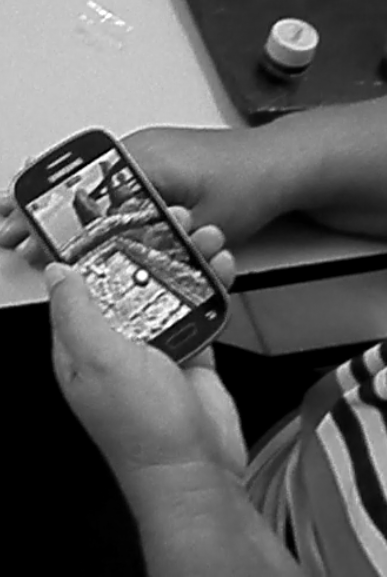
\includegraphics[scale=0.5]{./img/gametremor.png}
 % matrixargseg.png: 296x162 pixel, 100dpi, 7.52x4.11 cm, bb=0 0 213 117
 %\caption{Estágio desenvolvimento de jogos ~\cite{fullerton2008game}}
\caption{Teste de um jogo usando acelerômetro para quantificação do sinal de tremor do Parkinson}
%  \caption{Estágio desenvolvimento de jogos}
 \label{fig:gametremor}
\end{figure}

\begin{itemize}
  \item O \textbf{REQ-ENTREVISTAS-01}, o tremor de repouso é um dos principais sinais do~\ac{dp}. Sabíamos da sua importância, inclusive foi desenvolvido um jogo para \textit{Smartphone} que pudesse quantificar o tremor (Figura ~\ref{fig:gametremor}). Porém, no teste junto aos usuários, foi percebido que no momento do uso os pacientes parkinsonianos cessavam o tremor, inviabilizando assim sua quantificação. 
	\item O \textbf{[REQ-ENTREVISTAS-03]}, a técnica de \textit{finger-tapping} não pode ser avaliadas utilizando o MS-Kinnect 1.0, pois nessa versão não existe a captura do movimento dos dedos, conforme ilustrado na Figura~\ref{fig:articulacoeskinnect}.
	\item O \textbf{REQ-ENTREVISTAS-09}, por envolver estado emocional e parâmetros que não estamos levando em consideração nesse trabalho, esse requisito está fora do escopo. Entretanto, com mecanismos de detecção de batimentos cardíacos presente em versões mais atuais do MS-Kinnect, pode ser averiguada a relação dos batimentos cardíacos com o tremor.
\end{itemize}


%Em estudos prévios da nossa pesquisa, pudemos identificar esse fenômeno junto aos pacientes do~\ac{dp}, onde percebemos que os pacientes de~\ac{dp} cessavam o tremor quando confrontados com um jogo para celular desenvolvido com o propósito de quantificar o sinal do tremor (Figura~\ref{fig:gametremor}). Por esse motivo, resolvemos trabalhar com outro sinal do~\ac{dp} como a bradicinesia~\cite{protpar010} o qual pode ser avaliado utilizando um sensor de movimentos como o \textit{Ms-Kinnect Versão 1.0}~\cite{kinnect2013}. %que não necessita do contato físico do usuário além de ser utilizado em jogos eletrônicos. 



\subsubsection{Matriz de Rastreabilidade - Fragmento x Requisitos}
%\begin{center}
%\begin{table}[!htbp]
\begin{table}[!htb]
\caption{Matriz Rastreabilidade: Fragmento x Requisitos}
\label{table:matrix_rastreabilidade}
\begin{tabular}{||p{6.06cm}||ccccccccc|}
\hline
 \multicolumn{1}{|p{6.06cm}|}{\centering \textbf{FRAGMENTOS / REQUISITOS}} &  01 &  02 &  03 &  04 &  05 &  06 &  07 &  08 & 09 \\ 
\hline 
 \multicolumn{1}{|p{6.06cm}|}{\centering 01} &  x &  x &  x &  x &   &   &   &   &  \\ 
 \multicolumn{1}{|p{6.06cm}|}{\centering 02} &  x &   &   &   &   &  x &   &   &  \\ 
 \multicolumn{1}{|p{6.06cm}|}{\centering 03} &  x &  x &   &  x &  x &   &   &   &  \\ 
 \multicolumn{1}{|p{6.06cm}|}{\centering 04} &  x &   &   &   &   &   &   &   & x \\ 
 \multicolumn{1}{|p{6.06cm}|}{\centering 05} &  x &  x &   &   &   &   &   &   &  \\ 
 \multicolumn{1}{|p{6.06cm}|}{\centering 06} &   &  x &   &   &   &  x &   &   &  \\ 
 \multicolumn{1}{|p{6.06cm}|}{\centering 07} &   &  x &   &   &   &  x &  x &  x &  \\ 
 \multicolumn{1}{|p{6.06cm}|}{\centering 08} &   &  x &   &   &   &  x &  x &  x &  \\ 
 \multicolumn{1}{|p{6.06cm}|}{\centering 09} &   &   &   &  x &   &  x &   &   &  \\ 
 \multicolumn{1}{|p{6.06cm}|}{\centering 10} &   &   &   &   &   &  x &   &   &  \\ 
 \multicolumn{1}{|p{6.06cm}|}{\centering 11} &   &   &   &   &   &   &  x &   &  \\ 
 \multicolumn{1}{|p{6.06cm}|}{\centering 12} &   &  x &   &   &   &   &  x &  x &  \\ 
 \multicolumn{1}{|p{6.06cm}|}{\centering 13} &   &   &   &   &   &   &  x &   &  \\ 
 \multicolumn{1}{|p{6.06cm}|}{\centering 14} &   &  x &   &   &   &   &   &   &  \\ 
 \multicolumn{1}{|p{6.06cm}|}{\centering 15} &   &  x &   &  x &   &   &   &  x &  \\ 
 \multicolumn{1}{|p{6.06cm}|}{\centering 16} &   &   &   &  x &   &   &   &   &  \\ 
 \multicolumn{1}{|p{6.06cm}|}{\centering 17} &   &   &   &   &   &   &   &   &  \\ 
 \multicolumn{1}{|p{6.06cm}|}{\centering 18} &  x &   &  x &  x &   &  x &  x &  x & x \\ 
 \multicolumn{1}{|p{6.06cm}|}{\centering 19} &  x &   &   &   &  x &  x &  x &  x &  \\ 
 \multicolumn{1}{|p{6.06cm}|}{\centering 20} &  x &   &   &   &  x &  x &  x &  x &  \\ 
 \multicolumn{1}{|p{6.06cm}|}{\centering 21} &  x &   &   &   &  x &  x &  x &  x &  \\ 
\hline 
 \multicolumn{1}{|p{6.06cm}|}{\centering \textbf{QTD. OCORRÊNCIAS}} &  9 &  9 &  2 &  6 &  4 &  10 &  9 &  8 & 2 \\ 
\hline 
\end{tabular}
\end{table}

A Matriz de Rastreabilidade (Fragmento x Requisitos) mapeia os \textbf{REQUISITOS} aos \textbf{FRAGMENTOS} que de forma direta ou indireta estejam correlacionados (Tabela \ref{table:matrix_rastreabilidade}). Ao final, é obtido um campo de quantidade de ocorrências quantificando a sua ocorrência nos fragmentos.


%\end{center}

\subsubsection{Matriz de Rastreabilidade - Requisitos x Implementação}
A Matriz de Rastreabilidade (Tabela~\ref{table:RequisitoImplementado}) mapeia os \textbf{REQUISITOS} implementados neste trabalho e, os que devido a restrições técnicas, ainda estão em aberto. Isso demonstra também o estado atual do trabalho e pode direcionar os trabalhos futuros.

% Please remember to add \use{multirow} to your document preamble in order to suppor multirow cells
% Please remember to add \use{multirow} to your document preamble in order to suppor multirow cells
\begin{table}[h]
\centering
\caption{Requisitos Implementados}
\label{table:RequisitoImplementado}
\begin{tabular}{|c|c|c|}
\hline
\textbf{REQUISITO} & \textbf{IMPLEMENTADO} & \textbf{INVIABILIDADE TÉCNICA}\\ \hline
REQ-ENTREVISTA-01                   &                                                             & X                                                                                                                \\ \hline
REQ-ENTREVISTA-02                   & X                                                           &                                                                                                                  \\ \hline
REQ-ENTREVISTA-03                   &                                                             & X                                                                                                                \\ \hline
REQ-ENTREVISTA-04                   & X                                                           &                                                                                                                  \\ \hline
REQ-ENTREVISTA-05                   & X                                                           &                                                                                                                  \\ \hline
REQ-ENTREVISTA-06                   & X                                                           &                                                                                                                  \\ \hline
REQ-ENTREVISTA-07                   & X                                                           &                                                                                                                  \\ \hline
REQ-ENTREVISTA-08                   & X                                                           &                                                                                                                  \\ \hline
REQ-ENTREVISTA-09                   &                                                             & X                                                                                                                \\ \hline
\end{tabular}
\end{table}



\subsection{Conclusão}
Como dito no início do capítulo, o intuito dessa entrevista foi verificar junto aos profissionais de saúde os benefícios trazidos pelo monitoramento em relação a qualidade de vida e na promoção da eficácia terapêutica de seus usuários.

Com base na rastreabilidade dos fragmentos da entrevista, pode-se concluir que existiram muitas ocorrências nos requisitos de Identificação de sinais como: tremores ([\textbf{REQ-ENTREVISTAS-01}]), bradicinesia [\textbf{REQ-ENTREVISTAS-02}] e análise da marcha [\textbf{REQ-ENTREVISTAS-06}]. Para o acompanhamento e monitoramento da doença, os profissionais de saúde citaram a importância de calcular, tanto a amplitude dos movimentos de abdução e adução dos braços ([\textbf{REQ-ENTREVISTAS-07}]), quanto a velocidade angular ([\textbf{REQ-ENTREVISTAS-08}]). Baseado nessas considerações, podemos validar qualitativamente a ETAPA 1 da pesquisa.


\section{ETAPA 2: Máquina de Vetor de Suporte para Estudo Analítico de Caso Controle Por Intermédio de Sensor de Movimento Usados em Jogos Eletrônicos}\label{sec:resultado_svm}

Partindo da importância de identificar o sintoma da bradicinesia e, consequentemente, avaliar a dificuldade do movimento (Seção ~\ref{section:analise_bradicinesia}), nessa pesquisa buscou-se avaliar esse sintoma com o movimento de adução e abdução dos braços (ver Figura ~\ref{fig:movabducaomet}). A abordagem de aprendizagem de máquina foi utilizada para classificar portadores do~\ac{dp} ante indivíduos sem o diagnóstico. Partiu-se do princípio que os indivíduos com~\ac{dp} teriam mais dificuldade ao levantar o Braço e a velocidade angular do mesmo seria reduzida ante os indivíduos que não desenvolveram a doença.

\subsection{Estudo analítico de caso-controle}\label{section:estudo_caso_controle}
Esta etapa da pesquisa foi pautada pelo protocolo de pesquisa submetido à avaliação do Comitê de Ética da UFCG. Somente após a aprovação deste (\textbf{CAAE: 14408213.9.1001.5182}) é que os dados foram coletados. 

Os resultados que se pretendem alcançar com a pesquisa são mecanismos para a identificação e classificação de pessoas saudáveis ante os portadores do~\ac{dp}. Durante a pesquisa também analisou-se o sensor de movimento MS-Kinnect~\cite{kinnect2013} para avaliar a possibilidade de aquisição de dados de saúde baseada na Cinemática Linear do Movimento Humano~\cite{mcginnis2013biomechanics}. A partir dos resultados obtidos, pretende-se avaliar e classificar a normalidade e dificuldade na execução de movimentos como, por exemplo, levantar um braço~\cite{mcginnis2013biomechanics}.

A coleta de dados foi realizada no Hospital Universitário da UFAL, e na Fundação Pestalozzi em Maceió, ambas sob a tutela da Profa. e Neurologista Dra. Cícera Pontes; e na Clínica de Fisioterapia do CESMAC, sob a tutela do Prof. de Fisioterapia Jean Charles Santos. As coletas foram realizadas em local reservado e de forma individual, com a anuência do sujeito pesquisado através da assinatura do Termo de Consentimento.

\subsubsection{Amostra}
Foram selecionados por disponibilidade um total de 30 sujeitos da pesquisa. O grupo previamente diagnosticado por neurologistas com~\ac{dp} consistiu de 15 indivíduos , 10 homens e 5 mulheres, entre 51 e 65 anos (média : 58 anos) . O grupo controle foi composto por 15 indivíduos sem diagnóstico PD , 11 homens e 4 mulheres , entre 50 e 65 anos (média : 57 anos). Todos os indivíduos fizeram uso da abordagem de monitoramento baseada em jogos proposta neste trabalho. Os sujeitos da pesquisa foram solicitados a executarem os movimentos de abdução e adução dos braços de acordo com a proposta do jogo onde todas as sessões foram feitas sob supervisão de um neurologista e fisioterapeuta onde foi verificado o estado de saúde do indivíduo continuamente. Durante as coletas, não houve a necessidade de nenhuma interrupção da coleta devido a problemas de saúde ou qualquer outra eventualidade.

%A total number of 30 subjects participated in the study. The group previously diagnosed by neurologists with PD consisted of 15 subjects, 10 men and 5 women, between 51 and 65 years (mean: 58). The control group was composed of 15 subjects without a PD diagnosis, 11 men and 4 women, between 50 and 65 years (mean: 57). All subjects were interacting with exactly the same system in both hardware and software, and were prompted to seamlessly perform abduction and adduction of the arms according to the game's context. All sessions were made in a medical institution under the supervision of a neurologist or physiotherapist to continuously check the subject's health condition. No subject needed to interrupt the experiment to ensure safety.




\subsubsection{Recrutamento dos Sujeitos e Aquisição do Consentimento Livre e Esclarecido}
A forma de recrutamento deste protocolo será circunscrita por intermédio de um profissional de saúde. O profissional conhecia a história clínica do paciente e obteve a permissão do mesmo para que a equipe de pesquisa entrasse em contato. A equipe de pesquisa explicitou os riscos e benefícios da participação da pesquisa buscando a arbitrariedade e espontaneidade da decisão. Depois foi oferecido para assinatura o Termo de Consentimento Livre e Esclarecido.

\subsubsection{Critérios de Inclusão}
Foram inclusos na pesquisa, os indivíduos do grupo diagnosticados com~\ac{dp} no estágio 3 segundo a UPDRS~\cite{updrs87}, sem distinção de gênero ou cor. Os indivíduos, ficaram dentro das facilidades da clínica onde a coleta foi realizada e aceitaram participar do estudo. O grupo de indivíduos que não possuíam diagnóstico do \ac{dp}, informaram que nunca receberam o diagnóstico da doença e que aceitariam participar do estudo como grupo controle.

\subsubsection{Critérios de Exclusão}
Foram excluídos das pesquisas os indivíduos com sinais motores e que tivessem problemas de equilíbrio ou questionamento de dores ao executar os procedimentos. Foram excluídos também, o indivíduo que por qualquer motivo se negou a participar do estudo.

\subsubsection{Materiais}
Para a presente pesquisa, foram coletados movimentos de abdução e adução dos braços~\cite{mcginnis2013biomechanics}, os quais poderiam ser incorporados a um jogo eletrônico. Foi utilizado um jogo com o arcabouço de software de captura de dados desenvolvido por um aluno de Mestrado da Universidade Federal de Campina Grande~\cite{antonio2013}, juntamente a um aluno de iniciação científica do Instituto Federal de Alagoas. 

Durante a execução da coleta, houve uma preocupação com a integridade física dos participantes. Então, os movimentos utilizados no jogo foram apenas de adução e abdução dos braços~\cite{mcginnis2013biomechanics}, proporcionado a segurança dos participantes. 

%\subsubsection{Infra-Estrutura}
%A pesquisa será realizada na Clínica em que o paciente está em tratamento, onde são realizados tratamentos fisioterápicos ou consultas. O espaço físico forneceu condições favoráveis e adequadas para aplicação dos jogos. Para a realização da pesquisa foram utilizados:
%
%\begin{itemize}
	%\item Jogo (\textit{Catch the Spheres} rodando em notebook com Sistema Operacional Windows 7.0 e Unity 3d 3.0;
	%\item Projetor (Epson Lcd Powerlite X14 3000l Hdmi) para projetar o jogo na parede e facilitar a visualização;
	%\item Sensor de movimento Ms-Kinnect ~\cite{kinnect2013}.
%\end{itemize}

\subsubsection{Métodos}
Nesta pesquisa foi realizada uma análise de um sensor de movimento utilizado em jogos eletrônicos, e avaliada a possibilidade de aquisição de dados de saúde baseada na Cinemática Angular do Movimento Humano~\cite{hamill1999bases}.  Através dos resultados obtidos avaliou-se a possibilidade de classificar a normalidade e dificuldade na execução de movimentos como abdução e adução dos braços.

A coleta de dados foi realizada no próprio espaço de tratamento do indivíduo em local reservado e de forma individual. A participação do indivíduo foi consentida por meio da assinatura do Termo de Consentimento. Devido as restrições de tempo (1 minuto e 30 segundos) e da execução de um mesmo movimento por todos os participantes, foram solicitados dos voluntários a execução dos seguintes procedimentos:
\begin{enumerate}
	\item O voluntário se posiciona a uma distância de 2 metros do sensor de movimento, de modo a conseguir capturar toda a extensão superior do braço durante o movimento de abdução; 	
	\item O voluntário inicia o jogo \textit{Catch the Spheres} usando a mão esquerda conforme a interface da aplicação;
	\item O voluntário abduz e aduz 10 vezes o braço esquerdo, e depois o braço direito o mais alto e o mais rápido que consegue, de modo a permitir que fossem capturadas a amplitude de movimento e a velocidade angular do mesmo. 
	\item O voluntário fecha a aplicação e esta realiza o armazenamento dos dados.
\end{enumerate}

\begin{figure}[!htbp]
 \centering
 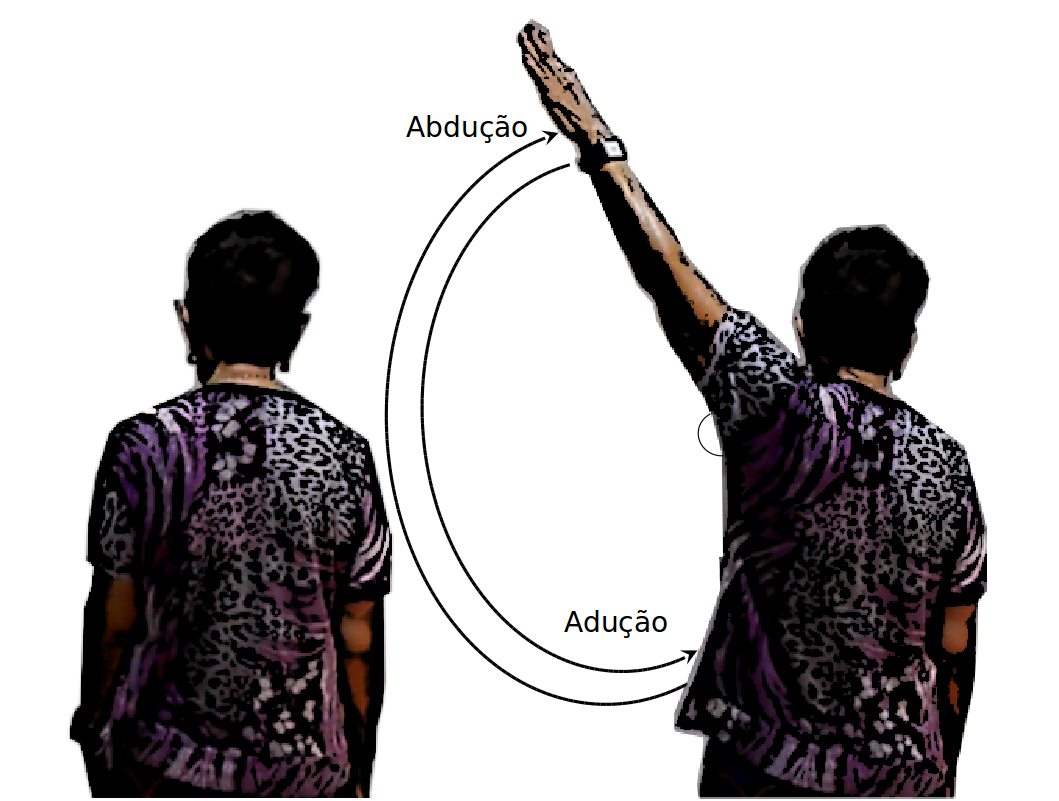
\includegraphics[scale=0.25]{./img/movaddcutctionartist2.png}
 % matrixargseg.png: 296x162 pixel, 100dpi, 7.52x4.11 cm, bb=0 0 213 117
 %\caption{Estágio desenvolvimento de jogos ~\cite{fullerton2008game}}
\caption{Movimentos de Abdução e Adução}
%  \caption{Estágio desenvolvimento de jogos}
 \label{fig:movabducaomet}
\end{figure}

Durante a análise foram comparados os Ângulos Relativos do Tronco e do Levantamento de Braços dos Indivíduos. As grandezas cinemáticas coletadas nesses estudo foram:
\begin{enumerate}
	\item Do movimento de abdução, a máxima amplitude atingida pelos membros superiores;
	\item velocidade angular de abdução membros esquerdo e direito;
	\item velocidade angular de adução membros esquerdo e direito.
\end{enumerate}

Os dados capturados desta fase resultaram na extração de características do movimento incluindo: a amplitude do movimento dos braços do lado esquerdo e direito, a velocidade angular dos movimentos de adução e abdução. A descrição dos vetores de características estão descritos na Tabela~\ref{table:features}.


\begin{table}[h]
\centering
\caption{Detalhamento do vetor de características extraído da coleta de dados.}
\label{table:features}
\begin{tabular}{|l|l|}
\hline
{\bf Característica}  & {\bf Descrição}                                       \\ \hline
MaxAmpEsquerdo     & Amplitude máxima do braço esquerdo. \\ \hline
MaxAmpDireito    & Amplitude máxima do braço direito. \\ \hline
AngVelAbdEsquerdo  & Velocidade angular do movimento de abdução do braço esquerdo. \\ \hline
AngVelAbdDireito & Velocidade angular do movimento de abdução do braço direito. \\ \hline
AngVelAdEsquerdo  & Velocidade angular do movimento de adução do braço esquerdo. \\ \hline
AngVelAdDireito & Velocidade angular do movimento de adução do braço direito. \\ \hline
\end{tabular}
\end{table}

\begin{figure}[!htb]
	\centering
	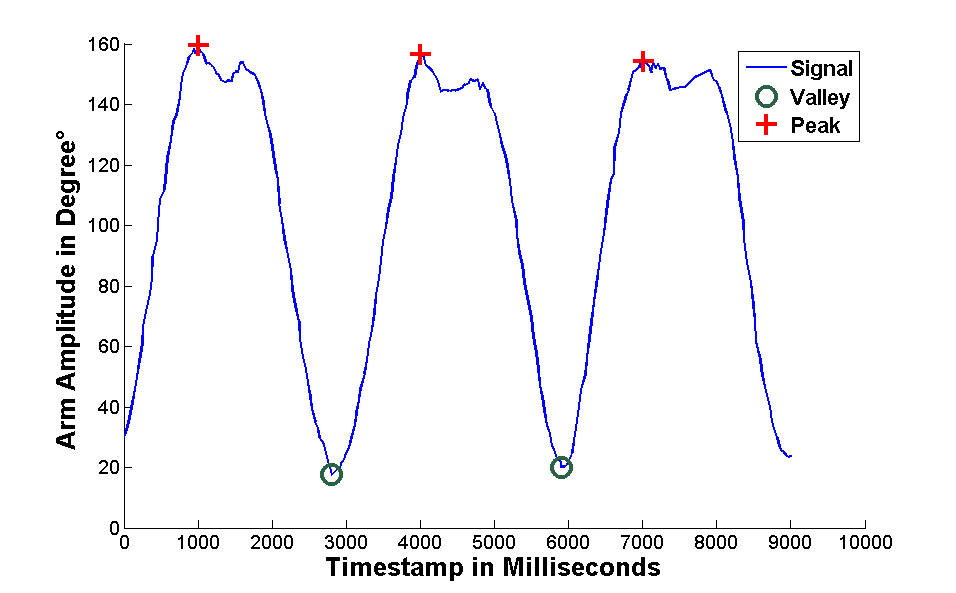
\includegraphics[width=1\textwidth]{img/signalamplitudepeakvaley-2.png}
	\caption{Exemplo do gráfico dos ângulos de adução e abdução dos braços em função do tempo}
	\label{fig:signalamplitudepeakvaley}
\end{figure}

A partir da extração das características do movimento, a próxima etapa da pesquisa é classificar os dados de movimento e identificar a ocorrência do sintoma de bradicinesia. Por meio das teorias estatísticas de aprendizagem de máquina, foi realizado uma análise dos dados para aquisição de conhecimento utilizando técnicas de aprendizagem supervisionada. 

%Logo, os dados biomecânicos~\cite{hamill1999bases} coletados foram utilizados com a \ac{dp} ante os indivíduos sem o diagnóstico estabelecido. Pelo quantitativo da pesquisa ter sido de 30 indivíduos, a abordagem de aprendizagem de máquina usando \ac{svm} ~\cite{vapnik95} foi utilizada juntamente com a técnica de validação-cruzada \textit{leave-one-out}, essa técnica será explicada com mais detalhes na Seção \ref{validacao_cruzada_svm}.


\subsubsection{Relação Risco e Benefício da Pesquisa}
Os riscos inerentes podem decorrer da exposição de dados dos sujeitos da pesquisa, o que pode acarretar danos morais e/ou psicológicos. Logo, teve-se um cuidado de preservar a integridade física e psicológica dos sujeitos da pesquisa, garantindo assim, a privacidade e confidencialidade das informações.

Caso houvesse algum constrangimento por parte do sujeito da pesquisa, ao não conseguir realizá-la ou responder alguma pergunta devido ao comprometimento da doença, os pesquisadores prestaram total assistência, orientando-o adequadamente para prosseguir ou encerrar o procedimento.

%Os presentes riscos fazem jus aos benefícios que a pesquisa venha a trazer com a possibilidade de monitoramento dos sinais da \ac{dp}. A identificação dos sinais motores e classificação desses dados através do computador podem permitir avanços para um melhor acompanhamento da evolução da doença além de possibilitar que os pacientes venham a ser monitorados de forma não invasiva através de um jogo eletrônico. Os pacientes deverão ter o seu estágio da \ac{dp} previamente diagnosticada por um médico para ser possível comparar os dados do monitoramento com a classificação obtida.




\subsection{Aplicação do Método}
O propósito da classificação é explorar a possibilidade de obter dados de saúde de forma contínua e não invasiva a partir de um sensor de captura de movimento usado em jogos eletrônicos (Ms-Kinnect). Durante a coleta dos dados foi indagado junto aos voluntários sua condição física e possíveis riscos e desconfortos que o voluntário pudesse ter ao realizar o procedimento. 

Durante a pesquisa, partiu-se do princípio, que através da análise do movimento de abdução e adução do braço, seria possível avaliar a biomecânica da amplitude do movimento dos braços e velocidade angular dos mesmos. Então, por intermédio desses dados biomecânicos, seria possível identificar a ocorrência do sintoma de bradicinesia em indivíduos portadores do \ac{dp}.



\subsection{Resultados}
Conforme a abordagem~\ac{jogue-me} apresentada no Capítulo~\ref{chapter:abordagem_gahme}, os dados adquiridos foram processados, extraídas as características do movimento angular, filtrados e postos em uma Máquina de Vetor de Suporte, para realizar a classificação entra as duas classes de dados. Para a classificação dos dados foi utilizado um \textit{kernel} Linear (Seção~\ref{sec:svm_linear}) por ter obtido os melhores resultados dentre os \textit{kernels} presentes no Matlab~\cite{matlab2011}: Polinomial, Radial e de MLP. O resultado do \textit{kernel} linear foi o mais expressivo entre os demais devido a separação linear ter dividido bem as duas classes. 

\subsubsection{Vetor Médio}
Nessa etapa da pesquisa foi calculado o Vetor Médio (Seção~\ref{section:filtro_dados}), para entender melhor a diferença de movimento entre os sujeitos diagnosticados com a \ac{dp} e sujeitos sem o diagnóstico. Como pode ser visto na Figura~\ref{fig:vetor_medio_abducao}, a amplitude de movimento de um indivíduo diagnosticado com ~\ac{dp} é bem menor do que a de um indivíduo sem o diagnóstico. Entretanto, por ter sido escalonado em 20 \textit{frames}, esse vetor médio perdeu a informação da velocidade do movimento.

\begin{figure}[!htbp]
 \centering
 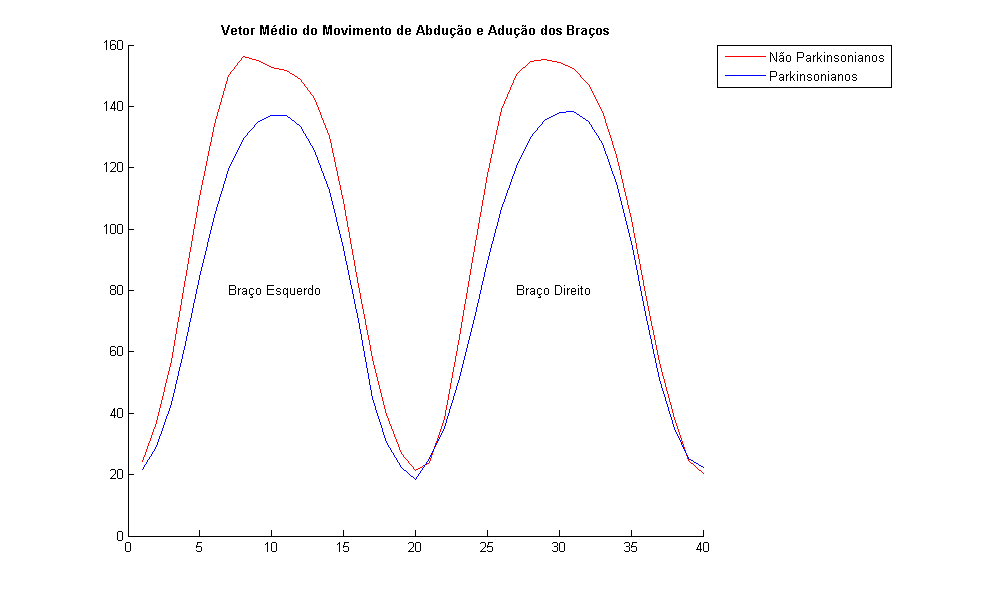
\includegraphics[scale=0.650]{./img/vetormedioaducao.png}
 \caption{Vetor Médio do Movimento de Abdução e Adução}
 \label{fig:vetor_medio_abducao}
\end{figure}

% 
% 
% \subsubsection{Validação Cruzada}\label{validacao_cruzada_svm}
% Para verificar a precisão da classificação de indivíduos saudáveis perante os parkinsonianos foi aplicada a técnica de Validação Cruzada (cross-validation) ~\cite{datamining2005}. A validação cruzada é uma técnica empregada para avaliar a capacidade de generalização de um modelo de predição em um conjunto de dados. Em um primeiro momento, realiza-se a partição do conjunto de dados em subconjuntos mutualmente exclusivos e ,posteriormente, usa-se este subconjunto para verificar a acurácia do modelo ~\cite{datamining2005}. 
% %O conceito central das técnicas de validação cruzada é o particionamento do conjunto de dados em subconjuntos mutualmente exclusivos, e posteriormente, usar alguns destes subconjuntos como dados de treinamento para encontrar valores que permitam a predição. O restante dos subconjuntos serão usados como dados de teste utilizados para avaliar o modelo preditivo.
% 
% A escolha do grupo de treinamento deve contemplar todas as classes no conjunto de dados, este procedimento é chamado de estratificação ou \textbf{Validação Cruzada Estratificada}~\cite{datamining2005}. Essa técnica é muito utilizada para mitigar a ocorrência de viés na pesquisa, pois o processo de treinamento é repetido por várias vezes com amostras diferentes incluindo diferentes casos em cada classe. Dada uma amostra única, um método de predição de taxa de erro na aprendizagem de máquina é usar a Validação-Cruzada dez vezes (\textit{10 K-Fold Cross-Validation})~\cite{datamining2005}, onde os dados são aleatórios e divididos em 10 grupos com a mesma proporção de classe. O processo de aprendizagem é executado por 10 vezes onde 1 grupo é selecionado como grupo de teste e os demais são selecionados como grupo de treinamento. A taxa de erro é calculada em cada processo de aprendizagem executado e no final é calculada a taxa de erro global. 
% 
% A escolha do número 10 para a quantidade de grupos não foi de forma aleatória, a literatura recomenda que sejam utilizados 10 grupos para obter a melhor estimativa de erro ~\cite{datamining2005}. Contudo, é reconhecido que esse número de 10 não é único ou insubstituível e em determinados casos, grupos de 5, 20 ou quaisquer outros números podem trazer melhores resultados.
% 
% Outro dado relevante para a escolha da técnica da estimativa de erro, é que uma única aplicação de Validação Cruzada \textit{10 K-Fold} pode não ser o suficiente para uma taxa de erro confiável. Pois, diferentes experimentos de Validação Cruzada podem produzir resultados distintos devido a natureza aleatória da escolha dos grupos. A estratificação reduz essa variação, contudo não a elimina completamente. Na busca por uma estimativa de erro mais exata, um procedimento que tem se transformado padrão nas técnicas de aprendizagem de máquina é repetir o processo de Validação Cruzada \textit{10 K-Fold} por 10 vezes. Ou seja, consiste em invocar o algoritmo de aprendizagem 100 vezes em um conjunto de dados, dessa forma aumenta-se a amostra de forma considerável e por consequência reduz-se a variação da taxa de erro na execução dos experimentos.
% 
% Desta maneira, o método escolhido de validação cruzada foi repetir e calcular por 10 vezes a \textit{10 K-Fold}. Os subjconjuntos são estratificados antes de cada um dos 10 processos de aprendizagem e a taxa de erro estimada em cada etapa processo de aprendizagem está exposta na Figura \ref{fig:erroestimadopca}. A taxa de classificação global é a média da taxa de acerto calculada em todo o processo.


\subsubsection{Matriz de Confusão e Suas Métricas}
Para avaliar o resultado da classificação, será apresentada a \textbf{matriz de confusão}~\cite{datamining2005}, que permite comparar os valores reais da classe com os valores obtidos no modelo de predição. 

A matriz de confusão para duas classes consiste numa matriz $2$\ x $2$\, contendo os \textit{Verdadeiros Positivos} (\textbf{TP}) e \textit{Verdadeiro Negativo} (\textbf{TN}), que são as classificações corretas. Os \textit{Falsos Negativos} (\textbf{FN}) contém a predição incorreta de um valor que deveria ser positivo e os \textit{Falsos Positivos} (\textbf{FP}) contém os valores positivos quando deveriam ser negativos como pode ser visto na Tabela~\ref{table:descricaomatrizconfusao}.

% Please remember to add \use{multirow} to your document preamble in order to suppor multirow cells
\begin{table}[!htbp]
\caption{Descrição da Matriz de Confusão}
\label{table:descricaomatrizconfusao}
\begin{tabular}{ll|c|c|}
\cline{3-4}
                                                                                                               & \multicolumn{1}{c}{}                         & \multicolumn{2}{|c|}{\textit{\textbf{Classe Preditiva}}} \\ \cline{3-4} 
                                                                                                               &                                              & \textbf{Parkinson}          & \textbf{Não Parkinson}     \\ \hline
\multicolumn{1}{|c}{\multirow{\textit{\textbf{\begin{tabular}[c]{@{}c@{}}Classe\\ Atual\end{tabular}}}}} & \multicolumn{1}{|l|}{\textbf{Parkinson}}     & Verdadeiros Positivos (VP)  & Falsos Negativos (FN)      \\ \cline{2-4} 
\multicolumn{1}{|l}{\textit{\textbf{}}}                                                                        & \multicolumn{1}{|l|}{\textbf{Não Parkinson}} & Falsos Positivo (FP) & Verdadeiros Negativos (VN) \\ \hline
\end{tabular}
\end{table}

% 
% A matriz de confusão é uma ferramenta importante para avaliar os resultados de predição, pois facilita o entendimento do que está sendo avaliado e como se comporta o classificador em relação aos erros de classificação obtidos. Esta matriz serve como base para métricas que podem ser aplicadas a classificação e,  consequentemente, exibem a precisão do modelo. A matriz desta pesquisa (Tabela ~\ref{table:resultadomatrizconfusaopca}) foi gerada a partir da repetição de dez vezes da técnica de Validação Cruzada \textit{10-K-Fold}, conforme a Seção \ref{sec:validacao_cruzada_database}.
% 
% \begin{table}[!htbp]
% \caption{Resultado da Matriz de Confusão}
% \label{table:resultadomatrizconfusaopca}
% \centering
% \begin{tabular}{l|c|c|}
% \cline{2-3}
% \multicolumn{1}{c}{}                         & \multicolumn{2}{|c|}{\textit{\textbf{Classe Preditiva}}} \\ \cline{2-3} 
%                                              & \textbf{Parkinson}      & \textbf{Não-Parkinson}         \\ \hline
% \multicolumn{1}{|l|}{\textbf{Parkinson}} & 429       & 71           \\ \hline
% \multicolumn{1}{|l|}{\textbf{Não Parkinson}}     & 114           & 386     \\ \hline
% \end{tabular}
% \end{table}
% 


\subsection{Aprendizagem de Máquina (SVM)}

Para uma base de dados pequena contendo 30 indivíduos, o método de Validação Cruzada escolhido deve tentar maximizar o conjunto de treinamento para atingir um melhor resultado de teste. Por esse motivo, foi escolhido o método de validação cruzada \textit{leave-one-out}. 

O método \textit{leave-one-out} é um método de validação cruzada \textit{k-fold} com o mesmo número de \textit{n} indivíduos. Logo, apenas um indivíduo será considerado teste e os demais serão de treinamento. Desta maneira não existe estratificação nos dados, tornando o processo determinístico e repetível com a mesma base de dados, pois não existe o problema de viés na seleção dos dados. A taxa de erro obtida da classificação é a taxa de erro do modelo para aquela base de dados. 

\subsubsection{Otimização dos Parâmetros da SVM - Método Grid-Search}

Para identificar os melhores parâmetros~\ac{svm}, foi aplicada a técnica~\cite{gridsearchsvm2010} usando validação cruzada \textit{Leave-One-Out} (LOOCV)~\cite{datamining2005}. Esta técnica avalia a precisão do modelo prevista , evita o problema superajuste na classificação binária e é um método prático para identificar os parâmetros SVM . Neste estudo, para reduzir a taxa de erro , nós aplicamos uma abordagem minimax para maximizar a margem sobre os coeficientes hiperplano ea classificação correta. Os valores dos parâmetros de pesquisa do \textit{grid-search} foi de: $C$ = [$2^5$, ... ,$2^2$] e $\gamma$ = [$2^{15}$, ... ,$2^3$ ] usando assim uma exponencial de base 2. Por meio desta técnica foi possível identificar uma região em que o classificador possuía a melhor acurácia e menor taxa de \textit{FpRate}. Após identificar essa região realizamos uma busca mais detalhada utilizando a técnica de \textit{grid-search} com os seguintes parâmetros: $C$ = [0.25, 0.5, ... ,2.5]; e $\gamma$ = [1, 2, ...,10] como 
pode ser visto na Figura~\ref{fig:gridaccuracy}.

%To identify the best SVM parameters, we applied the grid search technique~\citep{gridsearchsvm2010} using Leave-One-Out Cross-Validation (LOOCV)~\citep{datamining2005}. This technique assesses the accuracy of the predicted model, prevents the overfitting problem in the binary classification and is a practical method to identify the SVM parameters. In this study, to reduce the error rate, we applied a minimax approach to maximize the margin over the hyperplane coefficients and the correct classification. The parameters values of grid search for $C$ = [$2^5$, ... ,$2^2$] and $\gamma$ = [$2^{15}$, ... ,$2^3$ ], the step length was $2^2$, and with the identification and selection of a “better” region on the grid. So, we did a finer 


\begin{figure}[!h]
 \centering
 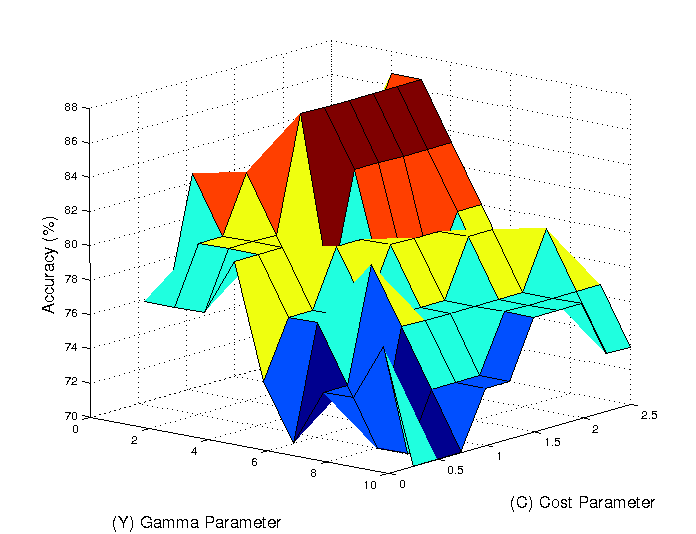
\includegraphics[scale=0.7]{./img/gridsearch.png}
 % matrixargseg.png: 296x162 pixel, 100dpi, 7.52x4.11 cm, bb=0 0 213 117
 %\caption{Estágio desenvolvimento de jogos ~\cite{fullerton2008game}}
\caption{\textit{Grid-Search} - Acurácia da Classificação}
%  \caption{Estágio desenvolvimento de jogos}
 \label{fig:gridaccuracy}
\end{figure}



% \begin{figure*}[htbp!]
% \subfigure[\textit{Grid-Search} - Acurácia da Classificação.]{
% 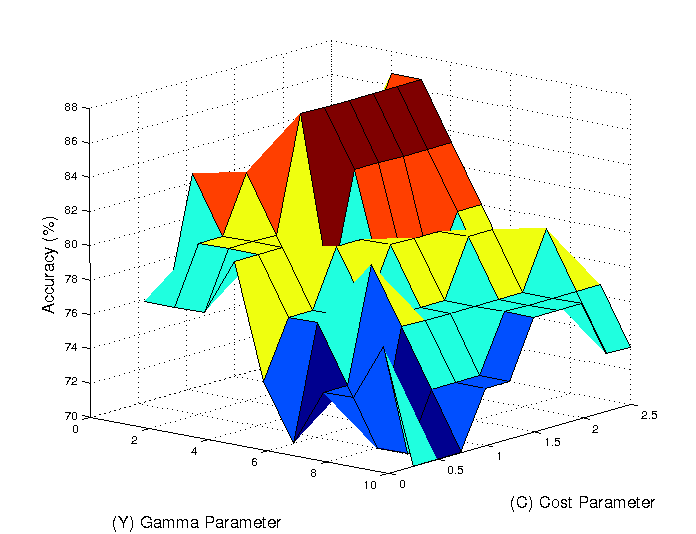
\includegraphics[scale=0.4]{./img/gridsearch.png}
% \label{fig:gridaccuracy}
% }
% \subfigure[Grid Search - FPRate.]{
% 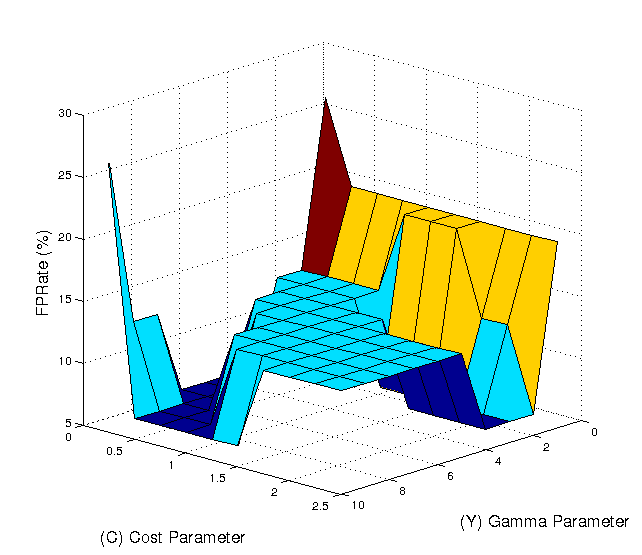
\includegraphics[scale=0.4]{./img/gridsearchfprate.png}
% \label{fig:gridfprate}
% }
% \label{fig:gridsearch}
% \caption{GridSearch for SVM Parameter Optimization.}
% \end{figure*}
% 
Como pode ser analisado na Figura~\ref{fig:gridaccuracy}, nós conseguimos uma classificação nos dados em que a pior seleção obteve uma acurácia de 70,00\% e melhor de 86,67\%. Conseguimos também um baixo valor de \textit{FpRate} com 6,67\% no melhor dos casos (Figura~\ref{fig:gridfprate}). Usando a técnica de \textit{grid-search} nós encontramos como melhor valor para os parâmetros: $C = 2$ and $\gamma = 3$. Como podemos analisar nos nossos resultados, por meio da técnica \textit{grid-search} foi possível identificar parâmetros para o classificador~\ac{svm} com uma boa generalização e que foi capaz de identificar a maior \textit{acurácia} e e menor nível de \textit{FpRate}.


\begin{figure}[!h]
 \centering
 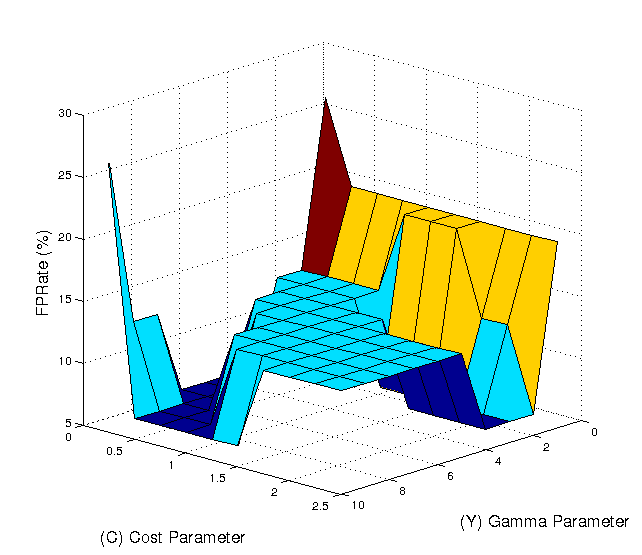
\includegraphics[scale=0.7]{./img/gridsearchfprate.png}
 % matrixargseg.png: 296x162 pixel, 100dpi, 7.52x4.11 cm, bb=0 0 213 117
 %\caption{Estágio desenvolvimento de jogos ~\cite{fullerton2008game}}
\caption{\textit{Grid-Search} - \textit{FpRate}}
%  \caption{Estágio desenvolvimento de jogos}
 \label{fig:gridfprate}
\end{figure}


%As illustrated in Fig.~\ref{fig:gridaccuracy}, we achieved a good classification performance where the worst accuracy was 70.00$\%$ and the best was 86.67$\%$. We obtained very low values for False Positives (FP), with 6.67$\%$ of \textit{FPRate} on the best fit (Fig.~\ref{fig:gridfprate}). This way, $C = 2$ and $\gamma = 3$ were the best kernel parameters, achieving accurate classification and minimizing the \textit{FPRate}. 

%The best classification performance of this study is presented in the confusion matrix for two classes that consist of a matrix $2$\ x $2$\, with (TP, FP, TN and FN) described in Table~\ref{table:resultadomatrizconfusaosvm}. True Positive (TP) indicates correctly classified with abnormal movement.  True Negative (TN) indicates correctly classified with normal movement. False Positives (FP) indicate the normal movement classified as abnormal ones and the False Negatives (FN) indicate the real abnormal movement not correctly detected. 

%Table~\ref{table:metricas} shows the classification performance, where the \textit{TpRate} is TP divided by the total number of positives, which is TP + FN; the \textit{FpRate} is FP divided by the total number of negatives, which is FP + TN. The \textit{Accuracy} is the number of correct classifications divided by the total number of classifications~\citep{datamining2005}.

%\subsection{Técnicas de Otimização da SVM}



%
%\begin{figure}
 %\centering
 %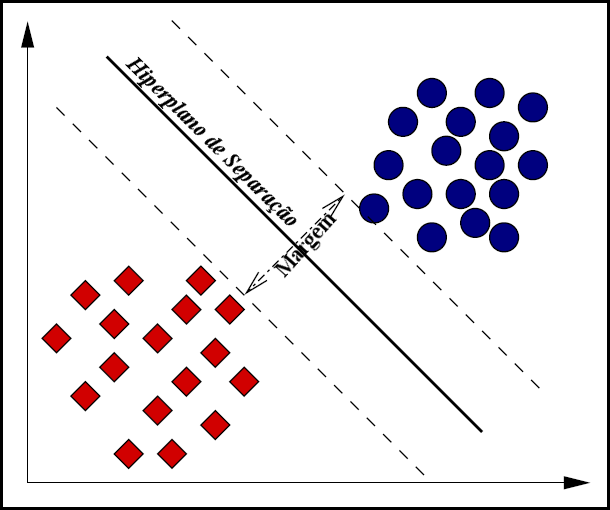
\includegraphics[scale=0.4]{./img/svmhyperplane.png}
 %% matrixargseg.png: 296x162 pixel, 100dpi, 7.52x4.11 cm, bb=0 0 213 117
 %%\caption{Estágio desenvolvimento de jogos ~\cite{fullerton2008game}}
%\caption{Hiperplano de Separação Linear Para Duas Classes}
%%  \caption{Estágio desenvolvimento de jogos}ETAPA 3 - Avaliação Da Aceitação Da Abordagem Junto aos Pacientes de~\ac{dp} Utilizando \textit{Goal Question Metric}
 %\label{fig:hiperplano}
%\end{figure}
%
%
%
%
%A aprendizagem supervisionada consiste em que dado um conjunto de dados para treinamento 
%
%O modelo mais simples de ~\ac{svm},foi o primeiro a ser desenvolvido, foi chamado de Classificador de Margem Máxima, o qual trabalha apenas com dados linearmente separáveis, ficando restrito a essas aplicações. Contudo, apesar dessa restrição o Classificador de Margem Máxima possui propriedades importante que foram fundamentais para a elaboração de SVMs mais eficazes ~\cite{svm-cg-2002}. 
%
%\begin{figure}
 %\centering
 %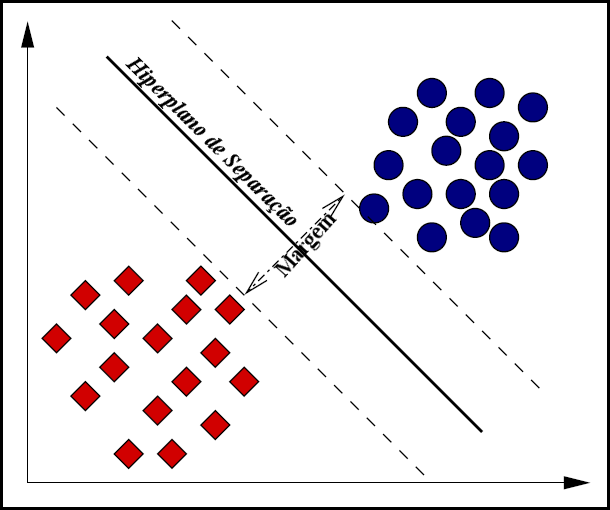
\includegraphics[scale=0.4]{./img/svmhyperplane.png}
 %% matrixargseg.png: 296x162 pixel, 100dpi, 7.52x4.11 cm, bb=0 0 213 117
 %%\caption{Estágio desenvolvimento de jogos ~\cite{fullerton2008game}}
%\caption{Hiperplano de Separação Linear Para Duas Classes}
%%  \caption{Estágio desenvolvimento de jogos}
 %\label{fig:hiperplano}
%\end{figure}
%
%Pode ser visto na Figura ~\ref{fig:hiperplano_linear_separavel} uma projeção de dados bidimensionais temos a representação de um conjunto de dados de treinamento  bidimensional e sua separação linear a separação dos dados pode ser realizada linearmente 
%
%\begin{figure}
 %\centering
 %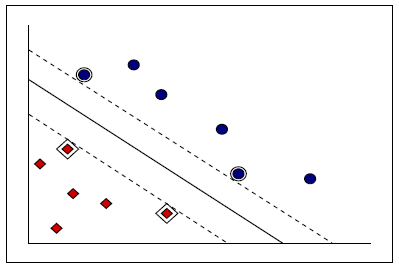
\includegraphics[scale=0.4]{./img/hiperplano-linear.png}
 %% matrixargseg.png: 296x162 pixel, 100dpi, 7.52x4.11 cm, bb=0 0 213 117
 %%\caption{Estágio desenvolvimento de jogos ~\cite{fullerton2008game}}
 %\caption{Espaço de Características Linearmente Separável ~\cite{svm-cg-2002}}
%%  \caption{Estágio desenvolvimento de jogos}
 %\label{fig:hiperplano_linear_separavel}
%\end{figure}
%
%\begin{figure}
 %\centering
 %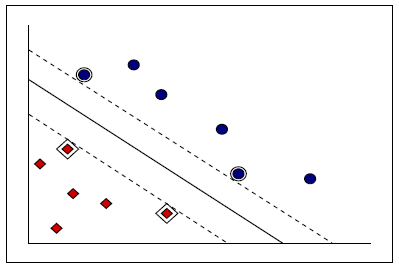
\includegraphics[scale=0.4]{./img/hiperplano-linear.png}
 %% matrixargseg.png: 296x162 pixel, 100dpi, 7.52x4.11 cm, bb=0 0 213 117
 %%\caption{Estágio desenvolvimento de jogos ~\cite{fullerton2008game}}
 %\caption{Espaço de Características Linearmente Inseparável ~\cite{svm-cg-2002}}
%%  \caption{Estágio desenvolvimento de jogos}
 %\label{fig:linear-inseparavel}
%\end{figure}
%
%
%
%% Vapnik idealizou o princípio indutivo de Minimização do Risco Estrutural. Este princípio busca minimizar o erro do conjunto de treinamento (risco empírico), juntamente com o erro do conjunto de teste \cite{svm-cg-2002}.
%
%Formalmente, classificadores que separam os dados por meio de um hiperplano de Equação(~\ref{eq:hiperplano}) são denominados discriminante linear~\cite{valt2010}.
%\linebreak
%\begin{equation}
%f(x)=w^Tx+b=0
%\label{eq:hiperplano}
%\end{equation}.



\subsubsection{Resultados Obtidos}
A Matriz de Confusão obtida indica que existem três indivíduos classificados como ``Não-Parkinson'' e que possuem a doença, no entanto analisando as características do movimento desses indivíduos ``Parkinsonianos'' percebemos que eles possuíam uma amplitude de movimento e uma velocidade angular bastante próximas dos indivíduos do Grupo Controle. Logo, estes não apresentam o sintoma de bradicinesia, o que pode indicar que o indivíduo esteja no início da doença, ou bem medicado, ou inclusive não apresentar este sinal motor o que está adequada a sintomatologia do~\ac{dp}. 
Um resultado, que não era esperado nesta pesquisa é a ocorrência de um indivíduo que não possui~\ac{dp} mas mesmo assim foi classificados com o sintoma. Analisando seus dados foi percebido que ele possuía sinais muito próximos do grupo dos indivíduos com~\ac{dp}, logo ele possivelmente apresenta algum déficit motor o que condiz com o resultado da classificação.

\begin{table}[!htbp]
\caption{Resultado da Matriz de Confusão SVM}
\label{table:resultadomatrizconfusaosvm}
\centering
\begin{tabular}{l|c|c|}
\cline{2-3}
\multicolumn{1}{c}{}                         & \multicolumn{2}{|c|}{\textit{\textbf{Classe Preditiva}}} \\ \cline{2-3} 
                                             & \textbf{Parkinson}      & \textbf{Não-Parkinson}         \\ \hline
\multicolumn{1}{|l|}{\textbf{Parkinson}} & 12       & 3           \\ \hline
\multicolumn{1}{|l|}{\textbf{Não Parkinson}}     & 1           & 14     \\ \hline
\end{tabular}

\end{table}


 Para demonstrar a avaliação do modelo de forma quantitativa usou-se um conjunto de métricas derivadas da matriz de confusão ~\cite{datamining2005}.
 \begin{description}
 	\item [\textit{TpRate}] taxa de acerto obtido: $ TpRate = TP/P $\ ;
 	\item [\textit{FpRate}]: taxa de falso alarme obtido: $ FpRate = FP/N $\ ;
 	\item [\textit{Precision}]: taxa de acerto de uma instância em determinada classe: $ Precision =  TP/(TP +FP) $\ ;
 	\item [\textit{Accuracy}]: taxa de acerto de todo o classificador: $ Accuracy = (TP+TN)/(P+N) $\ ;
 	\item [\textit{F-Measure}]: análise de classificador binário que mede a acurácia do teste. Considerando a média harmônica da taxa de \textit{precision} e do \textit{tp rate}: $ F-Measure = 2 * (Precision * TpRate)/(Precision + TpRate) $\ .
 \end{description}



\begin{table}[!htbp]
\label{table:metricasmatrizconfusao}
\caption{Métricas da Matriz de Confusão}
\centering
\begin{tabular}{|l|r|}
\hline
\multicolumn{2}{|l|}{\textbf{Métricas}} \\ \hline
\textbf{TpRate}                    & 80,00$\%$\                 \\ \hline
\textbf{FpRate}                    & 6,67$\%$\                \\ \hline
\textbf{Precision}                 & 92,31$\%$\                \\ \hline
\textbf{Accuracy}                  & 86,67$\%$\                \\ \hline
\textbf{F-Measure}                 & 85,71$\%$\                \\ \hline
\end{tabular}
\end{table}






\subsubsection{Limitações do Método}
O método utilizado para diferenciar os movimentos executados de indivíduos diagnosticados com \ac{dp} ante os indivíduos sem o diagnóstico estabelecido, foi uma técnica estatística de aprendizagem denominada de~\ac{svm}. Nesse estudo não se pretende estabelecer um diagnóstico da \ac{dp}, ou até mesmo provar que os movimentos utilizados pelos participantes da pesquisa servem para um diagnóstico. Contudo, este trabalho demonstra que existem diferenças entre essas duas classes, e estas podem ser capturadas por um sensor de movimento usado em jogos eletrônicos, e que essas diferenças podem ser classificadas utilizando uma abordagem de aprendizagem de máquina. 

\section{ETAPA 3 - Avaliação Da Aceitação Da Abordagem Junto aos Pacientes de~\ac{dp} Utilizando \textit{Goal Question Metric}}\label{gqm_usuarios}
%Para identificar a possibilidade de integrar o monitoramento da saúde do jogador através de jogos eletrônicos à sua rotina diária, foi utilizada a abordagem \textit{Goal, Question, Metric} (GQM). GQM ~\cite{basili94} é uma abordagem hierárquica que inicia com objetivo principal e o divide em atividades que podem ser mensuradas durante a execução do projeto. É uma abordagem para integrar objetivos a e perspectivas de qualidade de interesse, baseado nas necessidades do projeto~\cite{van1999goal}. Foi preparado o questionário GQM mostrado no Apêndice~\ref{apend:gqm} para avaliar a possibilidade de monitorar dados motores de forma não invasiva e integrada a rotina diária das pessoas.

Com o objetivo de averiguar a possibilidade de integrar o monitoramento da saúde do jogador através de jogos eletrônicos à sua rotina diária, foi utilizada a abordagem \textit{Goal, Question, Metric} (GQM)~\cite{van1999goal}. Essa abordagem é um paradigma de pesquisa utilizado na Engenharia de Software para medição de processos de software e melhoria contínua dos produtos ~\cite{saraiva2006,elicquest05}. A qualidade do produto de software~\cite{saraiva2006} pode ser compreendida como a adequação a um conjunto de características atingidas em maior ou menor grau para que o produto final venha atender as necessidades do usuário final, identificadas na fase de elicitação de requisitos ~\cite{elicquest05}.

O~\ac{gqm} é um paradigma de avaliação orientado por metas e tem como componentes elementares: objetivos, questionamentos e a métricas ~\cite{saraiva2006}. Nesse paradigma de pesquisa é definido um objetivo principal, onde são refinados em perguntas que venham extrair as métricas da pesquisa que fornecem informações. De posse das respostas baseada em métricas, estas são comparadas com o objetivo da pesquisa no intuito de identificar se ele foi alcançado. Logo, o paradigma~\ac{gqm} busca definir métricas partindo de uma perspectiva de ``de cima para baixo''; analisa, interpreta e mensura dados de maneira ``de baixo para cima'' como pode ser graficamente visualizado na Figura~\ref{fig:gqm} ~\cite{van1999goal}. 

\begin{figure}[!htbp]
 \centering
 \includegraphics[scale=0.50]{./img/gqm.png}
 \caption[O Paradigma GQM \copyright]{O Paradigma GQM \copyright~\cite{van1999goal}}
 \label{fig:gqm}
\end{figure}

Segundo Saraiva ~\cite{saraiva2006}, numa análise da aplicação do método de ~\ac{gqm} para o contexto de avaliação de usabilidade de software, os componentes elementares do paradigma ~\ac{gqm} são:

\begin{itemize}
	\item \textbf{Objetivo}: Sua definição envolve o propósito da avaliação, o que deve ser avaliado, a perspectiva e o ambiente proposto.
	\item \textbf{Questão}: A questão anuncia a necessidade de se obter informações em linguagem natural, podendo formular uma ou mais questões para cada categoria. Logo, sua resposta deve estar condicionada ao objetivo proposto.
	\item \textbf{Métrica}: Sua função é especificar os dados que se deseja obter durante as avaliações em termos quantitativos, podendo ter mais de uma métrica para cada questão.	
\end{itemize}

Baseado nos componentes elementares do paradigma, foi elaborado um questionário~\ac{gqm} (Apêndice~\ref{apend:gqm}) com o objetivo principal de avaliar a possibilidade de monitorar dados motores, de forma não invasiva e integrada a rotina diária dos usuários. Para elaboração de métricas para atingir esse objetivo foram formuladas duas questões de pesquisa com o intuito de avaliar:
\begin{enumerate}
	\item se o usuário integraria a abordagem~\ac{jogue-me} à sua rotina diária;
	\item se a segurança com a integridade física está de acordo com a faixa etária do usuário.
\end{enumerate}

O questionário consistiu de um conjunto de 10 questões de resposta fechada (quantitativa) ~\cite{elicquest05}, e o entrevistado deve escolher uma resposta dentre as alternativas dadas. Esse método foi escolhido para contribuir por uma maior uniformidade nas respostas e consequentemente facilitar sua análise. Porém, este método impede a expressão das opiniões dos entrevistados~\cite{elicquest05}. 

%\begin{table}
%\begin{longtable}{|p{\textwidth}|}
%\caption{O Questionário GQM}\\
%\label{table:table_gqm}
%\hline
%\endfirsthead
%\multicolumn{1}{c}%
%{\tablename\ \thetable\ -- \textit{Continuação da página anterior}} \\
%\hline
%\endhead
%\hline \multicolumn{1}{r}{\textit{Continua na próxima página}} \\
%\endfoot
%\hline
%\endlastfoot
%\textbf{\textit{Objetivo principal}}: Avaliar a possibilidade de monitorar dados motores de forma não invasiva e integrada a rotina diária das pessoas. \\ \hline
%\textbf{\textit{Questão 1}}: O usuário poderia integrar a abordagem \textit{HGMS-E} à sua rotina diária ?\\ \hline
%\textit{Métrica 1.1}: Numa escala de 1 a 5 qual o grau de diversão do jogo? \\ \hline
%\textit{Métrica 1.2}: O jogo traz motivação ao usuário ? (Sim/Não) \\ \hline
%\textit{Métrica 1.3}: Se o usuário tivesse adquirido esse jogo, com que frequência o utilizaria durante a semana? (1 vez/3 vezes/Todos os dias/Nunca usaria) \\ \hline
%\textit{Métrica 1.4}: O usuário considera o jogo simples, sem muitas regras e de fácil entendimento ? Ele pode ser aplicado em diferentes idades? (Sim/ Não) \\ \hline
%\textit{Métrica 1.5}: O usuário tem o costume de jogar esses jogos casuais em casa? (Sim/ Não) \\ \hline
%\textit{Métrica 1.6}: O usuário agregaria um jogo desse estilo em sua rotina diária? (Sim/ Não) \\ \hline
%\textbf{\textit{Questão 2}}: A segurança com a integridade física está de acordo com a faixa etária do usuário ? \\ \hline
%\textit{Métrica 2.1}: Uma criança estaria segura jogando esse jogo, ao efetuar os movimentos dos braços? \\ \hline
%\textit{Métrica 2.2}: Um adulto estaria seguro ao jogar esse jogo, ao efetuar os movimentos dos braços? \\ \hline
%\textit{Métrica 2.3	}: Um idoso estaria seguro ao jogar esse jogo, ao efetuar os movimentos dos braços? \\ \hline
%\textit{Métrica 2.4}: Qual opinião do usuário sobre a faixa etária do jogo? (Livre/Crianças/Adultos/Idosos) \\ \hline
%\end{longtable}
%\end{center}
%\end{table}


\subsection{Aplicação do Método}
%A abordagem de ~\ac{GQM}, tem o intuito de auxiliar na elaboração de planos de avaliação de atributos de qualidade de produtos e processos de software ~\cite{basili94}. Sabemos, que essa abordagem é muito mais empregada na avaliação de processos, porém nessa pesquisa iremos invocar a técnica para a avaliação do produto do ponto de vista do usuário. Essa abordagem, permite identificar métricas apropriadas ao contexto e objetivos da avaliação de modo a facilitar a interpretação e análise dos dados orientados por metas.
%
%Essa etapa da pesquisa teve como objetivo avaliar se os possíveis usuários do sistema iriam aprovar o monitoramento motor usando jogos eletrônicos. Essa avaliação vai ao encontro do usuário final e principal beneficiado pela abordagem apresentada nessa proposta de Tese.

%Essa etapa da pesquisa foi realizada em colaboração com o trabalho de Santos Jr. ~\cite{antonio2013}, que desenvolveu também o mecanismo de captura dos dados Seção~\ref{sec:cliente_game}.  Tendo como objetivo avaliar se possíveis usuários do sistema iriam aprovar o monitoramento motor usando jogos eletrônicos. Essa avaliação vai ao encontro do usuário final e principal beneficiado pela abordagem apresentada nessa proposta de Tese.

Nessa etapa da pesquisa foram entrevistadas 24 pessoas do Laboratório Embedded da Universidade Federal de Campina Grande, do Instituto Federal de Alagoas, e em pacientes da Fundação Pestalozzi e da clínica de Fisioterapia do CESMAC (ambas em Maceió). Os usuários foram selecionados para jogar o \emph{Catch the Spheres} (Seção ~\ref{jogo_catch}), testaram e responderam o questionário para verificar a aceitabilidade da solução junto aos usuários. 

%Buscou-se também validar a viabilidade da Arquitetura de Software do \textit{\textit{HGMS-E}}, verificando a possibilidade de capturar dados motores. 
O procedimento para executar as sessões de teste foi:
\begin{enumerate}
	\item O usuário se posicionou a uma distância de 2 metros do sensor de movimento, de modo a adquirir toda a extensão superior do braço; 	
	\item O usuário iniciou o jogo \textit{Catch the Spheres}, conforme a interface da aplicação;
	\item O usuário utilizou o jogo \textit{Catch the Spheres} por volta de 00:01:30s;
	\item O usuário fechou a aplicação.
\end{enumerate}

\subsection{Resultados}
Os resultados do questionário são apresentados na Tabela ~\ref{table:resultados_gqm} contendo as respostas binárias ``Sim/Não'' e nas Figuras~\ref{fig:question1},\ref{fig:question3},\ref{fig:question10} nas perguntas de questões com múltipla escolha.

\textit{Questão 1 - O usuário poderia integrar a abordagem~\ac{jogue-me} à sua rotina diária ?}: os 24 usuários deram as seguintes respostas nas Métricas (1.1, 1.2, 1.3,1.4,1.5 e 1.6): 75\% dos usuário atribuíram ao menos nota 4 (de 1 a 5) ao grau de diversão do jogo; 91,67\% sentiram motivados com o jogo; 58\% dos usuários jogariam 3 vezes por semana, 25\% jogariam todos os dias e apenas 17\% jogariam uma vez por semana. 

Então, tem-se um percentual de 83\% de usuários que poderiam integrar o monitoramento motor a sua rotina; 91,67\% consideraram o jogo simples e de fácil entendimento, e isso permite o uso de um maior número de usuários. Uma métrica desfavorável foi que apenas 41,67\% dos usuários possuem o costume de usar jogos casuais em casa. Mas, devido a expectativa de melhora do estado de saúde, 75\% dos usuários responderam que agregariam o jogo a sua rotina diária.

\textit{Questão 2 - A segurança com a integridade física está de acordo com a faixa etária do usuário
?}: nesta questão percebe-se uma grande preocupação dos usuários quanto a risco de quedas. Inicialmente, a pesquisa seria destinada para o movimento de braços e pernas. Devido aos riscos, foi modificada para movimentação somente dos braços, reduzindo a preocupação dos usuários. Mesmo assim, as métricas obtidas demonstraram que o jogo é seguro para crianças e adultos. No caso dos idosos, 75\% dos usuários consideraram o jogo seguro para essa faixa etária, muito embora os mesmos usuários classificaram o jogo com a faixa etária ``livre'', com 88\% de ocorrência.

% Please remember to add \use{multirow} to your document preamble in order to suppor multirow cells
\begin{table}[h]
\caption{Métricas Avaliadas do \textit{GQM}}
\centering
\begin{tabular}{|p{10cm}|p{1.2cm}|p{1.2cm}|}
\hline
\textbf{Métrica} & \textbf{Sim} & \textbf{Não} \\ \hline
1.2: O jogo traz motivação ao usuário? & 91,67\% & 8,33\% \\ \hline
1.4: O usuário considera o jogo simples, sem muitas regras e de fácil entendimento? Ele pode ser aplicado em diferentes idades? & 91,67\% & 8,33\% \\ \hline
1.5: O usuário tem o costume de jogar esses jogos casuais em casa? & 41,67\% & 58,33\% \\ \hline
1.6: O usuário agregaria um jogo desse estilo em sua rotina diária? & 75\% & 25\% \\ \hline
2.1: Uma criança estaria segura jogando esse jogo, ao efetuar os movimentos dos braços? & 100\% & 0\% \\ \hline
2.2: Um adulto estaria seguro ao jogar esse jogo, ao efetuar os movimentos dos braços? & 100\% & 0\% \\ \hline
2.3: Um idoso estaria seguro ao jogar esse jogo, ao efetuar os movimentos dos braços? & 75\% & 25\% \\ \hline
\end{tabular}
\label{table:resultados_gqm}
\end{table}


\begin{figure}[!htb]
     \centering
     \includegraphics[scale=0.7]{./img/chart_1-.png}
     \caption{Resultado da Pergunta 1}
     \label{fig:question1}
\end{figure}


\begin{figure}[!htb]
     \centering
     \includegraphics[scale=0.7]{./img/chart_3-.png}
     \caption{Resultado da Pergunta 3}
     \label{fig:question3}
\end{figure}


\begin{figure}[!htb]
     \centering
     \includegraphics[scale=0.7]{./img/chart_10-.png}
     \caption{Resultado da Pergunta 10}
     \label{fig:question10}
\end{figure}
\FloatBarrier




%\begin{figure}
        %\centering
        %\begin{subfigure}[b]{0.3\textwidth}
                %\centering
                %\includegraphics[width=\textwidth]{./img/chart_1.png}
                %\caption{Pergunta 1 (1: 0\%; 2: 6\%; 3: 28\%; 4: 61\%; 5: 6\%)}
                %\label{fig:question1}
        %\end{subfigure}%
        %~ %add desired spacing between images, e. g. ~, \quad, \qquad etc.
          %%(or a blank line to force the subfigure onto a new line)
        %\begin{subfigure}[b]{0.3\textwidth}
                %\centering
                %\includegrapResultado Obtidoshics[width=\textwidth]{./img/chart_2.png}
                %\caption{Pergunta 2 (Sim: 67\%; Não: 33\%)}
                %\label{fig:question2}
        %\end{subfigure}
        %~
        %\begin{subfigure}[b]{0.3\textwidth}
                %\centering
                %\includegraphics[width=\textwidth]{./img/chart_3.png}
                %\caption{Pergunta 3 (1 vez: 28\%; 3 vezes: 61\%; Todos os dias: 11\%; Nunca: 0\%)}
                %\label{fig:question3}
        %\end{subfigure}
%
        %\begin{subfigure}[b]{0.3\textwidth}
                %\centering
                %\includegraphics[width=\textwidth]{./img/chart_4.png}
                %\caption{Pergunta 4 (Sim: 100\%)}
                %\label{fig:question4}
        %\end{subfigure}
        %~
        %\begin{subfigure}[b]{0.3\textwidth}
                %\centering
                %\includegraphics[width=\textwidth]{./img/chart_5.png}
                %\caption{Pergunta 5 (Sim: 94\%; Não: 6\%)}
                %\label{fig:question5}
        %\end{subfigure}
        %~
        %\begin{subfigure}[b]{0.3\textwidth}
                %\centering
                %\includegraphics[width=\textwidth]{./img/chart_6.png}
                %\caption{Pergunta 6 (Sim: 44\%; Não: 56\%)}
                %\label{fig:question6}
        %\end{subfigure}
%
        %\begin{subfigure}[b]{0.3\textwidth}
                %\centering
                %\includegraphics[width=\textwidth]{./img/chart_7.png}
                %\caption{Pergunta 7 (Sim: 100\%)}
                %\label{fig:question7}
        %\end{subfigure}
        %~
        %\begin{subfigure}[b]{0.3\textwidth}
                %\centering
                %\includegraphics[width=\textwidth]{./img/chart_8.png}
                %\caption{Pergunta 8 (Sim: 100\%)}
                %\label{fig:question8}
        %\end{subfigure}
        %~
        %\begin{subfigure}[b]{0.3\textwidth}
                %\centering
                %\includegraphics[width=\textwidth]{./img/chart_9.png}
                %\caption{Pergunta 9 (Sim: 72\%; Não: 28\%)}
                %\label{fig:question9}
        %\end{subfigure}
%
        %\begin{subfigure}[b]{0.3\textwidth}
                %\centering
                %\includegraphics[width=\textwidth]{./img/chart_10.png}
                %\caption{Pergunta 10 (Livre: 80\%; Crianças: 10\%; Adultos: 10\%; Idosos: 0\%)}
                %\label{fig:question10}
        %\end{subfigure}
        %~
        %\begin{subfigure}[b]{0.3\textwidth}
                %\centering
                %\includegraphics[width=\textwidth]{./img/chart_11.png}
                %\caption{Pergunta 11 (Sim: 17\%; Não: 83\%)}
                %\label{fig:question11}
        %\end{subfigure}
        %\caption{Gráficos das Respostas do questionário}\label{result}
%\end{figure}

\subsection{Conclusão} 
Nessa etapa, buscou-se demonstrar que podemos desenvolver um jogo com mecanismos de captura de dados motores embutidos e que permita monitorar e quantificar sinais do Parkinson de uma maneira não-invasiva. 

Apesar do questionário ter avaliado a opinião dos jogadores quanto ao jogo apresentado, pode-se generalizar que as opiniões são válidas para outros jogos usando a abordagem~\ac{jogue-me}. Deve-se levar em consideração, também, que as métricas obtidas nessa pesquisa foram extraídas de um jogo na fase de protótipo. Caso ele fosse aperfeiçoado é possível que sua aceitabilidade seria ainda maior. Por esse motivo, o resultado obtido com a pesquisa~\ac{gqm} foi positivo, e considera-se que é viável desenvolver um jogo com o objetivo de monitorar dados motores, de forma não invasiva, e integrada à rotina diária dos usuários.




\chapter{Estado Atual do Trabalho}\label{chapter:trabalhos_futuros}
Nos experimentos realizados, conseguimos demonstrar a importância do acompanhamento dos sinais motores, integrados à rotina diária do paciente do ponto de vista do profissional de saúde Hipótese \textit{H1}. Identificou-se nessa pesquisa a importância de acompanhar a amplitude do movimento e a sua respectiva velocidade angular para acompanhamento da saúde motora.

Os estudos de aprendizagem de máquina com os dados motores adquiridos por meio de sensores de movimento usados em jogos eletrônicos, identificou a viabilidade do desenvolvimento de jogos para o monitoramento, que valida a Hipótese \textit{H2}. Pois, obtivemos uma taxa de identificação de verdadeiros positivos de 80,00\% e falsos positivos de 16,67\% .

A Hipótese \textit{H3}, foi validada por meio de uma análise~\ac{gqm} aplicada a possíveis usuários finais da abordagem. Essa pesquisa forneceu indícios de que a abordagem \textit{GAHME} apresentada nessa Proposta permite o monitoramento de dados de forma não invasiva, e factível de integrar a solução a rotina diária dos usuários. Entretanto, o tempo utilizado para jogar foi insuficiente para aplicar as técnicas de processamento dos dados apresentados nesta abordagem, pois os jogadores tiveram bastante liberdade de movimento e poucos efetuaram os movimentos de abdução e adução do braço. Caso, os mesmos indivíduos participassem de um tempo maior no jogo, consequentemente eles poderiam efetuar o movimento e seria possível adquirir esses dados. Para chegarmos a resultados semelhantes aos apresentados na Seção~\ref{sec:resultado_svm} em um espaço de tempo menor, é necessário desenvolver um novo jogo com as ações específicas de realização do movimento de adução e abdução do braço, além de realizar uma nova coleta 
de dados.

Para a entrega da Tese pretendemos uma melhora nos resultados, para isso pretendemos (Tabela~\ref{table:cronograma}) realizar novos estudos com a base de dados do estudo analítico de caso-controle. Então, iremos apresentar na Tese:
\begin{enumerate}
	\item O resultado da aprendizagem obtido pela~\ac{svm} com o \textit{kernel} linear demonstrou que os dados são linearmente separáveis. Logo, para a Tese pretendemos realizar um estudo de regressão linear nessa base de dados.
	\item Realizar estudos de curva de aprendizagem na base de dados usando a~\ac{svm}.
	\item Refinar o processo de desenvolvimento de jogos para monitoramento de saúde adicionando as fases de Construção e Pós-Validação.
	%\item Nos estudos realizados com os dados do MS-Kinnect, conseguimos identificar que ele consegue capturar dados com amplitude como apresentamos o movimento de abdução e adução do braço. Todavia, a captura de um movimento mais sutil como um tremor é um desafio. Por esse motivo, foi desenvolvido e testado um jogo para celular que pudesse capturar o sintoma de tremor. Contudo, como o tremor da doença de parkinson é de repouso não obtivemos sucesso com a captura do sintoma. Ao analisarmos os vídeos dos pacientes de parkinson, notamos que ao levantar um dos membros alguns indivíduos iniciava o sintoma de tremor no membro parado. Pretendemos então, na Tese analisar esse membro parado e comparar os resultados com os indivíduos sem o diagnóstico da ~\ac{dp}. Contudo, devido ao ruído existente no sinal do MS-Kinnect a captura do tremor pode ser inviável.
	\item Analisar o motivo da ocorrência de 2 indivíduos de controle terem sido classificados como portadores da~\ac{dp}. 
\end{enumerate}

% Please remember to add \use{multirow} to your document preamble in order to suppor multirow cells
\begin{table}[h]
\center
\caption{Cronograma de Conclusão}
\label{table:cronograma}
\begin{tabular}{|r|r|r|r|r|r|}
\hline
\multirow{\textbf{Trabalhos Futuros}} & \multicolumn{4}{|c|}{\textbf{Trimestre}}                          \\ \cline{2-5} 
                                            & \textbf{1º}             & \textbf{2º} & \textbf{3º} & \textbf{4º} \\ \hline
Item 1                                      & \multicolumn{1}{|c|}{x} &             &             &             \\ \hline
Item 2                                      &                         & x           &             &             \\ \hline
Item 3                                      &                         &             & x           &             \\ \hline
Item 4                                      &                         &             & x           & x           \\ \hline
\end{tabular}
\end{table}

%\input{Resultado da Pesquisa - Dados do Jr}


% \chapter{Fundamenta��o Te�rica} \label{cap:fundamentacao}

\section{Assist�ncia M�dica Pervasiva (\emph{Pervasive Healthcare})}

O potencial da computa��o pervasiva pode ser percebido em v�rias perspectivas e ambientes, como hospitais, situa��es de emerg�ncia, na ind�stria, educa��o, entre outros. O termo Assist�ncia M�dica Pervasiva, ou \textit{Pervasive Healthcare}, � utilizado para descrever a integra��o da computa��o pervasiva na assist�ncia m�dica. A necessidade de sistemas de assist�ncia m�dica se deve ao fato de que profissionais da sa�de precisam de mobilidade, al�m de terem que compartilhar suas experi�ncias e informa��es com os demais profissionais respons�veis por determinado paciente~\cite{Varshney07,ahamed2007towards}.

A assist�ncia m�dica pervasiva � uma mudan�a de paradigma que, com o suporte apropriado, pode tornar as pessoas participantes ativas de seu pr�prio cuidado m�dico, prevenindo complica��es e reduzindo o avan�o da deteriora��o de suas condi��es. Para pacientes de alto risco, o cuidado proativo de profissionais de sa�de seguindo protocolos, planos e objetivos requer o uso de uma estrutura de tecnologias de comunica��o e informa��o, por exemplo, prontu�rios eletr�nicos compartilhados. A assist�ncia m�dica pervasiva usa a infraestrutura de tecnologias de comunica��o e informa��o para prover suporte a um estilo de vida assistido e independente, mantendo as pessoas em seu ambiente por tanto tempo quanto poss�vel, evitando a necessidade de serem internados~\cite{Augusto:jucs_12_1}.

Dentre os benef�cios do uso da assist�ncia pervasiva � sa�de tem-se: a melhoria do tratamento domiciliar do paciente~\cite{Aarhus2010}, a realiza��o do monitoramento remoto e monitoramento cont�nuo em pacientes que possuem n�veis cognitivos e f�sicos comprometidos~\cite{baker2007wireless}. Entretanto, a concep��o de um sistema de monitoramento cont�nuo e que n�o seja invasivo ainda � um grande desafio~\cite{Alemdar2010}. A necessidade de integrar diferentes sensores em uma �nica solu��o torna essa atividade mais dif�cil, devido a dispositivos pesados, vis�veis e estereotipados, como um sensor de ECG, por exemplo. Por esse motivo esses dispositivos enfrentam resist�ncia por parte dos usu�rios, que passam a n�o utiliz�-los no dia a dia, perdendo a possibilidade de monitoramento cont�nuo da sa�de~\cite{Aarhus2010,Alemdar2010}.

\section{Jogos S�rios}

Jogos s�rios s�o jogos que foram projetados especificamente para treinamento e educa��o. A maioria das pessoas pensa em jogos como uma forma de entretenimento. Entretanto, h� um interesse crescente em usar jogos para educar e treinar pessoas~\cite{annetta2010s}.

Apesar de existirem muitas defini��es para o termo, � consenso entre diferentes autores que o termo refere-se ao uso de jogos de computador cujo o principal prop�sito n�o � puramente entreter. De fato, jogos s�rios t�m sido aplicados em diversas �reas, como treinamento corporativo, cultural e militar, sa�de e educa��o. Muitas dessas �reas est�o relacionadas e se sobrep�em, como \textit{e-learning} (educa��o atrav�s de meios eletr�nicos), \textit{edutainment} (entretenimento com prop�stitos educativos) e aprendizado baseado em jogos comuns e digitais~\cite{rego2010serious}. O campo da medicina tem uma hist�ria de utiliza��o de jogos como meios de engajar os pacientes de forma comportamental para melhorar os resultados na sua sa�de. H� relat�rios antigos de estudos de caso usando jogos com pacientes passando por doen�as ou defici�ncias f�sicas~\cite{Kato10}.

Watters et al.~\cite{Watters06} afirmam que jogos para a sa�de s�o direcionados a aumentar a motiva��o de pacientes em tr�s �reas. Primeiro, aumentar a motiva��o do paciente para aprender mais sobre sua condi��o e seu tratamento. Segundo, para ser usado como uma ferramenta em uma terapia de distra��o para dor e ansiedade. E, por �ltimo, para encorajar pacientes jovens a continuarem com seus tratamentos prolongados. Nesta �ltima categoria, os jogos agem como "treinadores". Quando usados por crian�as, eles podem ajudar refor�ando as informa��es sobre o tratamento passadas na fase inicial, provendo um sistema de lembrete, encorajando a pr�tica de habilidades e gravando dados do tratamento e estado do usu�rio.

\section{\emph{Exergames}}

\emph{Exergame} � um termo formado a partir da combina��o de \textit{exercise} e \textit{digital gaming}. � uma pr�tica de exerc�cios f�sicos atrav�s de jogos eletr�nicos~\cite{sinclair2007considerations}. Esse tipo de jogo envolve o jogador em atividades que o permitem exercitar-se para desenvolver habilidades motoras durante o jogo, focando em grupos musculares maiores em vez de destreza manual ou capacidades motoras finas~\cite{Staiano201117}. Esse novo paradigma de entretenimento possibilitou � ind�stria de jogos criar t�tulos para favorecer a pratica de exerc�cios f�sicos, visando melhorar o condicionamento f�sico dos usuarios~\cite{suhonen2008seriously,gobel2010serious}. Atualmente existem trabalhos na �rea de fisioterapia verificando a efic�cia desses jogos para condicionamento f�sico, reabilita��o e aprendizagem motora para pessoas com problemas de mobilidade.

Apesar dos \emph{exergames} terem se tornado populares recentementes, a ideia de combinar movimento f�sico e seu reconhecimento atrav�s de vis�o computacional ou outra tecnologia sensorial n�o � inteiramente nova. Em 1982, o Atari Puffer\footnote{http://kotaku.com/5009577/atari-puffer-the-wii-fit-of-1982} foi desenvolvido, mas n�o lan�ado, como o primeiro \emph{exergame} usando uma bicicleta ergom�trica para controlar jogos no Atari 2600.

Nos �ltimos anos, a tend�ncia de \emph{exergames} comerciais n�o � somente usar os videogames como instrumento motivacional para encorajar a pr�tica de exerc�cios, mas tamb�m combin�-los com a coleta de par�metros vitais. Um exemplo proeminente disso � o \textit{EA Sports Active}, que tem como objetivo n�o somente reconhecer atividades via aceler�metros e medir a pulsa��o para prop�sitos relacionados � sa�de (telemonitoramento e an�lise de dados de exerc�cios), mas tamb�m melhorar o treinamento e resultados do uso de \textit{exergames} em geral~\cite{gobel2010serious}.

Os jogos \textit{Wii Sports} (2006) e \textit{Wii Fit} (2008) (Figura~\ref{img:wii_games}), produzidos pela Nintendo, s�o combina��es de jogos e pr�tica de exerc�cios, o que os insere na categoria de \emph{exergames}. Medindo pela popularidade dos jogos, pode-se simplesmente classific�-los como jogos unicamente l�dicos. A diferen�a � que o Wii Sports foca mais em ser um jogo l�dico, mas o Wii Fit tamb�m tem como objetivo ensinar algo sobre pr�tica de exerc�cios. O principal fator de efeito dos exerc�cios no Wii Sports � que ele utiliza controladores com sensores de movimento, como o Wii Remote (Wiimote) e o Nunchuk, que for�a o jogador a mover-se fisicamente quando est� jogando. O Nunchuk � uma extens�o que pode ser conectada ao Wiimote para possibilitar o controle de jogos com as duas m�os. No Wii Fit, uma balan�a tamb�m � utilizada durante o jogo~\cite{suhonen2009health}.

\begin{figure}[!htb]
     \centering
     \includegraphics[width=.5\textwidth]{Wii_games.png}
     \caption{Os jogos Wii Fit e Wii Sports}
     \label{img:wii_games}
\end{figure}

\section{Sensores para Captura de Dados de Sa�de}

Atrav�s de determinados sensores para captura de dados de sa�de, � poss�vel capturar uma ou mais caracter�sticas que podem auxiliar no diagn�stico e monitoramento de doen�as. Redes de sensores montadas no lar podem ajudar pessoas e seus cuidadores, provendo monitoramento m�dico cont�nuo, controle de aparelhos dom�sticos, acesso a dados m�dicos e comunica��o de emerg�ncia. O monitoramento do estado de sa�de das pessoas � o tipo de aplica��o mais estudado em sistemas de assist�ncia m�dica pervasiva. Os sinais vitais mais utilizados s�o eletrocardiograma (ECG), oximetria de pulso, temperatura corporal, batimentos card�acos e press�o sangu�nea. Os dados de acelera��o tamb�m s�o utilizados com esses sinais vitais em alguns estudos~\cite{Alemdar2010}. No contexto de jogos, a utiliza��o de alguns sensores � impratic�vel, devido a seu tamanho, peso e forma de utilizar. Entretanto, sensores como c�meras~\cite{stach2009classifying,Sandlund2011}, aceler�metros e girosc�pios\cite{Staiano201117}, medidor de pulsa��o~\cite{masuko2006fitness} e Interfaces C�rebro-Computador~\cite{sherstyuk2010toward} v�m sendo utilizados com sucesso em jogos:

\begin{itemize}
  \item \textbf{Aceler�metros e girosc�pios:} um t�pico aceler�metro com seis graus de liberdade detecta acelera��o em tr�s eixos espaciais e a rota��o ao redor desses eixos. Aceler�metros s�o usados no Wiimote e Nunchuck da Nintendo e em outros tipos de jogos para detectar e interpretar diferentes tipos de movimento. A acur�cia do Nintendo Wii Motion Plus � melhorada utilizando girosc�pios.
  \item \textbf{C�meras:} podem ser usadas para capturar as posi��es e movimentos dos jogadores. Sistemas de vis�o b�sicos incluem o Sony EyeToy e o PlayStation Eye. V�rios jogos acad�micos usam uma ou mais c�meras para capturar o movimento do jogador. Uma abordagem relacionada � utilizar uma c�mera para rastrear marca��es infravermelhas. A vis�o computacional pode ser aumentada com outras tecnologias para melhorar sua acur�cia, como, por exemplo, um sensor de profundidade utilizado para produzir umagens 3D no Kinect, da Microsoft.
  \item \textbf{Medidores de pulsa��o:} s�o usados para promover a execu��o eficiente de atividades f�sicas, ajustando a intensidade dos exerc�cios baseado nos batimentos card�acos. O grau de dificuldade precisa ser ajustado efetivamente, para que os exerc�cios n�o se tornem mon�tonos.
  \item \textbf{Interfaces C�rebro-Computador:} l�em e analizam a atividade cerebral do jogador em tempo real. Os dois principais hardwares dispon�veis no mercado s�o o Emotiv Epoc\footnote{http://www.emotiv.com} e o MindSet, da NeuroSky\footnote{http://www.neurosky.com}. Os dispositivos traduzem diretamente as inten��es do jogador em a��es dentro do jogo, dispensando dispositivos como mouse, teclado ou joystick.
\end{itemize}

% \chapter{Trabalhos Relacionados} \label{cap:trabalhos}

Apesar de se pensar em jogos apenas como uma forma de entretenimento, existe um interesse crescente em utiliz�-los para outras finalidades, devido a seu car�ter l�dico. Jogos eletr�nicos t�m sido usados para v�rios prop�sitos. No �mbito educacional, os jogos ajudam os estudantes no seu aprendizado, provendo uma forma diferente, motivadora e eficiente de absorver conte�do. Simuladores, que tamb�m podem ser encaixados na defini��o de jogos educacionais, oferecem uma alternativa vi�vel para o treinamento de pessoas. No campo de assist�ncia � sa�de, existem jogos comerciais que t�m o prop�sito de atingir certos objetivos comportamentais~\cite{Kato10}. Al�m dos prop�sitos j� mencionados, muitos trabalhos tratam sobre jogos que cuidam da motiva��o de pacientes para fazer exerc�cios e reabilita��o de pacientes com defici�ncias motoras.

\section{Video Games in Health Care: Closing the Gap}

Kato~\cite{Kato10} apresenta outros efeitos positivos de \emph{video games}, especialmente aqueles com foco em assist�ncia � sa�de. Segundo a autora, seres humanos nem sempre se comportam de forma a tomar vantagem do que a assist�ncia � sa�de tem a oferecer. A maioria das pessoas n�o age em conformidade com as condi��es que podem salvar suas vidas. As solu��es para esse problema s�o claramente complexas, mas os fatores psicol�gicos e comportamentais t�m um papel fundamental nessas solu��es. Neste sentido, jogos v�m sendo utilizados cada vez mais para endere�ar as barreiras psicol�gicas e comportamentais para a assist�ncia � sa�de �tima.

O mecanismo de a��o principal dos jogos geralmente citado � sua capacidade de aumentar a motiva��o. O foco da aten��o em uma distra��o provida por um jogo � visto como um fator fundamental para explicar como indiv�duos usam jogos para lidar com sintomas adversos, comportamentos dolorosos, adversos e entediantes.

\section{Adaptive Virtual Reality Games for Rehabilitation of Motor Disorders}

Ma et al.~\cite{Ma07} apresenta um sistema de treinamento para encorajar pacientes a praticarem exerc�cios f�sicos. O trabalho apresenta diretrizes �teis para a constru��o de um arcabou�o para jogos interativos direcionados � sa�de. Um dos fatores citados, que deve ser levado em conta na defini��o de um arcabou�o, � a constru��o de um perfil do paciente. De acordo com os autores, um fisioterapeuta geralmente criar� exerc�cios de terapia motora para um paciente baseado em um n�mero de fatores como: idade, sexo, hist�rico cultural, m�o com que escreve e condi��o m�dica (por exemplo, tempo desde o �ltimo derrame, hemiplegia do lado direito ou esquerdo e habilidades cognitivas, sensoriais e motoras, baseadas em testes padronizados).

Utilizando os dados do perfil e tamb�m alguma informa��o de contexto, n�o somente o n�vel de dificuldade dos exerc�cios, como tamb�m as partes do corpo ativas durante a tarefa poder�o ser adaptadas �s necessidades do paciente. As tarefas podem ser desenvolvidas para treinar um movimento espec�fico, como extens�o do punho, para aumentar a extens�o do movimento ou a resist�ncia da junta do punho.

A parte do sistema que trata da adapta��o din�mica usa os dados do perfil do paciente e os dados de seu progresso para selecionar atividades e configurar o n�vel de dificuldade das tarefas e do jogo. Assim, o sistema pode prover dados sobre o progresso individual dos pacientes, que podem ser comparados durante o per�odo de recupera��o para montar uma base de dados hist�rica do progresso do paciente. Um m�dulo de an�lise de dados possibilita a visualiza��o das trajet�rias de movimento dos pacientes e mostra os �ngulos das juntas, extens�o dos movimentos e velocidades.

Na Figura~\ref{img:ma_et_al}, ilustra-se a arquitetura do sistema. A entrada do ambiente de realidade virtual para treinamento se d� atrav�s de mouse e teclado para operadores do sistema, e dispositivos de captura de movimento em tempo real: duas luvas \emph{5DT Ultra DataGloves}\footnote{http://www.5dt.com/products/pdataglove5u.html} (Figura~\ref{fig:ultra}), al�m de quatro sensores magn�ticos sem-fio \emph{Ascension MotionStar}\footnote{http://www.ascension-tech.com/realtime/RTMotionSTARTethered.php} (Figura~\ref{fig:ams}), que s�o usados para captar movimentos das m�os, bra�os e parte superior do corpo. A sa�da envolve modalidades visuais, sonoras e h�pticas. A interface de sa�da visual inclui um monitor paraoperadores um dispositivo com visor montado sobre a cabe�a (\textit{Head Mounted Display} - HMD) de alta resolu��o (Figura~\ref{fig:hmd}).

\begin{figure}[!htb]
     \centering
     \includegraphics[width=1\textwidth]{ma_et_al.png}
     \caption{Arquitetura do sistema de realidade virtual para reabilita��o f�sica~\protect\cite{Ma07}}
     \label{img:ma_et_al}
\end{figure}

\begin{figure}
        \centering
        \begin{subfigure}[b]{0.3\textwidth}
                \centering
                \includegraphics[width=\textwidth]{motionstar.png}
                \caption{Ascension MotionStar}
                \label{fig:ams}
        \end{subfigure}%
        ~ %add desired spacing between images, e. g. ~, \quad, \qquad etc.
          %(or a blank line to force the subfigure onto a new line)
        \begin{subfigure}[b]{0.3\textwidth}
                \centering
                \includegraphics[width=\textwidth]{hmd.png}
                \caption{HMD}
                \label{fig:hmd}
        \end{subfigure}
        ~ %add desired spacing between images, e. g. ~, \quad, \qquad etc.
          %(or a blank line to force the subfigure onto a new line)
        \begin{subfigure}[b]{0.3\textwidth}
                \centering
                \includegraphics[width=\textwidth]{glove.png}
                \caption{5DT Ultra}
                \label{fig:ultra}
        \end{subfigure}
        \caption{Dispositivos de entrada}\label{fig:inputdev}
\end{figure}

\section{Context Aware Serious Games Framework for Sport and Health}

O \emph{SocialAware}~\cite{Hardy11} � um arcabou�o para a constru��o de servi�os cientes de contexto. No trabalho, � apresentado um conjunto de jogos s�rios para suporte a esporte e sa�de que, atrav�s do uso do arcabou�o, s�o transformados em jogos cientes de contexto. A captura do contexto do usu�rio, provendo servi�os de \textit{exergames} apropriados � vista como um aux�lio para solucionar muitos problemas de sa�de. Apesar de a maioria dos problemas de sa�de ocorrerem principalmente devido � falta de atividade f�sica, muitas s�o as pessoas que t�m motiva��o para praticar tais atividades. Os jogos s�rios para suporte a esportes e sa�de motivam as pessoas a praticarem exerc�cios durante a atividade do jogo, ou as ensinam sobre problemas de sa�de.

Na Figura~\ref{fig:hardy1}, ilustra-se a arquitetura do sistema e na Figura~\ref{fig:hardy2}, ilustra-se a interface de visualiza��o do \emph{SocialAware} mostrando servi�os diferentes em dois contextos distintos. Foram usados dados de acelera��o, temperatura e altura para calcular um n�vel de estresse e, dependendo do valor calculado, s�o sugeridos jogos diferentes. A captura de tela no topo mostra a interface durante o contexto \emph{no trabalho}. Prop�e-se que o usu�rio jogue um jogo ap�s ler um email importante, por exemplo. A tela de baixo mostra uma situa��o em casa. Os autores mencionam que n�o desejam que seus jogos sejam vistos como substitutos de esportes reais. Dessa forma, usando dados da previs�o do tempo e hora, pode-se sugerir atividades ao ar livre, se poss�vel. Se o sistema identificar que o usu�rio n�o realizou atividade aer�bica no dia anterior, por exemplo, pode sugerir uma caminhada ou um \emph{exergame} aer�bico.

\begin{figure}
        \centering
        \begin{subfigure}[b]{0.6\textwidth}
                \centering
                \includegraphics[width=\textwidth]{hardy1.png}
                \caption{Arquitetura do sistema}
                \label{fig:hardy1}
        \end{subfigure}%
        ~ %add desired spacing between images, e. g. ~, \quad, \qquad etc.
          %(or a blank line to force the subfigure onto a new line)
        \begin{subfigure}[b]{0.3\textwidth}
                \centering
                \includegraphics[width=\textwidth]{hardy2.png}
                \caption{Interface de visualiza��o em dois diferentes contextos}
                \label{fig:hardy2}
        \end{subfigure}
        \caption{\emph{SocialAware}}\label{fig:hardy}
\end{figure}

Estudos multidisciplinares recentes no dom�nio de sensores sem-fio, smartphones, redes sociais e comunica��o m�vel contribu�ram para a computa��o ciente de contexto. Dessa forma, � poss�vel capturar diferentes informa��es de contexto relacionadas a sinais vitais, como batimento card�aco, press�o sangu�nea, n�vel de glicose, condi��es do suor, etc. Al�m disso, podem ser capturadas a��es, como andar, dormir, dirigir, cair, correr, falar e conversar com um amigo, e tamb�m vari�veis de ambiente, como temperatura, umidade do ar, localiza��o, altitude, etc.

Extrair informa��es de contexto a partir de dados de sensores e informa��o multim�dia contida em servi�os heterog�neos traz dois desafios. Primeiramente, � necess�ria a extra��o em tempo real de conte�do multim�dia e de redes de sensores corporais para an�lise de contexto. Depois, � preciso aplicar a l�gica apropriada para extrair a informa��o de contexto das redes sociais e dados de sensores, agreg�-la e ent�o armazen�-la em um reposit�rio para ser usada em uma sele��o din�mica de jogos s�rios e servi�os de sa�de relevantes.

Tr�s m�dulos l�gicos s�o descritos para melhor representar o conceito:
\begin{enumerate}
  \item \textit{M�dulo de Extra��o de Conte�do}: respons�vel por extrair as informa��es de servi�os heterog�neos de Internet e da rede de sensores corporais.
  \item \textit{M�dulo de Extra��o de Contexto}: encontra o valor contextual de um servi�o. Extratores de conte�do recebem conte�do em tempo real de sensores e servi�os de Internet e passam o conte�do e os metadados de cada servi�o para os componentes apropriados.
  \item \textit{M�dulo de Adapta��o Din�mica de Servi�o}: mapeia dinamicamente um subconjunto de jogos s�rios e/ou servi�os relacionados � sa�de extra�dos de uma base de dados de Servi�os Personalizados, selecionando servi�os, jogos e n�veis de exerc�cio �nicos para cada pessoa.
\end{enumerate}

Para avaliar a efetividade do sistema proposto, foi conduzido um teste de avalia��o subjetiva entre maio e novembro de 2010, baseado em uma amostra de 95 pessoas, das quais 25\% s�o mulheres. A maior parte dos usu�rios tinham mais de 25 anos e 45 deles tinham menos de 25 anos. Todos os participantes utilizaram diversos servi�os de Internet em diferentes escalas nos �ltimos 4 a 6 anos. A ideia de utilizar sugest�es de servi�os din�micas foi fortemente aceita por 65\% dos usu�rios. Al�m disso, alguns usu�rios levantaram a quest�o da privacidade, enquanto outros usu�rios preocuparam-se com o pre�o dos sensores. Alguns demonstraram pessimismo devido � necessidade de sempre carregar os sensores para obter os servi�os.

\section{Serious Game Based on First Aid Education for Individuals with Autism Spectrum Disorder (ASD) Using Android Mobile Sevices}

Em \cite{Urturi11} � apresentado um conjunto de jogos para ajudar pessoas com Desordem do Espectro Autista (DEA). O paciente � motivado a jogar durante o seu progresso e atividades executadas durante o jogo s�o guardadas para gerar relat�rios, que ser�o acompanhados pelo paciente, sua fam�lia e/ou m�dicos. Primeiramente, um conjunto de mini-jogos � apresentado ao usu�rio, cada um com diferentes n�veis de dificuldade. Ap�s terminar a atividade, a aplica��o conecta-se com o servidor, acessa a base de dados e armazena os dados gerados durante o jogo, atualizando os registros daquele usu�rio, se necess�rio. Com os dados salvos, � gerado um relat�rio detalhado sobre o usu�rio, explicando em qual atividade foram cometidos erros e qual a poss�vel raz�o.

\vspace{5 mm}
\section{Game based Learning to Enhance Capabilities of Elderly People}

Arntzen~\cite{arntzen2011} discute os conceitos, realidade s�cio-econ�mica e requisitos t�cnicos para desenvolver jogos para idosos. Sabe-se que tecnologias de Realidade Virtual (RV) t�m o potencial de contribuir na melhoria de sess�es de terapia f�sica, tratamento do mal de Alzheimer, reabilita��o de infarto e assim por diante. O prop�sito do trabalho � desenvolver um jogo que contribua para melhorar as habilidades cognitivas e f�sicas de idosos ou deficientes. Desde o lan�amento do Nintendo Wii em 2008, os sensores de movimento nos jogos possibilitaram o conceito de \emph{exergames}. Al�m disso, novos jogos surgiram, provando a sua capacidade de melhorar as habilidades cognitivas atrav�s do est�mulo das atividades mentais.

Estudos recentes indicam que as pessoas podem evitar o decl�nio de habilidades cognitivas ou f�sicas se forem motivadas a exercitar seu c�rebro e corpo. Os novos sistemas de jogos t�m sido vistos com potencial por fisioterapeutas e outros profissionais de sa�de. Entretanto, desenvolver novos jogos requer entender as habilidades cognitivas e f�sicas dos idosos que geralmente diminuem com o tempo e, tamb�m, � necess�rio uma preocupa��o em rela��o � limita��o f�sica dos jogadores de idade avan�ada ou deficientes.

Ainda em~\cite{arntzen2011}, no projeto de jogo \emph{SmartBrain} aplicado � doen�a de Alzheimer, s�o utilizados meios para avaliar a escuta, reconhecimento de cores, avalia��o da mem�ria e execu��o de movimentos. O usu�rio n�o deve correr riscos de machucar-se devido a movimentos bruscos durante o jogo. � crucial que o jogador sinta-se seguro ao jogar.

\section{Conclus�o}

Nesta se��o foram apresentados os principais trabalhos que utilizam jogos com algum prop�sito relacionado � sa�de. As solu��es propostas s�o geralmente invasivas e, apesar terem como inten��o serem utilizadas pelos usu�rios por um longo per�odo, n�o existe a preocupa��o em manter o enredo do jogo atrativo para o usu�rio e criar nele a motiva��o para continuar jogando. A diferen�a para o trabalho aqui desenvolvido � o direcionamento para pessoas saud�veis e a preocupa��o em manter o projeto de jogo atrativo, embutindo nele os m�todos de monitoramento.
% \chapter{Arcabou�o para a Aquisi��o de Dados de Sa�de Utilizando Jogos Eletr�nicos} \label{cap:arquitetura}

Este cap�tulo apresenta o arcabou�o que permite o desenvolvimento de jogos eletr�nicos para a aquisi��o de dados de sa�de. S�o apresentados os requisitos funcionais do arcabou�o e, em seguida, � feita uma descri��o detalhada da arquitetura do arcabou�o, mostrando seus componentes e funcionalidades. A arquitetura de coleta de dados est� embutida em um arcabou�o de desenvolvimento de Jogos Eletr�nicos que realiza a captura de sinais motores armaazenando esses dados e os enviando para um servidor atrav�s de um \textit{webservice}. O servidor possui mecanismos de multi-usu�rios, identifica��o dos clientes, rotinas de recebimento tornando poss�vel o acompanhamento dos dados motores para diferentes usu�rios. A proposta de arquitetura Cliente e Servidor do \textit{GAHME} apresentada nesse cap�tulo � fruto de uma colabora��o numa disserta��o de mestrado da UFCG ~\cite{antonio2013}.


\section{Requisitos do Arcabou�o}

Para possibilitar o desenvolvimento de jogos para captura de dados de sa�de, um arcabou�o deve permitir a aquisi��o e persist�ncia dos dados obtidos a partir da intera��o do usu�rio com sensores. A grande quantidade de dados coletada deve ser gerenciada pelo arcabou�o de monitoramento de sa�de, apoio � decis�o e processamento de informa��o cl�nica para auxiliar m�dicos em suas decis�es e melhorar o entendimento da din�mica da evolu��o de doen�as. O conhecimento m�dico � frequentemente atualizado e reavaliado para incluir a identifica��o de novos fatores de risco e novas evid�ncias de estudos cl�nicos. Os desafios enfrentados atualmente s�o: incorporar em sistemas pessoais de monitoramento de sa�de o conhecimento mais recente e baseado em evid�ncias; e transformar os dados coletados em conhecimento para suportar o processo de tomada de decis�o. A tecnologia pode ter um papel fundamental ao focar em uma abordagem baseada em conhecimento, como identifica��o de fatores de risco, testes diagn�sticos e novas evid�ncias de estudos cl�nicos, para integrar informa��es passadas e atuais de cada indiv�duo, junto com evid�ncias estat�sticas~\cite{Tartarisco20121296}.

Um requisito do arcabou�o � permitir que a coleta dos dados seja realizada de forma impercept�vel para o indiv�duo, embutida no enredo do pr�prio jogo no qual � utilizado. Outras informa��es relevantes, como idade, g�nero e medidas antropom�tricas, como peso e altura, podem ser obtidas em posteriormente, com o conhecimento do usu�rio, quando se fizer uso dos dados de sa�de coletados pelo arcabou�o.

\section{Arquitetura}

Na Figura~\ref{img:arquitetura}, apresenta-se uma vis�o geral da arquitetura da solu��o, que � constitu�da por quatro componentes: \emph{Web Service}, \emph{Gerenciador de Dados}, \emph{Analisador de Dados} e o \emph{Banco de Dados}. A estrutura est�tica do arcabou�o pode ser vista no diagrama de classes, na Figura~\ref{img:classd}. Na Figura~\ref{img:arquitetura_an}, apresenta-se a transfer�ncia de dados entre as classes do arcabou�o.

O processo se inicia com a aquisi��o dos dados dos sensores (1), que podem ser enviados para o \emph{webservice} e processados pela classe \texttt{ReadingResource} ou enviados por arquivos e processados pela classe \texttt{FileManager}, acessada atrav�s do \texttt{DataManager}. O \texttt{ReadingResource} envia os dados recebidos para o \texttt{DatabaseManager} (2), tamb�m acessado atrav�s do \texttt{DataManager}, para armazen�-los no \emph{banco de dados}. A partir da�, os dados podem ou n�o ser filtrados atrav�s do \texttt{FilterModule} pelas classes de filtro que implementam a interface \texttt{IFilter}, e depois enviados para o \texttt{DataAnalyzer} (3). No \texttt{DataAnalyzer}, os dados est�o prontos para serem processados pelas classes de an�lise que implementam a interface \texttt{IAnalyzer}. O \texttt{RuleManager} utiliza o \texttt{FileManager} para ler as regras de um arquivo (4) e as transfere para o \texttt{DataAnalyzer} (5), assim, os dados podem ser interpretados. O \texttt{DataAnalyzer} pode tamb�m enviar os dados para o \texttt{WriterModule} (6), que os escrever� em arquivo para visualiza��o em outros programas, ou utiliza��o em m�todos de aprendizado de m�quina, por exemplo.

\begin{figure}[!htb]
     \centering
     \includegraphics[width=1\textwidth]{arquitetura_alto_nivel.pdf}
     \caption{Transfer�ncia de Dados Dentro do Arcabou�o}
     \label{img:arquitetura_an}
\end{figure}

O envio dos dados dos usu�rios coletados com os dispositivos � feito atrav�s de uma requisi��o POST para o \textit{web service}. Os dados devem ser coletados durante uma sess�o completa do jogo, que dura de alguns segundos a alguns minutos, para depois serem estruturados e enviados para o \textit{web service}. O formato aceito pelas opera��es � o JSON (JavaScript Object Notation). Na Tabela~\ref{tab:operations}, ilustram-se as opera��es disponibilizadas pelo \textit{web service} e um exemplo de como os dados devem ser estruturados para cada opera��o.

\begin{figure}[!htb]
     \centering
     \includegraphics[width=1\textwidth]{arquitetura.pdf}
     \caption{Arquitetura do Arcabou�o}
     \label{img:arquitetura}
\end{figure}

\begin{figure}[!htb]
     \centering
     \includegraphics[width=1\textwidth]{class_diagram.png}
     \caption{Diagrama de Classes do Arcabou�o}
     \label{img:classd}
\end{figure}

\begin{table} 
\centering 
\caption{Opera��es disponibilizadas pelo \textit{web service}}
\begin{center}
    \begin{tabular}{ | l | c | l | }
        \hline
        Opera��o & M�todo & Exemplo \\ \hline
        cadastrarUsuario & POST & 
		\begin{minipage}{7cm}\begin{verbatim}
		
		{"id":2,"nome":"Ana",
		"masculino":false,
		"nascimento":"2012-11-28"}
		
		\end{verbatim}\end{minipage} \\ \hline
        obterToken & GET & - \\ \hline
        enviarDados & POST & 
		\begin{minipage}{7.5cm}\begin{verbatim}

		{"leitura":[{"id":0, 
		"idUsuario":1, "x":2.9097333, 
		"y":6.770132, "z":2.0355952, 
		"timestamp":1336134935706}, 
		{"id":0, "idUsuario":1, 
		"x":4.5565815, "y":4.9461093, 
		"z":1.4911331, 
		"timestamp":1336134935706}]}
		
		\end{verbatim}\end{minipage} \\ \hline
    \end{tabular}
\end{center}
\label{tab:operations}
\end{table}

\subsection{M�dulo Gerenciador de Dados} \label{sec:ger_dados}

O \emph{Gerenciador de Dados} possui subm�dulos respons�veis por fazer leitura, separa��o e filtragem dos dados, al�m do gerenciamento destes no Banco de Dados e escrita dos resultados disponibilizados pelo \emph{Analisador de Dados}. A classe \texttt{DataManager} implementa as funcionalidades do \emph{Gerenciador de Dados}, referenciando os quatro m�dulos, \emph{Gerenciador de Arquivos}, \emph{M�dulo de Escrita}, \emph{M�dulo de Filtragem} e \emph{Gerenciador do Banco de Dados}, que s�o explicados nas subse��es a seguir. A classe \texttt{DataManager} possui um construtor \texttt{DataManager(DatabaseManager, FileManager, WriterModule, FilterModule)}, que recebe como par�metros os quatro m�dulos. Dessa forma, � poss�vel aumentar a funcionalidade de cada um dos m�dulos estendendo suas respectivas classes por heran�a e adicionando a elas novos m�todos. A classe \texttt{MovementDataFileManager}, tratada mais adiante, � um exemplo de extens�o do \texttt{FileManager}.

O \emph{webservice}, implementado utilizando a biblioteca Jersey\footnote{Dispon�vel em: http://jersey.java.net/}, que facilita o desenvolvimento de \textit{RESTful webservices}. As requisi��es s�o enviadas para serem processadas pela classe \texttt{ReadingResource}, que � um \textit{web resource}, uma entidade que recebe requisi��es HTTP e envia respostas. Esta classe possui dois m�todos, o \texttt{get()} trata requisi��es \emph{GET}, retornando o identificador do �ltimo conjunto de leituras para controle do armazenamento no banco de dados; e o m�todo \texttt{post(List<Reading> readings)} processa os dados das leituras enviados atrav�s de requisi��es \emph{POST}, e convertidos de JSON para objetos Java pela biblioteca Jersey. A classe \texttt{ReadingResource} est� acoplada � classe \texttt{DataManager} e, atrav�s dela, tem acesso ao \emph{Gerenciador do Banco de Dados}. O \emph{webservice} pode ser instalado em qualquer \textit{web container}, como o Apache Tomcat\footnote{Dispon�vel em: http://tomcat.apache.org/} e o GlassFish\footnote{Dispon�vel em: http://glassfish.
java.net/}.

\subsubsection{Gerenciador de Arquivos}

A classe \texttt{FileManager} implementa o m�dulo \emph{Gerenciador de Arquivos}, e processa as opera��es de abertura de arquivos de dados delegadas pelo \emph{Gerenciador de Dados}. Esse m�dulo processa os dados recebidos, armazenando-os em dados estruturados para serem processado posteriormente pelo \emph{Analisador de Dados}. O dado estruturado aceito pelo \emph{Analisador de Dados} � composto por um r�tulo identificador do dado, uma marca de tempo com precis�o de milissegundos, e coordenadas x, y e z, cujo significado depende do tipo de sensor que as gera.

Os m�todos da classe \texttt{FileManager} s�o:
\begin{enumerate}
	\item \texttt{getLabelData(List<Reading> data, String... labels)} filtra os dados da lista de leituras \texttt{data}, retornando uma nova lista \texttt{List<Reading>} contendo apenas os dados com os r�tulos definidos em \texttt{labels}.
	\item \texttt{getDataFromFile(String path, String separator, boolean hasHeader)} l� os dados de um arquivo localizado no caminho \texttt{path}, cujos dados est�o separados pelo separador \texttt{separator} e definidos linha a linha. O par�metro \texttt{hasHeader} indica se o m�todo deve procurar por uma linha de cabe�alho na primeira linha do arquivo. Retorna uma \texttt{List<Reading>} com os dados.
	\item \label{getdatamethod} \texttt{getDataFromFile(String path, String separator, boolean hasHeader, String... labels)} estende a funcionalidade do m�todo anterior, retornando uma \texttt{List<Reading>} com os dados que possuem os r�tulos definidos em \texttt{labels}.
	\item \texttt{getMultipleData(String path, String separator, boolean hasHeader, String... labels)} possui a mesma fun��o que o m�todo~\ref{getdatamethod}, mas, diferente deste, retorna um \texttt{Map<String, List<Reading>>} onde cada chave do mapa � um r�tulo e indexa uma lista de eventos identificados pelo r�tulo.
	\item \texttt{getBufferedReader(String path)} retorna um \texttt{BufferedReader} para manipular o arquivo cujo caminho � especificado dem \texttt{path}.
\end{enumerate}

A classe \texttt{MovementDataFileManager} estende as funcionalidades do \texttt{FileManager}, adicionando um m�todo para leitura de eventos oriundos de jogos. Os eventos marcam o in�cio ou fim de um momento espec�fico do jogo no qual o jogador estar� executando um movimento que ser� enviado para an�lise.

\subsubsection{M�dulo de Escrita}

O \emph{M�dulo de Escrita} � implementado pela classe \texttt{WriterModule}, e � respons�vel pela sa�da dos dados processados pelo \emph{Analisador de Dados}. Os dados podem ser estruturados para serem mostrados em um programa de plotagem de gr�ficos, como o GNUPlot\footnote{Dispon�vel em: http://www.gnuplot.info/}, ou para servirem como entrada para mecanismos de aprendizado de m�quina. Os dados s�o escritos em CSV (\textit{Comma-separated Values}) ou em qualquer outro formato definido pelo usu�rio do arcabou�o. O m�dulo de escrita tamb�m suporta a escrita de arquivos ARFF, para serem processados pelo Weka\footnote{Dispon�vel em: http://www.cs.waikato.ac.nz/ml/weka/}. O \emph{M�dulo de Escrita} � extens�vel para permitir a gera��o de um formato de arquivo espec�fico. A cria��o de um novo arquivo de dados � feita atrav�s da extens�o da classe \texttt{WriterImpl} pela classe que se est� criando.

A interface \texttt{IWriter} define tr�s m�todos para manipular arquivos de dados:

\begin{enumerate}
	\item \label{formatlinemethod} \texttt{formatLine(Object... items)} formata os itens \texttt{items} adicionando separadores ou qualquer outra formata��o adicional definida na classe espec�fica de escrita que implementa \texttt{IWriter} ou estende \texttt{WriterImpl}.
	\item \texttt{writeLine(Object... items)} escreve uma nova linha no arquivo, seguindo a formata��o definida pelo m�todo~\ref{formatlinemethod}.
	\item \texttt{save()} fecha a \textit{stream} de escrita dedicada ao arquivo e salva o arquivo em disco.
\end{enumerate}

A classe \texttt{WriterImpl} implementa os m�todos comuns a todas as classes de escrita, definidos pela interface \texttt{IWriter}, fornecendo um m�todo adicional para incluir separadores entre os elementos de uma linha. Para definir um comportamento diferente daquele implementado por \texttt{WriterImpl}, deve-se implementar diretamente a interface \texttt{IWriter}.

\subsubsection{M�dulo de Filtragem}

O \emph{M�dulo de Filtragem} faz o pr�-processamento dos dados, selecionando apenas os espectros de frequ�ncia de interesse. A classe \texttt{FilterModule} implementa as funcionalidades do \emph{M�dulo de Filtragem}. Ela permite o gerenciamento de filtros, implementados em classes distintas, indexados por um nome e acessados por m�todos explicados a seguir.

\begin{enumerate}
	\item \texttt{addFilter(String filterName, IFilter filter)} adiciona um novo filtro \texttt{filter} indexado pelo nome \texttt{filterName}.
	\item \texttt{filter(String filterName, double[] data)} executa o filtro de nome \texttt{filterName} sobre os dados \texttt{data} e retorna um array \texttt{double[]} de mesmo tamanho que \texttt{data} com os dados filtrados.
\end{enumerate}

A interface \texttt{IFilter} define que as classes que implementarem filtros, dever�o receber os dados atrav�s do m�todo \texttt{execute(double[] data)}, e retorn�-los, depois de processados, dentro de um array \texttt{double[]}. Atualmente, duas classes de filtros est�o implementadas: \texttt{ButterworthHighpass}, um filtro passa-alta de frequ�ncia de corte de 1Hz e \texttt{ButterworthBandPass}, um filtro passa-faixa de frequ�ncias de corte de 2Hz e 8Hz, suficientes para identificar os tremores que ocorrem nas m�os.

Filtros passa-alta com frequ�ncia de corte de 1Hz s�o geralmente utilizados em aplica��es de an�lise de movimentos usando aceler�metros para remover mudan�as na orienta��o de segmentos do corpo, ajustes de postura e os efeitos da gravidade. Os componentes de frequ�ncia mais alta (2-16Hz) refletem as acelera��es de segmentos do corpo, tipicamente associadas com movimentos r�pidos, marcados por fases de acelera��o/desacelera��o~\cite{Bonato2004,Patel2009}.

\subsubsection{Gerenciador do Banco de Dados}

O \emph{Gerenciador do Banco de Dados}, implementado na classe \texttt{DatabaseManager} d� acesso ao mecanismo de persist�ncia do arcabou�o, que fornece opera��es de armazenamento e leitura dos dados coletados. A implementa��o do mecanismo de persist�ncia do arcabou�o baseia-se no Sistema de Gerenciamento de Banco de Dados (SGBD) Relacional MySQL\footnote{Dispon�vel em: http://dev.mysql.com/downloads/}. A comunica��o entre o \emph{Gerenciador de Dados} e o banco de dados MySQL � feita atrav�s do Hibernate\footnote{Dispon�vel em: http://www.hibernate.org/downloads}, um \textit{framework} para mapeamento objeto-relacional escrito na linguagem Java, permitindo consultas em SQL (\textit{Structured Query Language}) ou HQL (\textit{Hibernate Query Language}).

A classe \texttt{DatabaseManager} disponibiliza os seguintes m�todos para manipula��o dos dados:

\begin{enumerate}
	\item \texttt{getLastReadingSet()} Retorna o identificador \textit{id} do �ltimo \texttt{ReadingSet} gravado no banco de dados incrementado de 1. As novas leituras s�o adicionadas ao \texttt{ReadingSet} de identificador \textit{id} + 1. Isso permite adicionar um grande n�mero de leituras por etapas. Enquanto \texttt{getLastReadingSet()} n�o for chamado novamente, todas as leituras ser�o adicionadas ao \texttt{ReadingSet} que for retornado pelo m�todo.
	\item \texttt{addReading(Reading r)} adiciona uma nova leitura \texttt{r}.
	\item \texttt{addReadingSet(ReadingSet set)} adiciona um novo conjunto de leituras \texttt{set}.
	\item \texttt{updateReadingSet(ReadingSet set)} atualiza o conjunto de leituras \texttt{set} passado como atributo com suas novas informa��es. O identificador do \texttt{set} deve estar inicializado, para que este seja localizado no banco de dados.
	\item \texttt{getReadings(int readingSetId)} retorna uma \texttt{List<Reading>} com as leituras pertencentes ao conjunto de leituras de identificador \texttt{readingSetId}.
\end{enumerate}

\subsection{Analisador de Dados}

O \emph{Analisador de Dados}, implementado pela classe \texttt{DataAnalyzer}, realiza o processamento dos dados e retorna as informa��es necess�rias para a an�lise. A classe \texttt{IAnalyzer} especifica os m�todos que uma classe de an�lise de dados deve possuir. Uma nova classe deve implementar a interface \texttt{IAnalyzer}. Dois tipos de an�lise s�o suportadas atualmente, a an�lise de tremor e an�lise de movimentos, realizadas respectivamente pelo \emph{Analisador de Tremor} e \emph{Analisador de Movimentos}. A an�lise � feita baseada em regras providas ao sistema, utilizadas para definir como classificar as informa��es.

Os m�todos que uma nova classe de an�lise deve possuir s�o os seguintes:

\begin{enumerate}
	\item \texttt{addReadingSet(String name, double[] readings)} adiciona o novo conjunto de leituras \texttt{readings} sob o nome \texttt{name}.
	\item \texttt{getReadingSet(String name)} retorna o conjunto de leituras sob o nome \texttt{name}.
	\item \texttt{getResults(String readingSetName)} realiza a an�lise sobre o conjunto de leituras de nome \texttt{readingSetName} e retorna os resultados em um mapa \texttt{Map<String, Double>} onde a \textit{chave} � o nome de uma vari�vel de retorno da an�lise, e o \textit{valor} � o valor da vari�vel. A classe de an�lise deve apresentar todos os seus resultados dentro deste mapa, para avalia��o pelo \emph{Gerenciador de Regras}.
\end{enumerate}

Os m�todos disponibilizados pela classe \texttt{DataAnalyzer} s�o:

\begin{enumerate}
	\item \texttt{getDataManager()} retorna a inst�ncia do \emph{Gerenciador de Dados}.
	\item \texttt{getRuleManager()} retorna a inst�ncia do \emph{Gerenciador de Regras}.
	\item \texttt{addAnalyzer(String name, IAnalyzer analyzer)} adiciona uma nova classe de an�lise ao \emph{Analisador de Dados}, sob o nome \texttt{name} especificado.
	\item \texttt{getAnalyzer(String name)} retorna o analisador de nome \texttt{name}.
	\item \texttt{fft(double[] data)} executa a Transformada R�pida de Fourier (FFT) sobre os dados passados no array \texttt{data}. Retorna o resultado em um \textit{array} \texttt{double[]}.
\end{enumerate}

\subsubsection{Analisador de Tremor}

A implementa��o deste m�dulo � feita pela classe \texttt{TremorAnalyzer}, que processa o sinal do aceler�metro, realizando a an�lise de espectro para identificar as frequ�ncias de tremor predominantes. Pequenos aceler�metros s�o usados em muitas aplica��es cl�nicas, sendo bastante populares em aplica��es para medi��o de tremor, e s�o capazes de medir acelera��es menores que $0,02g$ ($1g = 9,807 m/s^2$, a acelera��o est�tica da gravidade)~\cite{Elble2005}. O sinal proveniente do aceler�metro de tr�s eixos � composto por coordenadas $(x, y, z)$, que representam a quantifica��o da for�a da gravidade sobre o eixo em um determinado momento. Na Figura~\ref{img:eixos}, ilustra-se um esquema de um aceler�metro e seus eixos $x, y$ e $z$, considerando o eixo $z$ perpendicular � for�a da gravidade $g$.

Para realizar a an�lise espectral do sinal do aceler�metro, � utilizada a Transformada R�pida de Fourier (\textit{FFT - Fast Fourier Transform}), acessada atrav�s do m�todo \texttt{fft(double[] data)}, dispon�vel na classe \texttt{DataAnalyzer}. A FFT transforma um sinal no dom�nio do tempo para o dom�nio de frequ�ncia. A maioria das an�lises espectrais � baseada na FFT, e sua simplicidade computacional permite uma implementa��o eficiente e an�lise de dados r�pida. A an�lise espectral � um popular m�todo para quantificar tremores, dada a caracter�stica oscilat�ria destes. A ideia � calcular a fun��o de densidade espectral de energia (\textit{Power Spectral Density - PSD}) em frequ�ncias diferentes por todo o espectro. A frequ�ncia dominante do tremor � evidente no maior pico na densidade espectral de energia~\cite{Riviere199777}.

\begin{figure}[!htb]
     \centering
     \includegraphics[width=.3\textwidth]{eixos.png}
     \caption{Eixos do aceler�metro}
     \label{img:eixos}
\end{figure}

Al�m dos m�todos especificados pela interface \texttt{IAnalyzer}, os seguintes m�todos s�o implementados na classe \texttt{TremorAnalyzer}:

\begin{enumerate}
	\item \texttt{findPeaks(String readingSet, double delta, boolean max)} encontra os picos m�nimos ou m�ximos no sinal contido no conjunto de leituras de nome \texttt{readingSet}. O par�metro \texttt{delta} � a diferen�a m�xima entre um pico local e geral, usado para encontrar os picos gerais. O valor de \texttt{delta} afeta o n�mero de picos encontrados. O par�metro \texttt{max} define se o m�todo deve retornar os picos m�ximos (se \texttt{max} for \texttt{true}) ou m�ximos e m�nimos (se \texttt{max} for \texttt{false}).
	\item \texttt{calculateAmplitude(double[] peaks, double[] times)} retorna a amplitude em cent�metros de um sinal de aceler�metro. A precis�o do m�todo depende da precis�o do aceler�metro.
\end{enumerate}

\subsubsection{Analisador de Movimentos}

O m�dulo \emph{Analisador de Movimentos} processa os dados obtidos do sensor de movimentos Kinect e medidas angulares obtidas de aceler�metros e girosc�pios para calcular a velocidade angular e �ngulo de inclina��o de segmentos do corpo. O Kinect � um sensor de movimento que funciona baseado em uma c�mera e um sensor de profundidade, captando coordenadas 3D de pontos com precis�o. Sua efic�cia na an�lise do movimento do corpo humano � comprovada, podendo substituir ferramentas de an�lise tridimensional quando uma alta acur�cia n�o � necess�ria~\cite{Tong2012,Pedro2012}. Aplica��es v�o desde a avalia��o do controle postural~\cite{Clark2012372}, � an�lise de marcha~\cite{gabelfull}.

Esse m�dulo � capaz de calcular a velocidade linear de movimento de pontos do corpo a partir dos dados do Kinect. Esses dados consistem de coordenadas espaciais $(x, y, z)$, que s�o as posi��es do esqueleto capturadas pelo Kinect, cujos valores s�o dados em unidades m�tricas. Na Figura~\ref{img:skeletonspace} � mostrado o \textit{Skeleton Space}, um sistema de coordenadas orientado para a direita, que posiciona o Kinect na origem, com o eixo z se estendendo na dire��o para qual o Kinect aponta. O eixo y positivo se estende para cima e o eixo x positivo se estende para direita.\footnote{Dispon�vel em: http://msdn.microsoft.com/pt-br/library/hh973078.aspx} A Figura~\ref{img:kinect} mostra a representa��o gr�fica das coordenadas da m�o esquerda ao acenar, obtidas do Kinect durante aproximadamente 10 segundos.

\begin{figure}[!htb]
     \centering
     \includegraphics[width=.3\textwidth]{IC534689.png}
     \caption{O \textit{Skeleton Space}}
     \label{img:skeletonspace}
\end{figure}

\begin{figure}[!htb]
     \centering
     \includegraphics[width=.8\textwidth]{movimento_kinect.png}
     \caption{Plotagem das coordenadas da m�o esquerda}
     \label{img:kinect}
\end{figure}

\subsubsection{Gerenciador de Regras}

O \emph{Gerenciador de Regras} � implementado pela classe \texttt{RuleManager}, e permite especificar regras para classificar os dados provenientes do \emph{Analisador de Dados}. As regras permitem especificar condicionais que definir�o uma interpreta��o para os dados. As regras s�o especificadas atrav�s de arquivos, uma regra por linha, no formato \texttt{vari�vel sinal valor}, onde \texttt{vari�vel} � uma palavra, sem espa�os; \texttt{sinal} � um dos operadores \{\texttt{<}, \texttt{<=}, \texttt{==}, \texttt{>=}, \texttt{>}\} e \texttt{valor} � um decimal ou inteiro. No C�digo~\ref{rulesfile} � mostrado um exemplo de como estruturar o arquivo de regras.

\begin{lstlisting}[caption={Um exemplo de formato do arquivo de regras},label=rulesfile,numbers=none]
amplitude > 0
amplitude < 5
frequency >= 1
frequency < 9
\end{lstlisting}

As regras permitem verificar os resultados providos pelas classes analisadoras. Atrav�s das regras, por exemplo, podem ser providos intervalos normais de valores, e os valores obtidos do intera��o do usu�rio com os sensores s�o verificados para checar se s�o normais ou anormais. No caso de resultados anormais, � necess�ria uma investiga��o mais profunda para sua causa.

Os seguintes m�todos fazem parte da classe \texttt{RuleManager}:

\begin{enumerate}
	\item \texttt{readRules(String path)} carrega as regras contidas no arquivo provido em \texttt{path}. Este m�todo deve ser chamado antes do m�todo~\ref{checkrulesmethod}, ou a verifica��o das regras n�o ser� efetuada.
	\item \label{checkrulesmethod}\texttt{checkRules(Map<String, Double> data)} verifica se os dados providos em \texttt{data} obedecem �s regras definidas. O mapa \texttt{data} � provido por uma das classes de an�lise de dados.
\end{enumerate}

\section{Utilizando e Estendendo o Arcabou�o}

Nesta se��o, encontram-se os passos a serem seguidos para utilizar o arcabou�o e tamb�m estend�-lo. Por utilizar requisi��es HTTP e JSON para envio e representa��o dos dados, respectivamente, os m�todos para coleta de dados durante o jogo s�o independentes de linguagem. Entretanto, o arcabou�o foi feito em Java, e � necess�rio utilizar esta linguagem para usar as fun��es e partes do arcabou�o.

\subsection{Lendo e Armazenando os Dados de um Sensor Durante um Jogo}

A coleta dos dados deve ocorrer em uma frequ�ncia apropriada para captar atualiza��es significativas nos valores obtidos dos sensores. Para dados obtidos atrav�s de aceler�metros, por exemplo, � recomend�vel escolher a frequ�ncia de amostragem maior que a frequ�ncia de ocorr�ncia do evento que se deseja monitorar. Para identificar tremores, a frequ�ncia de amostragem deve ser pelo menos de 14 Hz para captar todos tipos de tremores que ocorrem nos membros (ver Tabela~\ref{tab:tremors}). Outros dados, como pulsa��o, podem ser lidos a uma taxa de amostragem menor, por n�o possuirem uma alta taxa de atualiza��o.

Para taxas de amostragem altas, recomenda-se que o envio para o \emph{webservice} seja feito de 1000 em 1000 leituras, aproximadamente, ou que todas as leituras sejam armazenadas em arquivo, para serem processadas posteriormente pelo arcabou�o. Para taxas de amostragem baixas, as leituras podem ser enviadas ao fim de uma sess�o de alguns minutos de jogo. O C�digo~\ref{coletaenvio} mostra um exemplo em Java de como as leituras devem ser armazenadas e enviadas.

O m�todo \texttt{enviar()} pode deter a execu��o do c�digo por algum tempo, devido � opera��o de enviar os dados pela rede. Para que nenhuma leitura do sensor seja perdida, no caso de uma taxa de amostragem alta, o ideal � que as opera��es dentro de \texttt{enviar()} sejam executadas em uma \textit{thread} diferente.

O objeto JSON \texttt{leitura}, mostrado no C�digo~\ref{objectjson} que representa uma leitura do sensor deve conter os atributos \textit{id}, \textit{idUsuario}, \textit{x}, \textit{y}, \textit{z} e \textit{timestamp}.

\begin{itemize}
	\item \textit{id} � o identificador da tabela do banco de dados, e pode ser enviado com valor 0, pois o objeto receber� o verdadeiro identificador quando for processado pelo \textit{Gerenciados de Dados}.
	\item \textit{idUsuario} � o identificador do usu�rio dentro da tabela de usu�rios no banco de dados, criada para uso futuro. O atributo \textit{timestamp} � a data e hora da leitura, convertida para um \texttt{long} que representa o n�mero de milissegundos desde 1 de Janeiro de 1970 at� a data e hora de leitura.
	\item \textit{x}, \textit{y} e \textit{z} s�o os valores decimais de uma leitura do sensor. Para aceler�metros, representam a acelera��o nos eixos x, y e z, respectivamente. Para o Kinect, a posi��o da pessoa no \textit{Skeleton Space}. Para outros sensores cuja leitura possui um n�mero de atributos menor que 3, apenas os atributos que possuem valor devem ser preenchidos e os atributos restantes ter�o valor 0. Para sensores cuja leitura retorna mais de 3 atributos, deve-se armazen�-los em arquivo e utilizar os m�todos apropriados do arcabou�o.
\end{itemize}

\begin{lstlisting}[caption={O objeto JSON \textit{leitura}},label=objectjson,numbers=none]
{"id":0,
"idUsuario":1,
"x":2.9097333,
"y":6.770132,
"z":2.0355952,
"timestamp":1336134935706}
\end{lstlisting}

\begin{lstlisting}[caption={Coleta e envio das leituras},label=coletaenvio,numbers=none]
int contador = 0;
final int MAX = 1000;
List<Leitura> dados = new ArrayList<Leitura>();

private void adicionaDado(Leitura dado){
    List<Leitura> copia;
    if (contador < MAX) {
        dados.add(dado);
        contador++;
    } else {
        copia = dados;
        dados.clear();
        enviar(copia);
    }
}
\end{lstlisting}

O envio de dados atrav�s de arquivos � mais flex�vel, pois � poss�vel estender o \texttt{FileManager} para permitir a leitura de um formato de dados espec�fico gravado em arquivo e sua posterior convers�o em uma estrutura de dados a ser utilizada no arcabou�o. Mais detalhes sobre a extens�o do \texttt{FileManager} s�o apresentados na Se��o~\ref{sec:extendingfile}.

\subsection{Estendendo o Arcabou�o} \label{sec:extending}

A estrutura do arcabou�o permite a extens�o de praticamente qualquer uma de suas partes. Esta se��o mostra os passos a serem seguidos para estender as partes do arcabou�o. As partes s�o extens�veis a partir do uso de interfaces, que reduz o acoplamento do c�digo.

\subsection{\textit{Classes de An�lise de Dados}}

Cada classe de an�lise de dados estende a interface \texttt{IAnalyzer}, que agrega os m�todos que definem o comportamento comum de todos os m�dulos analisadores de dados. Uma nova classe de an�lise deve implementar a interface \texttt{IAnalyzer} e prover a implementa��o concreta de seus m�todos, definindo seu c�digo espec�fico de an�lise.

A classe abstrata \texttt{AnalyzerImpl} possui a implementa��o dos m�todos \texttt{addReadingSet(String name, double[] data)} e \texttt{getReadingSet(String name)}, que � comum a todas as classes de an�lise. A nova classe de an�lise pode estender diretamente a classe \texttt{AnalyzerImpl} e implementar somente o m�todo \texttt{getResults(String name)}, ou, se necessitar  implementar um comportamento diferente para os dois m�todos \texttt{addReadingSet} e \texttt{getReadingSet}, a classe deve implementar diretamente a interface \texttt{IAnalyzer}. O C�digo~\ref{classeanalise} mostra um exemplo de implementa��o de uma nova classe de an�lise de dados.

\begin{lstlisting}[caption={Um Exemplo de Classe de An�lise de Dados},label=classeanalise,numbers=none]
public class GaitAnalyzer implements IAnalyzer {
   private Map<String, double[]> readings = 
      new HashMap<String, double[]>();
   private DataAnalyzer dataAnalyzer;

   public AnalyzerImpl(DataAnalyzer dataAnalyzer) {
      this.dataAnalyzer = dataAnalyzer;
   }

   @Override
   public void addReadingSet(String name, double[] data) {
      readings.put(name, data);
   }

   @Override
   public double[] getReadingSet(String name) {
      return readings.get(name);
   }

   @Override
   public Map<String, Double> getResults(String readingSetName) {
      // Definir c�digo espec�fico de an�lise de dados
   }
}
\end{lstlisting}

\subsection{\textit{Filtros}}

Novos filtros de dados podem ser adicionados, implementando a interface \texttt{IFilter}. As novas classes de filtros devem implementar a sua forma de filtragem dentro do m�todo \texttt{execute(double[] data)}, recebendo os dados atrav�s do par�metro \texttt{data} do m�todo. O C�digo~\ref{classefiltro} � um exemplo da estrutura de uma classe de filtragem de dados.

\begin{lstlisting}[caption={Um Exemplo de Classe de Filtragem de Dados},label=classefiltro,numbers=none]
public class SimpleLowPassFilter implements IFilter {
   @Override
   public double[] execute(double[] data) {
      // Realizar a filtragem
   }
}
\end{lstlisting}

\subsection{\textit{Gerenciador de Arquivos}} \label{sec:extendingfile}

A transfer�ncia de dados para o arcabou�o atrav�s de arquivos permite uma maior liberdade para representa��o dos dados. A transfer�ncia de dados pelo \emph{webservice} cobre as necessidades para a maioria dos sensores, entretanto, para formatos de dados especiais, � necess�rio recorrer � transfer�ncia por arquivos. A extens�o do \emph{Gerenciador de Arquivos} permite adicionar novos m�todos para leitura de dados e ainda assim utilizar toda a estrutura do arcabou�o. A classe \texttt{DataManager} pode ser estendida, para criar um novo \emph{Gerenciador de Arquivos}. O C�digo~\ref{gerarquivosclasse} mostra um exemplo de como estender o \emph{Gerenciador de Arquivos} (linha 1) e como utilizar o novo gerenciador \texttt{GaitDataFileManager} (linha 12).

\begin{lstlisting}[caption={Um Exemplo de Extens�o do Gerenciador de Arquivos},label=gerarquivosclasse,numbers=left]
public class GaitDataFileManager extends FileManager {
   
   public List<Stride> getGaitData(String path) {
      // Realizar a filtragem
   }
}

public class UsingTheFramework {

   public static void main(String[] args) {
      DatabaseManager dbMan = new DatabaseManager();
      FileManager fileMan = new GaitDataFileManager();
      WriterModule writerMod = new WriterModule();
      FilterModule filterMod = new FilterModule();

      DataManager dataMan = new DataManager(dbMan, fileMan, writerMod, filterMod);
   }
}
\end{lstlisting}

\subsection{\textit{Classes de Escrita de Dados}}

A extens�o das classes de escrita de dados � feita atrav�s da implementa��o da interface \texttt{IWriter} ou extens�o da classe \texttt{WriterImpl}, sendo o primeiro caso indicado quando se quer os m�todos \texttt{writeLine}, \texttt{formatLine} e \texttt{save} com comportamentos diferentes dos m�todos implementados pela classe \texttt{WriterImpl}. Um exemplo de cria��o de uma nova classe de escrita de dados encontra-se no C�digo~\ref{classeescrita}.

\begin{lstlisting}[caption={Um Exemplo de Classe de Escrita de Dados},label=classeescrita,numbers=none]
public class DashSeparatedValuesWriter extends WriterImpl {

	public DashSeparatedValuesWriter(String path, String... titles) throws IOException {
		super(path, titles);
	}

	@Override
	public String formatLine(Object... items) {
		return addSeparator("-", items);
	}
}
\end{lstlisting}

\section{Conclus�o}

Neste cap�tulo, foi apresentada a estrutura geral do arcabou�o, detalhando suas partes e opera��es. Foram apresentadas as opera��es disponibilizadas pelo \emph{webservice} e as classes, e seus respectivos m�todos, que fazem parte do arcabou�o. Por fim, foram descritas a estrutura��o do c�digo na constru��o de um jogo e a forma de extens�o do arcabou�o, para adicionar novas funcionalidades.
% \chapter{Estudo de Caso} \label{cap:estudo}

Este cap�tulo apresentada o desenvolvimento de dois estudos de caso para demonstrar o uso do arcabou�o para captura de dados de sa�de utilizando jogos eletr�nicos. Os dois jogos, desenvolvidos em coopera��o com o IFAL, utilizam as opera��es de captura de dados oferecidas pelo arcabou�o. O cap�tulo apresenta uma descri��o dos dois jogos, os tipos de dados que capturam e a forma como interagem com o arcabou�o.

\section{\emph{Pinball World}}

O \emph{Pinball World} � um mini-jogo casual em terceira pessoa onde o jogador dever� controlar uma bola de \textit{pinball} em busca de completar os objetivos do jogo. Os caminhos a serem percorridos durante o jogo apresentam obst�culos, como buracos, paredes e rampas, dos quais o jogador deve desviar a bola, coletando o m�ximo de estrelas de ouro que encontrar pelo caminho. O jogo se ambienta num cen�rio de ru�nas, ao redor de plantas e uma queda d'�gua, transmitindo uma sensa��o de tranquilidade ao jogador. Na Figura~\ref{img:pw1}, ilustram-se capturas de tela do \emph{Pinball World}.

\begin{figure}[!htb]
     \centering
     \includegraphics[scale=.6]{pinball_world.png}
     \caption{O Jogo \emph{Pinball World}}
     \label{img:pw1}
\end{figure}

O jogador dever� mover a bola de \textit{pinball} inclinando o dispositivo para esquerda, direita, frente e tr�s, controlando-a atrav�s dos caminhos e obst�culos, ou deixando-a descer livremente por rampas. A finalidade de controlar a bola apenas inclinando o dispositivo, atrav�s de seu aceler�metro, � capturar os n�veis de tremor de movimento e repouso do jogador. O tremor de movimento � capturado durante os momentos em que o jogador precisa movimentar o dispositivo para controlar a bola e desviar de obst�culos. Em outro momento, quando o jogador mant�m o dispositivo parado e precisa apenas visualizar o trajeto da bola, � poss�vel capturar o tremor de repouso.

\subsection{Desenvolvimento do Jogo}

O \emph{Pinball World} foi desenvolvido para a plataforma Android\footnote{Mais informa��es em: http://www.android.com} no \emph{Unity}\footnote{Dispon�vel em: http://www.unity3d.com}, uma IDE (\textit{Integrated Development Environment}) e motor de jogos 3D multi-plataforma desenvolvido pela \emph{Unity Technologies}, que permite o desenvolvimento de jogos para \textit{plugins} web, plataformas \textit{desktop}, videogames e dispositivos m�veis. A codifica��o em Unity � feita atrav�s de scripts, que podem ser em tr�s linguagens, JavaScript, C\# ou Boo. O uso de scripts dentro do Unity consiste de anexar objetos de script customizados chamados de \emph{comportamentos} aos objetos do jogo. Fun��es espec�ficas dentro dos objetos de script s�o chamadas quando ocorrem certos eventos.

As coordenadas do aceler�metro s�o capturadas a uma taxa de amostragem de 16Hz durante o curso do jogo, que requer conex�o com a Internet para que as coordenadas sejam enviadas para o \textit{webservice}. De acordo com a Tabela~\ref{tab:tremors}~\cite{albanese2012}, uma taxa de amostragem de 16Hz � suficiente para capturar os tipos de tremores que ocorrem nas m�os e membros. As a��es de capturar as coordenadas e envi�-las para o \textit{webservice} s�o impercept�veis para o jogador. No jogo as coordenadas s�o capturadas no m�todo \texttt{Update}, que � o m�todo que atualiza o desenho dos gr�ficos. O C�digo~\ref{updatemethod} mostra o m�todo \texttt{Update}. A vari�vel \texttt{taxaDeColeta} (linha 1) define o tempo em segundos entre cada leitura de dados (um total de 16 por segundo) e \texttt{quantidadeAColetar} (linha 3) define o n�mero de leituras a serem feitas, antes de enviar as leituras para o \emph{webservice}. O m�todo \texttt{coletarLeituras} (linha 16) realiza as leituras de dados, transformando-os em formato JSON, e o m�todo \texttt{enviarLeituras} (linha 19) envia os dados para o \emph{webservice}. O C�digo~\ref{enviarmedicoesmethod} mostra o m�todo \texttt{enviarLeituras}, que envia uma requisi��o POST para o \emph{webservice}, atrav�s de sua opera��o \texttt{enviarDados}.

\begin{lstlisting}[caption={O M�todo \texttt{Update}},label=updatemethod,numbers=left]
var taxaDeColeta:float = 0.0625;
var proximaColeta = 0.0;
var quantidadeAColetar:int = 120;

function Update () {
   acceleration = Input.acceleration;

   if(Input.GetKeyDown(KeyCode.Escape)){
      Application.Quit();
   }

   if(Time.time > proximaColeta){
      totalColetado++;
      proximaColeta = Time.time + taxaDeColeta;

      coletarLeituras();

      if(totalColetado >= quantidadeAColetar){
         enviarLeituras();
      }
   }
}
\end{lstlisting}

\begin{lstlisting}[caption={O M�todo \texttt{enviarLeituras}},label=enviarmedicoesmethod,numbers=none]
function enviarLeituras () {
   var jsonString:String = "{\"leitura\":["+medicoesStr+"]}";
   var postUrl = "http://"+Configuracoes.ip+":8080/accelerometer-webservice/enviarDados";
   var encoding = new System.Text.UTF8Encoding();
   var postHeader = new Hashtable();

   postHeader.Add("Content-Type", "application/json");
   postHeader.Add("Content-Length", jsonString.Length);

   var request = WWW(postUrl,encoding.GetBytes(jsonString), postHeader);

   limparLeituras();

   yield request;

   if (request.error != null) {
      Debug.Log("request error: " + request.error);
   } else {
      Debug.Log("request success");
   }
}
\end{lstlisting}

Na Figura~\ref{img:acc}, ilustram-se os dados do aceler�metro capturados durante uma sess�o do jogo \emph{Pinball World}. O sinal do eixo z foi filtrado usando um filtro passa alta com frequ�ncia de corte de 1 Hz.

\begin{table} 
\centering 
\caption{Tipos de tremor, diferenciados pela frequ�ncia, amplitude e in�cio em rela��o a movimentos volunt�rios}
\begin{center}
    \begin{tabular}{ | l | p{2.5cm} | p{2.5cm} | p{2.5cm} | p{3.5cm} | }
        \hline
        Frequ�ncia & Tipo de tremor & Amplitude & Lado predominante & Rela��o com movimento volunt�rio \\ \hline
        1-4 Hz & Cerebelar & M�dia-Alta & Membros & Postural, a��o \\ \hline
        3-5 Hz & Espec�fico de tarefa & Baixa-M�dia & M�o & Escrita, segurar talheres, tocar instrumentos \\ \hline
        4-5 Hz & Parkinsoniano & M�dia-Alta & Membros, mand�bula & Repouso \\ \hline
        5-8 Hz & Essencial & M�dia-Alta & Membros, cabe�a, voz & Postural \\ \hline
        8-12 Hz & Fisiol�gico & M�dia & Membros & Postural \\ \hline
        14-16 Hz & Ortost�tico & Baixa-M�dia & Pernas, tronco & Ficar de p� \\ \hline
    \end{tabular}
\end{center}
\label{tab:tremors}
\end{table}

\begin{figure}[!htb]
     \centering
     \includegraphics[width=.8\textwidth]{accelerometer_game.png}
     \caption{Plotagem das coordenadas da m�o esquerda}
     \label{img:acc}
\end{figure}

\section{\emph{Catch the Spheres}}

O \emph{Catch the Spheres} � um mini-jogo em terceira pessoa no qual o jogador, atrav�s de seu personagem, deve capturar ou desviar de bolas que v�m em sua dire��o. Existem dois tipos de bolas: azuis e vermelhas. Inicialmente, todas as bolas s�o vermelhas e algumas destas mudam para a cor azul ao se aproximarem do jogador. O tempo para a bola mudar de cor pode ser menor ou maior, a depender do n�vel de dificuldade selecionado. Um personagem no centro do cen�rio replica todos os movimentos executados pelo jogador e capturados atrav�s do Kinect. Deve-se tocar as bolas azuis com os p�s ou as m�os e desviar das bolas vermelhas. Na Figura~\ref{img:catch}, ilustra-se uma captura de tela do jogo \emph{Catch the Spheres}.

\begin{figure}[!htb]
     \centering
     \includegraphics[width=.8\textwidth]{catch-the-spheres.jpg}
     \caption{O jogo \emph{Catch the Spheres}}
     \label{img:catch}
\end{figure}

A finalidade do jogo � capturar dados do movimento do jogador enquanto ele executa as a��es espec�ficas do jogo. O intervalo de tempo entre o momento em que a bola muda de cor e o momento em que a bola � capturada pelo jogador mede o reflexo do jogador, enquanto que a velocidade dos seus membros � calculada atrav�s da dist�ncia percorrida pelas m�os ou p�s para capturar as bolas.

\subsection{Desenvolvimento do Jogo}

O \emph{Catch the Spheres} foi desenvolvido para Windows, tamb�m no \textit{Unity}. Uma vez que n�o existe suporte nativo ao Kinect no \textit{Unity}, a integra��o entre o Kinect e o \textit{Unity} � feita atrav�s do plugin \textit{ZigFu}\footnote{Dispon�vel em: http://zigfu.com}.

Para \emph{Catch the Spheres}, a linguagem de script utilizada foi JavaScript. A base de captura de dados do jogo � a classe \texttt{ZigSkeletonHealth}, cuja classe base � a \texttt{ZigSkeleton}, que define o comportamento do personagem no jogo, repetindo os movimentos do jogador de acordo com as posi��es das partes do corpo obtidas do Kinect. A classe \texttt{ZigSkeletonHealth} coleta as posi��es do jogador em tempo real atrav�s do m�todo \texttt{UpdatePosition}, mostrado no C�digo~\ref{updatepositionmethod}. O m�todo \texttt{UpdatePosition} � chamado sempre que uma nova posi��o � recebida do Kinect. A classe \texttt{ZigSkeletonHealth} intercepta a atualiza��o das posi��es, primeiro gravando-as em um registro (linhas 2-6), depois enviando-as para \texttt{ZigSkeleton}, respons�vel por atualizar as posi��es do personagem dentro do jogo (linha 7).

\begin{lstlisting}[caption={O M�todo \texttt{UpdatePosition}},label=updatepositionmethod,numbers=left]
public override void UpdatePosition(ZigJointId joint, Vector3 position){
   if (logging) {
      healthGameLog.SendMessage("NewLineHealth", SendMessageOptions.DontRequireReceiver);
      healthGameLog.SendMessage("UpdateMessageHealth",joint.ToString(), SendMessageOptions.DontRequireReceiver);
      healthGameLog.SendMessage("UpdatePositionHealth",position, SendMessageOptions.DontRequireReceiver);
   }
   base.UpdatePosition(joint, position);
}
\end{lstlisting}

As coordenadas de posi��o 3D capturadas pelo Kinect s�o armazenadas em arquivo para serem enviadas posteriormente para o \textit{webservice}.
S�o coletadas as posi��es 3D da cabe�a, pesco�o, tronco, cintura, ombros, cotovelos, m�os, joelhos, quadris, tornozelo e p�s. Al�m das posi��es, o jogo mant�m registro dos eventos do jogo, tais como: o momento em que a bola muda de cor, o momento em que acerta o jogador, o momento em que � capturada e qual membro tocou a bola, e o momento em que a bola � perdida pelo jogador.

Os eventos do jogo s�o registrados pelo \textit{scriptEsfera.js}. Este script est� acoplado ao objeto da esfera e controla todos os comportamentos relacionados a ela. No C�digo~\ref{mudardecormethod}, � mostrado o m�todo respons�vel por mudar a cor da esfera e gravar o evento de mudan�a de cor no registro. Esse evento de mudan�a de cor, junto com os outros eventos relacionados � esfera, s�o capturados pelo \textit{scriptEsfera.js}.

\begin{lstlisting}[caption={O M�todo \texttt{mudarDeCor}},label=mudardecormethod,numbers=none]
function mudarDeCor(){
	renderer.material.color = Color.blue;
	healthGameLog.SendMessage("NewLineGame", SendMessageOptions.DontRequireReceiver);
	healthGameLog.SendMessage("NewMessageGame", "BALL-CHANGED-COLOR", SendMessageOptions.DontRequireReceiver);
	mudouDeCor = true;
}
\end{lstlisting}

O C�digo~\ref{eventos} mostra um trecho do registro de eventos que acontecem durante uma partida do jogo. \emph{BALL-THROW} indica a instancia��o de uma bola; \emph{BALL INITIAL POSITION} registra a posi��o inicial da bola; \emph{BALL-CHANGED-COLOR} registra o momento em que a bola muda de cor; \emph{BALL-LOST} registra que o jogador n�o capturou a bola; \emph{BALL-TOUCHED-POSITION} indica o momento em que a bola muda de cor e qual parte do corpo a tocou. No C�digo~\ref{posicoes}, � mostrado um trecho do registro de posi��es de cada parte do corpo durante uma partida do jogo. Cada linha mostra a data e hora, parte do corpo e as coordenadas x, y e z de sua posi��o. Essas informa��es s�o essenciais para que o \emph{M�dulo de An�lise de Movimento} possa calcular os dados baseado nos eventos e posi��es do jogador.

\begin{lstlisting}[caption={Registro de eventos do jogo},label=eventos,numbers=none]
25/01/2013 14:46:02.039;BALL-THROW;
25/01/2013 14:46:02.039;BALL INITIAL POSITION;(0.7, 0.8, 15.0);
25/01/2013 14:46:04.429;BALL-LOST;
25/01/2013 14:46:06.042;BALL-THROW;
25/01/2013 14:46:06.042;BALL INITIAL POSITION;(0.7, -0.1, 15.0);
25/01/2013 14:46:08.096;BALL-CHANGED-COLOR;
25/01/2013 14:46:09.892;BALL-TOUCHED-POSITION;(-1.1, -0.3, 0.1);LeftFoot;
\end{lstlisting}

\begin{lstlisting}[caption={Registro de posi��es do jogador durante jogo},label=posicoes,numbers=none]
25/01/2013 14:45:50.043;Head;-272.6079;882.585;-2700.646
25/01/2013 14:45:50.046;Neck;-271.4839;703.1649;-2718.727
25/01/2013 14:45:50.047;Torso;-240.7533;353.3502;-2744.491
25/01/2013 14:45:50.047;Waist;-234.5915;286.2368;-2706.167
25/01/2013 14:45:50.047;LeftShoulder;-465.3047;635.5613;-2740.658
25/01/2013 14:45:50.047;LeftElbow;-706.9146;748.0466;-2709.664
25/01/2013 14:45:50.048;LeftWrist;-974.8713;893.9808;-2650.611
25/01/2013 14:45:50.048;LeftHand;-1043.088;943.8502;-2600.744
25/01/2013 14:45:50.048;RightShoulder;-97.64243;602.8177;-2742.309
25/01/2013 14:45:50.049;RightElbow;27.13427;350.8448;-2744.681
25/01/2013 14:45:50.049;RightWrist;105.6349;94.18786;-2619.21
25/01/2013 14:45:50.049;RightHand;117.9995;8.172159;-2596.19
25/01/2013 14:45:50.050;LeftHip;-307.1635;199.0239;-2694.262
25/01/2013 14:45:50.050;LeftKnee;-302.8908;-343.2552;-2741.012
25/01/2013 14:45:50.050;LeftAnkle;-286.5235;-734.1376;-2757.292
25/01/2013 14:45:50.050;LeftFoot;-340.947;-798.0139;-2696.392
25/01/2013 14:45:50.051;RightHip;-149.0519;206.6668;-2707.094
25/01/2013 14:45:50.051;RightKnee;-13.03214;-357.2705;-2691.866
25/01/2013 14:45:50.051;RightAnkle;57.49874;-736.5664;-2653.726
25/01/2013 14:45:50.051;RightFoot;83.5181;-798.9075;-2605.077
\end{lstlisting}

\section{Avalia��o Experimental}

Dezoito pessoas com idades entre 17 e 27 anos (14 homens e 4 mulheres) do Laborat�rio Embedded da Universidade Federal de Campina Grande e do Instituto Federal de Alagoas foram selecionadas para jogar o \emph{Pinball World} e o \emph{Catch the Spheres}, para testar e responder um question�rio para avaliar o grau de divers�o dos jogos, sua facilidade de entendimento e possibilidade de inser��o de monitoramento atrav�s de jogos na rotina das pessoas. Buscou-se tamb�m validar o funcionamento do arcabou�o, avaliando a possibilidade de capturar corretamente os dados de sa�de. O seguinte procedimento foi utilizado para executar as sess�es de teste:

\begin{enumerate}
	\item O usu�rio joga o \emph{Catch the Spheres} por, aproximadamente, 1 minuto e 30 segundos em ritmo normal.
	\item Pede-se ao usu�rio para jogar novamente, simulando movimentos lentos, por mais 1 minuto e 30 segundos.
	\item O usu�rio joga o \emph{Pinball World} por, aproximadamente, 1 minuto e 30 segundos.
	\item Ao final, o usu�rio � informado do prop�sito dos jogos e responde o question�rio.
\end{enumerate}

Para identificar a possibilidade de integrar o monitoramento da sa�de do jogador atrav�s de jogos eletr�nicos � sua rotina di�ria, foi utilizada a abordagem \textit{Goal, Question, Metric} (GQM)~\cite{van1999goal}. GQM � uma abordagem hier�rquica que inicia com objetivo principal e o divide em atividades que podem ser mensuradas durante a execu��o do projeto. � uma abordagem para integrar objetivos a modelos de processos de software, produtos e perspectivas de qualidade de interesse, baseado nas necessidades do projeto e da organiza��o. Foi preparado o question�rio GQM mostrado na Tabela~\ref{tab:gqm} para avaliar a possibilidade de monitorar dados motores de forma n�o invasiva na rotina di�ria das pessoas.

\begin{center}
\begin{longtable}{|p{\textwidth}|}
\caption{O Question�rio GQM}\\
\hline
\endfirsthead
\multicolumn{1}{c}%
{\tablename\ \thetable\ -- \textit{Continua��o da p�gina anterior}} \\
\hline
\endhead
\hline \multicolumn{1}{r}{\textit{Continua na pr�xima p�gina}} \\
\endfoot
\hline
\endlastfoot
\textbf{\textit{Objetivo principal}}: Avaliar a possibilidade de monitorar dados motores de forma n�o invasiva na rotina di�ria das pessoas. \\ \hline
\textbf{\textit{Objetivo 1}}: Avaliar o n�vel de divers�o proporcionado pelo jogo do ponto de vista do jogador. \\ \hline
\textit{Quest�o 1.1}: O usu�rio considera o jogo divertido? \\ \hline
\textit{M�trica 1.1.1}: Nota em uma escala de 1 a 5 qual para quantificar o grau de divers�o do jogo. \\ \hline
\textit{M�trica 1.1.2}: O jogador sente-se imerso no jogo com a abordagem de captura dos movimentos? (Sim/ N�o) \\ \hline
\textit{Quest�o 1.2}: O jogador agregaria esse tipo de jogo em sua rotina di�ria? (Sim/ N�o) \\ \hline
\textit{M�trica 1.2.1}: Se o usu�rio tivesse adquirido esse jogo, com que frequencia o utilizaria durante a semana? (1 vez/3 vezes/Todos os dias/Nunca usaria) \\ \hline
\textit{Quest�o 1.3}: O jogo � casual? \\ \hline
\textit{M�trica 1.3.1}: O jogador considera o jogo simples, sem muitas regras, de f�cil entendimento e para diferentes idades? (Sim/ N�o) \\ \hline
\textit{M�trica 1.3.2}: O jogador se sentiria motivado a jogar esse jogo? (Sim/N�o) \\ \hline
\textit{Quest�o 1.4}: O usu�rio costuma jogar jogos desse estilo normalmente? \\ \hline
\textit{M�trica 1.4.1}: O jogador tem o costume de jogar esses jogos casuais em casa, durante uma viagem? (Sim/ N�o) \\ \hline
\textit{Quest�o 1.5}: O usu�rio acha que o monitoramento de sa�de atrav�s de um jogo � invasivo? \\ \hline
\textit{M�trica 1.4.1}: Sendo os dados acess�veis somente sob sob permiss�o, o usu�rio acha que o monitoramento de sa�de atrav�s de jogos � invasivo? (Sim/ N�o) \\ \hline
\textbf{\textit{Objetivo 2}}: Avaliar os requisitos n�o-funcionais do jogo do ponto de vista do jogador. \\ \hline
\textit{Quest�o 2.1}: Qual a opini�o do jogador sobre o jogo? \\ \hline
\textit{M�trica 2.1.1}: Nota de 1 a 5 para avaliar usabilidade. \\ \hline
\textit{Quest�o 2.2}: Qual a opini�o do jogador sobre a jogabilidade do jogo? \\ \hline
\textit{M�trica 2.2.1}: Nota de 1 a 5 para avaliar jogabilidade. \\ \hline
\textit{Quest�o 2.3}: Esse jogo seria adequado para uma crian�a/adulto/idoso? \\ \hline
\textit{M�trica 2.3.1}: Uma crian�a/adulto/idoso estaria segura jogando esse jogo, ao efetuar os movimentos dos bra�os e das pernas? (Sim/N�o) \\ \hline
\textit{M�trica 2.3.2}: Qual a sua opini�o do jogador sobre a faixa et�ria do jogo? (Livre/Crian�as/Adultos/Idosos)
\label{tab:gqm}
\end{longtable}
\end{center}

Tendo em vista o objetivo principal definido no question�rio GQM acima, o question�rio a seguir foi aplicado a 18 pessoas, na faixa de 19 a 27 anos, perguntando-as sobre sua opini�o em rela��o ao jogo. A preocupa��o principal foi avaliar o grau de entretenimento dos jogadores, a possibilidade de integrar jogos para monitoramento na rotina dos jogadores, motiva��o para jogar, seguran�a e opini�o do jogador em rela��o ao monitoramento da sa�de.

\begin{enumerate}
  \item Numa escala de 1 a 5 qual o grau de divers�o do jogo?
  \item Voc� agregaria um jogo desse estilo em sua rotina di�ria? (Sim/N�o)
  \item Se voc� tivesse adquirido esse jogo, com que frequ�ncia voc� o utilizaria durante a semana? (1 vez/3 vezes/Todo dia/Nunca)
  \item Voc� considera o jogo simples, sem muitas regras, de f�cil entedimento e para diferentes idade? (Sim/N�o)
  \item Voc� sentiria motivado a jogar esse jogo? (Sim/N�o)
  \item Voc� tem o costume de jogar esses jogos casuais? (Sim/N�o)
  \item Uma crian�a estaria segura jogando esse jogo, ao efetuar os movimentos dos bra�os e das pernas (Sim/N�o)
  \item Um adulto estaria seguro ao jogar esse jogo, ao efetuar os movimentos dos bra�os e das pernas (Sim/N�o)
  \item Um idoso estaria seguro ao jogar esse jogo, ao efetuar os movimentos dos bra�os e das pernas (Sim/N�o)
  \item A qual faixa et�ria voc� acha o jogo � direcionado? (Livre/Crian�as/Adultos/Idosos)
  \item Sendo os dados acess�veis somente sob sob permiss�o, voc� acha que o monitoramento de sa�de atrav�s de jogos � invasivo? (Sim/N�o)
\end{enumerate}

Os resultados do question�rio s�o apresentados na Figura~\ref{result}. O resultado foi positivo, considerando as respostas relativas � aceita��o dos jogos pelas pessoas. Com as respostas positivas obtidas foram atingidos os dois objetivos definidos no question�rio GQM:

\begin{description}
	\item[Objetivo 1] Avaliar o n�vel de divers�o proporcionado pelo jogo do ponto de vista do jogador.
	\item[Objetivo 2] Avaliar os requisitos n�o-funcionais do jogo do ponto de vista do jogador.
\end{description}

O Objetivo 1 pode ser considerado alcan�ado, devido �s respostas alcan�adas com as perguntas 1, 2, 3 e 5 do question�rio. Das 18 pessoas, 61\% (11 pessoas) acharam os jogos divertidos, atribuindo a eles uma nota 4 (de 1 a 5), 67\% (12 pessoas) agregariam jogos casuais � sua rotina di�ria, 61\% (11 pessoas) os jogariam 3 vezes por semana e 94\% (17 pessoas) sentir-se-iam motivadas a jogar os jogos. Atrav�s dessas respostas, � poss�vel concluir que jogos casuais no estilo dos apresentados nesse estudo poderiam proporcionar divers�o aos jogadores, enquanto realizam o monitoramento em sua rotina di�ria.

Quanto ao Objetivo 2, a resposta dos jogadores indica que os jogos possuem caracter�sticas como facilidade de entendimento e seguran�a, apesar de requererem que o usu�rio jogue movimentando-se. Todos os jogadores consideraram o jogo de f�cil entendimento e que � seguro para crian�as e adultos. Entretanto, 72\% (13 pessoas) acha que os jogos n�o seriam seguros para idosos. Um total de 80\% acha que monitorar a sa�de atrav�s de jogos n�o � um procedimento invasivo. A aceita��o dos usu�rios e opini�o quanto � facilidade de uso tornam poss�vel concluir que o monitoramento atrav�s de jogos poderia ser realizado sem maiores problemas, capturando corretamente os dados de sa�de dos jogadores.

Apesar de o question�rio ter avaliado a opini�o dos jogadores quanto aos dois jogos apresentados, � poss�vel generalizar e dizer que essas opini�es s�o v�lidas para outros jogos no mesmo estilo, desde que possuam um enredo atrativo. Um projeto de jogo melhor elaborado poderia ter obtido uma aceita��o ainda mais positiva.

\begin{figure}
        \centering
        \begin{subfigure}[b]{0.3\textwidth}
                \centering
                \includegraphics[width=\textwidth]{chart_1.png}
                \caption{Pergunta 1 (1: 0\%; 2: 6\%; 3: 28\%; 4: 61\%; 5: 6\%)}
                \label{fig:question1}
        \end{subfigure}%
        ~ %add desired spacing between images, e. g. ~, \quad, \qquad etc.
          %(or a blank line to force the subfigure onto a new line)
        \begin{subfigure}[b]{0.3\textwidth}
                \centering
                \includegraphics[width=\textwidth]{chart_2.png}
                \caption{Pergunta 2 (Sim: 67\%; N�o: 33\%)}
                \label{fig:question2}
        \end{subfigure}
        ~
        \begin{subfigure}[b]{0.3\textwidth}
                \centering
                \includegraphics[width=\textwidth]{chart_3.png}
                \caption{Pergunta 3 (1 vez: 28\%; 3 vezes: 61\%; Todos os dias: 11\%; Nunca: 0\%)}
                \label{fig:question3}
        \end{subfigure}

        \begin{subfigure}[b]{0.3\textwidth}
                \centering
                \includegraphics[width=\textwidth]{chart_4.png}
                \caption{Pergunta 4 (Sim: 100\%)}
                \label{fig:question4}
        \end{subfigure}
        ~
        \begin{subfigure}[b]{0.3\textwidth}
                \centering
                \includegraphics[width=\textwidth]{chart_5.png}
                \caption{Pergunta 5 (Sim: 94\%; N�o: 6\%)}
                \label{fig:question5}
        \end{subfigure}
        ~
        \begin{subfigure}[b]{0.3\textwidth}
                \centering
                \includegraphics[width=\textwidth]{chart_6.png}
                \caption{Pergunta 6 (Sim: 44\%; N�o: 56\%)}
                \label{fig:question6}
        \end{subfigure}

        \begin{subfigure}[b]{0.3\textwidth}
                \centering
                \includegraphics[width=\textwidth]{chart_7.png}
                \caption{Pergunta 7 (Sim: 100\%)}
                \label{fig:question7}
        \end{subfigure}
        ~
        \begin{subfigure}[b]{0.3\textwidth}
                \centering
                \includegraphics[width=\textwidth]{chart_8.png}
                \caption{Pergunta 8 (Sim: 100\%)}
                \label{fig:question8}
        \end{subfigure}
        ~
        \begin{subfigure}[b]{0.3\textwidth}
                \centering
                \includegraphics[width=\textwidth]{chart_9.png}
                \caption{Pergunta 9 (Sim: 72\%; N�o: 28\%)}
                \label{fig:question9}
        \end{subfigure}

        \begin{subfigure}[b]{0.3\textwidth}
                \centering
                \includegraphics[width=\textwidth]{chart_10.png}
                \caption{Pergunta 10 (Livre: 80\%; Crian�as: 10\%; Adultos: 10\%; Idosos: 0\%)}
                \label{fig:question10}
        \end{subfigure}
        ~
        \begin{subfigure}[b]{0.3\textwidth}
                \centering
                \includegraphics[width=\textwidth]{chart_11.png}
                \caption{Pergunta 11 (Sim: 17\%; N�o: 83\%)}
                \label{fig:question11}
        \end{subfigure}
        \caption{Respostas do question�rio}\label{result}
\end{figure}

Ao analisar o movimento normal e o movimento lento de todos os usu�rios durante o jogo \emph{Catch the Spheres}, foi poss�vel constatar a redu��o ou, no m�nimo, uma altera��o na velocidade de movimento. Ap�s remover as amostras de dados inv�lidas (por exemplo, aquelas em que o jogador j� estava com o membro na posi��o exata de capturar a bola), foi calculada a m�dia (VM) e desvio padr�o (DP) da velocidade dos membros dos jogadores, mostrados na Tabela~\ref{tab:vel}.

\begin{table} 
\centering 
\caption{Varia��o de Velocidade em Duas Sess�es do Jogo \emph{Catch the Spheres}}
\begin{center}
    \begin{tabular}{ | c | c | c | c | c | c | }
        \hline
        VM (Movimento r�pido) & DP & VM (Movimento lento) & DP & Varia��o M�dia & DP \\ \hline
        35,32cm/s & 6,34 & 21,83cm/s & 7,42 & 13,49cm/s & 1,6 \\ \hline	
    \end{tabular}
\end{center}
\label{tab:vel}
\end{table}

Tamb�m, com a an�lise dos dados coletados durante as sess�es do \emph{Pinball World}, foi poss�vel verificar que nenhum dos usu�rios possui amplitude de tremor significativa. A m�dia das frequ�ncias de tremor � de 2,85Hz, com magnitude m�dia de 3,15. Os desvios padr�o para a magnitude e frequ�ncia, respectivamente, s�o: 1,24 e 1,7, indicando que a m�dia da magnitude e frequ�ncia de tremor dos jogadores � bastante pr�xima.

\section{Conclus�o}

Este cap�tulo mostrou como exemplos de jogos simples podem explorar superficialmente o potencial do arcabou�o. Jogos mais complexos podem contemplar a��es para prover um suporte mais completo ao monitoramento da sa�de. Um projeto de jogo mais elaborado, aliado a uma melhor apresenta��o gr�fica, entre outros itens de projetos de jogos que mant�m a aten��o do jogador, podem criar uma experi�ncia de monitoramento cont�nua e prolongada.
% \chapter{Considera��es Finais} \label{cap:conclusao}

%3) Detalhe melhor a conclus�o... est� muito resumida. Fale sobre o que foi apresentado, as contribui��es, limita��es e trabalhos futuros.

Ultimamente, t�m surgido diversos jogos com o prop�sito de motivar o jogador a exercitar-se ou realizar monitoramento. Entretanto, estas solu��es requerem que o jogador habitue-se com um estilo de jogo que, geralmente, n�o est� presente em seu cotidiano. Al�m disso, as a��es realizadas dentro do jogo s�o incomuns para o tipo de jogo geralmente preferido pelos jogadores.

A contribui��o desse trabalho � um arcabou�o que permite realizar a aquisi��o de dados de sa�de em jogos eletr�nicos. Sua forma de captura permite que ele receba os dados de monitoramento de qualquer jogo, se os dados estiverem no formato requerido pelo arcabou�o, em JSON, ou um formato espec�fico definido pelo desenvolvedor. � necess�rio apenas adaptar os movimentos necess�rios do jogador durante o jogo, de forma que os sensores de movimento capturem os dados corretamente para obten��o de informa��o de sa�de. A inclus�o da aquisi��o de dados de sa�de de forma invis�vel para o usu�rio permite realizar o monitoramento em jogos n�o direcionados para a sa�de, como os de a��o, aventura, \emph{arcade}, etc.

De acordo com as respostas obtidas dos jogadores durante os testes, os jogadores consideraram os jogos desenvolvidos divertidos e de f�cil entendimento. A maioria deles declarou sentir-se motivada a jogar o jogo, incluindo-o em sua rotina di�ria. Apesar dos experimentos n�o terem sido realizados com pessoas doentes, devido � dificuldade em se conseguir autoriza��o do Conselho de �tica, atrav�s dos experimentos realizados foi poss�vel verificar que, se ocorrerem movimentos incomuns, � poss�vel detect�-los atrav�s dos m�todos corretos.

Alguns sensores ainda n�o suportados pelo arcabou�o, como monitor de batimentos card�acos vest�vel e sensor de peso, j� s�o utilizados no contexto de jogos e isso abre margem para extens�o e evolu��o do arcabou�o, gerando novas solu��es de monitoramento no contexto de assist�ncia m�dica pervasiva. A partir do uso do arcabou�o, torna-se simples o suporte ao uso desses sensores na rotina do indiv�duo de forma n�o perturbadora, sem afetar a sua rotina di�ria.

Atrav�s de t�cnicas de aprendizado de m�quina, como redes neurais e m�quinas de vetores de suporte, � poss�vel classificar os dados e obter informa��es que n�o s�o descobertas somente com o uso de regras. A adi��o de um m�dulo de aprendizado de m�quina � uma extens�o valiosa do arcabou�o.

Outro trabalho futuro a ser realizado � adicionar um m�dulo estat�stico ao arcabou�o, que encontre medidas estat�sticas para os par�metros capturados, informando qual o intervalo de normalidade para determinados valores. O m�dulo estat�stico pode prover fun��es �teis, como verificar se os movimentos do usu�rio est�o dentro do normal, quando comparados a uma amostra, dentro de uma popula��o.

%%%%%%%%%%%%%%%%%%%%%%%%%%%%%%%%%%%%%%%%%%%%%%%%%%%%%%%%%%%%%%%%%%%%%%%%%%%%%%%%
%% Bibliografia
%% Coloque suas referencias no arquivo ref.bib e descomente as proximas duas linhas
%\bibliographystyle{plain}
\bibliographystyle{unsrt}
\bibliography{../bibtex/biblmm}

%%%%%%%%%%%%%%%%%%%%%%%%%%%%%%%%%%%%%%%%%%%%%%%%%%%%%%%%%%%%%%%%%%%%%%%%%%%%%%%%
%% Apendice
% Caso seja necessario algum apendice, descomente a proxima linha.
\appendix

\chapter{Projeto do Comitê de Ética} \label{sec:comite}
\section{Resumo}
Com os recentes avanços na tecnologia de sensores sem fio, é possível incorporá-los na roupa ou no corpo (\textit{wearable}) do usuário e isso proporciona uma monitorização contínua dos sinais vitais. Contudo a concepção de um sistema de monitoramento \textit{wearable} que não seja invasivo ainda é um grande desafio. Por outro lado, a necessidade de integrar diferentes sensores em uma única solução dificulta essa atividade, pois os dispositivos são considerados pesados, visíveis e estereotipados pelos próprios usuários ~\cite{aarhus_negotiating_2010}, por esse motivo esses dispositivos são refutados, inviabilizando o monitoramento contínuo da saúde nesses casos. Contudo, desde 2005 os jogos eletrônicos fazem uso de dispositivos como acelerômetros, giroscópio, dispositivos de captura de movimento possibilitando ao usuário estivesse uma maior imersão no universo do jogo através da análise de seus movimentos. Esses sensores usados em jogos eletrônicos permitem capturar sinais  de tremores ~\cite{synnott_wiipd_
2012,lemoyne2010} 
e posturais que são sintomas presentes no \ac{dp}. Como o uso desses dispositivos já está embutido no contexto do jogo, possivelmente o usuário não iria sentir desconforto caso fossem usados para monitorar os sintomas do \ac{dp} enquanto estivesse num momento de descontração ao usar um jogo eletrônico. 

\section{Introdução}
A \ac{dp} é uma das doenças mais comum nos idosos. Apesar dos sintomas clássicos o diagnóstico clínico não é específico, não há exames laboratoriais, diagnósticos e existem outras doenças que se manifestam como o \ac{dp} ~\cite{vedolin2003,tolosa06}. O \ac{dp} é uma afecção do sistema nervoso central, a qual é expressa de forma crônica e progressiva. Ela é causada pela degeneração dos neurônios produtores de dopamina presente na substância negra e caracterizada pelos sintomas parkinsonianos: tremor em repouso (que diminui durante movimentos voluntários); bradicinesia ou hipocinesia (lentidão e escassez de movimentos, além de dificuldade na marcha), rigidez muscular (aumento da resistência ao movimento passivo dos membros), perda de reflexos posturais que leva a alteração da marcha e aumenta a ocorrência de queda ~\cite{tolosa06,rodrigues2006}. 

Parkinsonismo é um termo genérico que designa uma série de doenças com causas diferentes e que têm em comum a presença de sintomas frequentemente encontrados no~\ac{dp}. Esta doença é uma das muitas formas de parkinsonismo, correspondendo a cerca de 75$\%$ dos casos. A evolução da doença a gravidade e a progressão dos sintomas variam de um paciente para outro. No momento não existe teste diagnóstico para a doença e estudos comprovam dificuldade na diferenciação clínica entre \ac{dp} e outras formas de parkinsonismo. A maioria dos neurologistas concorda que o diagnóstico do \ac{dp} requer a identificação de alguma combinação de sinais motores cardinais (tremor de repouso, bradicinesia, rigidez tipo roda denteada, alterações posturais), porém uma classificação clínica padrão ainda não foi obtida ~\cite{protpar010}. Além do mais, um diagnóstico auxiliar importante é a resposta dos pacientes aos medicamentos antiparkinsonianos tal como a levodopa ~\cite{protpar010}. Os pacientes com~\ac{dp} quase 
sempre apresentam uma resposta satisfatória a esse medicamento, e no caso de não responder satisfatoriamente à levodopa, é provável que o diagnóstico seja de outra forma de parkinsonismo. Porém, na literatura ~\cite{rowlandtratado} uma resposta à levodopa não confirma o diagnóstico do \ac{dp} porque existem muitos casos de parkinsonismo sintomático e muitas formas de síndrome de Parkinson em seus estágios iniciais que também respondem à levodopa. 

O \ac{dp} é uma doença mais comum em idosos, porém existem casos precoces de início da doença em indivíduos antes dos 40 anos ou até mesmo abaixo dos 21 ~\cite{menezes2003}. A incidência da doença é estimada de 100 a 200 casos por 100.000 habitantes, com o avanço da idade a probabilidade do desenvolvimento da doença tende a aumentar. Por se tratar de uma doença progressiva, sua evolução acarreta em incapacidade grave após 10 a 15 anos, ocasionando em impacto social e financeiro, principalmente na população mais idosa. Estima-se que o custo anual mundial com medicamentos antiparkinsonianos esteja em torno de 11 bilhões de dólares, sendo o tratamento cerca de 3 a 4 vezes mais caro para pacientes na fase avançada da doença ~\cite{protpar010}.

Com o surgimento do tratamento para o \ac{dp} torna possível manter uma boa mobilidade funcional durante anos e aumenta a expectativa de vida dos pacientes tratados ~\cite{rodrigues2006}. Os fármacos do grupo dos antiparkinsonianos como a levodopa permitiram restaurar a atividade dopaminérgica que pode se encontrar reduzida, desta forma as drogas utilizadas são bem sucedidas no alívio de sintomas característicos da doença. Entretanto, devido aos efeitos colaterais frequentes induzidos pelos fármacos, é preciso iniciar o tratamento com esses medicamentos somente quando os sintomas estiverem prejudicando o desempenho profissional ou das atividades diárias do paciente ~\cite{rodrigues2006}.

A natureza progressiva do \ac{dp} e suas manifestações clínicas (motoras e não motoras),  associadas a efeitos colaterais precoces e tardios da intervenção terapêutica, tornam o tratamento da doença bastante complexo ~\cite{protpar010} e estima-se que a taxa de morte dos neurônios dopaminérgicos da substância negra situa-se  ao redor de 10$\%$ ao ano~\cite{national2006parkinson}. Consequentemente, com o passar do tempo a sintomatologia parkinsoniana piora necessitando aumentar as doses da medicação, logo com a progressão da doença, a eficácia do tratamento diminui e os pacientes passam a não responder ao tratamento medicamentoso ~\cite{protpar010}. 

Alternar entre os estados \textit{on} (``normal'') e \textit{off} (``com os sintomas parkisonianos''). As mudanças dos estados \textit{on} para \textit{off} dependerá do horário da ingestão do medicamento que tornará previsível a mudança para o estado \textit{on}. Contudo, alguns pacientes podem ter mudanças abruptas para o estado \textit{off}, sem qualquer correlação com o tempo em que a medicação foi ingerida. Essa irregularidade de não conseguir determinar o momento em que o paciente entrará no estado \textit{on} ou \textit{off} impacta diretamente nas avaliações objetivas do profissional que irá avaliar a evolução da doença ~\cite{kostek12,patel_monitoring_2009}. 

Outro efeito colateral no uso do medicamento bastante conhecido é o surgimento da discinesia (movimentos involuntários de contorção) em 80$\%$ dos pacientes que recebem a levodopa como tratamento prolongado. Esse sintoma pode ser aliviado com a diminuição da dose, por outro lado, os sintomas da doença tendem a retornar. Com o surgimento de discinesia intensa é necessário otimizar o gerenciamento do tratamento medicamentoso, levando a adicionar novos medicamentos para reduzir os sintomas incapacitantes a longo prazo ~\cite{rodrigues2006}. 

A partir dos tratamentos para o \ac{dp}, foram criadas escalas de avaliação do progresso da doença ~\cite{updrs87,Hoehn_Yahr_2001}. Essas escalas permitem avaliar: a condição clínica geral, incapacidades, funções motoras e mentais e até mesmo a qualidade de vida dos pacientes. Esses instrumentos são importantes tanto no nível clínico quanto no científico, pois permitem monitorar a progressão da doença e a eficácia do tratamento medicamentoso ~\cite{updrs87,goul05}.  Sendo assim, foi criada em 1987 a Escala Unificada de Avaliação da  Doença de Parkinson (Unified Parkinson’s Disease Rating Scale – UPDRS) ~\cite{updrs87} que é amplamente utilizada para monitorar a progressão da doença e a eficácia do tratamento, sendo considerada confiável, válida e qualificada como um método adequado para a avaliação do~\ac{dp} ~\cite{goul05}. 

% 
% Atualmente a evolução da \ac{dp} é avaliada através de escalas, que permitem avaliar a eficácia do tratamentos e sua aplicabilidade nas práticas fisioterápicas. Segundo um trabalho de Goulart ~\cite{goul05} as escalas de estágios de incapacidade representadas por Hoehn/Yahr ~\cite{Hoehn_Yahr_2001} e a UPDRS ~\cite{updrs87} são consideradas as de maior confiabilidade, podendo ser usadas por fisioterapeutas para melhor avaliação do estado clínico-funcional do  paciente.

Na UPDRS a evolução do~\ac{dp} é classificada nas seguintes fases ~\cite{updrs87}:
  \begin{itemize}
    \item \textbf{ESTÁGIO 0:} Nenhum sinal da doença;
    \item \textbf{ESTÁGIO 1:} Doença unilateral;
    \item \textbf{ESTÁGIO 1,5:} Envolvimento unilateral e axial;
    \item \textbf{ESTÁGIO 2:} Doença bilateral sem déficit de equilíbrio;
    \item \textbf{ESTÁGIO 2,5:} Doença bilateral leve, com recuperação no “teste do empurrão”;
    \item \textbf{ESTÁGIO 3:} Doença bilateral leve a moderada; alguma instabilidade postural; capacidade para viver independente;
    \item \textbf{ESTÁGIO 4:} Incapacidade grave, ainda capaz de caminhar ou permanecer de pé sem ajuda;
    \item \textbf{ESTÁGIO 5:} Confinado à cama ou cadeira de rodas a não ser que receba ajuda.
  \end{itemize}

A UPDRS é composta por 42 itens, divididos em quatro partes (atividade mental, comportamento e humor, atividades de vida diária e exploração motora e complicações da terapia medicamentosa) e através da avaliação desses sintomas, por intermédio do auto-relato e da observação clínica, é possível classificar em que estágio da doença o paciente se encontra. Contudo, justamente por ser baseada em auto-relato e observação clínica a qual é realizada eventualmente com a presença de um profissional, pesquisadores questionam a efetividade da avaliação do estágio da doença e propõem alternativas para avaliação dos itens motores de forma quantitativa através de sensores, os quais permitem monitorar o estágio do paciente ~\cite{kostek12,synnott_wiipd_2012,patel_monitoring_2009}.


A identificação dos sintomas do \ac{dp} durante a rotina diária permite um diagnóstico mais precoce da doença e consequentemente obter seus benefícios de um tratamento mais duradouro. Além disso, o monitoramento dos efeitos da medicação usada pelo paciente permite um gerenciamento da medicação e consequentemente reduz os sintomas indesejáveis da doença e prolongando a qualidade de vida do paciente.

Com os recentes avanços na tecnologia de sensores sem fio, é possível incorporá-los na roupa ou no corpo (\textit{wearable}) do usuário e isso proporciona uma monitorização contínua dos sinais vitais. Contudo a concepção de um sistema de monitoramento \textit{wearable} que não seja invasivo ainda é um grande desafio ~\cite{alemdar}. Por outro lado, a necessidade de integrar diferentes sensores em uma única solução dificulta essa atividade, pois os dispositivos são considerados pesados, visíveis e estereotipados pelos próprios usuários ~\cite{aarhus_negotiating_2010}, por esse motivo esses dispositivos são refutados, inviabilizando o monitoramento contínuo da saúde nesses casos. Contudo, desde 2005 os jogos eletrônicos fazem uso de dispositivos como acelerômetros, giroscópio, dispositivos de captura de movimento possibilitando ao usuário estivesse uma maior imersão no universo do jogo através da análise de seus movimentos. Como visto na literatura científica, esse sensores usados em jogos eletrônicos permitem 
capturar sinais de tremores~\cite{synnott_wiipd_2012,lemoyne2010} e posturais que são sintomas presentes no \ac{dp}. Como o uso desses dispositivos já está embutido no contexto do jogo, possivelmente o usuário não iria sentir desconforto caso fossem usados para monitorar os sintomas do \ac{dp} enquanto estivesse num momento de descontração ao usar um jogo eletrônico. 

Os jogos eletrônicos não são usados somente por crianças e adolescente, em uma pesquisa da Entertainment Software Association, associação formada pelas principais fabricantes americanas de jogos eletrônicos \textit{``Essential Facts About the Computer and Video Game Industry"}~\cite{esa2011} demonstra que em 2011 os jogadores de videogame dos Estados Unidos possuem, em média, 37 anos e 29$\%$ dos jogadores de videogame possuem mais de 50 anos. Logo, temos uma parcela bastante significativa de usuários que podem ser beneficiados com o monitoramento de dados de saúde por intermédio dos jogos eletrônicos.

%fazer a figura
Como visto, o objetivo principal deste trabalho é possibilitar meios de monitorar o usuário e tentar identificar sintomas do \ac{dp} em diferentes momentos do dia com o propósito de possibilitar um diagnóstico precoce e melhorar no gerenciamento da dosagem medicamentosa contribuindo para um prolongamento da qualidade de vida dos pacientes com \ac{dp}.

% 
\section{Problemática}
Alinhar a jogabilidade e a possibilidade de monitoramento dos dados de saúde não é uma tarefa trivial. Pois deve ser levado em consideração o uso dos dispositivos e pensar na execução de movimentos ou ações que permitam esse monitoramento. Os movimentos não podem ser repetitivos pois, levaria o usuário jogar por um curto período e como consequência abandonaria o monitoramento ~\cite{Suhonen:2008:SFE:1457199.1457204}. Para propor um jogo que consiga obter um monitoramento dos dados de saúde, deve ser realizado um estudo sobre quais os movimentos e ações que o usuário deve executar. Posteriormente, na posse dessas ações, deverá ser testada a execução dessas atividades e sua captura e possível classificação conforme os trabalhos já existentes que realizam essas atividades~\cite{Ballegaard:2008:HEL:1357054.1357336,albanese2012,bachlin_parkinsons_2009,visionbased2009,patel_monitoring_2009}. De posse dos movimentos e da captura dos dados será feito um levantamento de um \textit{game design} que permita executar os 
movimentos em  um ambiente lúdico e divertido como um jogo para entretenimento ~\cite{sweetser2005-gameflow}.


\section{Objetivo}
Essa pesquisa tem como objetivo identificar sintomas motores da doença de parkinson (tremores, bradicinesia e discinesia) através de um jogo eletrônico, dentro de um grupo de casos com doença de parkinson em diferentes estágios da doença segundo a UPDRS ~\cite{updrs87}.


\subsection{Específicos}
\begin{itemize}
 \item Capturar a  manifestação clínica de bradicinesia em casos de parkinson ao mover-se de um lado para o outro, levantar o braço e a perna através do uso de um dispositivo de captura de vídeo e reconhecimento de movimentos;
 \item Capturar os movimentos do grupo controle ao mover-se de um lado para o outro, levantar o braço e a perna através do uso de um dispositivo de captura de vídeo e reconhecimento de movimentos;
 \item Verificar a relação entre a manifestação do sintoma de bradicinesia em efeito com o medicamento antiparkinsoniano através do uso de um dispositivo de captura de vídeo e reconhecimento de movimentos;
\end{itemize}

\section{Material E Métodoo}

\subsection{Tipo de Estudo}
Estudo analítico de caso-controle.


\subsection{Local}
Grupo de pacientes da Clínica de Fisioterapia Dr. Rodrigo Ramalho pertencente ao Centro Universitário Cesmac.


\subsection{Amostra}
A técnica de amostragem utilizada para seleção, será por conveniência onde será composta por todos indivíduos que estejam diagnosticado com \ac{dp} e indivíduos da mesma faixa etária como grupo de controle.

\subsection{Formas de Recrutamento}
A forma de recrutamento deste protocolo será Circunscrita por intermédio de um profissional de saúde da própria Clínica de Fisioterapia. O profissional deverá conhecer a história clínica do paciente e obterá a permissão do mesmo para que a equipe de pesquisa possa entrar em contato.
A equipe de pesquisa deverá explicitar os riscos e benefícios da participação da pesquisa buscando a espontaneidade da decisão e depois fornecer o Termo De Consentimento Livre E Esclarecido.


\subsubsection{Critério de inclusão}
Casos com a \ac{dp} diagnosticada até o estágio 3 segundo a UPDRS ~\cite{updrs87}, sem distinção de sexo ou raça, que esteja com participação ativa na Clínica de Fisioterapia Dr. Rodrigo Ramalho e que aceitem participar do estudo.

\subsubsection{Critério de exclusão}
Pessoas com sintomas motores que não sejam do \ac{dp} e que tenham problemas em equilíbrio além daqueles que se neguem a participarem do estudo.

\subsection{Material}
Para a presente pesquisa serão testados dois jogos desenvolvidos por alunos do Instituto Federal de Alagoas (IFAL) e da Universidade Federal de Campina Grande (UFCG).

%\subsubsection{Jogo: Pinball World}
%O \textit{Pinball World}, é um jogo voltado para o entretenimento e pode ser usado por seus usuários em diferentes momentos do dia. O principal propósito do jogo é monitorar os sintomas de tremor das mãos do usuário por intermédio do acelerômetro usado como instrumento de controle. O usupário deverá movimentar o dispositivo para esquerda, direita e isso controlará a bola de \textit{pinball}, personagem principal do jogo. Durante o jogo o nível de tremor em movimento do usuário capturado e em outro momento em que o usuário precisa apenas visualizar o trajeto da bola, o jogador permanecerá parado e nesse momento será possível capturar o tremor de repouso. O jogo é composto por uma floresta e com  uma cachoeira e sua respectiva queda d'agua trazendo paz e tranquilidade ao jogador.
%
%O tremor de movimento é capturado durante os momentos em que o jogador precisa movimentar o dispositivo para controlar a bola e desviar de obstáculos. Em outro momento, quando o jogador mantém o dispositivo parado e precisa apenas visualizar o trajeto da bola, é possível capturar o tremor de repouso. As coordenadas do acelerômetro são capturadas a uma taxa de amostragem de 16Hz durante o curso do jogo. De acordo com a Tabela~\ref{tab:tremors}~\cite{albanese2012}, uma taxa de amostragem de 16Hz é suficiente para capturar os tipos de tremores que ocorrem nas mãos e membros. 
%
%
%\begin{figure}[!htb]
     %\centering
     %\includegraphics[scale=.6]{pinball_world.png}
     %\caption{O Jogo \emph{Pinball World}}
     %\label{img:pw1}
%\end{figure}
%
%\begin{table} 
%\centering 
%\caption{Tipos de tremor, diferenciados pela frequência, amplitude e início em relação a movimentos voluntários}
%\begin{center}
    %\begin{tabular}{ | l | p{2.5cm} | p{2.5cm} | p{2.5cm} | p{3.5cm} | }
        %\hline
        %Frequência & Tipo de tremor & Amplitude & Lado predominante & Relação com movimento voluntário \\ \hline
        %1-4 Hz & Cerebelar & Média-Alta & Membros & Postural, ação \\ \hline
        %3-5 Hz & Específico de tarefa & Baixa-Média & Mão & Escrita, segurar talheres, tocar instrumentos \\ \hline
        %4-5 Hz & Parkinsoniano & Média-Alta & Membros, mandíbula & Repouso \\ \hline
        %5-8 Hz & Essencial & Média-Alta & Membros, cabeça, voz & Postural \\ \hline
        %8-12 Hz & Fisiológico & Média & Membros & Postural \\ \hline
        %14-16 Hz & Ortostático & Baixa-Média & Pernas, tronco & Ficar de pé \\ \hline
    %\end{tabular}
%\end{center}
%\label{tab:tremors}
%\end{table}

\subsubsection{Jogo: \textit{Catch the Spheres}}
O jogo \textit{Catch the Spheres} é em terceira pessoa no qual o jogador, por meio de seu personagem, deverá capturar ou desviar de bolas que vêm em sua direção. Existem dois tipos de bolas: azuis e vermelhas. Inicialmente, todas as bolas são vermelhas e algumas destas mudam para a cor azul ao se aproximarem do jogador. O tempo para a bola mudar de cor pode ser menor ou maior, a depender do nível de dificuldade selecionado. Um personagem no centro do cenário replica todos os movimentos executados pelo jogador e capturado através do dispositivo de captura de vídeo. Deve-se tocar as bolas azuis com os pés ou as mãos e desviar das bolas vermelhas.

%\begin{figure}[!htb]
     %\centering
     %\includegraphics[width=.8\textwidth]{catch-the-spheres.jpg}
     %\caption{O jogo \emph{Catch the Spheres}}
     %\label{img:catch}
%\end{figure}

\begin{figure}[!htb]
     \centering
     \includegraphics[width=.8\textwidth]{./img/catch-the-spheres.png}
     \caption{O jogo \emph{Catch the Spheres}}
     \label{img:catch}
\end{figure}

A finalidade do jogo é capturar dados do movimento do jogador enquanto ele executa as ações específicas do jogo. O intervalo de tempo entre o momento em que a bola muda de cor e o momento em que a bola é capturada pelo jogador mede o reflexo do jogador, enquanto que a velocidade dos seus membros é calculada através da distância percorrida pelas mãos ou pés para capturar as bolas.
Com a execução desse jogo, pretende-se colher dados para conseguir identificar os sintomas do \ac{dp} como bradicinesia.



\subsection{Procedimentos}

Este protocolo de pesquisa será submetido à avaliação do Comitê de Ética em Pesquisa do Centro Universitário Cesmac, somente depois da aprovação deste é que os dados serão coletados.

Para identificar a possibilidade de integrar o monitoramento da saúde do jogador por intermédio de jogos eletrônicos à sua rotina diária, será utilizada a abordagem \textit{Goal, Question, Metric} (GQM). GQM é uma abordagem hierárquica que inicia com objetivo principal e o divide em atividades que podem ser mensuradas durante a execução do projeto. É uma abordagem para integrar objetivos a modelos de processos de software, produtos e perspectivas de qualidade de interesse, baseado nas necessidades do projeto e da organização~\cite{van1999goal}. Os participantes da pesquisa serão convidados a responder o questionário GQM para avaliar se o jogo permite monitorar dados motores de forma não invasiva podendo estar integrado a rotina diária das pessoas.

%Os resultados que se desejam alcançar será o descobrimento de mecanismos para a identificação e classificação dos sintomas de tremores. O tremor é o principal sintoma parkinsoniano e a diferença dos ciclos pode auxiliar no diagnóstico da doença; sua maior frequência é quando o membro está em repouso sendo chamado de tremor de repouso.
Essa pesquisa também fará uma análise de jogos que fazem uso de sensores de movimento e avaliará as possibilidades de aquisição de dados de saúde baseada na Cinemática Angular do Movimento Humano. Através dos resultados obtidos pretendemos avaliar e classificar a normalidade e dificuldade na %execução de movimentos como levantar um braço, esticar uma perna ou balançar o corpo.
execução de movimentos como levantar um braço.

A coleta de dados será feita no próprio espaço sendo realizada em local reservado e de forma individual e permitindo sua participação por meio do Termo de Consentimento.

Os voluntários da pesquisa deverão executar os seguintes procedimentos:
\begin{enumerate}
	\item O voluntário irá jogar o jogo \emph{Catch the Spheres} por aproximadamente 1 minuto e 30 segundos;
	%\item O voluntário irá jogar o jogo \emph{Pinball World} com apenas uma das mãos por aproximadamente 1 minuto e 30 segundos; 
	\item Responder o questionário GQM.
\end{enumerate}

\subsubsection{ANÁLISE DE DADOS}


\subsection{Base de Dados}
Todos os dados coletados através do acelerômetro e dispositivos de vídeo serão disponibilizados para pesquisa futura, permitindo o uso para pesquisa a todas Instituições envolvidas (CESMAC, UFCG, UFAL e IFAL). Contudo, conforme informado no Termo de Consentimento Livre e Esclarecido, será preservada a identidade do participante na pesquisa e todos os dados que possibilitem sua identificação serão omitidos.


\subsection{Termo de Consentimento Livre e Esclarecido (TCLE)}
O participante consentirá com sua participação através da assinatura do Termo de Consentimento Livre e Esclarecido. O mesmo receberá todas as informações necessárias quanto à realização do estudo em todas as suas etapas. Estará cientificado de que sua participação será de acordo com sua vontade, podendo desistir quando lhe aprouver. O termo de consentimento livre e esclarecido se baseia na Resolução Nº 196/96, do Conselho Nacional de Saúde, do Ministério da Saúde (CNS/MS), devendo ser assinado pelo mesmo antes de ser inserido no estudo, procedimento este realizado pelo pesquisador responsável.

\subsection{Confidencialidade}
Os dados do estudo em questão serão considerados propriedade conjunta das partes envolvidas, não devendo ser comunicados a terceiros por uma das partes sem prévia autorização da outra parte interessada. No entanto, torna-se expresso, o comprometimento em tornar público os resultados da pesquisa, sejam eles favoráveis ou não.

\subsection{Critérios Para Interromper a Pesquisa}
Os critérios específicos de interrupção ocorrerão de forma individual para cada sujeito. A pesquisa será interrompida caso os participantes desistam de fazerem parte do estudo, ou caso seja desrespeitado algum preceito ético.

\subsection{Relação Risco Benefício da Pesquisa}
Os riscos inerentes podem decorrer da exposição de dados dos sujeitos da pesquisa, o que pode acarretar danos morais e/ou psicológicos. Assim, serão tomados todos os cuidados para que a identidade do sujeito da pesquisa não seja revelada, garantindo assim, privacidade e confidência das informações. Assim todos os dados do estudo serão manipulados apenas principais pesquisadores, todos os dados serão armazenados sob criptografia, mitigando a possibilidade de vazamento da informação.

Caso surja algum constrangimento por parte do sujeito da pesquisa, ao não conseguir realizar a pesquisa ou responder alguma pergunta devido ao comprometimento da doença. Os pesquisadores prestarão total assistência, orientando adequadamente os sujeito da pesquisa.

O risco se justifica pelos benefícios que a pesquisa poderá trazer com a possibilidade de monitoramento dos sintomas do \ac{dp}. A identificação dos sintomas motores e classificação desses dados através do computador permitirá avanços para um melhor acompanhamento da evolução da doença além de permitir que os pacientes possam ser monitorados de forma não invasiva através de um jogo eletrônico. Os pacientes deverão ter o seu estágio do \ac{dp} previamente diagnosticada por um médico para ser possível comparar os dados do monitoramento com o diagnóstico obtido.

\subsection{Infra-Estrutura}
A pesquisa será realizada na Clínica de Fisioterapia Dr. Rodrigo Ramalho, onde são realizados tratamentos fisioterápicos juntamente com estudantes do curso de fisioterapia do CESMAC. O espaço físico oferece condições favoráveis e adequadas para aplicação dos jogos e também resposta do questionário GQM propostos para este estudo. Para a realização da pesquisa serão utilizados:
\begin{itemize}
  %\item Jogo rodando em celular \textit{smartphone} com Sistema Operacional Android 4.0;
  \item Jogo rodando em notebook com Sistema Operacional Windows 7.0 e Unity 3d 3.0;
  \item Caneta esferográfica;
  \item Papel;
  \item Pranchetas;
  \item Pastas arquivadoras;
\end{itemize}


\section{Etapas da Pesquisa e Cronograma} 

\subsection{Etapa da Pesquisa}
\begin{table}
 \centering
	\begin{tabular}{|c|c|}
		\hline Etapa I & Elaboração Projeto \\ 
		\hline Etapa II & Entrega à Coordenação para análise do Comitê de Ética \\ 
		\hline Etapa III & Coleta dos dados* \\ 
		\hline Etapa IV & Apuração e análise dos dados* \\ 
		\hline Etapa V & Identificação e Classificação dos Sintomas* \\ 
		\hline Etapa VI & Disponibilização dos Resultados* \\ 
		\hline 
	\end{tabular} 
	\label{etapas}
	\caption{Etapas da Pesquisa}
\end{table}

$\*$As datas previstas neste cronograma estão sujeitas a modificação, a depender da aprovação do CEP, onde só após esta serão iniciadas.

\subsection{Cronograma}
\begin{table}
	\centering
	\begin{tabular}{|c|c|c|c|c|c|c|}
		\hline Abril & X &  &  &  &  &     \\ 
		\hline Maio &  & X &  &  & &      \\ 
		\hline Junho &  &  & 0 & 0 &  &     \\ 
		\hline Junho &  &  &  & 0 & 0 &     \\ 
		\hline Julho &  &  &  &  & 0 &     \\ 
		\hline Agosto &  &  &  &  & 0 &    \\ 
		\hline Setembro &  &  &  &  &  & 0 \\ 
		\hline 
	\end{tabular} 
	\label{crono}
	\caption{Cronograma}
\end{table}
\textbf{Legenda: [0] Planejado [X] Executado}

\section{Orçamento Estimado} 
Todo o material permanente que será utilizado nesta pesquisa já é de posse do pesquisador principal. O material de consumo será adquirido com recursos próprios dos pesquisadores, que não irão honorários específicos para esta pesquisa.

\begin{table}
	\centering
	\begin{tabular}{|c|c|c|}
		\hline \textbf{ITEM} & \textbf{VALOR UNITÁRIO(R$\$$)} & \textbf{VALOR TOTAL (R$\$$)}\\ 
		\hline 1 Smartphone Samsung Gallaxy S3 & 1200,00 & 1200,00 \\ 
		\hline 1 Notebook com Windows 7 & 2000,00 & 2000,00 \\ 
		\hline 
	\end{tabular} 
	\label{material_permanente}
	\caption{Material Permanente}
\end{table}


\begin{table}
	\centering
	\begin{tabular}{|c|c|c|}
		\hline \textbf{ITEM} & \textbf{VALOR UNITÁRIO(R$\$$)} & \textbf{VALOR TOTAL (R$\$$)}\\ 
		\hline 1 Resma de Papel & 17,00 & 17,00 \\ 
		\hline 1 Tonnner Impressora a Laser & 50,00 & 50,00 \\ 
		\hline 4 Canetas esferográficas & 2,00 & 8,00 \\
		\hline 2 Pranchetas & 10,00 & 20,00 \\
		\hline 1 Pasta Arquivadora & 3,00 & 3,00 \\
		\hline 
	\end{tabular} 
	\label{material_permanente}
	\caption{Material de Consumo}
\end{table}

\textbf{TOTAL R$\$$: 1.782,00} \\
Todos os gastos acima relacionados serão custeados pelos pesquisadores responsáveis pelo estudo.


\chapter{Questionário Entrevista Semiestruturada} \label{apendice:entrevista-semi-estruturada}
% Palavras-chave do resumo em Português
%\begin{keywords}
%projetos de pesquisa, processo de desenvolvimento, processo de
%requisitos.
%\end{keywords}

\section{Entrevista com Profissionais de Neurologia}

Esse documento contém um conjunto de perguntas a serem respondidas em entrevistas semi-estruturadas, a profissionais que trabalham diretamente com doenças neurológicas envolvidos no acompanhamento de pacientes com a doença de parkinson. A pretensão dessa pesquisa é a identificação de mecanismos que auxiliem no monitoramento dos sintomas da doença para auxiliar os neurologistas no gerenciamento da dosagem do medicamento antiparkinsoniano.

\subsection{Sintomas da Doença de Parkinson}
\begin{itemize}
    \item Como é realizado o diagnóstico da doença de parkinson ?
		\item Quais são os sintomas mais frequentes ?
		\item Quais sintomas são amenizados pela dosagem medicamentosa ?
\end{itemize}

\subsection{Monitoramento de dados Motores}
\begin{itemize}
    \item O movimento  de adução e abdução do braço, é um movimento relevante para a identificação da doença de parkinson.
		\item É importante que o profissional de saúde acompanhe a amplitude máxima desses movimentos?
		\item Quão importante é monitorar a velocidade angular do movimento de adução em º/s para a avaliação do sintoma de bradicinesia da doença de parkinson ? Esse sintoma pode ser avaliado em outras doenças ? Cite exemplos.
		\item A doença de parkinson apresenta assimetria do movimento como um dos seus sintomas. Ou seja um lado do braço tem uma amplitude maior do que o outro lado.
		\item Demonstrar a amplitude máxima do movimento de abdução poderia ser aplicado para outras doenças que impactam na mobilidade? Cite exemplos ?		
		\item Um mecanismo que pudesse monitorar os sintomas da doença de parkinson como: tremor, bradicinesia e discinesia. Poderia auxiliar na eficácia da medicação?
		\item Qual a relação do tremor com o uso dos medicamentos antiparkinsonianos ?
		\item A bradicinesia e discinesia são influenciadas pelos medicamentos antiparkinsonianos ?
		\item As diretrizes médicas citam tabelas de evolução da doença de Parkinson como a UPDRS, você as utiliza na sua prática clínica?		
\end{itemize}

\subsection{Benefícios}
\begin{itemize}
    \item A literatura informa que a doença de parkinson é progressiva e devido ao uso de medicamentação estas passam a não surtir efeito necessitando aumentar a dosagem medicamentosa além de efeitos colaterais incapacitantes causados pelo uso da medicação. Diante desses problemas como a dosagem medicamentosa é definida para o paciente ?
		\item Como profissional,seria importante acompanhar: amplitude do movimento, velocidade angular de abdução, velocidade angular de adução?
		\item Esses valores permitiriam visualizar a melhora ou o comprometimento do paciente?
		\item Você acha interessante ser auxiliado por uma máquina de aprendizagem que análise esses dados para facilitar o seu trabalho e melhorar na avaliação dos pacientes ?
		\item Sabendo que muitos indivíduos usam jogos eletrônicos em sua rotina, supondo que dentro desses jogos que são usados em momentos de descontração ou para entretenimento. Se dentro desses jogos houvesse mecanismos de monitoramento de sintomas de parkinson como tremor, bradicinesia e discinesia. Será que o monitoramento desses sintomas identificados durante a rotina diária viria auxiliar na melhora da qualidade de vida do paciente, já que o profissional teria acesso ao surgimento dos sintomas ao longo do dia?
		\item Qual a importância do uso de uma dosagem mínima dos medicamento antiparkinsonianos na qualidade de vida do paciente ?				
		\item Dado que a doença de parkinson é incapacitante, qual a importância de um diagnóstico precoce da doença de parkinson? 
\end{itemize}


\chapter{Critérios Estabelecidos de Diagnóstico da Doença de Parkinson} \label{apendice:diagnostico_parkinson}
Critérios estabelecidos para diagnóstico da Doença de Parkinson pela \text{National Hospital for Neurology and Neurosurgery} de Londres ~\cite{national2006parkinson}. O paciente será diagnosticado com \ac{dp} se apresentar lentidão no movimento (bradicinesia) e pelo menos 3 critérios de suporte positivo.
\begin{itemize}
	\item Critérios necessários para diagnóstico de DP	
		\begin{itemize}
			\item bradicinesia (e pelo menos um dos seguintes sintomas abaixo);
			\item rigidez muscular;
			\item tremor de repouso (4-6 Hz) avaliado clinicamente
			\item instabilidade postural não causada por distúrbios visuais, vestibulares, cerebelares ou proprioceptivos.
		\end{itemize}
	\item Critérios negativos (excludentes) para DP
		\begin{itemize}
			\item história de AVC de repetição;
			\item história de trauma craniano grave;
			\item história definida de encefalite;
			\item crises oculogíricashistória de AVC de repetição;
			\item história de trauma craniano grave;
			\item história definida de encefalite;
			\item crises oculogíricas;
			\item tratamento prévio com neurolépticos;
			\item remissão espontânea dos sintomas;
			\item quadro clínico estritamente unilateral após 3 anos;
			\item paralisia supranuclear do olhar;
			\item sinais cerebelares;
			\item sinais autonômicos precoces;
			\item demência precoce;
			\item liberação piramidal com sinal de Babinski;
			\item presença de tumor cerebral ou hidrocefalia comunicante;
			\item resposta negativa a altas doses de levodopa;
			\item exposição a metilfeniltetraperidínio.
		\end{itemize}
	\item Critérios de suporte positivo para o diagnóstico de DP (3 ou mais são necessários para o diagnóstico)
		\begin{itemize}
			\item início unilateral;
			\item presença de tremor de repouso;
			\item doença progressiva;
			\item persistência da assimetria dos sintomas;
			\item boa resposta a levodopa;
			\item presença de discinesias induzidas por levodopa;
			\item resposta a levodopa por 5 anos ou mais;
			\item evolução clínica de 10 anos ou mais.
		\end{itemize}
\end{itemize}
\chapter{Questionário GQM}\label{apend:gqm}
Para identificar a possibilidade de integrar o monitoramento da saúde do jogador através de jogos eletrônicos à sua rotina diária, foi utilizada a abordagem \textit{Goal, Question, Metric} (GQM). GQM ~\cite{basili94} é uma abordagem hierárquica que inicia com objetivo principal e o divide em atividades que podem ser mensuradas durante a pesquisa. É uma abordagem para integrar objetivos a produtos e perspectivas de qualidade de interesse, baseado nas necessidades do produto~\cite{van1999goal}. 
Foi preparado o questionário GQM mostrado na Tabela~\ref{tab:gqm} para avaliar a possibilidade de monitorar dados motores de forma não invasiva e integrada a rotina diária das pessoas.

\begin{longtable}{|p{\textwidth}|}
\caption{O Questionário GQM}\\
\hline
\endfirsthead
\multicolumn{1}{c}%
{\tablename\ \thetable\ -- \textit{Continuação da página anterior}} \\
\hline
\endhead
\hline \multicolumn{1}{r}{\textit{Continua na próxima página}} \\
\endfoot
\hline
\endlastfoot
\textbf{\textit{Objetivo principal}}: Avaliar a possibilidade de monitorar dados motores de forma não invasiva e integrada a rotina diária das pessoas. \\ \hline
\textbf{\textit{Questão 1}}: O usuário poderia integrar a abordagem \textit{JOGUE-ME} à sua rotina diária ?\\ \hline
\textit{Métrica 1.1}: Numa escala de 1 a 5 qual o grau de diversão do jogo? \\ \hline
\textit{Métrica 1.2}: O jogo traz motivação ao usuário (Sim/Não) \\ \hline
\textit{Métrica 1.3}: Se o usuário tivesse adquirido esse jogo, com que frequência o utilizaria durante a semana? (1 vez/3 vezes/Todos os dias/Nunca usaria) \\ \hline
\textit{Métrica 1.4}: O usuário considera o jogo simples, sem muitas regras e de fácil entendimento ? Ele pode ser aplicado em diferentes idades? (Sim/ Não) \\ \hline
\textit{Métrica 1.5}: O usuário tem o costume de jogar esses jogos casuais em casa? (Sim/ Não) \\ \hline
\textit{Métrica 1.6}: Você agregaria um jogo desse estilo em sua rotina diária? (Sim/ Não) \\ \hline
\textbf{\textit{Questão 2}}: A segurança com a integridade física está de acordo com a faixa etária do usuário ? \\ \hline
\textit{Métrica 2.1}: Uma criança estaria segura jogando esse jogo, ao efetuar os movimentos dos braços? \\ \hline
\textit{Métrica 2.2}: Um adulto estaria seguro ao jogar esse jogo, ao efetuar os movimentos dos braços? \\ \hline
\textit{Métrica 2.3	}: Um idoso estaria seguro ao jogar esse jogo, ao efetuar os movimentos dos braços? \\ \hline
\textit{Métrica 2.4}: Qual opinião do usuário sobre a faixa etária do jogo? (Livre/Crianças/Adultos/Idosos)
\label{tab:gqm}
\end{longtable}


A preocupação principal dessa pesquisa  é avaliar se os uso grau de entretenimento dos jogadores, a possibilidade de integrar jogos para monitoramento na rotina dos jogadores, motivação para jogar, segurança e opinião do jogador em relação ao monitoramento da saúde.
%
%\begin{enumerate}
  %\item Numa escala de 1 a 5 qual o grau de diversão do jogo?
  %\item Você agregaria um jogo desse estilo em sua rotina diária? (Sim/Não)
  %\item Se você tivesse adquirido esse jogo, com que frequência você o utilizaria durante a semana? (1 vez/3 vezes/Todo dia/Nunca)
  %\item Você considera o jogo simples, sem muitas regras, de fácil entendimento e para diferentes idades? (Sim/Não)
  %\item Você sentiria motivado a jogar esse jogo? (Sim/Não)
  %\item Você tem o costume de jogar esses jogos casuais? (Sim/Não)
  %\item Uma criança estaria segura jogando esse jogo, ao efetuar os movimentos dos braços e das pernas (Sim/Não)
  %\item Um adulto estaria seguro ao jogar esse jogo, ao efetuar os movimentos dos braços e das pernas (Sim/Não)
  %\item Um idoso estaria seguro ao jogar esse jogo, ao efetuar os movimentos dos braços e das pernas (Sim/Não)
  %\item A qual faixa etária você acha o jogo é direcionado? (Livre/Crianças/Adultos/Idosos)
%\end{enumerate}

%\begin{description}
	%\item[Objetivo 1] Avaliar se o usuário integraria o jogo à sua rotina diária.
	%\item[Objetivo 2] Avaliar a segurança com a integridade física; identificar a faixa etária do usuário.
%\end{description}

\end{document}

